\documentclass[a4paper,12pt]{article}


%%% Поля и разметка страницы %%%
\usepackage{lscape} % Для включения альбомных страниц
\usepackage{geometry} % Для последующего задания полей
\usepackage{float}

%%% Кодировки и шрифты %%%
\usepackage{cmap} % Улучшенный поиск русских слов в полученном pdf-файле
\usepackage[T2A]{fontenc} % Поддержка русских букв
\usepackage[utf8]{inputenc} % Кодировка utf8
\usepackage[english, russian]{babel} % Языки: русский, английский
%\usepackage{pscyr} % Нормальные шрифты

\usepackage{extsizes} % Возможность сделать 14-й шрифт
\usepackage{anyfontsize}

%%% Математические пакеты %%%
\usepackage{amsthm,amsfonts,amsmath,amssymb,amscd} % Математические дополнения от AMS
\usepackage{icomma} % "Умная" запятая: $0,2$ --- число, $0, 2$ --- перечисление

%%% Оформление абзацев %%%
\usepackage{indentfirst} % Красная строка

%%% Цвета %%%
\usepackage[usenames]{color}
\usepackage{color}
\usepackage{colortbl}

%%% Таблицы %%%
\usepackage{longtable} % Длинные таблицы
\usepackage{multirow,makecell,array} % Улучшенное форматирование таблиц

%%% Общее форматирование
%\usepackage[singlelinecheck=off,center]{caption} % Многострочные подписи
\usepackage{caption2}%форматирование подписей к плавающим объектам
\renewcommand{\captionlabeldelim}{.}% после названия объекта ставим точку.
\usepackage{soul} % Поддержка переносоустойчивых подчёркиваний и зачёркиваний

%%% Библиография %%%
%\usepackage{cite}

%%% Гиперссылки %%%
%\usepackage[plainpages=false,pdfpagelabels=false]{hyperref}
\usepackage[linktocpage=true,plainpages=false,pdfpagelabels=false]{hyperref}

%%% Изображения %%%
\usepackage{graphicx} % Подключаем пакет работы с графикой

%%% Опционально %%%
% следующий пакет может быть полезен, если надо ужать текст, чтобы сам текст не править, но чтобы места он занимал поменьше
%\usepackage{savetrees}        

% этот пакет может быть полезен для печати текста брошюрой, сама с ним не разбиралась
%\usepackage[print]{booklet}

\newcommand{\R}{R} %Rlogo

\usepackage{wasysym}

%%%%%%%%%%%%%%%%%%%%%%%%%%%%%%%%%%%%%%%%%%%%%

%%% Макет страницы %%%


%\geometry{top=1.5cm,bottom=1.5cm,left=1.5cm,right=1cm}
\geometry{top=1.5cm,bottom=1.5cm,left=2cm,right=1.5cm}
%\oddsidemargin=-13pt
%\topmargin=-66pt
%\headheight=12pt
%\headsep=38pt
%\textheight=732pt
%\textwidth=484pt
%\marginparsep=14pt
%\marginparwidth=43pt
%\footskip=14pt
%\marginparpush=7pt
%\hoffset=0pt
%\voffset=0pt
%\paperwidth=597pt
%\paperheight=845pt
\parindent=1cm %размер табуляции (для красной строки) в начале каждого абзаца
\renewcommand{\baselinestretch}{1.25}
%\newfloat{scheme}{tb}{sch}

%%% Общая информация %%%
\author{Назарова С.А.} % Фамилия И.О. автора

%%% Кодировки и шрифты %%%
%\renewcommand{\rmdefault}{ftm} % Включаем Times New Roman

%%% Выравнивание и переносы %%%
\sloppy
\clubpenalty=10000
\widowpenalty=10000

%%% Библиография %%%
%\makeatletter
%\bibliographystyle{utf8gost705u} % Оформляем библиографию в соответствии с ГОСТ 7.0.5
%\renewcommand{\@biblabel}[1]{#1.} % Заменяем библиографию с квадратных скобок на точку:
%\makeatother

%%% Изображения %%%
\graphicspath{{images/}} % Пути к изображениям

%%% Цвета гиперссылок %%%
\definecolor{linkcolor}{rgb}{0,0,0}
\definecolor{citecolor}{rgb}{0,0,0}
\definecolor{urlcolor}{rgb}{0,0,0}
\hypersetup{
    colorlinks, linkcolor={linkcolor},
    citecolor={citecolor}, urlcolor={urlcolor}
}
 %вставляем приамбулу с подключением пакетов и параметрами

%нумерация строк на полях для редактирования
%\usepackage[left, pagewise]{lineno} %на каждой странице с нуля
\usepackage[left]{lineno}

\hyphenation{Даль-не-зе-ле-нец-кая}
 %файл с заданными частыми переносами

\setcounter{tocdepth}{2}%устанавливаем "глубину" оглавления до подсекций

%это движок biber
%\usepackage[backend=biber,bibencoding=utf8,sorting=nyt,maxcitenames=2,style=authoryear]{biblatex}

%biblatex-gost
\usepackage[backend=biber, style=gost-authoryear, bibstyle=gost-authoryear, language=auto, babel=other, bibencoding=utf8, bibdoi=false, biburl=false, movenames=false]{biblatex}
%\renewcommand*{\gostmedialanguage}{}

%\addbibresource{new_sophia_base.bib}
\addbibresource{sophia_base.bib}

%\includeonly{chapters/ch2,chapters/ch3}

\begin{document} % конец преамбулы, начало документа

%%титульный лист
\thispagestyle{empty}

\begin{center}
САНКТ-ПЕТЕРБУРГСКИЙ ГОСУДАРСТВЕННЫЙ УНИВЕРСИТЕТ\par
%БИОЛОГИЧЕСКИЙ ФАКУЛЬТЕТ\par
%КАФЕДРА ИХТИОЛОГИИ И ГИДРОБИОЛОГИИ\par  
\par
\end{center}

\vspace{20mm}
\begin{flushright}
На правах рукописи

%{\sl УДК xxx.xxx}
\end{flushright}

\vspace{30mm}
\begin{center}
{\large НАЗАРОВА\\ София Александровна}
\end{center}

\vspace{5mm}
\begin{center}
{\bfseries \large ОРГАНИЗАЦИЯ ПОСЕЛЕНИЙ {\itshape Macoma~balthica}~(Linnaeus,~1758) В ГРАДИЕНТАХ КЛЮЧЕВЫХ ПЕРЕМЕННЫХ СРЕДЫ ОСУШНОЙ ЗОНЫ БЕЛОГО И БАРЕНЦЕВА МОРЕЙ
\par}

\vspace{10mm}
{%\small
Специальность 03.02.10~---

<<Гидробиология>>
}

\vspace{10mm}
Диссертация на соискание учёной степени

кандидата биологических наук
\end{center}

\vspace{20mm}
\begin{flushright}
Научный руководитель:

д.б.н., профессор

Максимович Н.В.

\end{flushright}

\vspace{20mm}
\begin{center}
{Санкт-Петербург  -- 2014}
\end{center}

\newpage


\tableofcontents

\linenumbers

%%Введение
\section{Введение}
Двустворчатый моллюск {\it Macoma balthica} (Linnaeus, 1758) --- один из излюбленных модельных объектов в морских гидробиологических исследованиях. 
В классической биогеографии вид относят к амфибореальным. 
Это обычная литоральная форма в Белом море, у берегов Мурмана и далее на запад, вдоль атлантических берегов Европы --- до Франции. 
По Атлантическому побережью Северной Америки макомы распространены от Лабрадора до штата Джорджия. 
В северной части Тихого океана --- от Берингова моря до Японского, а по американскому побережью --- до Калифорнии. 
В юго-восточной части Баренцева моря и в прилегающей части Карского моря они обитают  не на литорали, а на глубине нескольких метров. 
Моллюски заселяют всю основную часть Балтийского моря, далеко заходя во все заливы, где живет до глубины более 100 метров (\cite{Zacepin_Filatova_1968}).

В настоящее время вид {\it Macoma balthica} по результатам аллозимного анализа предлагают разделять на два подвида: {\it M.~b.~balthica}, обитающий в северной части Тихоокеанского региона, и {\it M.~b.~rubra} из Северо-Восточной Атлантики. 
Однако  в морях, связанных с  Атлантикой, существуют очаги распространения тихоокеанской формы. 
Так, в Балтийском и Баренцевом море Атлантическая и Тихоокеанская формы сосуществуют и образуют гибриды (\cite{Vainola_2003}). 
В Белом море встречается в основном {\it M.~b.~balthica}, и лишь в устье Онеги было обнаружено два экземпляра {\it M.~b.~rubra} (\cite{Nikula_et_al_2007}).
К настоящему моменту нет прямых данных о влиянии данных генетических особенностей на экологические характеристики особей, поэтому в данной работе рассматривается вид {\it Macoma balthica} sensu lato.

{\it Macoma balthica} --- хорошо изученный вид в других частях ареала (см. например: \cite{Segerstrale_1960, Lavoie_1970, Gilbert_1978, Vincent_et_al_1989, Hiddink_et_al_2002_predation_epifauna, Hiddink_et_al_2002_predation_infauna, Beukema_et_al_2009}). 
Из арктических морей в настоящий момент поселения маком относительно хорошо изучены лишь в Белом море.

В Белом море макомы относятся к наиболее многочисленным обитателям илисто-песчаных пляжей. 
Эти моллюски являются одним из основных пищевых объектов для многих видов рыб и птиц Белого моря (\cite{Azarov_1963, Percov_1963, Golcev_et_al_1997, Bianki_et_al_2003}). 
Поэтому на территории Кандалакшского государственного природного заповедника {\it Macoma balthica} входит в список отслеживаемых видов кормовых беспозвоночных (\cite{Nazarova_2003}).

Также массовость и доступность для изучения позволяет использовать данный вид как удобную модель при анализе закономерностей развития поселений двустворчатых моллюсков. 
Именно поэтому локальные скопления маком Белого моря широко используются как объекты мониторинговых исследований, которые проводились и проводятся на всех крупных биологических стационарах на Белом море. 
В результате к настоящему моменту получены многолетние ряды данных, характеризующих  популяционные показатели маком на Белом море. 
При этом была отмечена существенность различий в организации локальных поселений маком (\cite{Semenova_1974, Maximovich_Kunina_1982, Maximovich_et_al_1991, Poloskin_1996, Nikolaeva_1998, Nazarova_2003, Nazarova_Poloskin_2005}).
 
Информации о поселениях маком в Баренцевом море значительно меньше. 
Детальные гидробиологические исследования сообществ мягких грунтов, в том числе  поселений {\it Macoma balthica}, на Мурмане относятся к 1970-м гг., однако основным полигоном для исследований стала лишь одна станция на литорали Дальнего пляжа губы Дальнезеленецкой (\cite{Agarova_et_al_1976}).
В 2002 году на Дальнем пляже была повторена количественная съемка бентоса и начат мониторинг сообществ (\cite{Genelt_Dalnezeleneckaya_2008})

Таким образом, к настоящему моменту данные по Баренцеву морю фрагментарны и не сформированы количественные представления о поселениях маком на Мурмане. 
По Белому морю информации значительно больше, но она относится к описанию отдельных локальных поселений, которые, на первый взгляд, весьма разнородны. 
Кроме того, до сих пор совершенно не изучен вопрос о факторах, влияющих на динамику поселений {\it Macoma balthica} в арктических морях. 
Данный вопрос подробно разобран для Ваттового моря (\cite{Hiddink_et_al_2002_predation_epifauna, Hiddink_et_al_2002_predation_infauna, Beukema_et_al_2009}), однако прямой перенос полученных результатов представляется невозможным из-за климатических различий между регионами.


\subsection{Цели и задачи}
Целью данной работы стало изучение гетерогенности поселений {\it Macoma balthica} в условиях арктических морей.

Для достижения данной цели мы поставили следующие задачи.
  \begin{enumerate}
    \item Изучение размерной %и возрастной 
структуры в различных местообитаниях для описания эффектов внутрипопуляционной гетерогенности маком;
    \item изучение многолетней динамики поселений маком;
    \item изучение биотического и абиотического фона в поселениях;
%    \item изучение структуры сообществ макробентоса в изучаемых биотопах для выявления биотических взаимодействий видов;
%    \item изучение абиотических характеристик местообитаний (температура, соленость, осушка, грунт);
    \item изучение показателей линейного роста маком для шкалирования изученных поселений по степени оптимальности условий обитания;
%    \item изучение микрораспределения маком в местообитаниях для изучения хорологических аспектов формирования поселений маком;
    \item изучение численности спата для изучения механизмов, определяющих пополнение локальных поселений.
  \end{enumerate}

%Для решения поставленной цели были использованы мониторинговые наблюдения за 6 поселениями в Кандалакшском заливе.
%В Баренцевом море впервые проведены масштабные количественные описания поселений {\it M.~balthica}, всего 12 поселений.
%Исследования проводили общепринятыми гидробиологическими методами (\cite{Eleftheriou_2013}).



%\textcolor{red}{Тут должно быть что-то про:
%актуальность темы
%степень ее разработанности
%цели и задачи
%научная новизна
%теоретическая и практическая значимости работы
%методология и методы исследования
%положения, выносимые на защиту
%степень достоверности и апробацию результатов}

\afterpage{\clearpage}

%%Обзор литературы - НАДО ЛИ? ИЛИ ВСЕ_ТАКИ ВСЕ ЭТО ОТПРАВИТЬ В ОБСУЖДЕНИЕ??
%	\chapter{Обзор литературы}
%\textcolor{red}{в конце каждого раздела надо сформулировать проверяемую гипотезу}
%		\section{Вид {\it Macoma balthica}: традиционное представление и современные данные}
%\textcolor{red}{Амфибореальный. Ареал распространения. Два подвида. Образуют гибриды. Нет данных об экологических различиях.}



		\section{Физико-географическое описание районов исследования}
%\textcolor{red}{Климат. Температура. Соленость. Ледовый режим. Типы литорали.
%ТЕмпературные данные Кольский меридиан и Декадная съемка Чупа.}

Белое и Баренцево моря~--- арктические моря, однако литоральная фауна во многом сформирована бореальными видами (\cite{Zenkevich_1963}).
Условия обитания гидробионтов в них значительно отличаются в связи с географическим положением и особенностями гидрологии.
Рассмотрим их подробнее.

	\subsection{Белое море}

Белое море глубоко врезается в материк, и с этим связывают континентальность климата: лето относительно теплое, зима продолжительная и суровая. 
Зимой температура воздуха может опускаться до $-20 - -30^{\circ}C$, а летом подниматься до $+30^{\circ}C$, хотя обычно не превышает $15-20^{\circ}C$. 
В северных районах Белого моря температура воздуха в среднем ниже, чем в южных (\cite{Babkov_Golikov_1984}). 
Для губы Чупа минимальная температура воздуха наблюдается в январе (в среднем $-11^{\circ}C$), а максимальная в июле (в среднем $+14,7^{\circ}C$) (\cite{Babkov_1982}). 

Летом в вершинных частях заливов и на мелководье вода может прогреваться до $20 - 24^{\circ}C$. 
Зимой температура воды отрицательная, порядка $-1,5^{\circ}C$ (\cite{Babkov_Golikov_1984}).
Кандалакшский залив является наиболее прогреваемым участком. 
В западной его части среднегодовая температура воды составляет $4^{\circ}C$ (при разбросе от $3,2$ до $5,1^{\circ}C$), а амплитуда межсезонных колебаний составляет в среднем $14,8^{\circ}C$ (от $13,0$ до $16,5^{\circ}C$) (\cite{Kuznecov_1960}). 
В губе Чупа среднегодовая температура всей толщи воды составляет менее $2^{\circ}C$. 
Поскольку литораль находится в зоне влияния поверхностной водной массы, то зимой обитатели подвергаются воздействию отрицательных температур ($-1,5^{\circ}C$), в то время как летом вода на литорали прогревается до $+19,3^{\circ}C$ (\cite{Babkov_1982}). 

Другим важным для гидробионтов фактором является соленость воды. 
В Белом море среднегодовая соленость поверхностных вод составляет $23-25$\permil. 
По данным А.И.Бабкова и А.Н.Голикова (\cite*{Babkov_Golikov_1984}) в районе Кандалакши соленость может изменяться от $7$ до $26$\permil. 
Такие колебания связаны с обширным материковым стоком, частично с осадками и, в первую очередь, с весенним таянием льдов (\cite{Naumov_Fedyakov_1993}).
Вода в губе Чупа значительно распреснена, в первую очередь за счет стока рек Пулонга и Кереть, но также за счет ручьев. 
В верхнем $10$ метровом слое, то есть в слое, омывающем литораль, отмечены сезонные колебания солености более $10$\permil\ (от $15$ до $26$\permil), при этом максимальная соленость достигается в ноябре, а минимальная~--- в апреле (\cite{Babkov_1982}). 

В зимнее время для Белого моря характерен ледовый покров. 
При подвижках припая возможно истирание выступающих над поверхностью структур, в том числе живых организмов. 
Кроме того, возможен перенос организмов, вмерзших в лед или находящихся на примерзших водорослях.
 Время ледостава в разных районах Белого моря отличается. 
В губах Кандалакшского залива лед появляется в первой половине сентября и держится до второй половины мая. 
В губе Чупа формирование льда начинается в устьях рек и ручьев, а также в небольших закрытых губах, где на формирование льда мало оказывает влияние ветрового волнения. 
Неподвижный лед обычно формируется в первой половине декабря. 
Продолжительность ледостава в среднем составляет $5$~месяцев, но в суровые годы может доходить до $7$~месяцев (\cite{Babkov_Golikov_1984}). 

	\subsection{Баренцево море}

Баренцево море~--- окраинное море, характерной особенностью гидрологического режима которого является наличие двух  водных масс~--- арктической (полярные воды, большую часть года покрытых плавучими льдами) и субарктической (субполярных вод, свободных от плавучих льдов) (\cite{Adrov_1992}). 

Мурманским побережьем или Мурманом называют береговую линию Северного ледовитого океана от мыса Святой нос на востоке до реки Ворьемы на западе. 
Данный район разделяют на несколько областей: Западный Мурман~--- от реки Ворьемы до острова Кильдин или до Кольского залива, и Восточный Мурман~--- далее на восток до мыса Святой нос (\cite{Derugin_1915}).

Постоянный подток теплых атлантических вод препятствует образованию льда вдоль Мурманского побережья, и он встречается главным образом во внутренних частях губ и заливов.
Несколько большее количество льда образуется ежегодно в юго-восточном районе Мурмана, в то время как по Западному Мурману, как правило, не образуется сплошного припая. 
В основном, исключая некоторые опресненные закрытые бухты и заливы, влияние морского льда на распределение животных невелико, гораздо большее значение зимой играет сильное промораживание литорали во время отлива (\cite{Propp_1971}).

Приливы на Мурмане являются правильными полусуточными и образуются единой атлантической приливной волной. 
Далее она распространяется вдоль Мурмана на восток до Новой Земли. 
Высота приливной волны составляет $3$ метра. 

В среднем, соленость вод у Мурманского побережья составляет $33,2 - 33,6$\permil. 
Только весной во время сезонного увеличения берегового стока наблюдается краткое распреснение поверхностных слоев до $28 - 30$\permil, однако толщина опресненного слоя не превышает $2 - 3$~м.

Кольский залив~--- самый крупный из заливов Мурманского побережья Баренцева моря, лежит на границе Восточного и Западного Мурмана.
Географически в Кольском заливе выделяется три части, называемые коленами залива. 

Первое, северное или нижнее колено простирается от входа в Кольский залив до линии, соединяющей устье губы Средней и мыс Лас. 
Эта часть залива наиболее глубоководная (более $400$~м). 
Береговая линия северного колена Кольского залива чрезвычайно изрезана, и  здесь находятся самые крупные губы (\cite{Derugin_1915}), в том числе Пала-губа, ставшая объектом наших наблюдений .


Среднее колено (глубины до $200$~м) изогнуто в направлении к северо-западу и простирается на юг до мысов Пинагория и Мишукова. 
Второй участок наблюдений был расположен в районе границы северного и среднего колена Кольского залива (Ретинское).

Южная или верхняя часть наиболее мелкая (глубина около $50$~м), имеет направление с севера на юг, как и нижняя. 
В кут Кольского залива впадает две крупные реки~--- Тулома и Кола, и одна более мелкая~--- Лавна (\cite{Derugin_1915}).  
В районе самого узкого участка Кольского залива (Абрам-мыс) был расположен третий участок исследования в данном районе.
Последний участок, исследованный в Кольском заливе был расположен на западном берегу залива в черте города Мурманск (Северное Нагорное) в $3$~км от устья реку Туломы.

Воды Кольского залива неоднородны по своим свойствам. 
Это связано с несколькими причинами: большая протяженность залива, наличие глубоко вдающихся в побережье губ, влияние стока рек и ручьев. 
Гидрологическое лето начинается в поверхностных слоях воды в начале июля и продолжается до конца августа. 
Летом вода прогревается до $+8 - +18^{\circ}C$ в различных частях залива.

В  северном колене залива летом поверхностный слой значительно распреснен и соленость может достигать $8$\permil, причем толщина распресненного слоя может достигать $3-4$~метров. 
Глубже соленость не опускается ниже $30$\permil и у дна достигает $34$\permil. 
Зимой соленость поверхностного слоя также составляет $30 - 34$\permil. 

В южном колене в районе Абрам-мыса колебания солености на поверхности еще более заметны. 
Здесь сказывается не только сезонность стока, но и значительное влияние оказывает приливно-отливные течения. 
Летом во время прилива поверхностный слой толщиной до 3 метров обладает соленостью от $2$ до $16$\permil, в то время как на глубине $3$~метра соленость колеблется в пределах от $28$ до $31$\permil. 
В отлив мощность опресненного слоя увеличивается до $8$~метров, а поверхностная вода становится практически пресной (\cite{Derugin_1915}).

Таким образом, исследованные нами участки в Кольском заливе расположены в контрастных по географическим условиям его частях и позволяют относительно полно судить о данной акватории.

Фауна литораль Западного Мурмана наиболее богата по сравнению с остальным Мурманским побережьем. 
Традиционно, это связывают с более высокой среднегодовой температурой (температура воздуха в губах Западного Мурмана может быть на $0,4^{\circ}C$ выше по сравнению с Восточным Мурманом) и соленостью (выше $31$\permil\ в поверхностном слое) и закрытости губ Западного Мурмана от основной акватории моря (\cite{Guryanova_et_al_1930}). 
К сожалению, данный регион оказался для нас малодоступен при исследованиях, и мы располагаем лишь данными об обилии маком в губах Ура и Печенга.
Однако данные губы расположены в разных частях Западного Мурмана, что позволяет нам делать предвательные выводы о данном регионе.

Береговая линия Восточного Мурмана менее изрезана, чем Западного Мурмана. 
Побережье большинства небольших заливов и губ не защищено от прибойного воздействия (\cite{Guryanova_Ushakov_1929}).
Таким образом, Восточный Мурман на большем его протяжении не является благоприятным для развития литоральных инфаунных сообществ, однако существуют глубоко вдающиеся в побережье бухты, в которых обнаруживается меньшее волновое воздействие. 
Именно на литорали таких губ и заливов и формируются наиболее богатые инфаунные сообщества данного региона, включающие {\it M.~balthica}.

Наши исследования охватывают Восточный Мурман на значительном его протяжении: $6$~участков от губы Гаврилово до губы Ивановская (длина береговой линии более $150$ километров).
Обследованные бухты варьируют по длине, степени изолированности и наличию в них ручьев и небольших рек, влияющих на локальное опреснение.


География исследований охватывает в том числе Дальний пляж губы Дальне-Зеленецкой~--- исторически наиболее обследованной бухты на Мурмане.
Губа Дальне-Зеленецкая включает в себя две бухты~--- бухта Оскара и бухта, в кутовой части которой располагается литоральная отмель Дальнего Пляжа. 
Важной характеристикой губы является изолированность ее от интенсивного волнового воздействия за счет наличия островов на входе в губу.
	
При максимальных отливах протяженность литорали Дальнего пляжа с северо-запада на юго-восток составляет около $460$~м, а с юго-запада на северо-восток -- около $400$~м. 
	
В южной части отмели располагается дельта небольшого Зеленецкого ручья, вызывающего незначительное опреснение. 
Так, грунтовая вода, взятая у самого ручья, имеет соленость $32,9$\permil, а взятая на два метра в стороне от ручья~--- $34,07$\permil (\cite{Prigorovskiy_1948}). 
Гидрологический режим характеризуется тем, что в бухту заходят воды из более глубоких и холодных слоев открытого моря, что вызывает уменьшение температуры и повышение солености (\cite{Voronkov_et_al_1948}).

Волновая активность в губе не превышает $1,5 - 2$ балла (\cite{Alexeev_1976}). 
Наиболее сильному волновому воздействию подвержена южная и юго-восточная части отмели, где на галечно-валунном пляже располагается зона штормовых выбросов.
Придонная скорость течений, вызванных приливной волной, составляет $0,8$~м/сек. при глубине 0,3-0,5 метров и 0,06 м/сек. при глубине более $2$~метров.

Для песчаных отмелей характерна только одна граница~--- уровень высачивания, который делит пляж на две части, отличающиеся по условиям увлажненности донного осадка во время отлива (\cite{Streltsov_Agarova_1978}). 
Обширный, располагающийся ниже уровня высачивания и увлажненный во время отлива <<ватт>> простирается от отметок 1,25 до 2,1 м. над нулем глубин, сменяясь выше уровня высачивания узким $30$-метровым пляжем, где вода, занимавшая во время прилива интерстициальное пространство, вместе с грунтовыми водами вытекает на поверхность донного осадка. 
В западной части пляжа, самые верхние горизонты заняты валунной грядой (\cite{Agarova_et_al_1976}). 

Грунты отмели однообразны почти на всем ее протяжении. 
Мощность верхнего слоя ничтожна, и составляет $5 - 8$~см (\cite{Prigorovskiy_1948}). 
Для отмели процессы размыва преобладают над накоплением. 
Даже в зоне относительно высокой аккумуляции, в <<языках>> дельты ручья, мощность голоценовых отложений составляет всего $15 - 30$~см.

Максимальная концентрация песков (более $90$\% по массе) отмечена в юго-восточной оконечности у подножья террасы, сложенной древними морскими песками. Еще одной особенностью пляжа является повышенное содержание алевропелитов (\cite{Pavlova_1976}). 
Их локализация на пляже обусловлена эрозивной волноприбойной деятельностью, доминирующей при среднем уровне малой воды (\cite{Alexeev_1976}).

Органические вещества представлены гумусовыми соединениями и битумоидами местного и континентального происхождения (\cite{Gurevich_Yakovleva_1976}).
Наши мониторинговые работы в губе Дальне-Зеленецкая продолжают череду количественных гидробиологических исследований данного района (\cite{Prigorovskiy_1948, Matveeva_et_al_1955, Streltsov_et_al_1974, Agarova_et_al_1976, Zhukov_1984, Strelkov_et_al_2001}).

%%%%%%%%%%%%%%%%%%%%%%%%%%%%%%%%%%%%%%%%%%%%%%%%%%%%%%%%%%%%%%%%%%%%%%%%%%%

		\section{Экология вида}
Двустворчатый моллюск \textit{M.~balthica}~--- амфибореальный литоральный вид.
Это обычная литоральная форма в Белом море, у берегов Мурмана и далее на запад, вдоль атлантических берегов Европы~--- до Франции. 
По Атлантическому побережью Северной Америки макомы распространены от Лабрадора до штата Джорджия. 
В северной части Тихого океана~--- от Берингова моря до Японского, а по американскому побережью~--- до Калифорнии. 
В юго-восточной части Баренцева моря и в прилегающей части Карского моря они обитают  не на литорали, а на глубине нескольких метров. 
Моллюски заселяют всю основную часть Балтийского моря, далеко заходя во все заливы, где живут до глубины более 100 метров (\cite{Zacepin_Filatova_1968}).

В настоящее время вид {\it Macoma balthica} по результатам аллозимного анализа предлагают разделять на два подвида: {\it M.~b.~balthica}, обитающий в северной части Тихоокеанского региона, и {\it M.~b.~rubra} из Северо-Восточной Атлантики. 
Однако  в морях, связанных с  Атлантикой, существуют очаги распространения тихоокеанской формы. 
Так, в Балтийском и Баренцевом море Атлантическая и Тихоокеанская формы сосуществуют и образуют гибриды (\cite{Vainola_2003}). 
В Белом море встречается в основном {\it M.~b.~balthica}, и лишь в устье Онеги было обнаружено два экземпляра {\it M.~b.~rubra} (\cite{Nikula_et_al_2007}).
К настоящему моменту нет прямых данных о влиянии данных генетических особенностей на экологические характеристики особей, поэтому в данной работе рассматривается вид {\it Macoma balthica} sensu lato.

\textit{M.~balthica}~--- эвригалинный и эвритермный вид. 
Особи данного вида, обитающие в Белом море, способны выдерживать опреснение до $18$\permil\ и температуру до $25^{\circ}C$ (\cite{Naumov_2006}), но в Балтийском море макомы встречаются при солености $5$\permil (\cite{Karpevich_Shurin_1970}.
В экспериментах на моллюсках из Балтийского моря при температуре от $0$ до $22^oC$ и солености от $4$ до $25$\permil\ смертность взрослых особей оставалась менее 1\% в сутки (\cite{Karpevich_1968}.

Питаются макомы, собирая длинными червеобразными сифонами детрит с поверхности грунта (\cite{Naumov_2006}). 
Кроме того, показано, что особи \textit{M.~balthica} могут питаться как фильтраторы, когда в придонном слое воды находится взвешенный пищевой материал (Бубнова, 1972, Герасимова, 1988). 
Моллюски встречаются на илисто-песчаных грунтах, где обитают, закапываясь до глубины $2-6$~см. 
Они могут существовать и при длительной осушке: взрослые особи встречаются в местах с осушкой до 20 часов в сутки (\cite{Sveshnikov_1963}). 

\textit{M.~balthica} обитает на всех типах грунта: от чистого песка до жидкого ила. 
По данным Н.Л. Семеновой (1974) численность маком всегда ниже на чистом песке и увеличивается с увеличением заиления. 
Известно, что более богатым органическими веществами является более тонкий по гранулометрическому составу грунт (\cite{Bubnova_1972}), поэтому отмеченный выше характер распределения особей \textit{M.~balthica} может быть связан не столько с механическим составом грунта, сколько с обеспеченностью моллюсков пищей.

Макомы встречаются от самых верхних горизонтов литорали до глубины 140–160 метров (в Балтийском море). 
Было показано, что распределение макомы по литорали зависит главным образом от наличия заиленных пляжей (\cite{Semenova_1974}), где она находит подходящие условия для питания. 
	
Особи \textit{M.~balthica} обладают значительной подвижностью (\cite{Sveshnikov_1963}). 
Моллюски передвигаются в подповерхностном слое, и на грунте остается характерный след --- неглубокая извитая борозда (\cite{Naumov_2006}). 

Для мелких маком показан другой механизм передвижения, в первую очередь с целью расселения~---так называемый биссусный дрифт. 
Хотя во взрослом состоянии макомы не образуют биссуса, молодые особи могут выпускать длинные нити, которые позволяют даже слабому потоку поднимать особь над грунтом и переносить на некоторые расстояния. 
Показано, что способностью к биссусному дрифту обладают макомы размером до $4$~мм (\cite{Armonies_Hellwig-Armonies_1992}). 
Дальность этих миграций зависит от размера раковины макомы и длины биссусной нити, при этом некоторые особи мигрируют более чем на $10$ километров. 
В Северном море существуют поселения \textit{M.~balthica}, для которых показано пополнение не за счет личинок, а за счет переоседания особей из Ваттового моря (\cite{Beukema_deVlas_1989}).


		\section{Структура поселений {\it Macoma balthica}}

Наиболее изучены поселения \textit{M.~balthica} в Северном и Белом морях.

В Северном море в районе Ваттового моря \textit{M.~balthica} является одним доминирующих и широко распространенных видов зообентоса, как в литоральных, так и в сублиторальных местообитаниях.
Данная акватория характеризуется очень пологой литоральной зоной, которая формирует обширные (до нескольких километров шириной) илисто-песчаные отмели, именуемые ваттами, и образует обширные мелководья. 
Поселения маком встречаются здесь в широком диапазоне глубин и на разных типах грунтов (\cite{Beukema_et_al_1993, Hiddink_et_al_2002_predation_infauna, Hiddink_et_al_2002_predation_epifauna, Hiddink_2003}).
Максимальная средняя численность, описанная с Северном море составляет около $1600$~экз./м$^2$ (\cite{Reading_1979}), а биомасса может достигать $500$~г/м$^2$.

Оседание личинок маком в Северном море происходит весной главным образом на нижние горизонты литорали (\cite{Strasser_Gunter_2001}). 
Через несколько месяцев молодь моллюсков сдвигается к верхним горизонтам литорали (\cite{Armonies_Hellwig-Armonies_1992}). 
Особи в возрасте старше $1$ года распределены гораздо более равномерно, занимая практически все горизонты литорали и верхнюю сублитораль (\cite{Beukema_et_al_1993}). Поскольку локализация ювенильных и взрослых маком пространственно разделена, предполагается, что в ходе развития моллюски как минимум дважды мигрируют между различными горизонтами литорали. 

%В Балтийском море 

В Белом море особи \textit{M.~balthica} встречаются  повсеместно, за исключением Горла и Воронки. 
Моллюски обитают на различных глубинах: от верхнего горизонта литорали до  $4-5$~м. 
В эстуарных районах (дельта Северной Двины, Мезени) отмечен уход моллюсков в сублитораль до глубины $20$~м (\cite{Semenova_1974, Naumov_2006}).
По данным различных исследователей (\cite{Babkov_Golikov_1984, Naumov_2006}) для среднего и нижнего горизонта литорали с мягкими грунтами характерно формирование сообществ с доминированием \textit{M.~balthica}. 

Плотность поселений \textit{M.~balthica} может значительно изменяться как в пространстве, так и во времени. 
Максимальная плотность поселения характерна для нижнего горизонта литорали (\cite{Semenova_1974, Maximovich_et_al_1991}). 
По данным А.\:Д.~Наумова с соавторами максимальная плотность поселения для Белого моря отмечена в губе Чупа в биоценозе \textit{M.~balthica} и составила $2885$~экз./м$^2$ (\cite{Naumov_2006}).

%Также важными характеристиками поселений являются размерная и возрастная структура. Для M. balthica описано бимодальное и мономодальное распределение особей (Максимович и др., 1991; Николаева, 1997; Николаева, 1998; Назарова, 2003). Обе размерные структуры поселений, по-видимому, формируются в результате неравномерного пополнения поселений молодью.
%При массовом оседании личинок  \textit{M.~balthica}, в зависимости от выживаемости сеголеток, возможно два варианта развития поселения. 
%Если выживаемость хорошая, то можно наблюдать ежегодное смещение модального класса по оси размеров. При новом оседании личинок до полного отмирания особей первой генерации формируется бимодальное распределение. Другой описанный вариант~--- к следующему сезону сеголетки практически исчезают, и происходит новое оседание личинок. При повторении этой схемы наблюдается мономодальное распределение с доминированием по численности самых мелких особей (сеголеток) при практически полном отсутствии крупных особей. Естественно, при плохой выживаемости и отсутствии значительного оседания личинок поселение достаточно быстро отмирает (Максимович и др. 1991).

		\section{Динамика численности поселений {\it Macoma balthica} и влияющие на нее факторы}

%\textcolor{red}{Сегерстрале в Балтике, Букма в Ваттовом море, и Рейзе там же, Каф. данные, Наумов.
%Пополнение как ключевой фактор у бентосных видов с планктонной личинкой. 
%Пополнение = нерест + оседание + первая зима.
%Ваттово море - сильные/слабые зимы влияют на хищников, они влияют на ракушек. 
%Влияние численности взрослых маком на спат.}

\textit{M.~balthica}~--- бентосный инфаунный моллюск, взрослые особи которого перемещаются на относительно небольшие расстояния (не более метра) (\cite{Beukema_et_al_1993}).
Таким образом, вклад миграций в динамику взрослых особей пренебрежимо мал.
Основной процесс, определяющий динамику численности поселений маком~--- пополнение поселений молодью.
Процесс пополнения поселений состоит из нескольких этапов: формирование личиночного пула, оседание спата в поселение и первая зимовка.
Для Северного и Белого морей показано, что в пополнении поселений молодью выживаемость спата в первую зиму более важна, чем непоследственно количество осевших особей (\cite{Beukema_et_al_1998, Strasser_Gunter_2001, Maximovich_Gerasimova_2004}). 


В то же время в Северном море существуют поселения \textit{M.~balthica}, для которых показано пополнение не за счет личинок, а за счет переоседания особей из Ваттового моря (\cite{Beukema_deVlas_1989}). 
Для мелких маком показан специфический активный механизм передвижения, в первую очередь с целью расселения~--- так называемый биссусный дрифт. 
Хотя во взрослом состоянии макомы не образуют биссуса, молодые особи могут выпускать длинные нити, которые позволяют даже слабому потоку поднимать особь над грунтом и переносить на некоторые расстояния. 
Показано, что способностью к биссусному дрифту обладают макомы размером до $4$~мм (\cite{Armonies_Hellwig-Armonies_1992}). 
Дальность этих миграций зависит от размера раковины макомы и длины биссусной нити, при этом некоторые особи мигрируют более чем на $10$~километров. 

\subsection{Особенности жизненного цикла \textit{Macoma~balthica}}
При исследовании динамики популяций животных вопросы жизненного цикла и размножения играют важную роль, поскольку определяют потенциальное увеличение популяции за счет рождаемости. 

Исследователи приводят различные данные о возрасте и размере, при которых макомы достигают половой зрелости. 
Так, Л.П.~Флячинская пишет, что в Белом море \textit{M.~balthica} достигает половой зрелости к третьему году жизни при размере раковины $13-15$~мм (\cite{Flyachinskaya_1999}). 
Для Рижского залива отмечено созревание маком в возрасте $2-3$~года при размере $10-12$~мм (\cite{Karpevich_1968}). 
Для маком из бухты Уитстейбл (Англия) показан размер половозрелости $8$~мм (\cite{Caddy_1967}), а для бухты Ден-Хелдер (Голландия) точных указаний нет, но половозрелые особи находились в размерном классе $5-12$~мм (\cite{Lammens_1967}; цит. по \cite{Semenova_1980}).  
В работе Семеновой (\cite*{Semenova_1980}) высказывается идея, что ключевым фактором для возможности половозрелости является именно размер, а не возраст животного, и этот размер для макомы составляет $8$~мм. 
Это подтверждено и дальнейшими исследованиями на Белом море (\cite{Maximovich_1985}).

Время нереста различается в разных частях ареала. 
В бухте Ден-Хелдер (Голландия) нерест макомы длится два месяца в марте-апреле (\cite{Lammens_1967}; цит. по \cite{Semenova_1980}). 
В бухте Уитстейбл (Англия), на побережье Шотландии и в районе Датских ваттов (Северное море) нерест также продолжается два месяца, но сроки его более поздние~--- апрель-май (\cite{Caddy_1967, Stephen_1931}). 
Еще позже происходит нерест в Балтийском море (данные по Мекленбургской бухте) и в губе Дальне-Зеленцкой на Баренцевом море~--- с мая по август, т.е. в течение 4 месяцев (\cite{Oertzen_1972, Agarova_1974}). 
В Белом море сроки нереста очень сжатые~--- от $1-2$ недель до месяца в июне-начале июля (\cite{Semenova_1980, Maximovich_1985, Zubakha_et_al_2000}).

Считается, что триггером для начала нереста у макомы служит прогрев воды до $+10^{\circ}C$ (\cite{Maximovich_1985, Semenova_1980, Kaufman_1977}).  
Бьёкма и Меган (\cite{Beukema_Meehan_1985}) предполагают, что тригерная температура нереста является причиной, ограничивающей распределение моллюсков на юг~--- в южных широтах минимальная температура воды превышает $10^{\circ}C$. 
В этом случае южная граница ареала \textit{M.~balthica} должна совпадать с десяти градусной зимней изотермой, которая проходит около $45^{\circ}$с.ш. почти по всей северной Атлантике и круто изгибается к югу рядом с Американским побережьем. 
Действительно, распространение маком на юг по Американскому побережью дальше (до $37^{\circ}$с.ш.~--- штат Джорджия), чем по Европейскому (до $45^{\circ}$с.ш.~---  южная Франция).

В губе Дальне-Зеленецкой (Баренцево море) нерест маком наблюдался при температуре $2-9^{\circ}C$ (\cite{Agarova_1974}). 
Восточный Мурман характеризуется низкими среднегодовыми температурами, и наблюдаемый сдвиг тригерной температуры нереста можно объяснить эффектом смещения температур размножения видов на северных краях ареалов (\cite{Thorson_1946}). 
Это подтверждается еще и тем, что близкие к баренцевоморским температурные условия размножения \textit{M.~balthica} ($0-13^{\circ}C$) наблюдаются в Северной Канаде (\cite{Gilbert_1978}).

В Белом море проводили детальные исследования жизненного цикла маком. 
Гонады половозрелых маком созревают к концу мая, но нерест начинается, когда температура поверхностных слоев воды в море достигает $9-11^{\circ}C$  (\cite{Maximovich_1985, Flyachinskaya_1999}). 
Половые продукты выметываются в воду, где происходит оплодотворение. 
В лабораторных условиях при температуре $12^{\circ}C$ велигер формировался через $4,5$~суток после оплодотворения. 
Через $17-20$~суток на стадии педивелигера формировалась нога, и через 3$0-33$~суток происходил метаморфоз. 
В этот момент молодь оседает на субстрат, и ее называют <<плантиграда>> или <<спат>>, хотя второе название более распространено (\cite{Flyachinskaya_1999}). 
При оседании молоди маком, по-видимому, у особей не происходит выбора подходящего по характеру грунта, но затем происходит их перераспределение за счет биссусного дрифта (\cite{Armonies_Hellwig-Armonies_1992, Huxham_Richards_2003}). 


\subsection{Факторы, влияющие на пополнение поселений}
Большинство исследований, посвященных проблеме пополнения, выполнено в одном из районов Северного моря~--- так называемом Ваттовом море.	
Изначально было показано, что одним из ключевых факторов, влияющих на пополнение поселений \textit{M.~balthica}, является температура в зимний период, которая воздействует не напрямую, а через влияние на обилие хищников (\cite{Beukema_et_al_1998, Beukema_Dekker_2014, Dekker_Beukema_2014}).

В ряде других работ также было показано влияние различных хищников на численность и распределение молоди маком. 
Так, для Ваттового моря именно обилием хищников объясняется формирование временных скоплений молоди маком на верхней литорали. 
При изучении факторов, обуславливающих такое распределение для \textit{M.~balthica} было показано, что обилие бентосных хищников больше на нижней литорали, и лишь молодь краба \textit{Carcinus maenas} в значительных количествах встречается на верхней литорали. 
В полевых и лабораторных экспериментах было показано, что присутствие хищников значительно снижает численность спата, в то время как влияния на крупных особей обнаружено не было. 
По-видимому, за первый год макомы выходят из-под контроля бентосными хищниками за счет увеличения размеров тела (\cite{Hiddink_et_al_2002_predation_epifauna}). 

Также при анализе динамики личинок различных беспозвоночных в планктоне было показано, что после суровых зим численность личинок краба \textit{Carcinus maenas} значительно снижалась, и они появлялись в планктоне на $6-8$ недель позже, чем после мягких зим. 
По-видимому, с этим временным несоответствием связано большее пополнение поселений маком после суровых зим (\cite{Strasser_Gunter_2001}).

В более поздних исследованиях на Ваттовом море было показано, что влияние суровых зим на пополнение \textit{M.~balthica} не столь широкомасштабно, как предполагалось ранее, и, по-видимому, существуют другие факторы, определяющие более локальные вариации в пополнении поселений (\cite{Strasser_et_al_2003, Flatch_2003}).
Пресс хищников не объяснил эти различия, изменения сообществ и поступления биогенных элементов не объяснили картину, поскольку действовали лишь на отдельных участках. 
Наиболее вероятным фактором, по мнению данных авторов, является топографическая разница между двумя акваториями, где располагались исследованные участки. 
Предполагается, что в зависимости от закрытости акватории островами, и преобладающего направления ветров, будет идти более или менее эффективный перенос личинок и биссусный дрифт, а, значит, и пополнение поселения (\cite{Strasser_et_al_2003}).

Для другого участка Ваттового моря было показано, что комбинация эффектов высокого пресса хищников вместе с высоким обилием взрослой макрофауны обуславливает 95 процентное снижение количества спата теллинид (\textit{M.~balthica} и \textit{Tellina tenuis}) после мягких зим (\cite{Flatch_2003}). 

Хотя влияние на пополнение поселения молодью плотности взрослых особей того же вида представляется достаточно логичным механизмом, существуют лишь отдельные работы, посвященные внутривидовым взаимодействиям у \textit{M.~balthica}. 
Так, в ряде работ показано, что плотность молоди не зависит от обилия взрослых маком (\cite{Olafsson_1989, Vincent_et_al_1989, Beukema_et_al_2001, Richards_et_al_2002}). 

 Также было показано, что влияние плотности взрослых маком на рост спата зависит от типа грунта. 
На илисто-песчаном грунте, где и взрослые, и молодые моллюски питаются как собирающие детритофаги, рост спата подавляется при увеличении плотности взрослых особей. 
На песке, где молодь питаются как собирающие детритофаги, а взрослые~--- как фильтраторы, влияния на рост спата показано не было (\cite{Olafsson_1989}).

Для Белого моря существуют лишь несколько работ, посвященных отдельным аспектам пополнения поселений маком. 
Так, И.\:В.~Бурковским с соавторами показано, что макомы оседают вне плотных поселений взрослых (\cite{Burkovskiy_et_al_1998}). 
Также показано, что важную роль в динамике численности личинок и спата влияет принос личинок с соседних акваторий. 
В течение лета формируется сначала бимодальная размерная структура спата, с двумя пиками личинок в планктоне, которая к концу августа сливается в мономодальную (\cite{Zubakha_et_al_2000}). 
Показана высокая смертность особей на всех этапах пополнения поселения. Так, смертность пелагических личинок оценивают в $36,4$\% за сезон, а смертность спата~--- $59$\% за сезон (\cite{Burkovskiy_et_al_1998}).


		\section{Продолжительности жизни и рост {\it Macoma balthica} в различных частях ареала}
Данные о продолжительности жизни маком весьма противоречивы. 
Исследователи оценивают ее по-разному: от $3$ лет в Балтийском море до $15$ и даже до $30-35$ в Белом  (\cite{Segerstrale_1960, Semenova_1970, Maximovich_Kunina_1982}). 
Столь значительные расхождения в определении возраста связаны с особенностями применяемых методик, поэтому представляется важным рассмотреть этот вопрос подробно.

Современные методы определения возраста двустворчатых моллюсков разделяют на несколько типов: скульптурные, структурные, физико-химические и статистические. 
При этом первые три группы методов позволяют устанавливать возраст отдельных особей, в то время как статистические методы требуют изучения группы особей и дают вероятностную оценку возраста (\cite{Zolotarev_1989}). 

Принципиальной основой скульптурных методов определения возраста моллюсков является наличие на раковине неоднородностей скульптуры, связанных с периодичным (суточным, сезонным) изменением скорости роста особи. 
Для лучшего выделения наружных меток роста иногда створки просвечивают (\cite{Brousseau_1979}), поверхность раковины обрабатывают соляной кислотой для удаления периостракума (\cite{Tabunkov_1974}). 
С возрастом у многих моллюсков происходит изменение морфологии наружных колец. 
Обычно уменьшается их выраженность, увеличиваются различия в степени проявления однотипных элементов, что затрудняет или делает невозможным адекватную оценку возраста особи. 	

Другая проблема~--- возможность образования на поверхности раковины дополнительных меток роста. 
Они могут возникать при нересте, шторме, нападении хищников и носят непериодический характер. 
Однако обычно воздействие этих факторов непродолжительно и дополнительные кольца часто выражены слабее сезонных, что позволяет их различить при некотором навыке. 

Периодические изменения скорости роста моллюсков отражаются также на особенностях внутреннего строения раковин. 
Для анализа строения раковины изготовляют радиальные спилы или шлифы, после чего анализируют или непосредственно их, или приготовленные по ним ацетатные реплики.
Этот метод менее чувствителен к возрасту моллюсков и позволяет выделять годовые слои у старых особей со скоростью роста всего $0,1-0,25$~мм/год. 
Однако проблема дифференциации сезонных и прочих слоев роста остается.

Физико-химические методы определения возраста моллюсков более трудоемки и дороги, однако они позволяют определять возраст у моллюсков, у которых отсутствуют структурные возрастные образования. Данная группа методов основана на изучении неоднородности плотности, химического и изотопного состава. Наиболее часто используют определения стабильных изотопов кислорода, содержание магния и стронция, рентгенография створок (\cite{Zolotarev_1989})). 

Первые два метода достаточно точны, однако необходимость отбирать серию проб из створок, затрудняют их применение на некрупных объектах. 
Рентгенография выявляет сезонные изменения плотности скелетного вещества. 
Считается, что пара слоев с высокой и низкой плотностью образует годовой прирост (\cite{Ralph_Maxwell_1977}). 
Однако метод рентгенографии разработан пока недостаточно чтобы получить широкое применение. 

Таким образом, химические методы достаточно точны и дают объективные возрастные характеристики. 
Однако высокая стоимость и трудоемкость ограничивает их применение в массовых гидробиологических исследованиях, и до настоящего для \textit{M.~balthica} не проведена калибровка видимых колец и слоев химическими методами. 
В итоге скульптурные и структурные методы определения роста в настоящее время наиболее распространены из-за их доступности и относительной легкости процедуры. 
Неизбежная субъективность в интерпретации колец и слоев остановки роста ограничивает возможность сравнения данных, полученных разными исследователями. 
Однако в рамках одного исследования однотипность интерпретации колец и слоев позволяет сравнивать особей по получаемому относительному возрасту. 
Измерения меток зимних остановок роста, разделяющих кольца роста, позволяет восстановить размер особи в разном возрасте и реконструировать линейный рост.


Рост рассматривается как комплексный отклик организма на совокупность условий в локальном местообитании. 
Однако не менее интересной представляется попытка разложить всю совокупность условий на отдельные факторы, влияющие на ростовые характеристики. 
Одним из главных, определяющих рост факторов, является температура (\cite{Gilbert_1973, De_Wilde_1975, Bachelet_1980}). 
При повышении температуры происходит увеличение скорости метаболических процессов, в том числе темпов роста моллюсков в толерантных пределах.  
Для {\it M.~balthica} показано, что оптимальные условия роста~--- температура $0 - 10^{\circ} C$, а когда температура превышает $15^{\circ} C$ рост прекращается (\cite{De_Wilde_1975}). 
Ограничение роста при высоких температурах было отмечено и другими авторами, хотя на южной границе ареала (по-видимому, за счет физиологической адаптации) рост происходил и при более высоких температурах (\cite{Bachelet_1980}).

Изучение широтных измерений характера роста {\it M.~balthica} интересовали многих исследователей (\cite{Gilbert_1973, Bachelet_1980, Beukema_Meehan_1985, Wenne_Klusek_1985, Hummel_et_al_1998}).
Для сравнения использовали различные параметры: среднюю скорость роста роста моллюсков (отношение максимальной длины к возрасту особей), коэффициент $k$ уравнения Берталанфи, параметр $\omega$ ( произведение коэффициентов $L_{\infty}$ и $k$ из уравнения роста Берталанфи), годовой прирост.

Бьёкма и Меган (\cite{Beukema_Meehan_1985}) показали, что ростовые характеристики {\it M.~balthica} имеют выраженный широтный градиент.
В качестве параметра сравнения в этой работе был использован параметр $\omega$, который считается более адекватным для задач сравнения ростовых характеристик, чем сравнение параметров уравнения Берталанффи напрямую (\cite{Appeldoorn_1983}). 
Не смотря на широкое варьирование данного параметра, наблюдается уменьшение скорости роста в более северных популяциях маком.
В данной работе данные по российской части ареала {\it M.~balthica} ограничены работой Н.~Л.~Семёновой (\cite*{Semenova_1970}).

Хюммель с соавторами (\cite{Hummel_et_al_1998}) расширили географию исследования роста маком в северных морях, проанализировав годовой прирост моллюсков из Норвежского, Печорского, Баренцева и Карского морей.
Было показано, что группировки, генетически различные по результатам аллозимного анализа, отличались по величинам годового прироста. 
Макомы в популяциях с южной границы ареала росли медленнее, чем в центральной части ареала, а размах варьирования прироста в Белом море был сравним с таковым в европейских популяциях.
Печорские макомы, значительно отличающиеся генетически, также характеризовались более низкими годовыми приростами, однако дотигали при этом наибольших размеров.

Другим фактором, влияющим на процесс роста, является обилие пищи. 
Наблюдается достоверная связь между содержанием хлорофилла A на поверхности грунта, концентрацией фитопланктона и скоростью роста особей {\it M.~balthica} (\cite{Beukema_et_al_1977, Kube_et_al_1996}). 
С обилием пищи тесно связано влияние на рост моллюсков гранулометрического состава грунта и содержание в нем органических веществ. 
Чем меньше диаметр частиц грунта, тем больше площадь их поверхности и тем больше на них бактерий, соответственно более мелкодисперсный грунт оказывается для маком <<питательнее>>. 
Показано, что скорость роста особей на песчаном грунте ниже, чем на илистом (\cite{Wenne_Klusek_1985, Maximovich_et_al_1992}). 
Выявлена достоверная связь скорости роста моллюсков с долей мелкой фракции грунта и содержанием в нем органических веществ (\cite{Kube_et_al_1996}).

Соленость также оказывает влияние на рост моллюсков, хотя данные о характере этого влияния различны. 
Некоторые авторы отрицают влияние солености на скорость роста (\cite{Bachelet_1980}), другие авторы утверждают, что скорость роста и размеры моллюсков имеют тенденцию уменьшаться с уменьшением солености (\cite{Segerstrale_1960, Kube_et_al_1996}). 

Литературные данные о скорости роста моллюсков на различном мареографическом уровне противоречивы. 
Башле (\cite{Bachelet_1980}) обнаружил, что в эстуарии р.~Жиронда (южной границе ареала макомы в Европе) скорость роста моллюсков на верхней литорали значительно выше, чем на нижней. 
На верхней литорали моллюски достигают большего размера и дольше живут. 
Обратная связь найдена Грином (\cite{Green_1973}) и Харвеем и Винсентом (\cite{Harvey_Vincent_1990}) для канадских популяций {\it M.~balthica}. 
В качестве причины  таких различий авторы предполагают большее время питания на нижней литорали и негативное влияние высоких температур, ограничивающих рост, на верхней. 
Бьёкема и соавторы (\cite{Beukema_et_al_1977}) показали, что наибольшие скорости роста имеют моллюски со средней литорали, поскольку на верхней литорали скорость роста ограничивается временем питания, а на нижней~--- количеством пищи. 
В Белом море при сравнении темпов роста моллюсков из литоральных и сублиторального поселений, максимальный темп роста обнаружен в сублиторали. 
Однако различий в скорости роста между горизонтами литорали отчемено не было (\cite{Maximovich_et_al_1992}).
В Гданьском заливе скорость роста возрастала с глубиной~--- более высокая скорость роста обнаружена у моллюсков на глубине $35 - 75$~м, по сравнению с особями из мелководной ($5 - 6$~м) части залива (\cite{Wenne_Klusek_1985}). 
Обратная ситуация наблюдается в других частях Балтийского моря~--- минимальную скорость роста имеют моллюски с глубины $35$~м, максимальную с глубины $3$~м (\cite{Segerstrale_1960}). 

Таким образом, по-видимому сама по себе глубина обитания не оказывает влияние на темпы роста моллюсков. 
Кроме того, значительная подвижность маком затрудняет интерпретацию результатов. 
Скорость роста моллюсков определяются в первую очередь температурой и обилием пищи, а возникающая в ряде случаев зависимость от глубины может появляться за счет комбинирования этих параметров.


%\afterpage{\clearpage}

%%материал и методика
\chapter{Материал и методика}
	\section{География исследований}
Географическое распространение вида {\it M.~balthica} охватывает бореальную зону Атлантического и Тихого океанов.
В Европейской части ареала {\it M.~balthica} заходит в арктические моря, и встречается в Норвежском, Баренцевом, Белом и Карском морях.
Наиболее северной точкой считается Шпицберген (\cite{Zacepin_Filatova_1968}).
Таким образом, Белое и Баренцево моря являются краевой частью ареала для маком.
		\subsection{Белое море}
В вершине Кандалакшского залива наблюдения проводили на $6$ участках в рамках работы экспедиций Группы исследований прибрежных сообществ Лаборатории экологии морского бентоса (гидробиологии) СПбГДТЮ (рис.~\ref{ris:karta_White}). 
	\begin{figure}[p]
    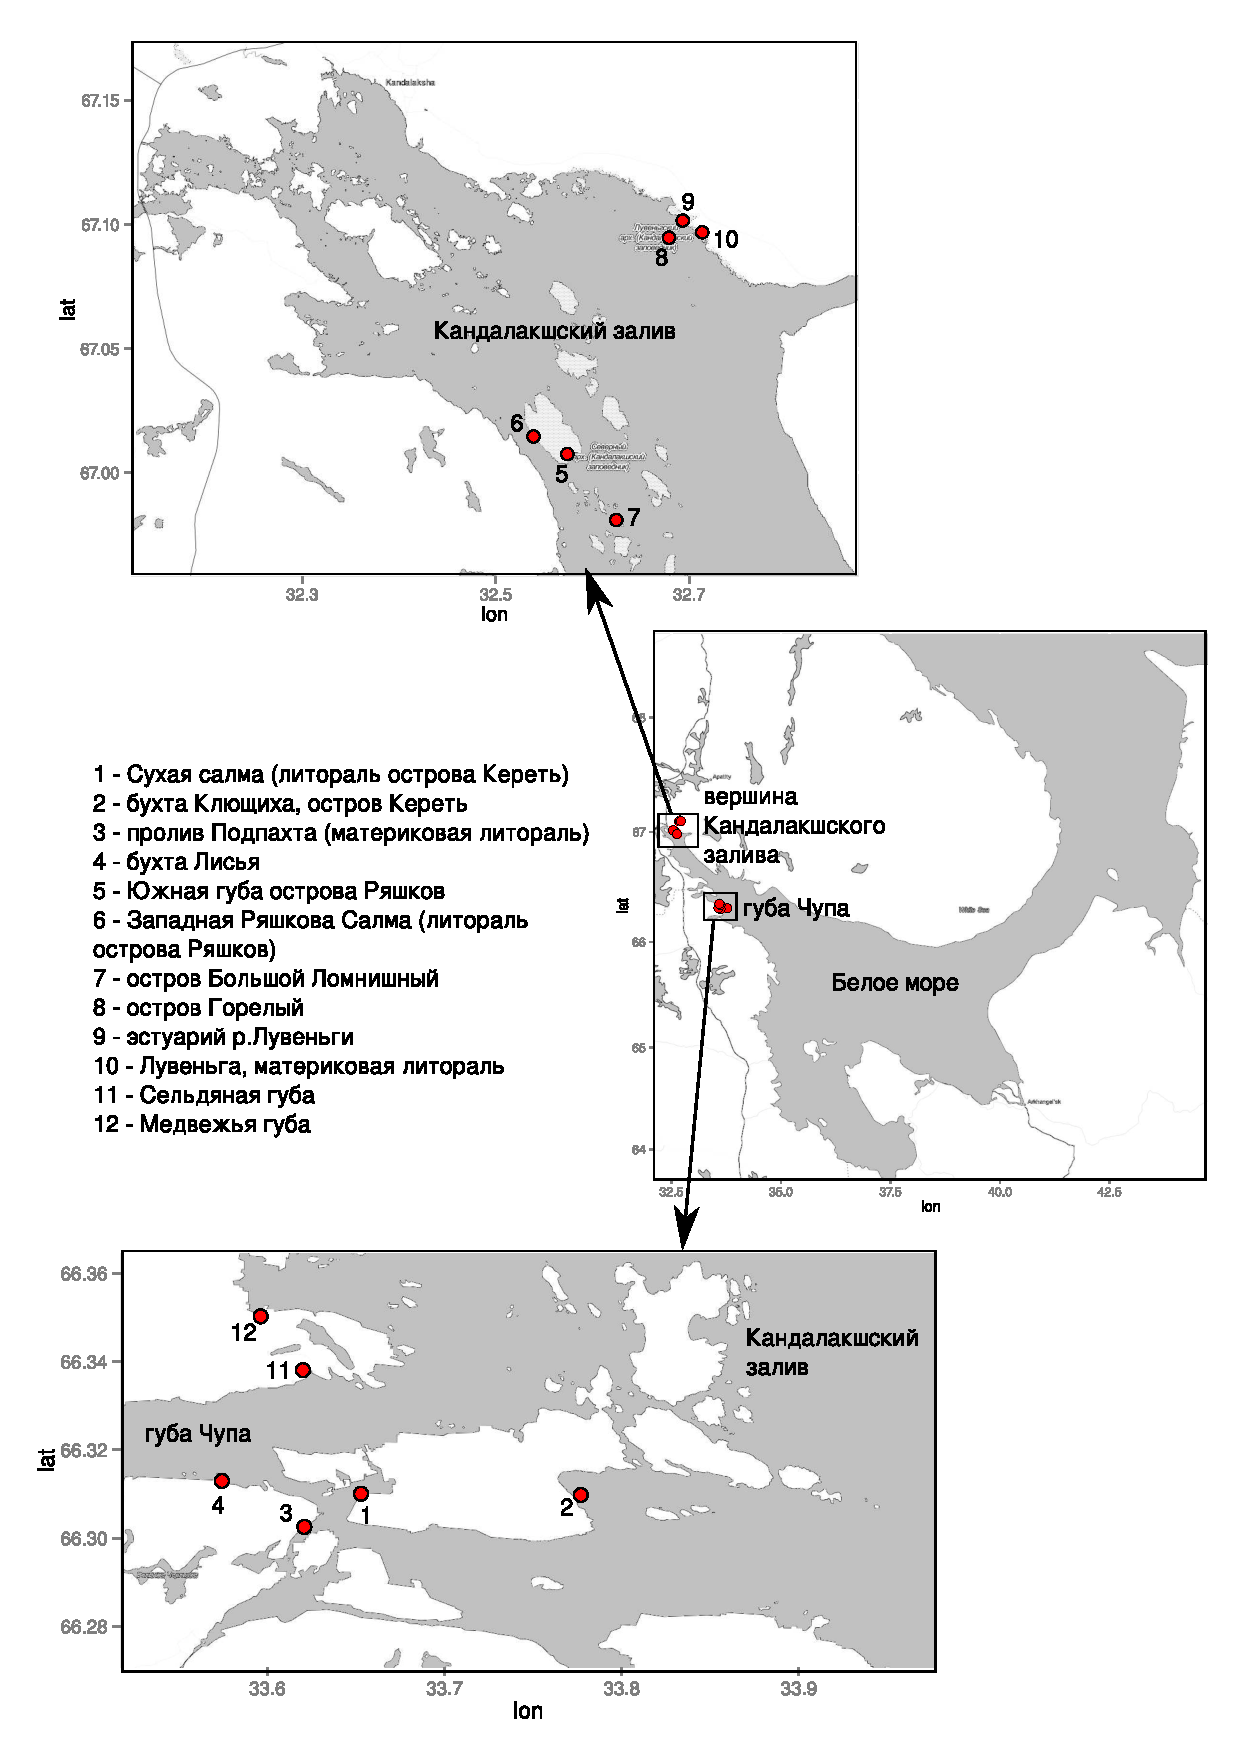
\includegraphics[width=\textwidth]{../maps/White_sea1.pdf}
    \caption{Исследованные участки в Кандалакшском заливе Белого моря}
    \label{ris:karta_White}
	\end{figure}
Три участка расположены в районе Лувеньгских шхер: эстуарий реки Лувеньги, Илистая губа острова Горелого и участок материковой литорали в $800$ метрах западнее поселка Лувеньга (участки 1, 2 и 3).
Один участок был расположен на литорали острова Ряшков в Западной Ряшковой Салме (Северный архипелаг) (участок 4).
В работе использованы данные Д.\:А.~Аристова из Южной губы о.~Ряшков и с о.~Большой Ломнишный (Северный архипелаг) (рис.~\ref{ris:karta_White}, участки 5 и 6). 

В районе губы Чупа исследования проводили на $4$ участках (рис.~\ref{ris:karta_White}) в ходе экспедиций кафедры ихтиологии и гидробиологии СПбГУ. 
Два участка были расположены на литорали острова Кереть~--- в Сухой Салме и бухте Клющиха (участки 7 и 8). 
Один участок был расположен на материковой литорали пролива Подпахта и один --- в бухте Лисьей (участки 9 и 10).

%Также в работе использованы данные ББС <<Картеш>> ЗИН РАН по обилию маком в губах Медвежья и Сельдяная (\cite{Varfolomeeva_Naumov_2013}) (рис.~\ref{ris:karta_White}, участки 11 и 12).

Все карты созданы с использованием данных OpenStreetMap (www.openstreetmap.org).
\afterpage{\clearpage}

		\subsection{Баренцево море}
Материал  в акватории Баренцева моря  был  собран    в ходе   студенческой баренцевоморской экспедиции СПбГУ. 
Всего было исследовано $8$ участков~--- $2$ в Кольском заливе и   $6$  в   прибрежной   зоне  Восточного  Мурмана (рис.~\ref{ris:karta_Barents}).  
	\begin{figure}[p]
    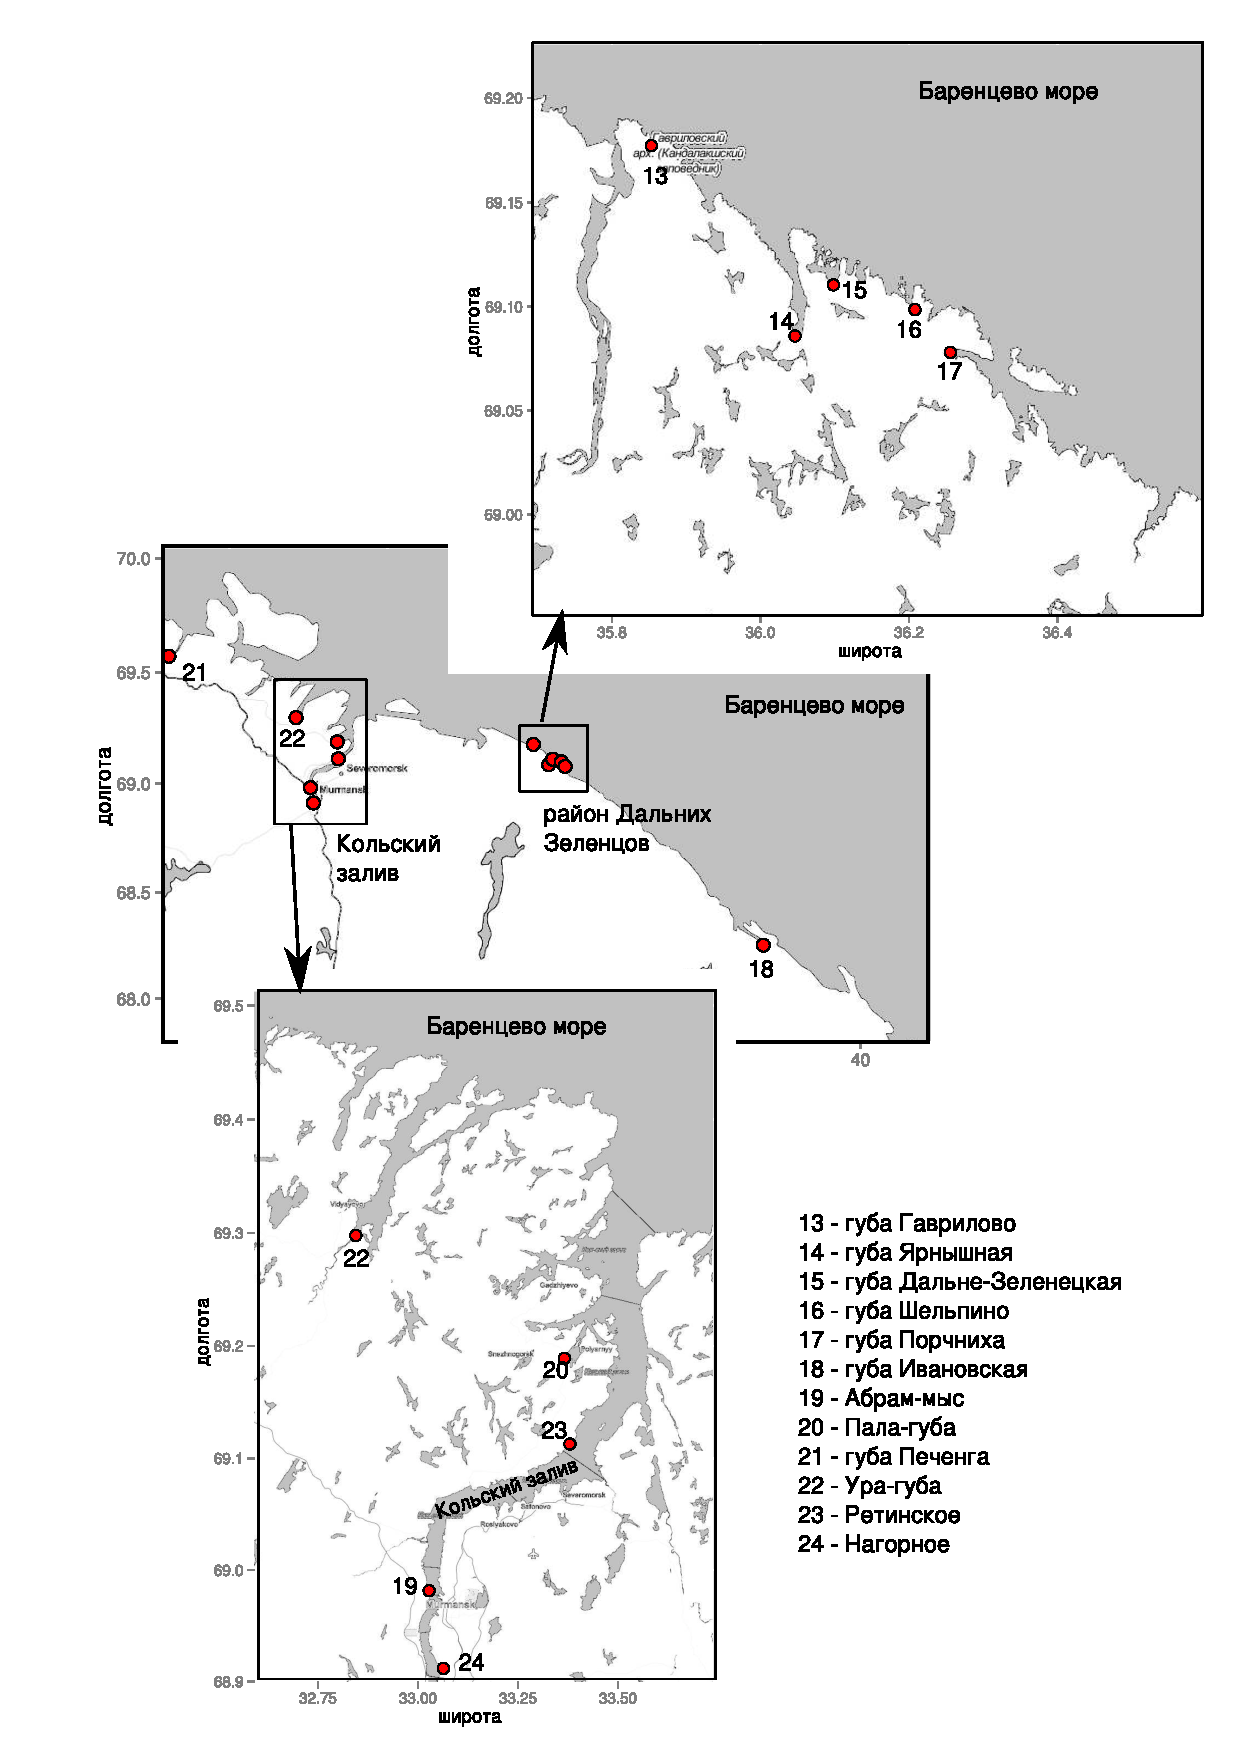
\includegraphics[width=\textwidth]{../maps/Barents_sea1.pdf}
    \caption{Исследованные участки вдоль Мурманского побережья Баренцева моря}
    \label{ris:karta_Barents}
	\end{figure}
На   Восточном   Мурмане исследованные участки литорали  были   расположены   в   губах   Гавриловская (участок 13),  Ярнышная (участок 14), Дальне-Зеленецкая (участок 15), Шельпинская (участок 16), Порчниха (участок 17) и Ивановская (участок 18).
Участки литорали  в   Кольском   заливе   были  расположены на побережье в районе Абрам-мыса (участок 19) и в Палa-губе (участок 20), в районе города Полярный. 


Также в работе использованы данные К.\:В.~Шунькиной и Е.\:А.~Генельт-Яновского по обилию маком в губе Печенга и Ура-губе (Западный Мурман) (рис.~\ref{ris:karta_Barents}, участки 21 и 22), и в районе Северного Нагорного и Ретинского (Кольский залив) (рис.~\ref{ris:karta_Barents}, участки 23 и 24).

\afterpage{\clearpage}

    \section{Характеристика местообитаний}
Для всех участков было составлено физиономическое описание.
На каждом участке измеряли ширину литорали.
По горизонтам описывали визуально тип грунта, наличие валунов, бурых водорослей, взморника \textit{Zostera marina}, зеленых нитчатых водорослей. 
Также описывали поясность сообществ, если она была выражена.
Термогалинные характеристики для отдельных участков не были описаны, и мы использовали литературные данные о среднегодовых параметрах для акваторий, и опубликованные данные о динамике температур в исследованный период (\cite{KGZ_letopis, rp5_Kandalaksha, pinro}.

Показательной комплексной оценкой гидродинамики региона и условий питания детритофагов служат показатели состава грунта. 
Поэтому на ряде исследованных участков были отобраны образцы грунта. 
В Белом море грунт исследовали на обоих участках в губе Чупа и на трех участках в вершине Кандалакшского залива.
В Баренцевом море грунт исследовали на всех участках Восточного Мурмана и двух участках Кольского залива (Абрам-мыс и Пала-губа).

Пробы грунта отбирали на всех исследованных горизонтах каждого участка.
В экспедиции после отбора из грунта выбирали крупных животных (червей, раков, моллюсков, приапулид), образцы высушивали и упаковывали для отправки в город. 
В городе образцы досушивали в термостате при температуре $105^o$C до момента, когда масса образца переставала изменяться. 
Из каждого образца брали по три навески грунта для определения содержания органических веществ. 
Навески помещали в муфельную печь с температурой $450^o$C на $8$ часов. 
После сжигания навески повторно взвешивали, и по разнице масс определяли массовую долю органических веществ в грунте. 
По трем навескам рассчитывали среднюю массовую долю для каждого образца.

Оставшийся грунт использовали для определения гранулометрического состава. 
При описании гранулометрического состава грунта использовали классификацию И.\,Л.~Безрукова и А.\,Н.,~Лисицина для морских водоемов (таблица~\ref{tab:lisicyn_granulometriya}, \cite{Bezrukov_Lisicyn_1960}).
\begin{table}[p]
    \centering
    \caption{Классификация фракций грунта по размеру частиц (\cite{Bezrukov_Lisicyn_1960})}
    \label{tab:lisicyn_granulometriya}
\begin{tabular}{|l|l|}
    \hline
    Размер фракции,~мм & Название фракции         \\ \hline
     $> 10$    & Крупный и средний гравий  \\
    $10-5$               & Мелкий гравий         \\
    $5-3$                & Очень мелкий гравий   \\
    $3-1$                & Очень крупный песок   \\
    $1-0,5$              & Крупный песок         \\
    $0,5-0,25$           & Средний песок         \\
    $0,25-0,1$           & Мелкий песок          \\
    $< 0,1$           & алевриты       \\\hline
\end{tabular}
\end{table}
Для этого грунт взвешивали, после чего просеивали в сухом состоянии через колонку сит (диаметр ячеи: $10 - 5 - 3 - 1 - 0,5 - 0,25$~мм). 
Частицы размером менее $0,25$~мм просеивали через сито с диаметром ячеи $0,1$~мм с использованием струи воды, после чего оставшиеся на сите --- высушивали при температуре $105^o$C. 
Каждую фракцию частиц взвешивали, и определяли их массовую долю. 
Анализ частиц размером менее $0,1$~мм (алевритов)не проводили. 

\afterpage{\clearpage}

    \section{Описание сообществ, включающих {\it Macoma balthica}}
На 6 мониторинговых участках в Кандалакшском заливе Белого моря проводили качественное описание фауны в пределах обследованных горизонтов литорали.
Таким образом, всего составлено $12$~описаний.
На каждом участке в акватории Баренцева моря исследовали все  горизонты литорали, представленные мягкими грунтами.  
Таким образом, всего было составлено $16$ описаний.

Как основное орудие сбора использовали литоральную рамку площадью $1/30$~м$^2$, из которой изымали грунт на глубину $5$~см. 
В случае, когда приходилось отбирать пробы из-под воды, использовали зубчатый водолазный дночерпатель площадью захвата $1/20$~м$^2$.
Отобранные пробы промывали на сите с диаметром ячеи $1$~мм. 

После промывки из   проб   выбирали   всех   особей  {\it M.~balthica}  и   представителей   сопутствующего макрозообентоса    для   определения   состава   сообщества.
Представителей   сопутствующего макрозообентоса  определяли   до   минимально   возможного   таксона. Таксономию и номенклатуру сверяли по Всемирному регистру морских видов (\cite{WoRMS}).

Для сравнения видового состава сообщества использовали коэффициент Жаккара. 
Результаты визуализировали при помощи  кластерного анализа методом ближайшего соседа. 
Достоверность выделенных групп оценивали с помощью анализа сходства профилей (SIMPROF) (\cite{Clarke_et_al_2008}).
Для оценки влияния факторов использовали многомерное шкалирование MDS в сочетании с анализом сходства ANOSIM.
Анализы проводили в программе PaSt (\cite{Hammer_et_al_2001}) и \R{} (\cite{R_2014}).

Кроме того, на литорали губы Дальне-Зеленецкой в $2002 - 2007$ проводили описание структуры сообщества. 
Для этого  в $2002$ году была заложена сеть из 8 станций (\cite{Genelt_Dalnezeleneckaya_2008}).
В пределах каждой станции отбирали 3 пирамиды рамок 1/245 + 1/30~м$^2$. 
Пробы площадью 1/245~м$^2$ промывали на сите с диаметром ячеи $0,5$~мм, внешние пробы площадью 1/30~м$^2$~--- на сите с диаметром ячеи 1~мм.  
Для проб площадью 1/245~м$^2$ проводили полную количественную разборку с последующей таксономический идентификацией особей и их подсчетом. 
В пробах  площадью 1/30~м$^2$ учитывали крупные виды Polychaeta и всех Bivalvia. 
Также в районе каждой станции отбирали по 3-5 проб площадью 1/10~м$^2$, которые также промывали на сите с диаметром ячеи 1~мм, для учета двустворчатых моллюсков.  У всех двустворчатых моллюсков измеряли длину раковины с точностью 0,1~мм.
Для выделения сообществ использовали анализ сходства профилей (SIMPROF) по матрицам коэффициентов Брея-Кертиса (данные по численности видов) (\cite{Clarke_et_al_2008}). 
Для множественного сравнения средних использовали непараметрический тест Краскела-Уоллиса.
Сравнение современных значений плотности поселений со значениями $1973$ года проводили, оценивая $2,5$ и $97,5$~\% квантили распределений плотности поселений в 2002-2007 годах.


%	\subsection{Изучение микрораспределения {\it Macoma balthica}}

%\textcolor{red}{квадраты на Белом}

%\textcolor{red}{квадраты на Баренцевом}
%При оценке распределения особей в губе Порчниха в 2007 г. было отобрано 32 пробы рамкой 1/30м2, причем пробы брались вплотную друг к другу 4 рядами по 8 шт.

% из Генельт-Кобылков-Назарова, 2007 (что это было??)
%Изучение распределения особей {\it Macoma balthica} было проведено в Баренцевом море по методике, описанной Трашем (\cite{Thrush_et_al_1989}) с изменением масштаба.
%Исследования были проведены в августе $2007$~г. на илисто-песчаной литорали кутовых участков губ Восточного Мурмана --- Ярнышной и Дальне-Зеленецкой, и в октябре $2007$~г. на литорали Пала-губы (Кольский залив). 
%Для Дальне-Зеленецкой губы съемка была повторена в августе $2008$ года на полигоне двойного размера.

%В каждой точке отбиралось по $36$ проб площадью $1/30$~м$^2$, расположенных в пределах участка размером $7,5 \times 12$~м. 
%Координаты каждой пробы были определены в декартовой системе координат в метрах, один из углов участка служил точкой отсчета. 
%В дальнейшем пробы промывали на сите с диаметром ячеи $1$~мм. 
%В лаборатории были выбраны и  подсчитаны все макомы.

%При дальнейшей обработке данных для каждого участках подсчитывали индекс структурности (отношение дисперсии к средней арифметической). 
%Для анализа размеров агрегаций были построены коррелограммы, основанные на коэффициенте пространственной автокорреляции Морана (\cite{ncf}).
%Достоверность коэффициентов определяли пермутационным методом.
%Наличие градиентов проверяли с использованием корреляционного анализа Кендалла между координатами проб и обилием вида в каждой пробе. 
%Все статистические анализы проводили в статистической среде \R{} (\cite{R_2014}) с $95\%$ доверительной вероятностью ($P < 0,05$).
%Для интерпретации результатов корреляционного анализа были использовали пузырьковые диаграммы.

\afterpage{\clearpage}	

	\section{Изучение структуры поселений {\it Macoma balthica}}
Для описания структуры поселений использовали данные всех доступных сборов.

В Белом море всего было обследовано $10$ участков в акватории Кандалакшского залива. 
На шести из них наблюдения проводили на всех горизонтах литорали, представленных мягкими грунтами.
На четырех других были обследованы отдельные горизонты. 

Для Баренцева моря были использованы данные по обилию с $12$ участков. 
На каждом участке в акватории Баренцева моря исследовали все  горизонты литорали, представленные мягкими грунтами.  

Как основное орудие сбора использовали литоральную рамку площадью $1/30$~м$^2$, из которой изымали грунт на глубину $5$~см. 
В случае, когда приходилось отбирать пробы из-под воды, использовали зубчатый водолазный дночерпатель площадью захвата $1/20$~м$^2$.
Отобранные пробы промывали на сите с диаметром ячеи $1$~мм или $0,5$ (на трех мониторинговых участках в районе Лувеньги и в Западной Ряшковой Салме, участки $7, 8 - 10$ на рис.~\ref{ris:karta_White}). 
После промывки из   проб   выбирали   всех   особей  {\it M.~balthica}.
Подробная информация о количестве проб и размере учетных площадок для каждого участка представлены в приложении~\ref{app:NB_table}.

В дальнейшем подсчитывали количество особей в пробах, которое пересчитывали в плотность поселения моллюсков на квадратный метр. 
Для всех средних значений рассчитывали точность учета $d,\% = m/M$, где $m$~--- стандартная ошибка средней, $M$~--- средняя арифметическая.
Биомассу определяли путем взвешивания на весах с точностью 10 мг, либо, для части участков на Белом море, расчетным методом.
Мы использовали формулу зависимости массы макомы от ее длины $W = 0,00016 \times L^{2,96}$, полученную для губы Чупа (\cite{Maximovich_et_al_1993}).


Изучение размерной структуры поселений маком проводили на всех участках.
Для этого у всех моллюсков в пробах под бинокуляром измеряли максимальный линейный размер (длину) с точностью $0,1$~мм.
По полученным данным строили размерно-частотное распределение с шагом $1$~мм.

%Кроме того, на части участков у моллюсков подсчитывали количество меток зимней остановки роста, которое принимали как возраст моллюсков --- число прожитых зим (например, $4+$ это  особи возрастом от $4$ до $5$ лет).   
%Таким   образом   были   получены   оценки возрастной структуры поселений {\it M. balthica}.

Для визуализации данных по обилию использовали графики Тьюки (Tukey boxplots, \cite{Tukey_1977}). 
Сравнение обилия проводили с помощью непараметрического теста Краскела-Уоллиса. 
Для выявления связи величин обилия с гранулометрическим составом грунта использовали непараметрическую корреляцию Спирмена (\cite{Hollander_et_al_2013}).
Классификацию размерных структур проводили с помощью анализа главных компонент (\cite{Mardia_et_al_1979}).
Все анализы проводили в статистической среде \R{} (\cite{R_2014}).

\afterpage{\clearpage}

	\section{Изучение динамики поселений {\it Macoma balthica}}
        \subsection{Белое море}
В Белом море динамику поселений {\it Macoma balthica} исследовали на $6$ участках в районе вершины Кандалакшского залива. 

Сборы проводили с 1992 по 2012 год ежегодно в июле-августе.
Автор принимала участие в полевых сборах с $1999$ по $2007$ год.
Данные за другие годы взяты из архива ГИПС ЛЭМБ.

Структура материала представлена в таблице \ref{tab:material_Kandalaksha}.
\begin{table}[p]
\caption{Структура материала по динамике поселений {\it Macoma balthica} вершины Кандалакшского залива}
\label{tab:material_Kandalaksha}
%\begin{tabular}{|*{5}{p{0.2\textwidth}|}} \hline
    \begin{tabularx}{\textwidth}{|*{5}{X|}} \hline
участок & годы наблюдения & обследованные горизонты литорали & количество проб в однократной съемке & площадь пробоотборника, м$^2$  \\ \hline
о. Горелый Лувеньгских шхер & 1992 -- 2012 & ВГЛ, СГЛ, НГЛ & 1-3 & 1/30, 1/10 \\ \hline
Материковая литораль в районе пос. Лувеньга & 1992-2000, 2002, 2004 & ВГЛ, СГЛ, НГЛ & 12-20 & 1/30 \\ \hline
Эстуарий р. Лувеньги & 1992 -- 2012 & СГЛ & 3 & 1/10 \\ \hline
Литораль Западной Ряшковой Салмы о. Ряшкова & 1994 -- 2012 & СГЛ & 2 & 1/10 \\ \hline
Южная губа о. Ряшкова & 2001 -- 2012 & НГЛ & 9-16 & 1/30 \\ \hline
о. Ломнишный & 2007 -- 2012 & НГЛ & 5-10 & 1/30  \\ \hline
\end{tabularx}
\end{table}

На каждом исследованном участке отбирали $3 - 25$ проб площадью $1/30 - 1/10$~м$^2$, которые затем промывали на сите с диаметром ячеи $0,5 - 1$~мм. 
В пробах учитывали всех особей {\it M.~balthica}, у которых в дальнейшем измеряли максимальный линейный размер (длину) с точностью ~0,1~мм. 

Для определения биомассы моллюсков взвешивали на электронных весах с точностью до $1$~мг. 
Для серий проб, где не проводили взвешивание моллюсков, биомассу определяли расчетным методом с использованием аллометрической зависимости сырой массы маком от длины их раковины (\cite{Maximovich_et_al_1993}). 

В дальнейшем рассчитывали среднюю плотность поселений и строили размерно-частотное распределение особей.
Для построения размерно-частотного распределения шаг размерного класса составлял $1$~мм.

В дальнейшем при анализе мы работали с особями с длиной раковины более $1,0$~мм по двум причинам. 
Во-первых, для того чтобы сделать сравнимыми результаты с разных участков, где пробы промывались на ситах с разным диаметром ячеи. 
Во-вторых, пробы отбирали в середине лета, то есть к этому моменту молодь этого года частично осела, то есть оценка численности данной группы будет некорректна.
Мы считаем корректной такую редукцию материала, поскольку для Белого моря считается, что успешность пополнения поселений молодью в первую очередь зависит от выживаемости спата зимой (\cite{Maximovich_Gerasimova_2004}).

Для анализа динамики пополнения поселений молодью в $2012 - 2013$ годах у особей длиной менее $3$~мм были измерены длины колец зимней остановки роста. 
После определения размеров годовалых особей, по размерной было рассчитано их обилие в каждом году мониторингового наблюдения.
Всего было промерено 496 особей.



В работе использованы мониторинговые данные кафедры ихтиологии и гидробиологии СПбГУ по обоим участкам на острове Кереть (\cite{Maximovich_et_al_1991, Gerasimova_Maximovich_2013}) (рис.~\ref{ris:karta_White}, участки $1, 2$). 
Также в работе использованы многолетие данные ББС <<Картеш>> ЗИН РАН по обилию маком в губах Медвежья и Сельдяная (\cite{Varfolomeeva_Naumov_2013}) (рис.~\ref{ris:karta_White}, участки $11, 12$).


 
%методика из Назаровой-Полоскина
%Материал собран в августе 1992 - 2003 гг. Изучено три литоральных поселения маком: в Илистой губе острова Горелого (участок 1), в эстуарии реки Лувеньги (участок 2) и на материковой литорали к югу от поселка Лувеньга (участок 3). Сборы проведены пробоотборником площадью захвата 1/30 м2. Разовая выборка составляла от 9 до 25 проб с участка. Грунт выбирался до глубины 5 см и промывался на сите с диаметром ячеи 0.5мм.  Всех особей  M. balthica измеряли с точностью 0.1 мм. В каждый момент наблюдений определяли размерную структуру и плотность поселения маком. 



% методика из Аристова
%Оба участка закрыты от волнового воздейст-
%вия. Литораль в районе исследований представляет собой песчаный пляж с примесью
%ила с вкраплениями крупных валунов. Спуск в сублитораль пологий, отчетливо вы-
%раженный пояс фукоидов отсутствует. Население представлено типичными формами,
%такими как Arenicola marina, Macoma balthica, Mya arenaria, Hydrobia ulvae, Microspio sp.
%и др. (Д. А. Аристов, неопубликованные данные).
%В обеих точках производили сборы по следующей методике: в районе нуля глубин
%во время отлива в пределах участков случайным образом выбирали и обследовали не-
%сколько площадок. Поскольку радиусы индивидуальной активности A. islandica и пред-
%полагаемых жертв (двустворчатых моллюсков) существенно различаются, в пределах
%каждой площадки брали пару проб методом вложенных рамок. Первую пробу из пары
%(1/4 м2) брали для учета A. islandica. Грунт из пробы тщательно перебирали вручную,
%всех найденных представителей сем. Naticidae подсчитывали и определяли их видовую
%принадлежность. Вторая проба (1/30 м2) была взята для учета потенциальных жертв —
%двустворчатых моллюсков. Грунт из нее промывали на сите с диаметром ячеи 1 мм,
%а затем остаток разбирали в фотографической кювете с белым дном. Из грунта соби

\afterpage{\clearpage}

        \subsection{Баренцево море}
% из Дерюгинских, 2007 + новой статьи

В Баренцевом море динамику поселений маком исследовали на модельном участке --- литоральной отмели Дальний пляж губы Дальне-Зеленецкой. 
В работе использованы материалы экспедиции по мониторингу Дальнего пляжа губы Дальне-Зеленецкой с $2002$ года, любезно предоставленные Е.\:А.~Генельт-Яновским.
Автор принимала участие в полевых сборах в $2006 - 2008$~гг.

Материал был собран в июле-августе $2002 - 2008$~гг. в пределах от верхнего горизонта песчаной литорали ($+2,0$~м) до $+0,7$~м над нулем глубин. 

 В $2002$ году была заложена сетка из $8$ станций. 
 В пределах каждой станции отбирали $3 - 5$ проб площадью $1/10$~м$^2$, которые промывали на сите с диаметром ячеи $1$~мм. 
 У всех двустворчатых моллюсков измеряли длину раковины с точностью $0,1$~мм. 
 С 2004 года отбирали пробы на трех станциях из $8$, которые располагались в контрастных сообществах (\cite{Genelt_Dalnezeleneckaya_2008}). 

В качестве точки сравнения нами был выбран $1973$ год (\cite{Streltsov_et_al_1974, Agarova_et_al_1976}), поскольку в тот год была проведена основная количественная съемка на Дальнем пляже. 

 %Восстановление возрастной структуры {\it Macoma balthica} для 2002-06 годов было проведено по моллюскам из выборки 2007 года. Для этого у них были измерены кольца зимней остановки роста и рассчитаны размеры моллюсков каждой возрастной группы. В качестве границ размерно-возрастных классов принималась середина соответствующего размерного диапазона. В дальнейшем, в зависимости от длины, каждого моллюска из выборок 2002-06 гг. относили к определенному возрастному классу. Так как в 2007 году не были встречены особи с 8 видимыми кольцами зимней остановки роста, то все особи крупнее 17,7 мм (верхняя размерная граница возрастного класса 8+) были объединены в одну группу.

Сравнение средних проводили с помощью критериев Вилкоксона и Краскела-Уоллиса (\cite{Hollander_et_al_2013}).
При анализе трендов в динамике поселений использовали корреляционный анализ Мантеля (\cite{Legendre_Legendre_2012}) для удаления тренда из рядов. 
Также данный метод использовали для оценки синхронности динамик обилия моллюсков в разных поселениях.
Для выявления плотностнозависимых процессов были использованы частные автокорреляции (PRCF --- Partial rate correlation function) (\cite{Berryman_Turchin_2001}).
Для изучения влияния температуры на динамику обилия \textit{M.~balthica} использовали линейные модели (\cite{Chambers_Hastie_1991}).
Оценку корректности построенной модели проверяли с помощью критериев Дарбина-Уотсона (отсутствие автокорреляций), Шапиро-Уилка (нормальное распределение остатков) и Бройше-Пагана (гомогенность дисперсий).
Все расчеты проводили в статистической среде \R{} (\cite{R_2014}).

\afterpage{\clearpage}

	\section{Изучение линейного роста {\it Macoma balthica}}
%из статьи про рост
Рост \textit{M.~balthica} в Белом море достаточно детально изучен (\cite{Semenova_1970, Maximovich_et_al_1992, Hummel_et_al_1998}), поэтому мы проводили специальные исследования только для Баренцева моря.

Рост изучали по материалам, полученным в августе $2007 - 2008$~гг. для $7$ участков в Баренцевом море: Абрам-мыс, Пала-губа, губы Гавриловская, Ярнышная, Дальне-Зеленецкая, Шельпино, Порчниха.
Станции для отбора проб располагали по горизонтам литорали. 

У всех особей {\it Macoma balthica} в пробах ($1/30$ или $1/20$~м$^2$, промывка на сите с диаметром ячеи 1~мм) измеряли длину (наибольший линейный размер) раковины и (по меткам роста) ее значения в период каждой зимней остановки роста с точностью 0,1 мм.
Полученные для каждой станции измерения особей были сведены в описание возрастной структуры по схеме, представленной в табл.~\ref{tab:rost_matrica_primer}. 
\begin{table}[p]
        \caption{Пример треугольной матрицы с данными по росту моллюсков и их возрастной структуре}
        \label{tab:rost_matrica_primer}
%    \begin{tabular}{|c|c|cc|cc|ccccccccc|}
        \begin{tabularx}{\textwidth}{|X|X|XX|XX|XXXXXXXXX|}
        \hline
        &    & \multicolumn{4}{c|}{$L$}               & \multicolumn{9}{c|}{$L_{k}$} \\ 
        $t$     & $N$  & $min$ & $max$ & $aver$ & $m_{L}$   & 1 к & 2к  & 3к  & 4к  & 5к  & 6к  & 7к  & 8к   & 9к   \\ \hline
        0+      & 0  &       &       &         &         &     &     &     &     &     &     &     &      &      \\
        1+      & 9  & 1,8   & 2,5   & 2,2     & 0,1     & 1,1 &     &     &     &     &     &     &      &      \\
        2+      & 76 & 1,6   & 7,9   & 3,1     & 0,1     &\cellcolor{yellow}0,7 & \cellcolor{yellow}2,0 &     &     &     &     &     &      &      \\
        3+      & 40 & 2,1   & 5,8   & 3,8     & 0,1     & 0,7 & 1,8 & 2,9 &     &     &     &     &      &      \\
        4+      & 34 & 2,1   & 8,5   & 5,4     & 0,2     & 0,7 & 1,8 & 3,1 & 4,6 &     &     &     &      &      \\
        5+      & 37 & 3,5   & 9,8   & 6,8     & 0,2     & 0,8 & 1,9 & 3,1 & 4,6 & 6,2 &     &     &      &      \\
        6+      & 44 & 4,6   & 11,5  & 8,2     & 0,2     & 0,8 & 1,8 & 2,9 & 4,1 & 5,5 & 7,3 &     &      &      \\
        7+      & 48 & 7,4   & 12    & 9,9     & 0,2     & 0,9 & 2,1 & 3,3 & 4,6 & 6,0 & 7,7 & 9,1 &      &      \\
        8+      & 61 & 8     & 13,7  & 10,6    & 0,1     & \cellcolor{red}0,7 & \cellcolor{red}2,0 & \cellcolor{red}3,4 & \cellcolor{red}4,6 & \cellcolor{red}6,1 & \cellcolor{red}7,5 & \cellcolor{red}8,9 & \cellcolor{red}9,9  &      \\
        9+      & 44 & 8,6   & 14,2  & 11,1    & 0,2     & -   & -   & 3,4 & 4,7 & 6,5 & 8,2 & 9,7 & 10,5 & 11,4 \\ \hline
                &    &       &       & $L_{k} aver$  &  & \cellcolor{blue}0,8 & \cellcolor{blue}1,9 & \cellcolor{blue}3,1 & \cellcolor{blue}4,5 & \cellcolor{blue}6,0 & \cellcolor{blue}7,7 & \cellcolor{blue}9,2 & \cellcolor{blue}10,2 & \cellcolor{blue}11,4 \\
                &    &       &       & $m_{Lк}$      &  & 0,0 & 0,0 & 0,1 & 0,1 & 0,2 & 0,2 & 0,3 & 0,4  &      \\
                &    &       &       & $L_{k} min$  &   & 0,7 & 1,8 & 2,9 & 4,1 & 5,5 & 7,3 & 8,9 & 9,9  &      \\
                &    &       &       &  $L_{k} max$ &   & 1,1 & 2,1 & 3,4 & 4,7 & 6,5 & 8,2 & 9,7 & 10,5 &     \\ \hline
    \end{tabularx}
    \footnotesize{Примечания: $t$ --- возраст моллюсков; 
        $N$ --- количество  особей  данного возраста, экз.; 
        $L min$  ---  минимальная   длина  особей   данного   возраста,   мм;   
        $L max$   ---   максимальная   длина   особей   данного   возраста,   мм; 
        $L aver$ --- средняя длина моллюсков данного возраста, мм; 
        $m_L$ --- ошибка средней, 
        $L_k$ 1к -- 13к --- длина особи к определенному возрасту, измеренная по меткам зимней остановки роста, мм;
        $L_k aver$ --- средняя длина данной метки остановки роста, мм; 
        $m_{L_k}$ --- ошибка средней; 
        $L_k min$ --- минимальная длина данной метки остановки роста, мм; 
        $L_k   max$   --   максимальная   длина   данной   метки   остановки   роста.   
        В   таблице   приведены средние длины данного кольца у моллюсков определенного возраста. \\[1em]
    Выделения: синий --- средневзвешенный возрастной ряд для маком в данном поселении;
        красный --- возрастной ряд отдельной генерации маком;
        желтый --- средний годовой прирост моллюсков в определнном возрасте}
\end{table}
Таким образом, всего было получено $14$ описаний, условно характеризующих отдельные поселения маком. 
Как видно из данных табл.~\ref{tab:rost_matrica_primer}, каждое из описаний содержало результаты реконструкции динамики средней длины раковины маком в генерациях. 
Эти данные мы использовали для сравнительного анализа характера линейного роста моллюсков в поселениях и расчета величин группового годового прироста особей в генерации (как разность средних длин раковин моллюсков в последовательные моменты зимней остановки роста).

Возрастные ряды аппроксимировали при помощи линейной модификации уравнения Берталанфи: $L_{t} = L_{max} \times (1 - e^{(-k(t - t_{0}))})$, где $L_{max}$, $k$, $t_{0}$ --- коэффициенты, $t$ --- возраст, а $L_{t}$ --- длина раковины моллюска в возрасте $t$.
Сравнительный анализ кривых роста произведен с учетом разброса эмпирических данных относительно регрессионной модели. 
В качестве меры расстояния использовали отношение величины статистики $F$ (частное от деления остаточной вариансы относительно кривой роста на сумму остаточных варианс относительно частных моделей роста) к $5$\%-ному квантилю $F$-распределения (\cite{Maximovich_1989}). 
Расчеты проводили при помощи оригинального макроса к MS Excel, выполненного Т.С.~Ивановой.
При сравнении авторских данных с литературными источниками использовали как вышеописанную методику, так и сравнение параметра $\omega = L_{\infty} \times k$ (где $L_{\infty}$ и $k$ --- коэффициенты уравнения роста Берталанфи), который считается более адекватным для задач сравнения ростовых характеристик, чем сравнение параметров уравнения Берталанфи напрямую (\cite{Appeldoorn_1983, Beukema_Meehan_1985}). 

Структуру вариансы величин группового годового прироста анализировали при помощи двухфакторного дисперсионного анализа (\cite{Chambers_Hastie_1991}). 
Как факторы влияния рассматривали начальную для данного интервала среднюю длину раковины, местообитания (участок) и мареографический уровень положения станции (горизонт литорали).
В статистических расчетах ориентировались на уровень значимости критерия $\alpha < 0,05$.
Расчеты проводили в Statistica for Windows.

\afterpage{\clearpage}

	\section{Изучение спата и пополнения поселений {\it Macoma balthica}}
Для исследования количественного формирования спата было выбрано $4$ участка, различных по абиотическим условиям (рис.~\ref{ris:karta_White}, участки 1-4). 
Выбор был обусловлен тем, что все эти участки уже изучали до этого, на двух из них ведется мониторинг силами сотрудников кафедры ихтиологии и гидробиологии. 
Все участки характеризуются мягкими грунтами, и по данным предшествующих наблюдений, на них существуют стабильные во времени плотные поселения маком.
Съемки проведены в июле и в конце августа $2006$ года.

В июле на среднем горизонте литорали было отобрано по 5 проб на каждом участке для учета маком старше $1$ года. 
Размер учетных площадок составлял от $0,1$ до $0,05$~м$^2$. 
Пробы промывали на сите с диаметром ячеи $1$ мм. 
В пробах проводился количественный учет макробентоса, и определялась его биомасса.
У всех особей \textit{M.~balthica} под бинокуляром измеряли максимальный линейный размер (длину) раковины с точностью $0,1$~мм. 
Биомассу маком в дальнейшем рассчитывали с использованием формулы аллометрической зависимости индивидуальной сырой массы маком от длины раковины (\cite{Maximovich_et_al_1993}).

В конце августа на этих же участках были отобраны пробы с учетной площади $0,01$ кв. м, которые фиксировали, а затем без промывки разбирали под бинокуляром.  
Из данных проб выбирали всех особей \textit{M.~balthica}, осевших в этом году, т.е не имевших кольца остановки роста. 
В дальнейшем у всех плантиград измеряли длину. 

Статистическую обработку материала проводили по стандартным формулам в программах MS Excel 2003 и Statistica 6.0. 
Для выявления связи численности спата с обилием маком и с обилием макрозообентоса использовался ранговый коэффициент корреляции Спирмена ({\cite{Hollander_et_al_2013}).

Для оценки влияния плотности поселения взрослых маком на размеры пополнения был проведен иерархический дисперсионный анализ  (\cite{Chambers_Hastie_1991}).
Фактор <<плотность поселения взрослых особей>> (N взр.) был представлен в двух градациях: <<высокая>> (более $1000$~экз./м$^2$) и <<низкая>> (менее $600$~экз./м$^2$).
В качестве вложенного фактора использовался <<участок>>: Сухая Салма и бухта Лисья как участки с высокой плотностью и бухта Клющиха и пролив Подпахта~--- с низкой. 

Аналогичный дисперсионный анализ был проведен для отдельных размерных классов взрослых маком для выявления характера влияния на разноразмерных особей факторов <<плотность поселения взрослых особей>> и <<участок>>. 
В анализе использовали данные по количеству взрослых маком размером от $2$ до $9$~мм с шагом $1$~мм, т.к. именно особи этих размеров представлены в выборках в достаточном для анализа количестве.
Каждый дисперсионный анализ сопровождался оценкой силы влияния факторов с ошибкой и достоверностью. 

\par\medskip
Для изучения динамики пополнения поселения численность годовалых особей в каждый год была восстановлена по данным размерной структуры.
Для этого по данным мониторингов $2012 - 2013$ годов были проведены измерения длин колец зимней остановки роста у особей длиной менее $3$~мм.
Для сравнения полученных данных использовали критерий Краскела-Уоллиса, и в случае достоверных отличий --- тест Тьюки (Tukey’s ‘Honest Significant Difference’) ({\cite{Hollander_et_al_2013}).
Для определения границ размерно-возрастных классов {\it Macoma balthica} возрастом $0+$, $1+$ и $2+$ были рассчитаны средние размеры особей каждого возраста.
Пограничный размер между двумя когортами рассчитывали как середину между средними размерами особей в когорте.

На основании полученных данных о размере годовалых маком была рассчитана их плотность поселения в каждом году наблюдения.
Для выявления связи между обилием годовалых особей с различными параметрами использовали коэффициент корреляции Спирмена {\cite{Hollander_et_al_2013}).
Гипотезу о синхронности пополнения поселений в акватории проверяли при помощи корреляции Мантеля (\cite{Legendre_Legendre_2012}).
Все расчеты проводили в статистической среде \R{} (\cite{R_2014}).

\afterpage{\clearpage}

%%описание участков

    \section{Характеристика района исследования}
        \subsection{Географическое и физиономическое описание}
			\subsubsection{Белое море}

\paragraph{Участок материковой литорали, расположенный в 800 м к югу от поселка Лувеньга.}

Данный разрез имеет вид прямоугольника, длина которого ограничена $10$~метрами, а ширина равна ширине литорали в максимальный сизигийный отлив (72 метра). 
На данном участке пробы брались равномерно на протяжении всей ширины литорали. Описание разреза дано по работе А.~Полоскина (\cite*{Poloskin_1996}).

Верхняя часть литорали на разрезе представляет гравийно-мелкокаменистую осыпь со значительным наклоном дна, нижняя граница которой расположена в 
$10$~метрах от штормовых выбросов.

Ниже на литорали располагается пологий пляж с илистым песком с заметными вкраплениями крупного песка. 
Во время отлива здесь могут оставаться небольшие лужицы. 
В данном биотопе отмечены отдельные выбросы пескожилов {\it Arenicola marina} и кое-где тонкий мат зеленых нитчаток. 
В дальнейшем эта зона будет называться <<верхний пляж>>. 
На расстоянии $19$~метров от штормовых выбросов верхний пляж ограничивает валунная гряда.

За валунной грядой следует валунная россыпь с плотными поселениями фукоидов. 
Постепенно россыпь разреживается и между валунами появляются окна илисто-песчаного грунта. 
Плотность пояса фукоидов также постепенно уменьшается, и к $37$~метру от штормовых выбросов фукоиды и валуны практически полностью исчезают. 
В дальнейшем этот биотоп будет называться <<пояс фукоидов>>.

Ниже располагается следующий хорошо различимый биотоп --- пояс взморника {\it Zostera marina} (данное название сохранится за ним и далее). 
Плотное, почти со стопроцентным проективным покрытием, поселение этих растений на илисто-песчаном грунте простирается до $59$~метра от штормовых выбросов. 
Помимо взморника, в данном биотопе отмечено большое количество нитчатых водорослей с прикрепленных на них молодью мидий {\it Mytilus edulis}.

От $59$ до $72$~метра расположен участок, осушающийся только в сизигийный отлив на два с небольшим часа. 
Илисто-песчаный пляж данного биотопа служит местом обитания для поселений пескожила и большого количества мидиевых щеток. 
Данный биотоп будет именоваться <<нижний пляж>>. 


\paragraph{Участок в Илистой губе острова Горелого.}
Ширина литорали на данном участке составляет $24$~метра. 
Так как верхняя литораль характеризуется каменистым грунтом, то пробы брались только в среднем и нижнем горизонте литорали.
Верхняя часть литорали представляет собой гравийную россыпь, выходящую на приморский луг. 
Ниже (в среднем горизонте) следует илисто-песчаный пляж с редкими некрупными камнями и отдельными выбросами пескожилов.  
На расстоянии $15$~метров от линии штормовых выбросов появляются редкие вкрапления фукоидов (на границе среднего и нижнего горизонтов литорали) и увеличивается количество мелких камней, но  все же этот участок можно характеризовать как илисто-песчаный пляж. 
Плотность поселения {\it Arenicola marina} заметно увеличивается по сравнению со средним горизонтом.
На уровне $17-21$ метров от штормовых выбросов располагается валунная гряда с плотными поселениями фукоидов (нижний горизонт литорали). 
В данной зоне пробы отбирались на участках, не закрытых талломами водорослей. 
В районе нуля глубин на данном участке также характерен илисто-песчаный грунт с плотным поселением {\it Arenicola marina}.


\paragraph{Участок в эстуарии реки Лувеньги.}
На данном участке ширина литорали составляет $500$~метров. 
На всем протяжении это практически горизонтальный илисто-песчаный пляж с плотным поселением пескожилов. 
Так как этот участок расположен в эстуарии реки, то он характеризуется пониженной соленостью. 
В данном районе пробы брались на расстоянии $350$~метров от линии штормовых выбросов на нижнем горизонте литорали.


            \subsubsection{Баренцево море}

            \paragraph{Северное Нагорное}
Данный участок расположен в третьем колене Кольского залива, на южном его берегу в пределах одноименного района г.~Мурманск. 
Собственно литораль начинается за жилым массивом, в месте расположения опор моста через Кольский залив. 
Место сбора находилось в 600 м севернее моста. 
Ширина литорали на данном участке составляет $100$~м. 
Верхний горизонт литорали представлен небольшими валунами и россыпью гравия. 
Средний и нижний горизонты литорали представляют собой достаточно пологий илисто-песчаный склон с редкими валунами. 
Грунт достаточно сильно эвтрофицирован, очень вязкий. 
Между валунами встречаются поселения пескожила {\it Arenicola marina}.

            \paragraph{Абрам-мыс}
Участок  в районе  Абрам-мыса  находится в третьем колене Кольского залива, максимально удаленном от моря.
Абрам-мыс --- район   города   Мурманск,  расположенный   на противоположной стороне от основного городского массива, напротив порта. 
Исследованный участок   литорали   находился   в   $1,5$~км   к   выходу   из   залива   от   причала,   куда   приходит пассажирский катер. 
Ширина   литорали   на   данном   участке   составляет   $45$~м.   
Верхний   горизонт   литорали представлен  каменисто-галичной  россыпью. 
В среднем  горизонте литорали на поверхности илисто-песчаного   грунта   располагаются   валуны,   покрытые   фукоидами   ({\it Fucus  vesiculosus}), которые   формируют   практически   сплошной   покров   с   отдельными   «окнами»   грунта (проективное  покрытие фукоидов $90~\%$).  
При приближении  к нижнему горизонту литорали количество   валунов   уменьшается,   и   проективное   покрытие   фукоидов   составляет   здесь   не более $10~\%$.

    \paragraph{Ретинское}
Ретинское находится на западном берегу Кольского залива, напротив г.~Североморск. 
В береговую линию вдается небольшая, овальной формы губа. 
Ширина литорали составляет около $60$~м. 
Дно каменистое, между камнями --- илисто-песчаный грунт, достаточно промытый. 
На верхнем горизонте литорали располагаются крупные валуны, покрытые фукусами и балянусами, чуть ниже находятся крупные камни полностью покрытые фукоидами.
Средний и нижний горизонты литорали представлены среднего размера камнями, примерно половина из которых покрыта фукоидами. 

    \paragraph{Пала-губа}
Пала-губа   представляет   собой   глубоко   вдающуюся   в   берег   губу   длинным   узким «горлом», за которым следует расширение, формирующее несколько губ второго порядка. 
В «горле» расположен остров Шалим, и, таким образом, губа соединяется с Кольским заливом узкими   проливами.   
В   основной   части   Пала-губы   расположено   несколько   более   мелких островков. 
Исследованный участок располагался в длинной узкой губе (бухта Дровяная), закрытой на выходе островом Зеленый.
В кут губы впадает крупный ручей, формирующийся на литорали во время отлива оформленное русло, положение которого за два года наблюдений не изменилось.
Ширина литорали на данном участке составляет  $130$~м. 
Верхний горизонт литорали представлен   каменисто-валунной   россыпью,   которая   на   границе   со   средним   горизонтом становится более разреженной, и покрыта зарослями фукоидов ({\it Fucus vesiculosus}). 
Средний и нижний   горизонты   представлены   двумя   илисто-песчаными   пляжами,   разделенными каменисто-валунной грядой на месте резкого локального увеличения угла уклона свала. 
На нижней литорали грунт более заилен, и на поверхности располагаются агрегации {\it Mylius edulis} («мидиевые щетки»).

    \paragraph{Печенга}
Печенга расположена на Западном Мурмане, в $150$~км от границы с Норвегией. 
Собственно поселок находится на берегу сильно вдающейся в полуостров губы Печенга. 
Сбора материала производился в средней части этой губы, на удалении $1,5$~км от кута губы. 
Литораль на этом участке достигает ширины $50$~м. 
Верхний горизонт литорали представлен среднего размера валунами. 
На среднем горизонте валуны расположены более редко, а между ними находится россыпь достаточно крупного гравия. 
Нижний горизонт литорали илисто-песчаный. 

    \paragraph{Губа Гаврилово}
Гаврилово – наиболее западная губа из исследованных нами участков на Восточном Мурмане. 
Эта   губа   с  достаточно   широким   входом,   свободно   открывающаяся  в  Баренцево море.   
Восточную   ее   часть   несколько   закрывает   от   прибоя   мыс,   формирующий   «горло», несколько суженное относительно основной части. 
В восточной части кута губа формирует узкий отрог длиной   около $200$~м, по которому течет ручей, распадающийся в центральной части   губы  в  среднем   горизонте   литорали   на   два   рукава,   и   сливающиеся   ниже   обратно   в единое русло.
Ширина литорали  в  данной губе составляет  $500$~м  (без  учета отрога, дно которого полностью обнажается в отлив) Верхний горизонт литорали на данном участке представлен каменисто-галечной   россыпью.   
Средний   горизонт   литорали   представляет   собой   обширную илисто-песчаную   отмель   с   отдельными   камнями   и   валунами.  
В   основном   камни   и   валуны сконцентрированы   вдоль   русла   ручья.   
Нижний   горизонт   литорали   представлен   песчаным пляжем. 

    \paragraph{Губа Ярнышная}
Губа Ярнышная представляет собой одну из крупнейших губ Восточного Мурмана, ее длина составляет около $5$~км. 
Вход в губу свободно открыт в Баренцево море. 
Берега губы сильно изрезаны. 
В кут губы Ярнышной впадает два крупных ручья --- Ярнышный и Бобровый. 
По мере продвижения в кут губы, скальная и каменистая литораль переходит в каменисто-песчаную и илисто-песчаную. 
Исследованный участок расположен в юго-восточной части кута губы в районе впадения ручья Ярнышный.
На   участке   исследования   средний   горизонт   литорали   представлен   илисто-песчаным пляжем   с   отдельными   валунами,   поросшими   фукоидами   ({\it Fucus   vesiculosus}).   
В   среднем   и нижнем горизонте литорали вдоль русла ручья были остатки умершего плотного поселения  {\it Mytilus eduls} («мидиевая банка»), поэтому в период исследования в данном биотопе грунт был черный с запахом сероводорода.

    \paragraph{Губа Дальнезеленецкая}
Исследованный   участок   был   расположен   на   литоральной   отмели   Дальний   Пляж, поскольку именно он был в 1970х годах выбран как модель для описания литоральной фауны мягких   грунтов   на   Баренцевом   море.   
\textcolor{red}{Физико-географическое   описание   участка   по литературным данным представлено в главе «литературный обзор».}
На   границе   верхней   литорали   расположен   валунно-галечный   пляж,  нижняя   часть которого заросла фукоидами ({\it Fucus vesiculosus}). 
Ниже по литорали в юго-восточной части пляжа   тянется   узкая   (около   $10-15$~м   шириной)   полоса   крупного   песка,   в   которой представители макробентоса практически отсутствуют.
Средний   горизонт   литорали --- это   обширный   илисто-песчаный   пляж,   в  пределах которого визуально выделяется три зоны: с преобладанием пескожилов  {\it Arenicola marina}, с преобладанием   мелких   полихет-трубкостроителей   (в   первую   очередь, {\it Fabricia   sabella})   и переходная   зона   между   этими   сообществами.   
Нижняя   литораль   представлена   каменисто-песчаным пляжем с зарослями бурых ({\it Fucus vesiculosus}, {\it Fucus serratus}) и красных ({\it Palmaria  palmata}) водорослей на камнях.

    \paragraph{Губа Шельпино}
Шельпино   представляет   собой   большую   губу   с   широким   горлом,   в   котором расположен   один   крупный   и   несколько   мелких   островов.   
В   юго-восточной   части   губа продолжается   длинным   (около   $400$~м)   узким   отрогом,   полностью   обнажающимся   в   отлив. 
Именно в этом отроге и происходил пробоотбор. 
По   литорали   отрога   протекает   небольшой   ручей,   не   формирующий   четкого   русла. 
Летом вдоль ручья развиваются массовые скопления зеленой водоросли рода  {\it Enteromorpha}. 
Верхняя и средняя литораль представляют собой песчаный пляж с отдельными камнями и валунами. 
В среднем горизонте на камнях появляются водоросли. 
Нижний горизонт литорали оккупирован плотным поселением мидий {\it Mytilus edulis} на грунте.

    \paragraph{Губа Порчниха}
Порчниха  ---  крупная   губа,   закрытая   от   моря   островом   Большой   Олений.   
Кутовая часть разделена скальным мысом на две части. 
Одна из них направлена на юг, вторая на запад. 
Наши   исследования   проводились   в   западной   части   губы.   
В   эту   часть   губы   впадает полноводный ручей, имеющий на литорали оформленное русло. 
Верхний горизонт литорали представлен   гравийной   россыпью.   
Средний   горизонт   ---   илисто-песчаным   пляжем   с отдельными   лежащими   на   поверхности   камнями,   поросшими   бурыми   водорослями  {\it Fucus vesiculosus}.   
При   этом   в   грунте   также   присутствует   гравий   и   крупная   галька,   полностью погруженная в песок. 
Нижний горизонт литорали представлен плотным поселением   {\it Fucus  vesiculosus}.

    \paragraph{Губа Ивановская}
Губа Ивановская с $2009$ года является памятником природы областного значения. 
Это сама восточная из исследованных нами акваторий в Баренцевом море. 
Длина губы составляет около $20$~км. 
Вход в губу закрывает  остров Нокуев.
В связи с  закрытостью губы и ее размерами приливно-отливная волна   распространяется   в   губе   медленно   и   задержка   приливов   и   отливов   в   куту   губы относительно прилегающей морской акватории достигает нескольких часов. 
Губа   разделена   поперечными   рядами   на   три   части,   называемых   «ковшами». 
Исследования   проводили   во   втором   ковше   на   северном   берегу.   
Исследованный   участок представлял   собой   верхнюю   сублитораль   (глубина   $0,8$~м)   с   небольшим   уклоном   свала. 
Физиономически участок представлял собой илисто-песчаный «пляж» с отдельными камнями, лишенными растительности. 
Ниже исследованного участка начинался пояс взморника {\it Zostera  sp.} 

        \subsection{Характеристики грунта}
Анализ   гранулометрического   состава   грунта   позволяет   косвенно   оценивать  интенсивность   гидродинамики   и,   следовательно,   условия   питания   моллюсков   на исследованных   участках.   
Кроме   того,   наличие   доступного   детрита   можно   оценивать   с помощью определения концентрации органических веществ в грунте.

            \subsubsection{Белое море}
\textcolor{red}{тут надо осенью сделать анализ грунтов по заповеднику}

    \begin{table}[ht]
    \caption{Гранулометрический состав грунта на исследованных участках в Баренцевом море}
    \label{tab:grunt_granulometriya_White}
    \begin{tabularx}{\textwidth}{|p{0.2\textwidth}|*{6}{X|}} \hline
                            & Галечники      & Гравий & Псаммиты грубые & Псаммиты средние & Псаммиты мелкие & Алевриты и пелиты \\
                             & \textgreater10 & 10-1   & 1-0,5           & 0,5-0,25         & 0,25-0,1        & \textless0,1      \\ \hline
Эстуарий р.~Лувеньги           &                &        &                 &                  &                 &                   \\ \hline
о.~Горелый                     &                &        &                 &                  &                 &                   \\ \hline
материковая литораль, Лувеньга &                &        &                 &                  &                 &                   \\ \hline
Западная Ряшкова Салма         &                &        &                 &                  &                 &                   \\ \hline
Южная губа, о.~Ряшков          &                &        &                 &                  &                 &                   \\ \hline
о.~Ломнишный                   &                &        &                 &                  &                 &                   \\ \hline
Сухая Салма                    & 0,41           & 0,8    & 0,87            & 3,57             & 61,5            & 32,85             \\ \hline
бухта Клющиха                  & 0,1            & 0,1    & 0,3             & 9,9              & 89,6            & 0                 \\ \hline
   \end{tabularx}

    {\footnotesize Примечание: указана доля частиц, \%}
    \end{table}

            \subsubsection{Баренцево море}
Анализ грунта проводили на 8 участках из исследованных в Баренцевом море.
По соотношению частиц различного размера в грунте на всех участках преобладает (более $50$~\%) песчаная фракция (табл.~\ref{tab:grunt_general_Barents}). 
    \begin{table}[ht]
    \caption{Соотношение основных включений в грунте на участках литорали Баренцева моря}
    \label{tab:grunt_general_Barents}
%    \begin{tabular}{|*{4}{p{0.25\textwidth}|}} \hline
    \begin{tabularx}{\textwidth}{|*{4}{X|}} \hline
    Участок  &  гравий &  песок &  алевриты и пелиты 
        \\ \hline
    Абрам-мыс &  $1,13$ & $52,41$ & $44,16$
        \\ \hline
    Пала-губа &   $0$ &  $99,00$ &  $1,0$
        \\ \hline
    Гаврилово &  $0,04$ & $98,41$ &  $0,74$
        \\ \hline
    Ярнышная &   $3,09$ & $95,02$ & $0,99$
        \\ \hline
    Дальнезеленецкая &  $0,31$ & $98,27$ & $0,82$
        \\ \hline
    Шельпино &  $30,10$ & $67,62$ & $1,60$
        \\ \hline
    Порчниха & $25,63$ & $74,78$ & $1,68$
        \\ \hline
    Ивановская  & $17,22$ & $70,50$ & $11,09$
        \\ \hline
    \end{tabularx}

    {\footnotesize Примечание: указана доля частиц, \%}
    \end{table}


Гравий присутствует на всех участках, кроме Пала-губы.  
Доля  гравия может достигать $30$~\%. 
Интересно, что участки со значительным ($> 10$\textcolor{red}{\%?}) содержанием   гравия  ---  наиболее   восточные   из   всех   изученных.   
Доля   илистых   фракций обычно   невелика,   лишь   на   литорали   Абрам-мыса   и   в   сублиторали   губы   Ивановская   она превышает   $10$~\%.   
Из   всех   исследованных   участков   только   Абрам-мыс   представляет   собой типичную илисто-песчаную отмель, поскольку доля песка и алевритов и пелитов практически одинаковая и близка к $50$~\%.
Более детальное рассмотрение гранулометрического состава грунта показало, что по соотношению различных песков участки неоднородны (табл.~\ref{tab:grunt_granulometriya_Barents}).
    \begin{table}[ht]
    \caption{Гранулометрический состав грунта на исследованных участках в Баренцевом море}
    \label{tab:grunt_granulometriya_Barents}
    \begin{tabularx}{\textwidth}{|p{0.14\textwidth}|*{8}{X|}} \hline
    & круп\-ный и сред\-ний гравий  &  мел\-кий гра\-вий &  очень мел\-кий гра\-вий & очень круп\-ный песок & круп\-ный песок &  сред\-ний песок & мел\-кий песок & алеври\-ты и пели\-ты \\
        Участок &   $>10$ &  $10-5$ &   $5-3$ &  $3-1$ & $1-0,5$ &   $0,5-0,25$ &    $0,25-0,1$ &    $<0,1$
        \\ \hline
    Абрам-мыс &  $0$ &  $0,77$ &  $0,35$ &  $2,84$ &  $6,82$ &  $6,74$ & $36,01$ &  $44,16$
        \\ \hline
        Пала-губа  &  $0$ &  $0$ &  $0$ &  $24,45$ &  $13,91$ &  $26,00$ &  $34,63$ &  $1,00$
        \\ \hline
        Гаврилово &  $0$ &  $0$ &  $0,04$ &   $4,58$ &   $23,80$ &  $58,42$ &  $11,61$ &  $0,74$
        \\ \hline
        Ярнышная  &  $0,20$ &  $0,17$  &  $2,72$ &  $32,03$ &  $29,66$ &  $19,02$ &  $14,31$  &  $0,99$
        \\ \hline
        Даль\-не\-зе\-ле\-нец\-кая &  $0$ &  $0,08$ &    $0,22$ &    $7,81$ &    $36,20$ &  $38,26$ &   $16,00$ &   $0,82$
        \\ \hline
    Шельпино  &  $16,06$ &   $10,28$ &   $3,77$ &  $7,96$  &  $22,76$ &  $22,45$ &    $14,46$ &  $1,60$ 
        \\ \hline
    Порчниха  &  $7,48$ &   $11,62$ &  $6,54$ &   $26,17$ &  $16,84$ &  $12,74$ &  $19,03$ &  $1,68$ 
        \\ \hline
    Ивановская &  $6,06$ &    $7,10$ &   $4,06$ &   $16,70$ &  $9,27$ &   $8,88$ &   $35,65$ &  $11,09$
        \\ \hline
    \end{tabularx}

    {\footnotesize Примечание: указана доля частиц, \%}
    \end{table}


Содержание   органических   веществ   в   грунте   было   невелико,   и   на   всех   участках   не превышало $2$~\% (табл.~\ref{tab:grunt_granulometriya_Barents}).
    \begin{table}[ht]
    \caption{Содержание органических веществ в грунте на исследованных участках в Баренцевом море}
    \label{tab:grunt_granulometriya_Barents}
    \begin{tabularx}{\textwidth}{|*{9}{X|}} \hline
    участок & Абрам-мыс &   Пала-губа &  Гав\-ри\-ло\-во  & Яр\-ныш\-ная &   Даль\-не\-зе\-ле\-нец\-кая &  Шель\-пи\-но &   Порч\-ни\-ха &   Ива\-нов\-ская
        \\ \hline
     &  $1,58$ &    $0,12$ &   $0,50$ &   $0,65$ &   $0,39$ &   $0,82$ &   $0,70$ & $1,38$
        \\ \hline
    \end{tabularx}

    {\footnotesize Примечание: указано содержание органических веществ в грунте, \%}
    \end{table}



\afterpage{\clearpage}

%%роль в сообществах разнообразных местообитаний
\section{Биотический фон в сообществах {\it Macoma balthica}}
%из магистерской
Всего на исследованных участках нами было обнаружено $48$ таксонов беспозвоночных (таблица~\ref{tab:Barents_species}). 
При этом в пределах каждого из горизонтов литорали были встречены все таксоны. 
%		\begin{landscape}
\begin{footnotesize}
\begin{longtable}{|p{2cm}|p{0.4cm}p{0.4cm}|p{0.4cm}p{0.4cm}|p{0.4cm}p{0.4cm}|p{0.35cm}p{0.35cm}p{0.35cm}|p{1cm}|p{0.5cm}p{0.5cm}|p{1cm}|p{1cm}|}
\caption{Состав сообществ на исследованный участках литорали Баренцева моря}
\label{tab:Barents_species}
\\ \hline
участок                     & \multicolumn{2}{c|}{Абрам-мыс} & \multicolumn{2}{c|}{Пала-губа} & \multicolumn{2}{c|}{Гав\-ри\-ло\-во} & \multicolumn{3}{c|}{Яр\-ныш\-ная} & Дальне\-зе\-ле\-нец\-кая & \multicolumn{2}{c|}{Шель\-пи\-но} & Порч\-ни\-ха & Ива\-нов\-ская \\ \hline
горизонт литорали & С       & Н       & С       & Н       & С       & Н   & В    & С    & Н    & С           & В    & С    & С    & ВСЛ        \\ \hline \endfirsthead
	\hline
	\multicolumn{15}{|c|}{продолжение таблицы \ref{tab:Barents_species}} \\ \hline
участок                     & \multicolumn{2}{c|}{Абрам-мыс} & \multicolumn{2}{c|}{Пала-губа} & \multicolumn{2}{c|}{Гав\-ри\-ло\-во} & \multicolumn{3}{c|}{Яр\-ныш\-ная} & Дальне\-зе\-ле\-нец\-кая & \multicolumn{2}{c|}{Шель\-пи\-но} & Порч\-ни\-ха & Ива\-нов\-ская \\ \hline
горизонт литорали & С       & Н       & С       & Н       & С       & Н   & В    & С    & Н    & С           & В    & С    & С    & ВСЛ        \\ \hline
	\\ \hline \endhead
	\hline 
	\multicolumn{15}{|c|}{продолжение таблицы \ref{tab:Barents_species} на следующей странице}
	\\ \hline \endfoot
	 \endlastfoot
\multicolumn{15}{|c|}{Turbellaria} \\ \hline
 Turbellaria varia         &           &           &           &           &           &           &          &          &          &                 & +        & +        &          &            \\ \hline
\multicolumn{15}{|c|}{Nemertini} \\ \hline
Amphiporus lactiflorens   &           &           &           &           &           &           &          & +        &          &                 &          &          &          &            \\  \hline
Lineus gesserensis        &           &           & +         &           &           &           &          &          &          &                 &          &          & +        &            \\  \hline
Lineus ruber              &           &           &           &           &           &           &          &          &          &                 &          &          & +        &            \\  \hline
Nemertini varia           &           & +         &           &           & +         & +         & +        & +        &          & +               &          & +        & +        &            \\ \hline
\multicolumn{15}{|c|}{Priapulida} \\ \hline
Priapulus caudatus        &           &           &           & +         &           &           &          &          &          & +               &          &          & +        &            \\ \hline
\multicolumn{15}{|c|}{Oligochaeta} \\ \hline
Capitella capitata        & +         &           & +         & +         &           & +         &          &          &          & +               &          &          & +        &            \\  \hline
Enchytraeidae varia       &           &           & +         &           & +         & +         & +        &          & +        & +               & +        &          & +        &            \\  \hline
Nais sp.                  &           &           &           &           &           &           &          &          &          &                 & +        & +        &          &            \\  \hline
Oligochaeta gen. sp.      &           &           &           &           &           &           &          &          &          & +               &          &          &          &            \\  \hline
Paranais littoralis       &           &           &           &           &           &           &          & +        &          & +               &          &          &          &            \\  \hline
Tubifex costatus          & +         & +         & +         &           & +         &           &          & +        & +        & +               &          &          &          & +          \\  \hline
Tubificidae varia         & +         &           &           &           &           &           &          &          &          &                 &          &          &          &            \\  \hline
Tubificoides benedeni     &           &           & +         & +         & +         &           &          & +        &          & +               &          &          & +        & +          \\ \hline
\multicolumn{15}{|c|}{Polychaeta} \\ \hline
Alitta virens             &           & +         &           &           &           &           &          &          &          &                 &          &          &          &            \\  \hline
Arenicola marina          &           &           &           &           &           &           &          & +        &          & +               & +        & +        &          &            \\  \hline
Clitellio arenarius       &           & +         &           &           & +         & +         & +        & +        &          & +               &          & +        & +        &            \\  \hline
Eteone longa              &           &           & +         & +         &           &           &          &          &          &                 &          &          &          &            \\  \hline
Fabricia sabella          &           & +         & +         &           &           & +         & +        & +        &          & +               & +        & +        &          & +          \\  \hline
Nainereis quadricuspida   &           &           &           &           &           &           &          &          &          & +               &          &          & +        &            \\  \hline
Nereis pelagica           &           &           &           & +         &           &           &          &          &          &                 &          &          &          &            \\  \hline
Nereis sp.                &           &           & +         & +         &           &           &          &          &          &                 &          &          &          &            \\  \hline
Pectinaria koreni         &           &           &           & +         &           &           &          &          &          &                 &          &          &          &            \\  \hline
Phyllodoce groenlandica   &           &           &           & +         &           &           &          &          &          & +               &          &          &          &            \\  \hline
Polydora quadrilobata     &           &           &           &           &           &           &          &          & +        &                 &          &          &          &            \\  \hline
Pygospio elegans          & +         &           & +         & +         & +         & +         &          & +        &          & +               & +        & +        & +        &            \\  \hline
Sabellidae varia          &           &           & +         & +         &           &           &          &          &          &                 &          &          &          &            \\  \hline
Scalibregma infundibulum  &           &           &           &           &           &           &          &          & +        &                 &          &          &          &            \\  \hline
Scoloplos armiger         & +         &           &           &           & +         &           &          &          & +        & +               &          &          & +        &            \\  \hline
Spio sp.                  &           &           &           &           &           &           &          &          &          &                 &          &          &          & +          \\  \hline
Travisia forbesii         &           &           &           &           &           &           &          & +        & +        &                 &          &          &          &            \\ \hline
\multicolumn{15}{|c|}{Isopoda} \\ \hline
Jaera sp.                 &           &           &           &           &           &           &          & +        &          &                 & +        &          &          &            \\ \hline
\multicolumn{15}{|c|}{Amphipoda} \\ \hline
Gammarus sp.              & +         & +         & +         & +         &           &           & +        & +        &          & +               &          &          &          &            \\  \hline
Hyale prevosti            &           &           &           & +         &           &           &          &          &          &                 &          &          &          &            \\  \hline
Pseudolibrotus littoralis &           &           &           &           &           &           &          &          &          & +               &          &          &          &            \\ \hline
\multicolumn{15}{|c|}{Decapoda} \\ \hline
Crangon crangon           &           &           &           & +         &           &           &          &          &          &                 &          &          &          &            \\ \hline
\multicolumn{15}{|c|}{Diptera} \\ \hline
Chironomidae varia        & +         & +         &           & +         &           & +         & +        & +        & +        & +               & +        & +        & +        &            \\ \hline
\multicolumn{15}{|c|}{Gastropoda} \\ \hline
Epheria vincta            &           &           &           & +         &           &           &          &          &          &                 &          &          &          &            \\  \hline
Hydrobia ulvae            &           & +         & +         & +         &           &           &          & +        &          &                 &          &          & +        &            \\  \hline
Littorina gr. obtusata    &           &           &           &           &           &           &          &          &          &                 &          &          &          &            \\  \hline
Littorina gr. saxatilis   &           & +         & +         & +         &           &           &          & +        &          &                 & +        &          &          &            \\  \hline
Onoba aculeas             &           &           &           & +         &           &           &          & +        &          &                 &          &          &          &            \\  \hline
Skineopsis planorbis      &           &           &           &           &           &           &          & +        &          &                 &          &          &          &            \\ \hline
\multicolumn{15}{|c|}{Bivalvia} \\ \hline
Cerastoderma edule        &           &           & +         & +         &           &           &          & +        &          & +               &          &          & +        &            \\  \hline
Macoma balthica           & +         & +         & +         & +         & +         & +         & +        & +        & +        & +               & +        & +        & +        & +          \\  \hline
Mya arenaria              &           &           &           &           &           &           & +        & +        &          & +               &          &          & +        & +          \\  \hline
Mytilus edulis            & +         & +         & +         & +         & +         &           & +        & +        & +        & +               & +        & +        & +        &            \\  \hline
Turtonia minuta           &           &           &           &           &           &           &          &          &          &                 &          &          & +        &           \\ \hline

\end{longtable}
\end{footnotesize}
%\end{landscape}
Более трети таксонов ($17$ из $48$) - это редкие виды (встречены в одном описании), и лишь {\it Macoma balthica} встречается во всех описаниях. 
Количество таксонов на участке колебалось от $6$ (верхняя сублитораль губы Ивановская) до $22$ (средний горизонт литорали губы Дальнезеленецкая). 
По соотношению таксонов на всех участках преобладали Polychaeta.
	
Классификация участков по видовому составу была проведена при помощи кластеризации методом ближайшего соседа по коэффициенту Жаккара. 
Сходство по видовому составу чрезвычайно низко. 
Так, даже на уровне $50$\% сходства выделяется лишь две группы --- литораль губы Шельпино и средний горизонт литорали губ Дальнезеленецкая и Порчниха (рис.~\ref{ris:cluster_barents_species_tidal}). 
	\begin{figure}
		\begin{center}
			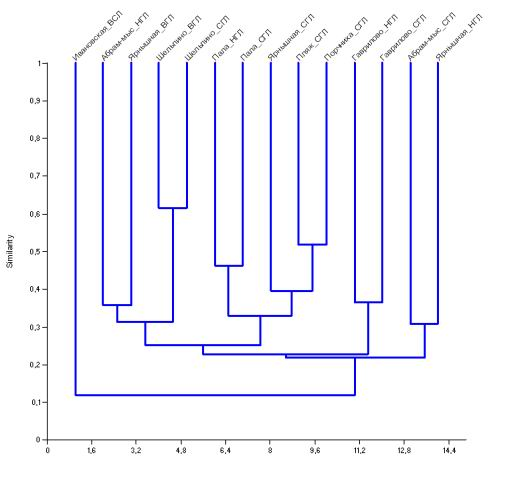
\includegraphics{../Barenc_Sea/soobshestvo/soobshestvo_po_gorizontam_Jakkard_paired_group_clusters.jpg}
		\end{center}
	\caption{Классификация отдельных горизонтов литорали по видовому составу}
	\label{ris:cluster_barents_species_tidal}

	\footnotesize{Кластеризация по методу ближайшего соседа с использованием коэффициента Жаккара. По оси ординат --- коэффициент Жаккара}
	\end{figure}
На еще более низком уровне сходства ($40$\%) выделяется литораль Пала-губы и губы Гаврилово. 

Возможно, что была выбрана слишком дробная единица анализа, и посмотрим как разложаться полные описания сообществ по изученных участкам литорали (рис.~\ref{ris:cluster_barents_species_sites}. 
	\begin{figure}
		\begin{center}
			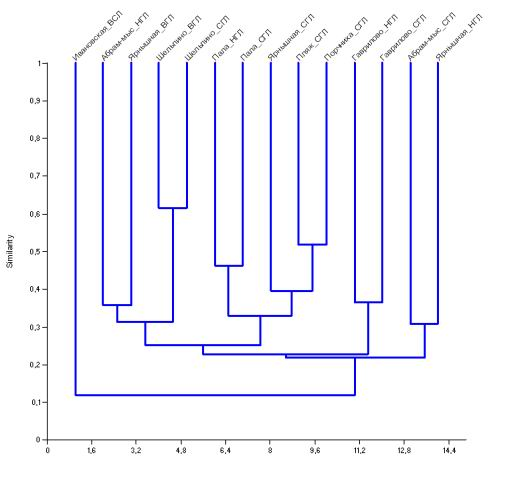
\includegraphics{../Barenc_Sea/soobshestvo/soobshestvo_po_gorizontam_Jakkard_paired_group_clusters.jpg}
		\end{center}
	\caption{Классификация участков по видовому составу}
	\label{ris:cluster_barents_species_sites}

	\footnotesize{Кластеризация по методу ближайшего соседа с использованием коэффициента Жаккара. По оси ординат --- коэффициент Жаккара}
	\end{figure}
На $50$\% уровне сходства было выделено одна группа участков --- губы Ярнышная, Дальнезеленецая и Порчниха.  
На более низком уровне сходства ($40$\%) к первой группе участков добавляется губа Гаврилово, и выделяется вторая группа сходных участков --- Абрам-мыс и губа Шельпино. 
Однако если в первой группе находятся участки, сближенные географически, то во вторую попали участки из разных акваторий.  

Влияние фактора гранулометрического состава грунта на состав сообщества было оценено с помощью анализа сходства ANOSIM. 
Градации фактора были заданы как илисто-песчаная, песчаная и гравийно-песчаная литораль, а в качестве меры сходства использовали коэффициент Жаккара. 
В результате не было обнаружено достоверного влияния данного показателя на видовой состав сообщества ($R=0,053, p=0,36$).
	
Таким образом, таксономический состав сообществ на исследованных участках достаточно вариабелен, и по-видимому, сходство определяется географической близостью участков. 

%была еще тема на конференции в Мурманске. Не надо ли добавить оттуда и пересчитать все нафиг.
 
\afterpage{\clearpage}

%%микрораспределение
\section{Микрораспределение {\it Macoma balthica}}	
Описание микрораспределения макробентоса проводили при помощи метода пространственных автокорреляций с использованием индекса Морана (\cite{Thrush_et_al_1989}).

\subsection{Восточный Мурман}
На Восточном Мурмане в 2007 году были проведены исследования микрораспределения маком на двух учаcтках --- в куту губы Ярнышная (рис.~\ref{ris:MoranI_Yarnyshnaya}) и на Дальнем пляже губы Дальнезеленецкой (рис.~\ref{ris:MoranI_DZ_2007}). 
На обоих участках не было обнаружено пятен агрегации, связанных с распределением моллюсков по численности или биомассе.
%
	\begin{figure}[h]
	\begin{minipage}[b]{.46\linewidth}
	%Фигурка в первом ряду слева размер отведенный под весь этот объект -- 0.46 от ширины строки
	%Параметр [b] означает, что выравнивание этих министраниц будет по нижнему краю
	\begin{center}
	{\small N}\\
	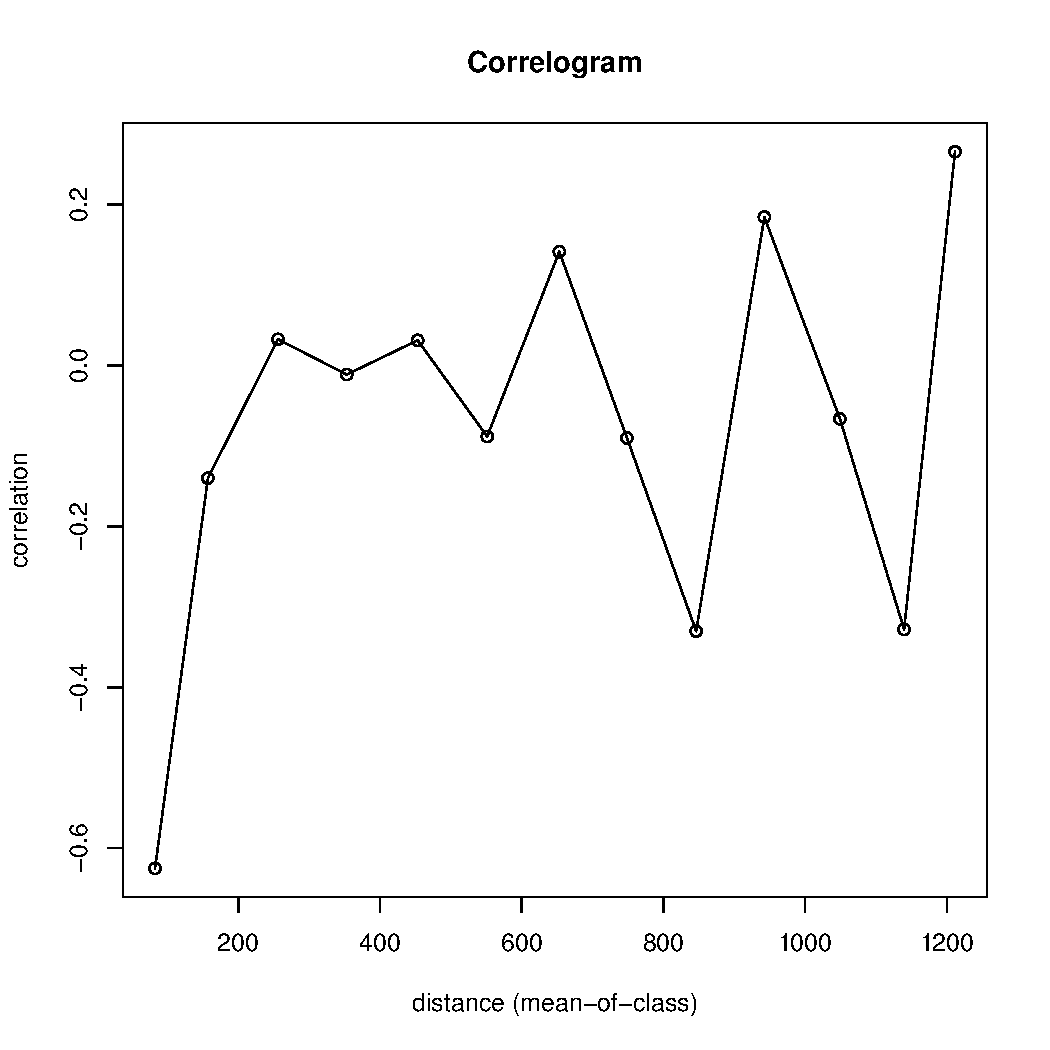
\includegraphics[width=80mm]{../Barenc_Sea/distribution_Moran/Yarnyshnaya07_moran_N_Macoma_balthica_.pdf}
	\end{center}
	\end{minipage}
%
	\hfil %Это пружинка отодвигающая рисунки друг от друга
%
	\begin{minipage}[b]{.46\linewidth}
%Следующий рисунок - первый ряд справа %DUNGEON S_4 \ AB
	\begin{center}
	{\small B}\\
		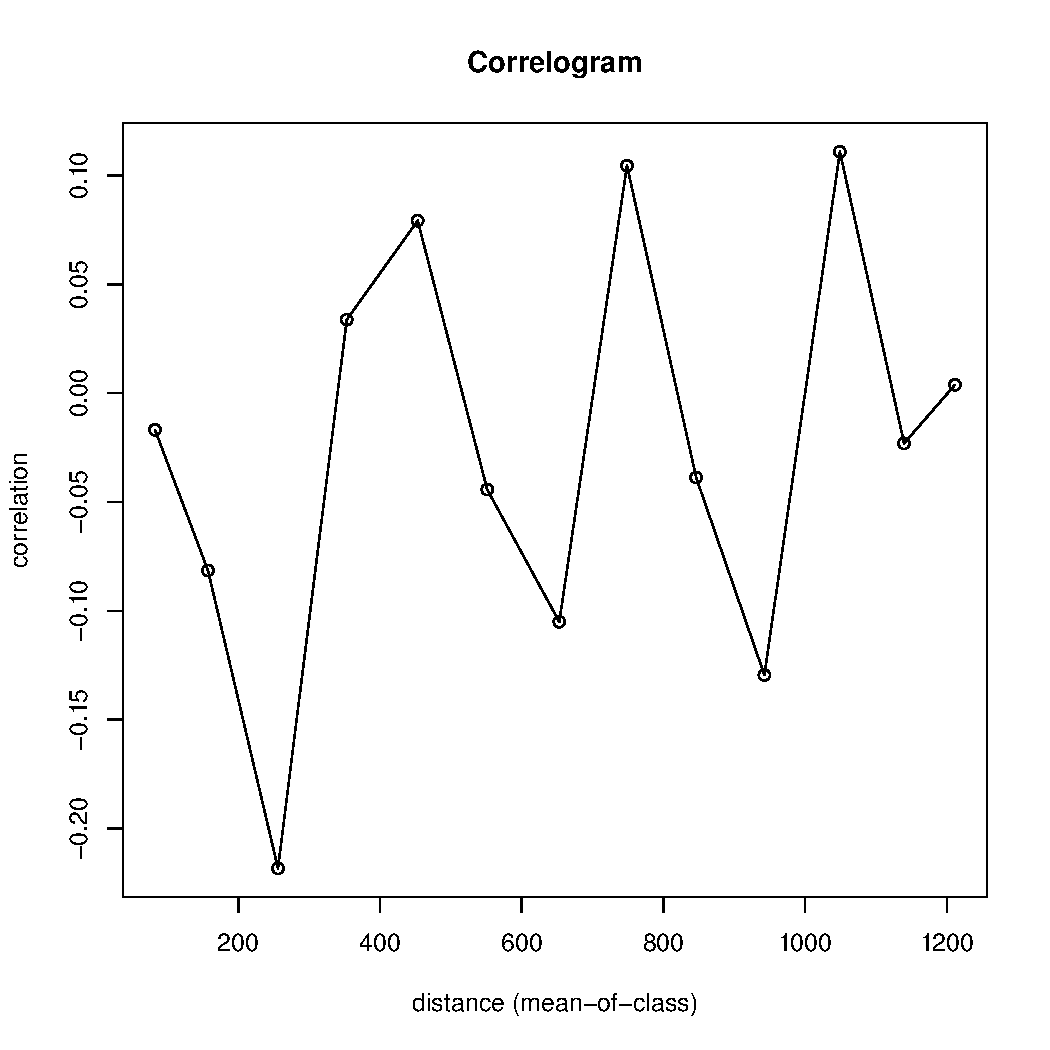
\includegraphics[width=80mm]{../Barenc_Sea/distribution_Moran/Yarnyshnaya07_moran_B_Macoma_balthica_.pdf}
	\end{center}
	\end{minipage}
	
	\begin{minipage}[b]{.46\linewidth}
	%Фигурка в первом ряду слева размер отведенный под весь этот объект -- 0.46 от ширины строки
	%Параметр [b] означает, что выравнивание этих министраниц будет по нижнему краю
	\begin{center}
		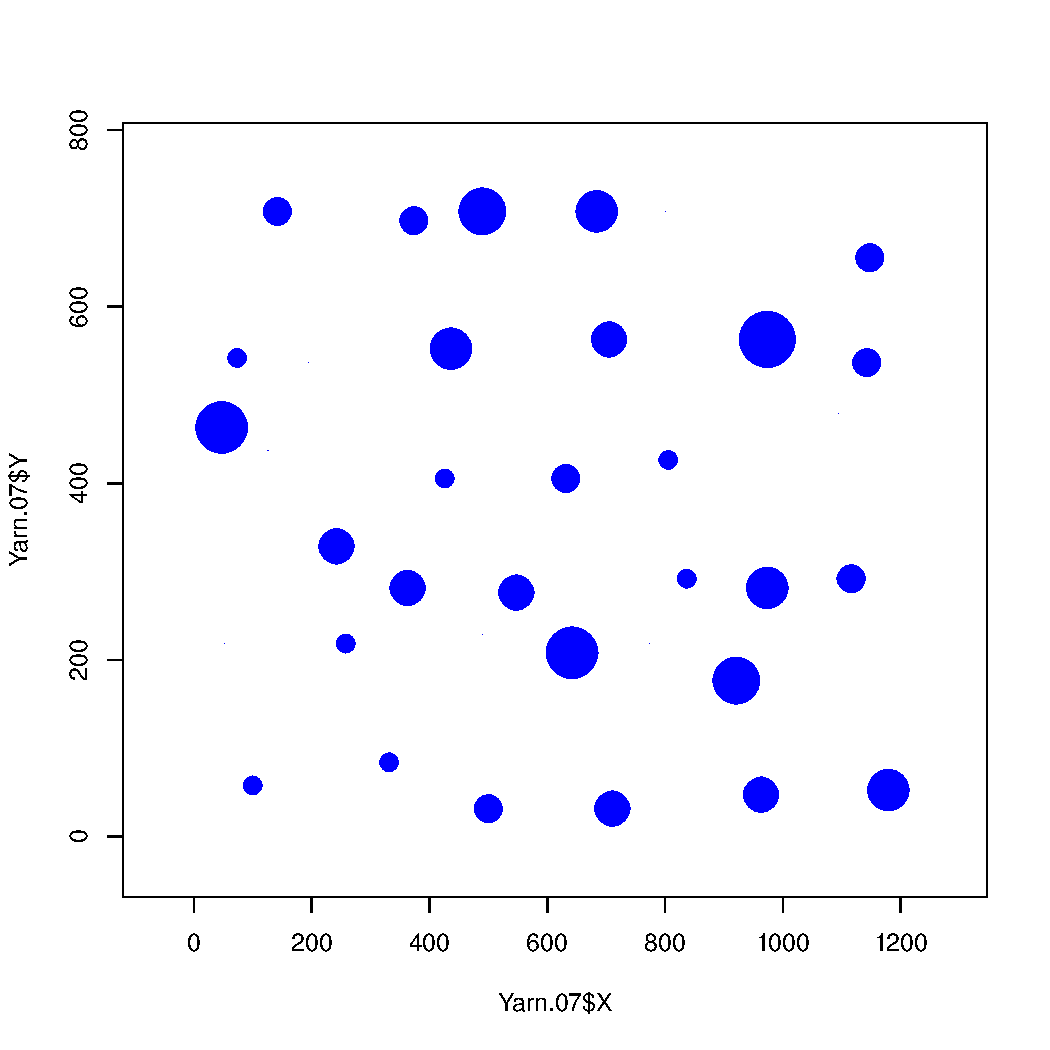
\includegraphics[width=80mm]{../Barenc_Sea/distribution_Moran/Yarnyshnaya_N_Macoma_bubbles.pdf}
	\end{center}
	\end{minipage}
	%
	\hfil %Это пружинка отодвигающая рисунки друг от друга
	%
	\begin{minipage}[b]{.46\linewidth}
%Следующий рисунок - первый ряд справа %DUNGEON S_4 \ AB
	\begin{center}
		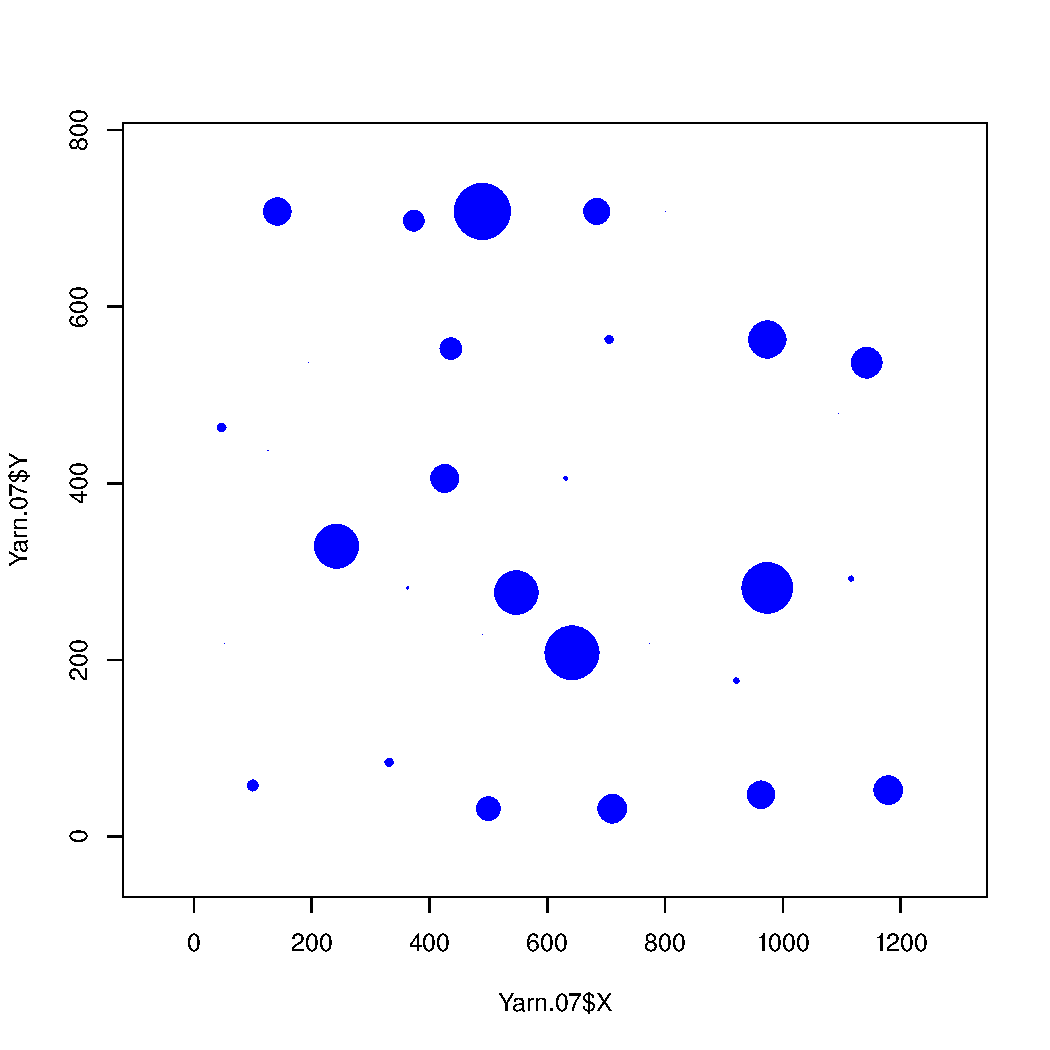
\includegraphics[width=80mm]{../Barenc_Sea/distribution_Moran/Yarnyshnaya_B_Macoma_bubbles.pdf}
	\end{center}
	\end{minipage}
	\caption{Коррелограммы Морана, описывающие микрораспределение, и реальное распределение {\it Macoma balthica} на литорали губы Ярнышная}
	\label{ris:MoranI_Yarnyshnaya}

	\footnotesize{Примечание: N --- распределение особей по численности. B -- распределение особей по биомассе.\\
	Moran's I --- коэффициент пространственной автокорреляции Морана. lag --- расстояние,~см. Закрашенные точки соответстсвуют достоверным значениям коэффициента корреляции ($p \le 0,05$).\\
	На пузырьковых диаграммах площадь кругов пропорциональна обилию маком.}
	\end{figure}



	\begin{figure}[h]

	\begin{minipage}[b]{.46\linewidth}
%Фигурка в первом ряду слева размер отведенный под весь этот объект -- 0.46 от ширины строки
%Параметр [b] означает, что выравнивание этих министраниц будет по нижнему краю
	\begin{center}
	{\small N}\\
		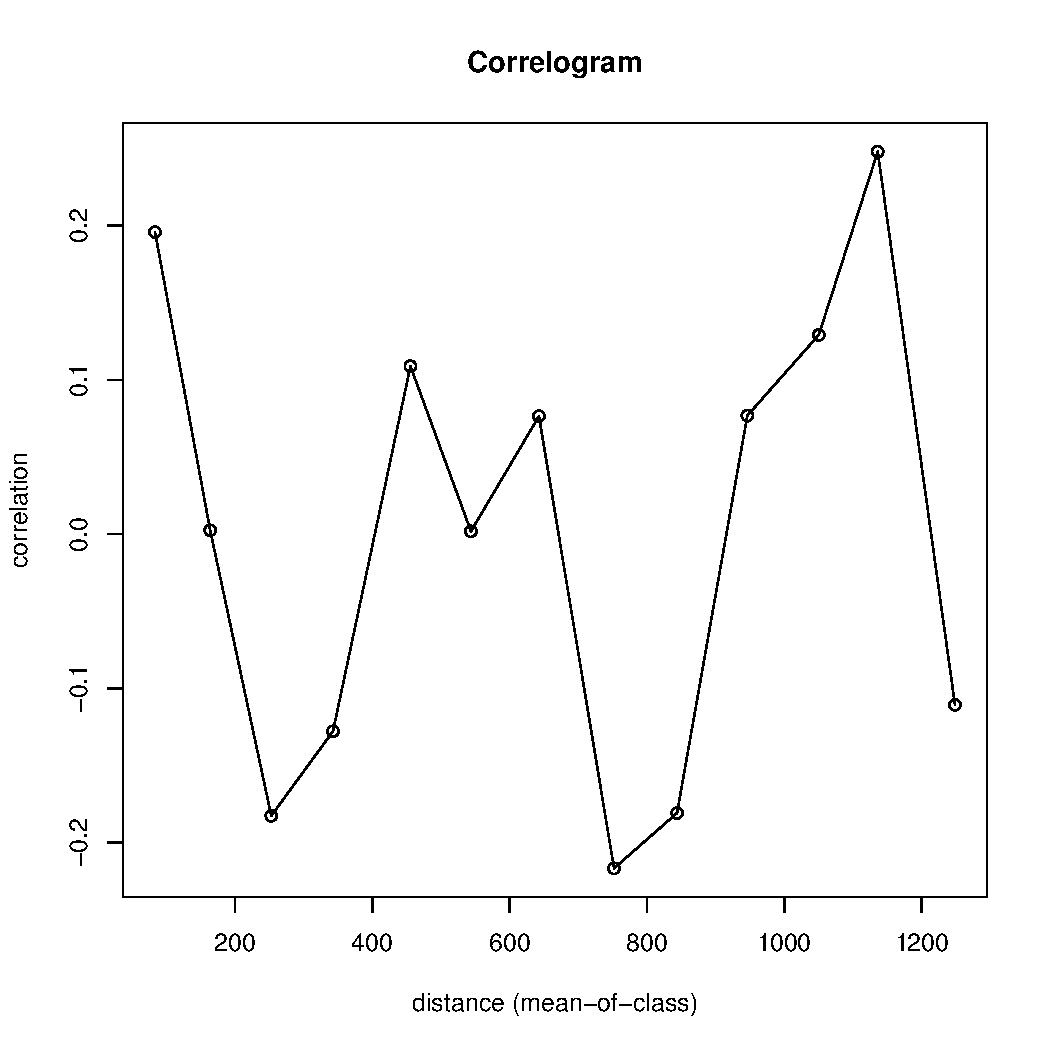
\includegraphics[width=80mm]{../Barenc_Sea/distribution_Moran/Plyazh07_moran_N_Macoma_balthica_.pdf}
	\end{center}
	\end{minipage}
%
	\hfil %Это пружинка отодвигающая рисунки друг от друга
%
	\begin{minipage}[b]{.46\linewidth}
%Следующий рисунок - первый ряд справа %DUNGEON S_4 \ AB
	\begin{center}
	{\small B}\\
		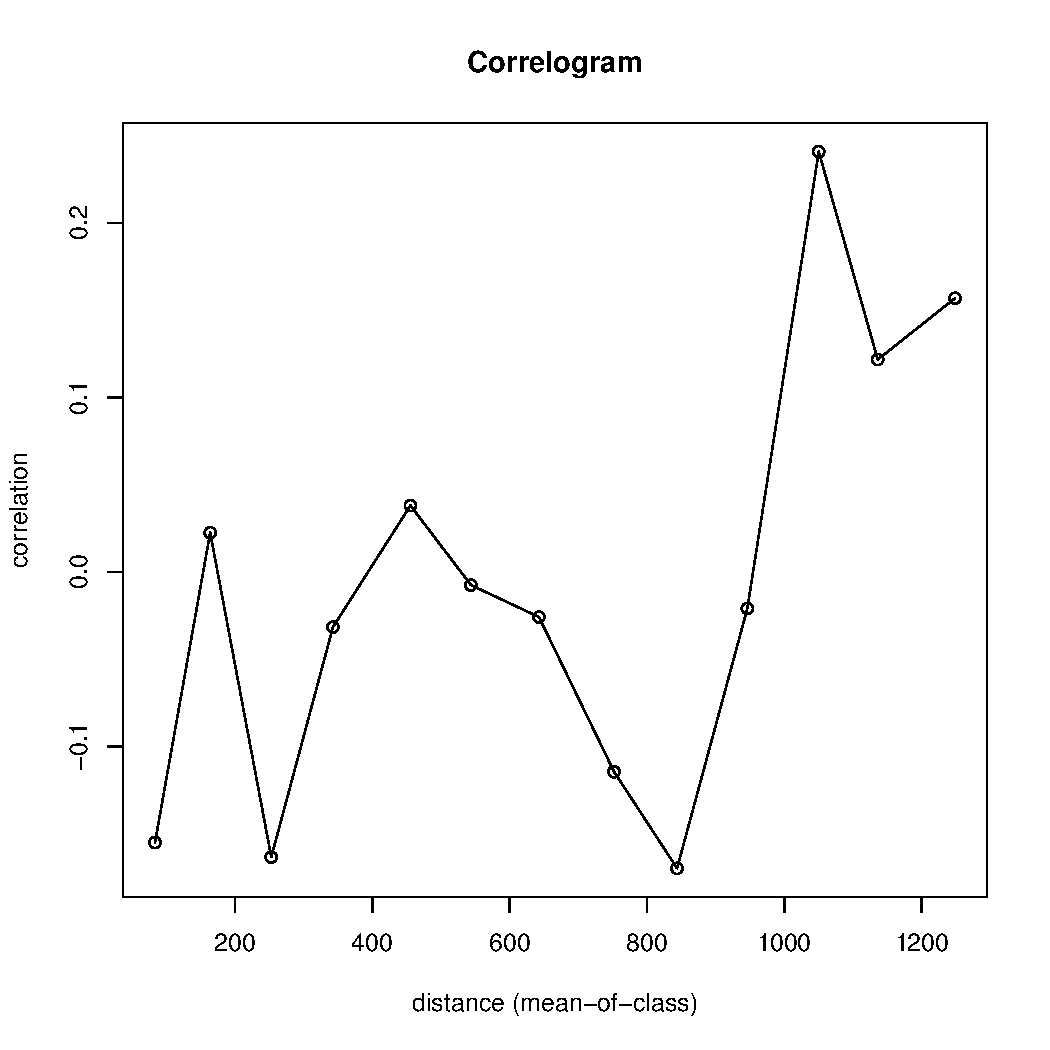
\includegraphics[width=80mm]{../Barenc_Sea/distribution_Moran/Plyazh07_moran_B_Macoma_balthica_.pdf}
	\end{center}
	\end{minipage}
	
	\begin{minipage}[b]{.46\linewidth}
	%Фигурка в первом ряду слева размер отведенный под весь этот объект -- 0.46 от ширины строки
	%Параметр [b] означает, что выравнивание этих министраниц будет по нижнему краю
	\begin{center}
		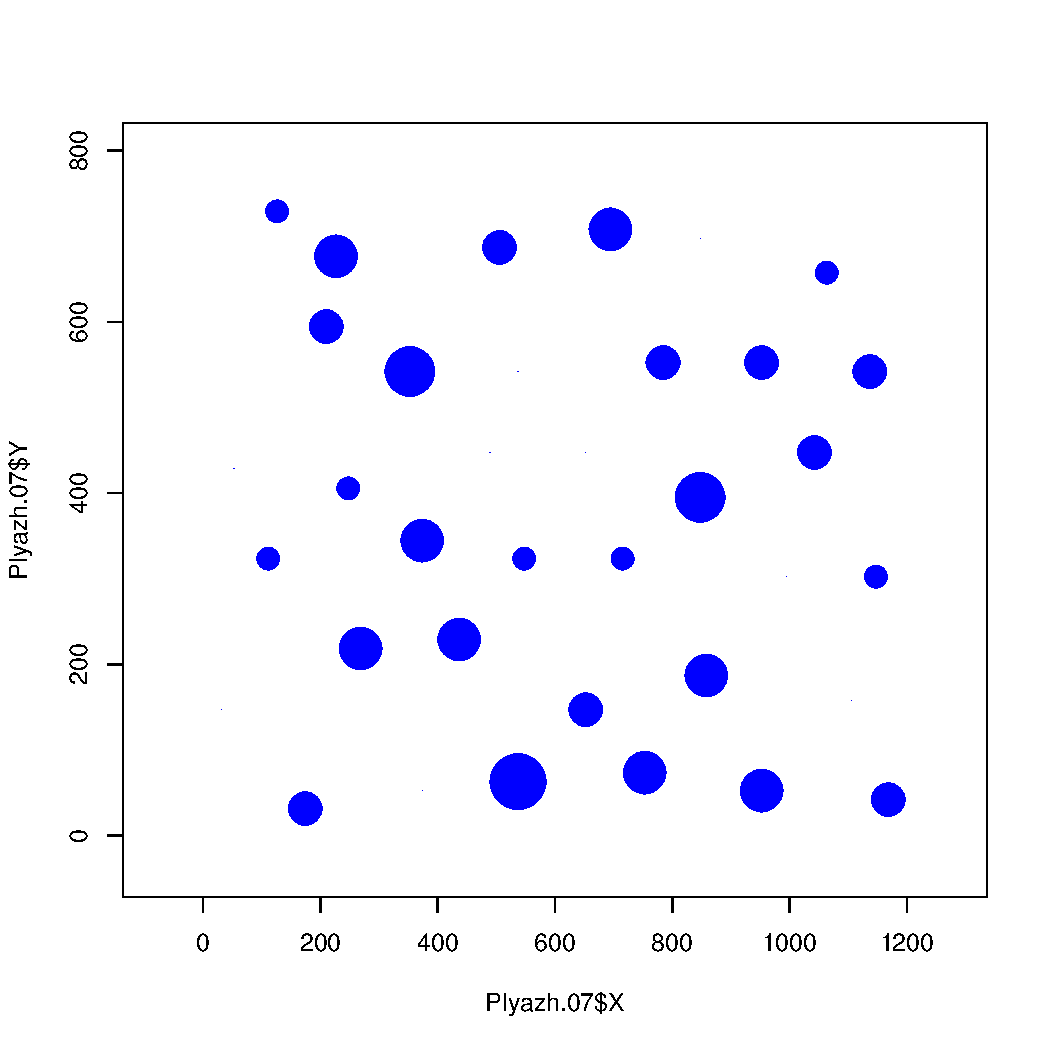
\includegraphics[width=80mm]{../Barenc_Sea/distribution_Moran/Plyazh07_N_Macoma_bubbles.pdf}
	\end{center}
	\end{minipage}
	%
	\hfil %Это пружинка отодвигающая рисунки друг от друга
	%
	\begin{minipage}[b]{.46\linewidth}
%Следующий рисунок - первый ряд справа %DUNGEON S_4 \ AB
	\begin{center}
		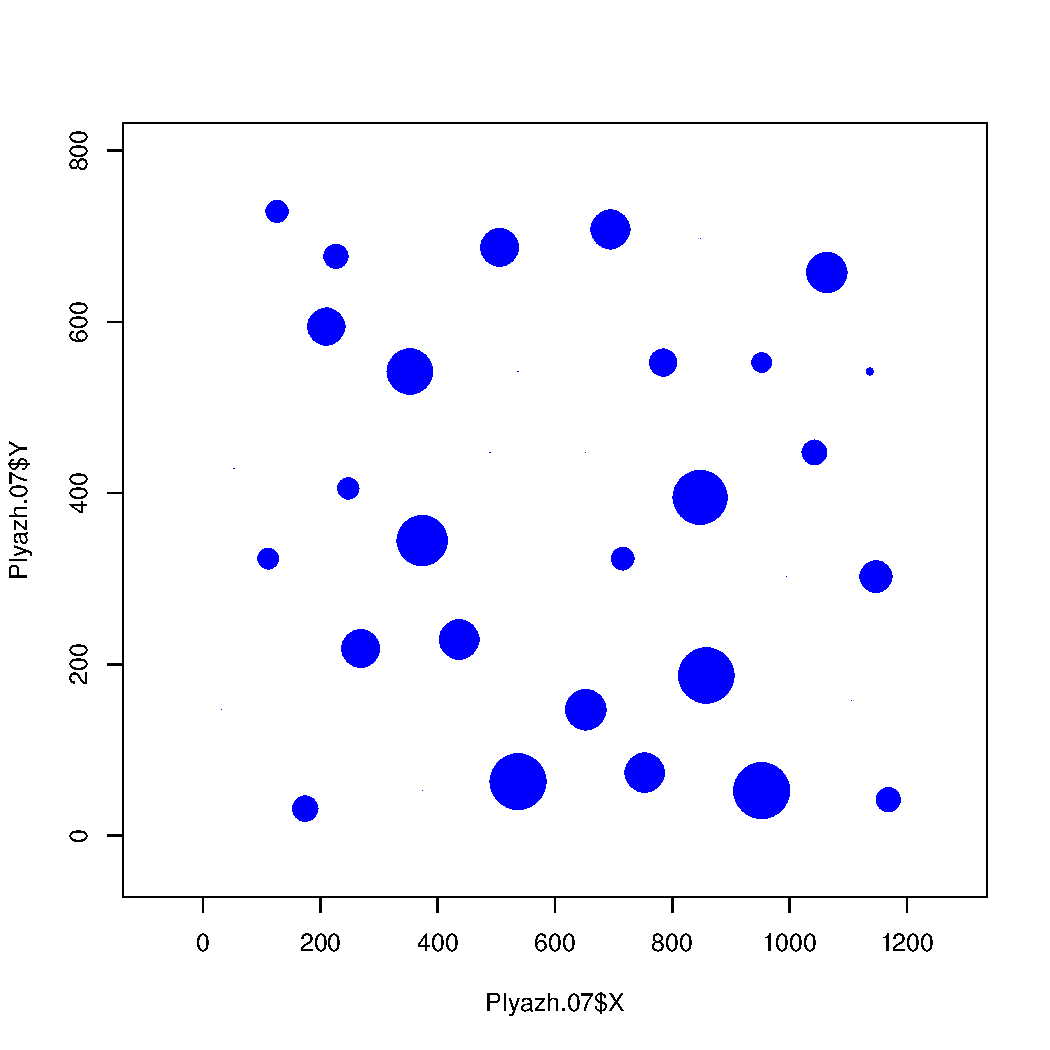
\includegraphics[width=80mm]{../Barenc_Sea/distribution_Moran/Plyazh07_B_Macoma_bubbles.pdf}
	\end{center}
	\end{minipage}
	\caption{Коррелограммы Морана, описывающие микрораспределение, и реальное распределение {\it Macoma balthica} на литорали губы Дальнезеленецкая в 2007 году}
	\label{ris:MoranI_DZ_2007}

	\footnotesize{Примечание: N --- распределение особей по численности. B -- распределение особей по биомассе.\\
	Moran's I --- коэффициент пространственной автокорреляции Морана. lag --- расстояние,~см. Закрашенные точки соответстсвуют достоверным значениям коэффициента корреляции ($p \le 0,05$).\\
	На пузырьковых диаграммах площадь кругов пропорциональна обилию маком.}
	\end{figure}

Мы предположили, что размер учетного полигона слишком маленький для выявления особенностей распределения, и в 2008 году повторили съемку, увеличив размер полигона и количество проб в два раза.
Достоверные значения коэффициента простарнственной корреляции Морана были показаны для расстояний около $1,5-2$~м (отрицательный) и на расстоянии около $4$~м (положительный) (рис.~\ref{ris:MoranI_DZ_2008}).
%
	\begin{figure}[h]

	\begin{minipage}[b]{.46\linewidth}
%Фигурка в первом ряду слева размер отведенный под весь этот объект -- 0.46 от ширины строки
%Параметр [b] означает, что выравнивание этих министраниц будет по нижнему краю
	\begin{center}
	{\small N}\\
		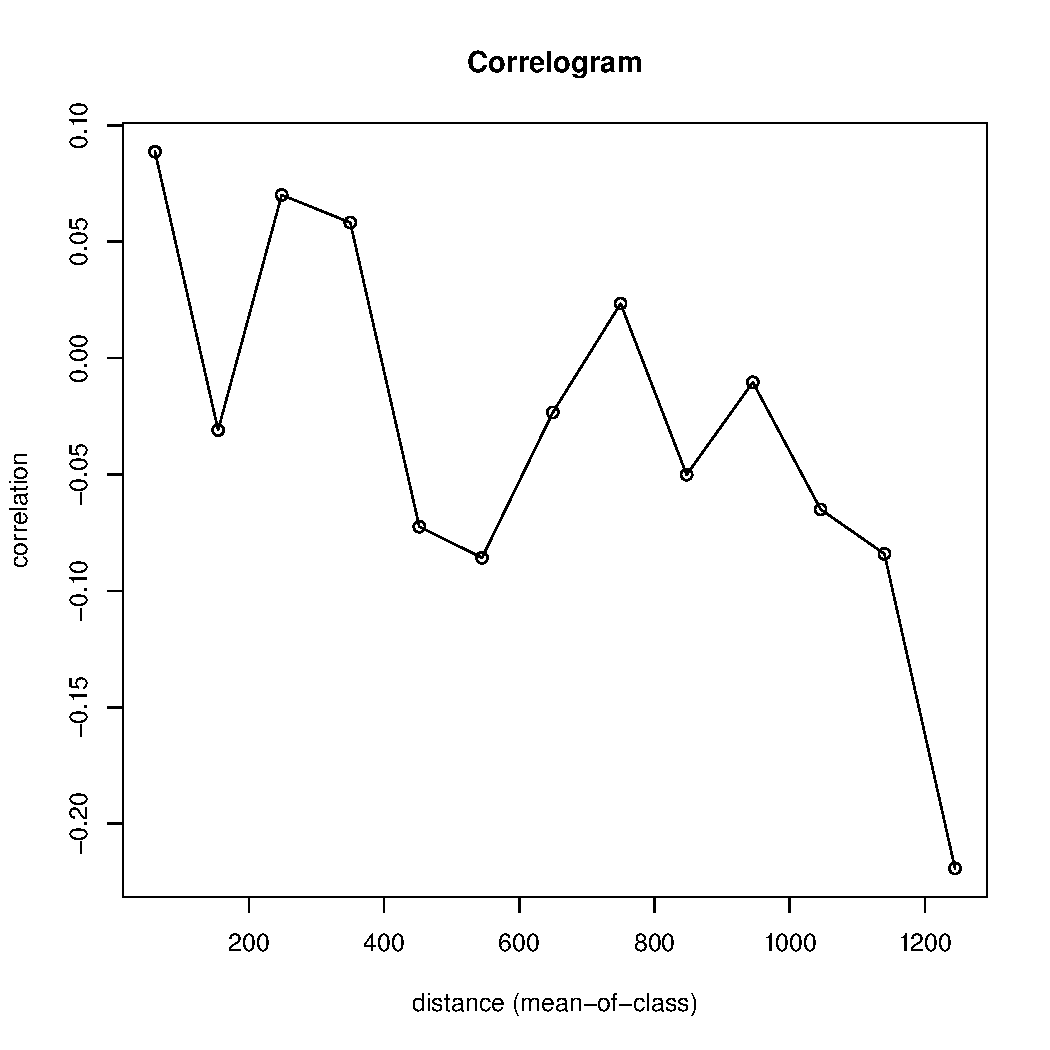
\includegraphics[width=80mm]{../Barenc_Sea/distribution_Moran/Plyazh0812_moran_N_Macoma_balthica_.pdf}
	\end{center}
	\end{minipage}
%
	\hfil %Это пружинка отодвигающая рисунки друг от друга
%
	\begin{minipage}[b]{.46\linewidth}
%Следующий рисунок - первый ряд справа %DUNGEON S_4 \ AB
	\begin{center}
	{\small B}\\
		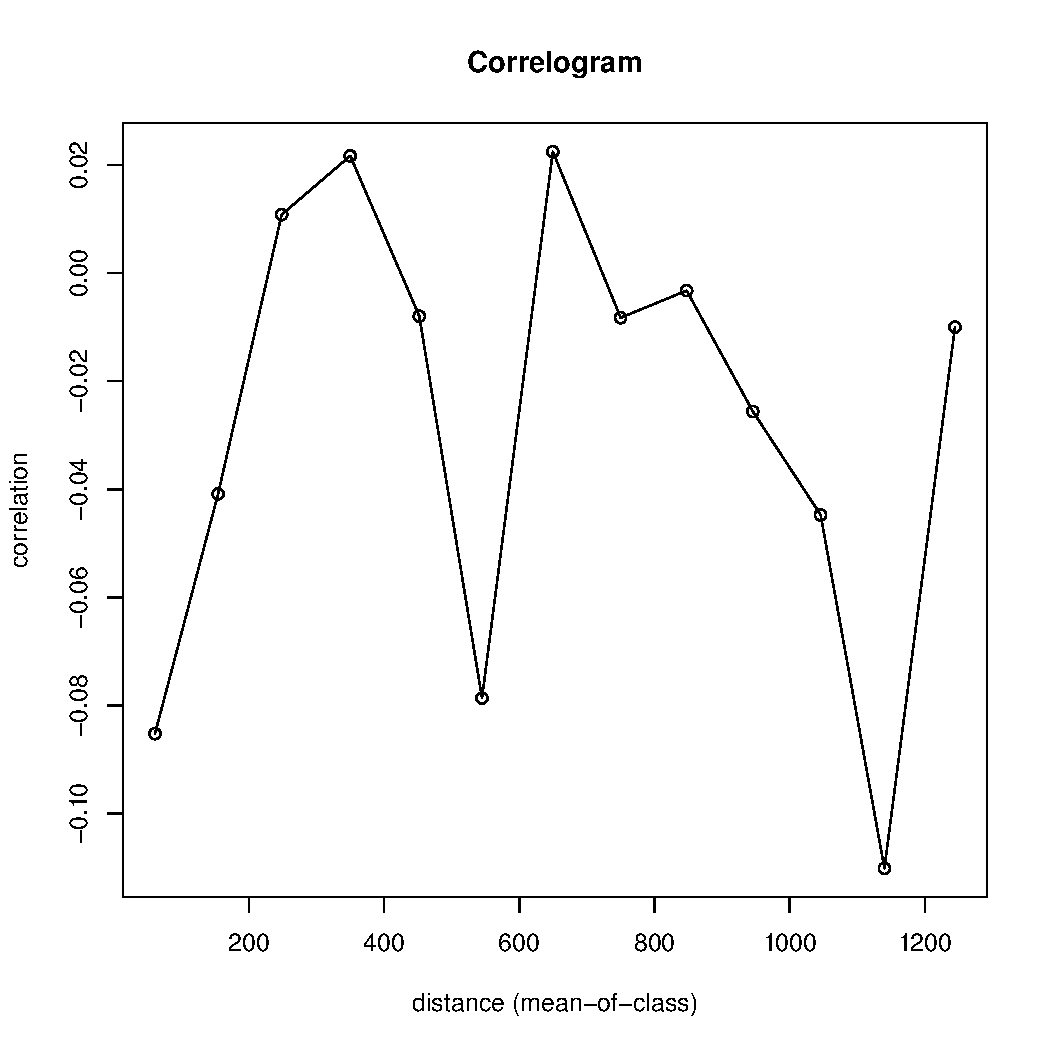
\includegraphics[width=80mm]{../Barenc_Sea/distribution_Moran/Plyazh0812_moran_B_Macoma_balthica_.pdf}
	\end{center}
	\end{minipage}
	
	\begin{minipage}[b]{.46\linewidth}
	%Фигурка в первом ряду слева размер отведенный под весь этот объект -- 0.46 от ширины строки
	%Параметр [b] означает, что выравнивание этих министраниц будет по нижнему краю
	\begin{center}
		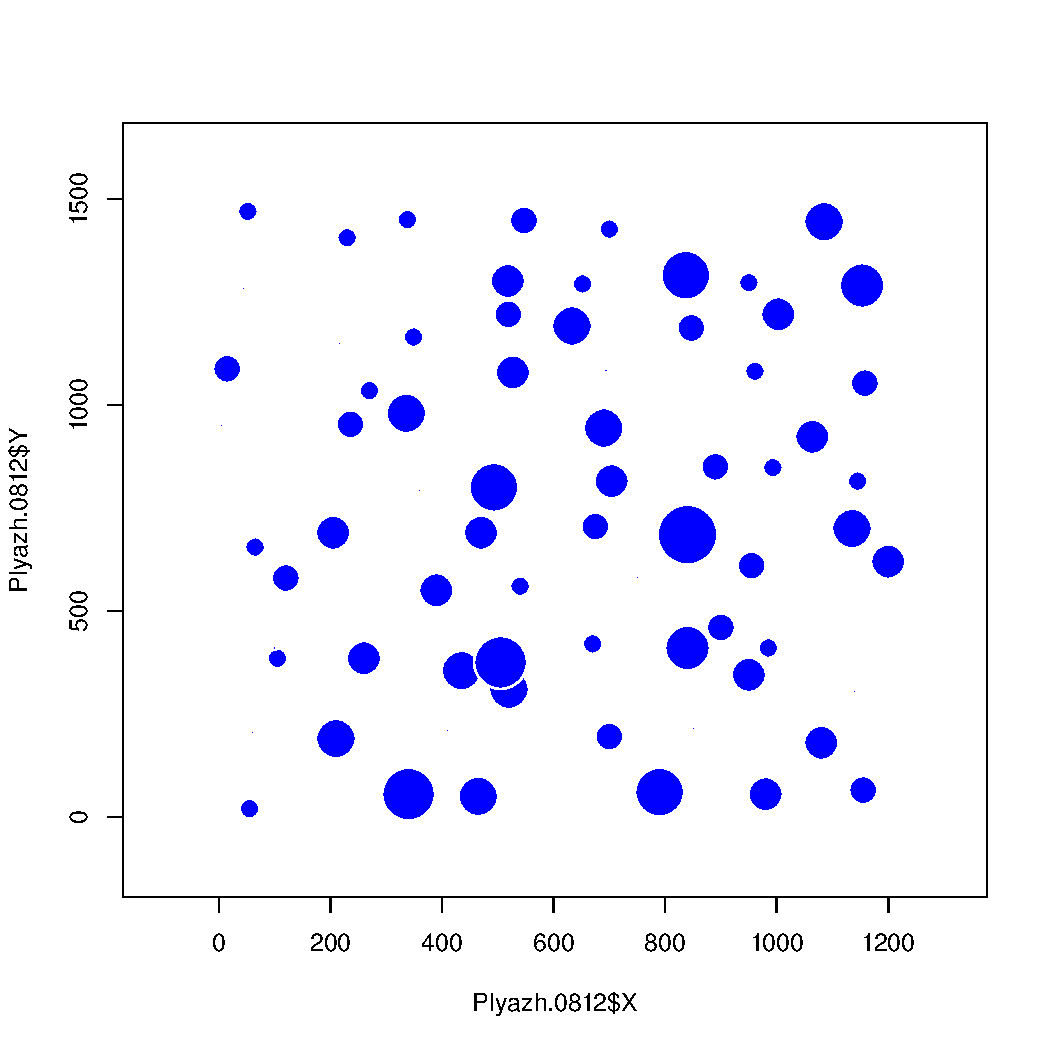
\includegraphics[width=80mm]{../Barenc_Sea/distribution_Moran/Plyazh0812_N_Macoma_bubbles.pdf}
	\end{center}
	\end{minipage}
	%
	\hfil %Это пружинка отодвигающая рисунки друг от друга
	%
	\begin{minipage}[b]{.46\linewidth}
%Следующий рисунок - первый ряд справа %DUNGEON S_4 \ AB
	\begin{center}
		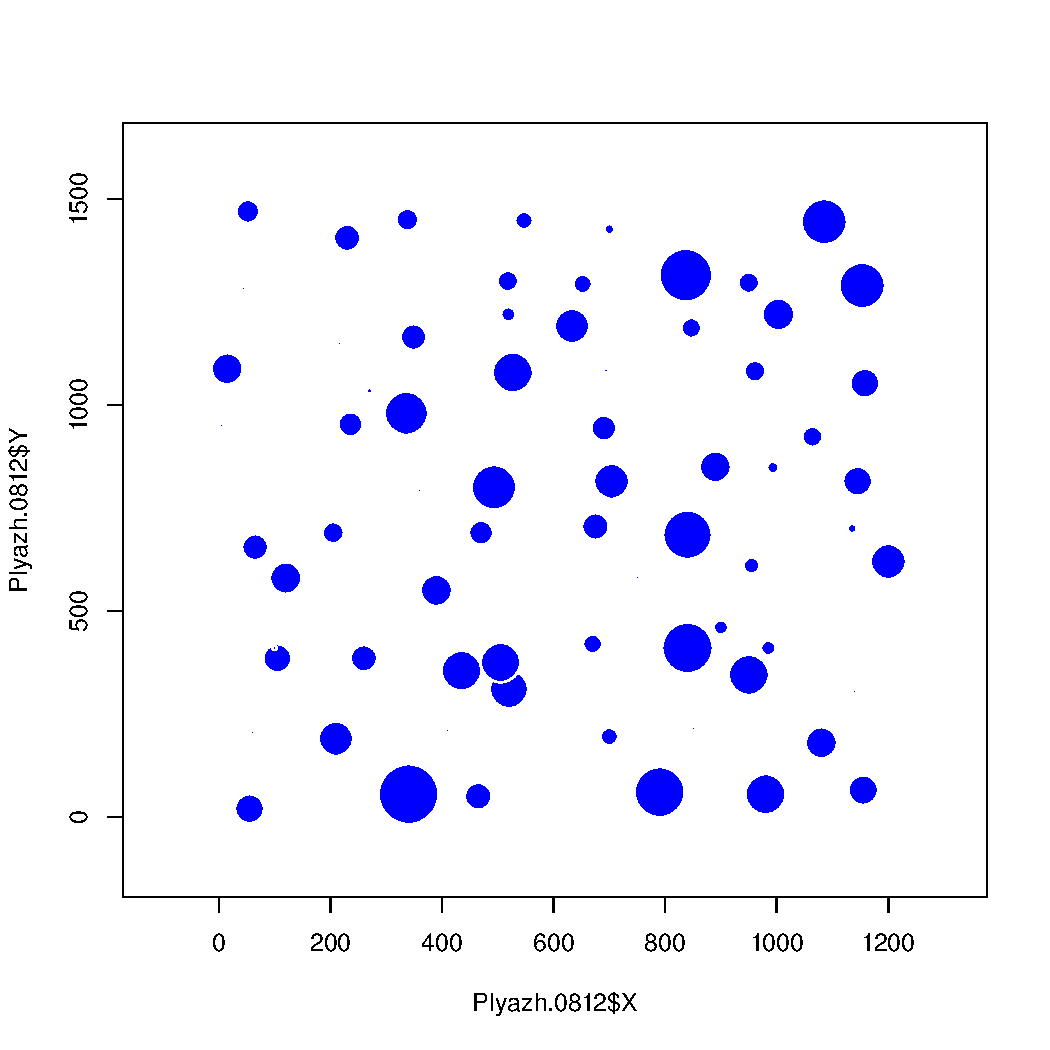
\includegraphics[width=80mm]{../Barenc_Sea/distribution_Moran/Plyazh0812_B_Macoma_bubbles.pdf}
	\end{center}
	\end{minipage}
	\caption{Коррелограммы Морана, описывающие микрораспределение, и реальное распределение {\it Macoma balthica} на литорали губы Дальнезеленецкая в 2008 году}
	\label{ris:MoranI_DZ_2008}

	\footnotesize{Примечание: N --- распределение особей по численности. B -- распределение особей по биомассе.\\
	Moran's I --- коэффициент пространственной автокорреляции Морана. lag --- расстояние,~см. Закрашенные точки соответстсвуют достоверным значениям коэффициента корреляции ($p \le 0,05$).\\
	На пузырьковых диаграммах площадь кругов пропорциональна обилию маком.}
	\end{figure}
%
Это позволяет предположить сложную структуру пространственного распределения особей: локальные агрегации, сравнимые по размеру с размером учетной рамки (1/30 м$^2$), организованные в более крупные скопления. 


	\subsection{Кольский залив}
На литорали Пала-губы особи {\it M.~balthica} формируют скопления размером около $2-4$~м (рис.~\ref{ris:moransI_Pala_Macoma}). 
Наличие серии достоверно отрицательных значений индекса автокорреляции Морана для больших расстояний свидетельствует о наличии либо градиентого изменения численности, либо крупной агрегации с нечеткими краями.
Наличие градиентного изменения обилия в направлении к руслу ручья было показано с использованием коэффициента корреляции Кендалла ($\tau = 0,55; p = 3,48 \times 10^{-6}$).
Распределение маком по биомассе соответствует распределению по численности (рис.~\ref{ris:moransI_Pala_Macoma}). Также корреляционный анализ Кендалла показал градиентное уменьшение биомассы в направлении от моря ($\tau = -0,4; p = 0,0005$).
	\begin{figure}[h]

	\begin{minipage}[b]{.5\linewidth}
	%Фигурка в первом ряду слева размер отведенный под весь этот объект -- 0.46 от ширины строки
	%Параметр [b] означает, что выравнивание этих министраниц будет по нижнему краю
	\begin{center}
	{\small N}\\
		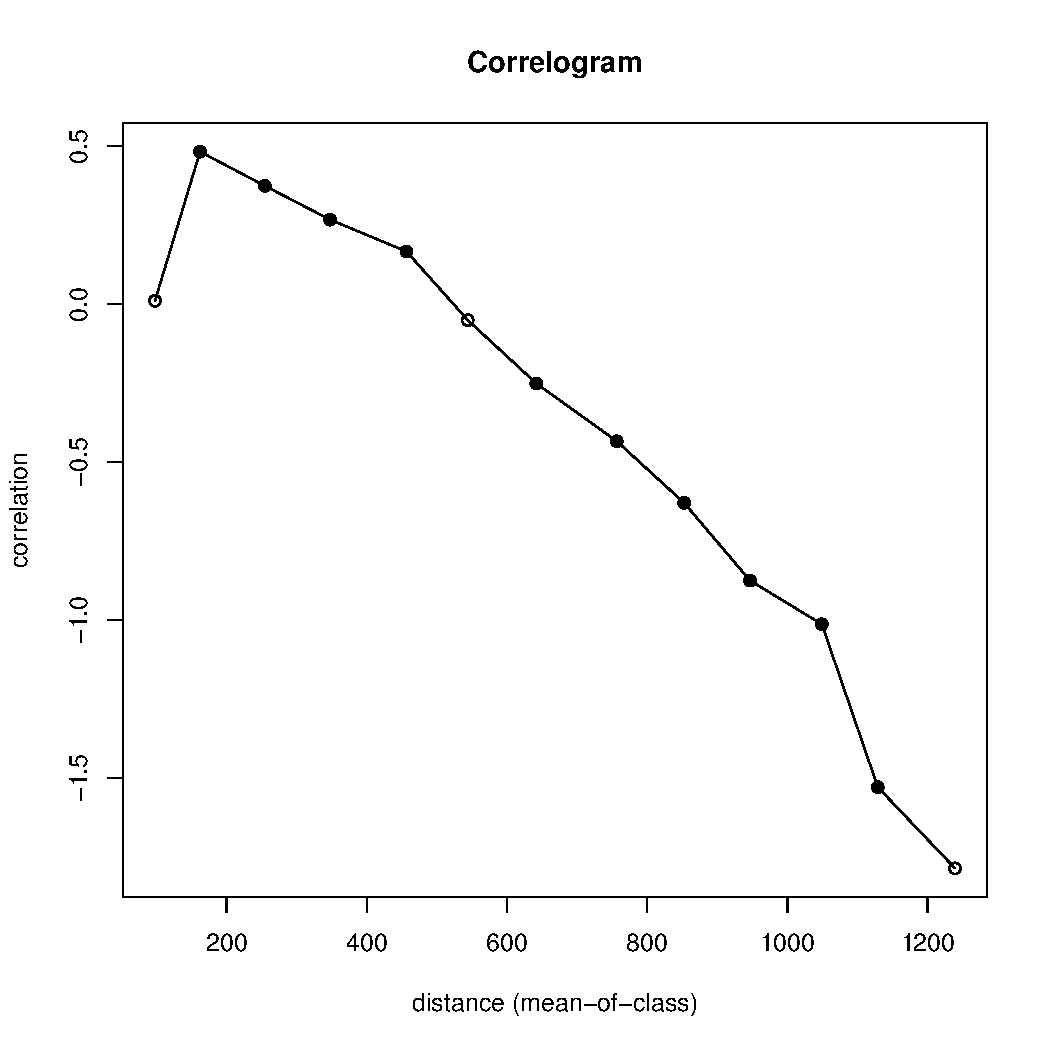
\includegraphics[width=80mm]{../Barenc_Sea/distribution_Moran/Pala_moran_N_Macoma_balthica_.pdf}
	\end{center}
	\end{minipage}
	%
	\hfil %Это пружинка отодвигающая рисунки друг от друга
	%
	\begin{minipage}[b]{.5\linewidth}
	%Следующий рисунок - первый ряд справа %DUNGEON S_4 \ AB
	\begin{center}
	{\small B}\\
		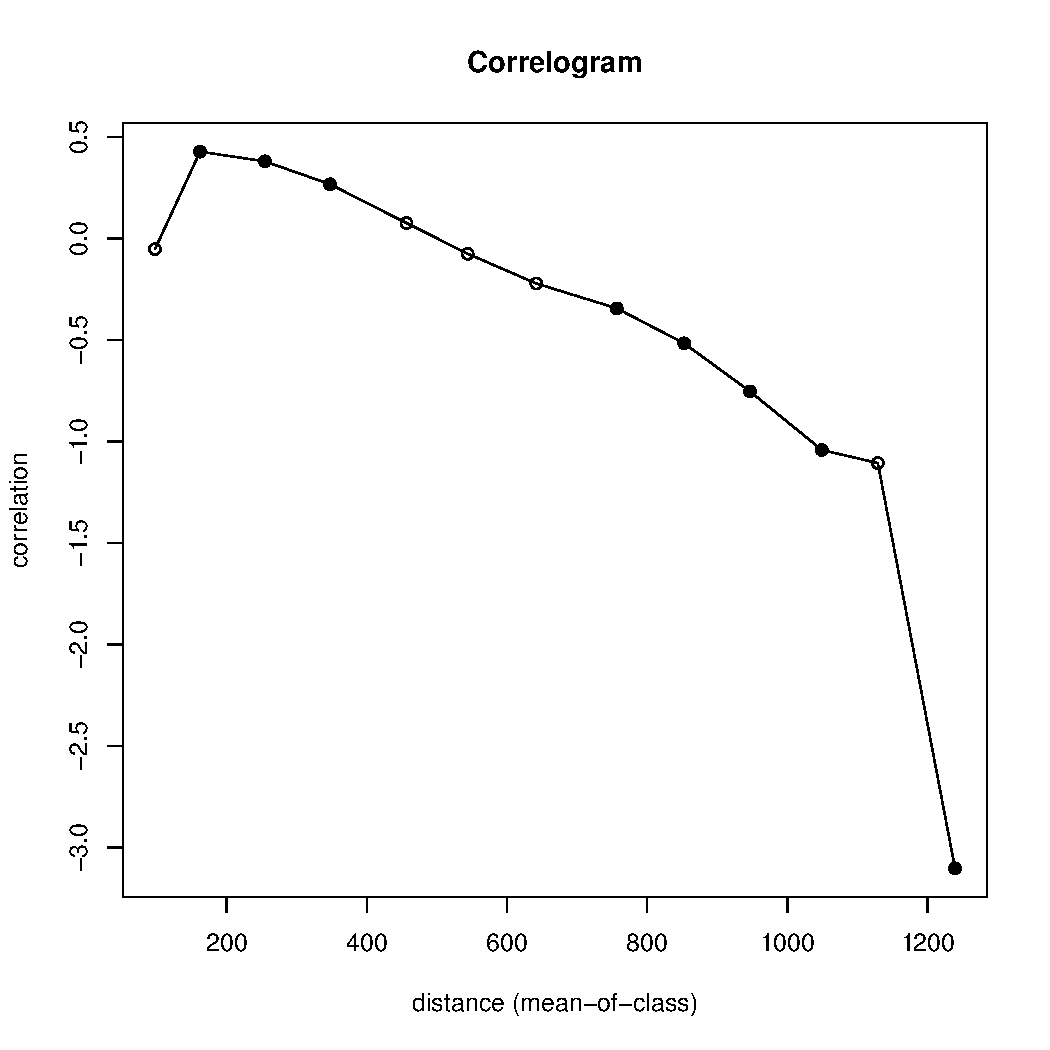
\includegraphics[width=80mm]{../Barenc_Sea/distribution_Moran/Pala_moran_B_Macoma_balthica_.pdf}
	\end{center}
	\end{minipage}

	\begin{minipage}[b]{.5\linewidth}
	\begin{center}
		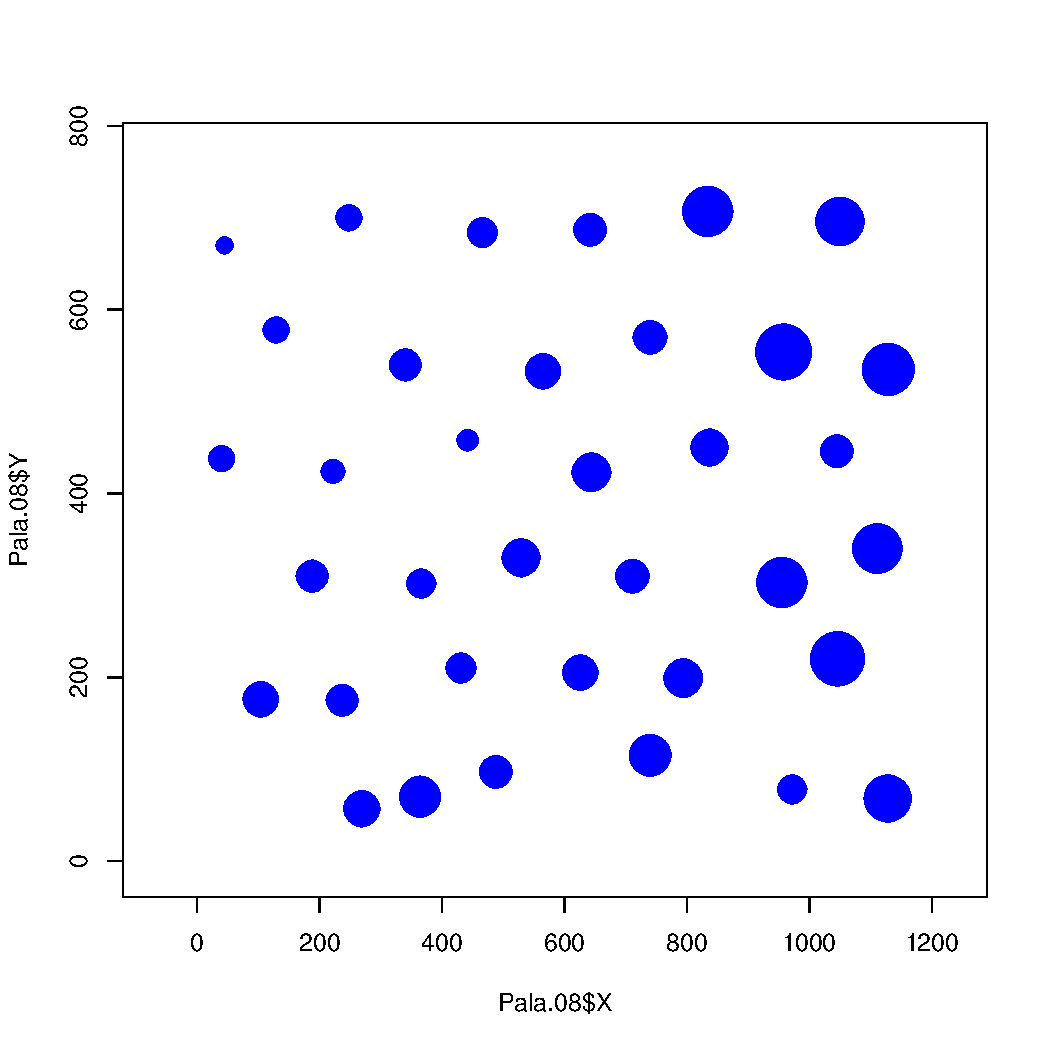
\includegraphics[width=80mm]{../Barenc_Sea/distribution_Moran/Pala_N_Macoma_bubbles.pdf}
	\end{center}
	\end{minipage}
	%
	\hfil %Это пружинка отодвигающая рисунки друг от друга
	%
	\begin{minipage}[b]{.5\linewidth}
	%Следующий рисунок - первый ряд справа %DUNGEON S_4 \ AB
	\begin{center}
		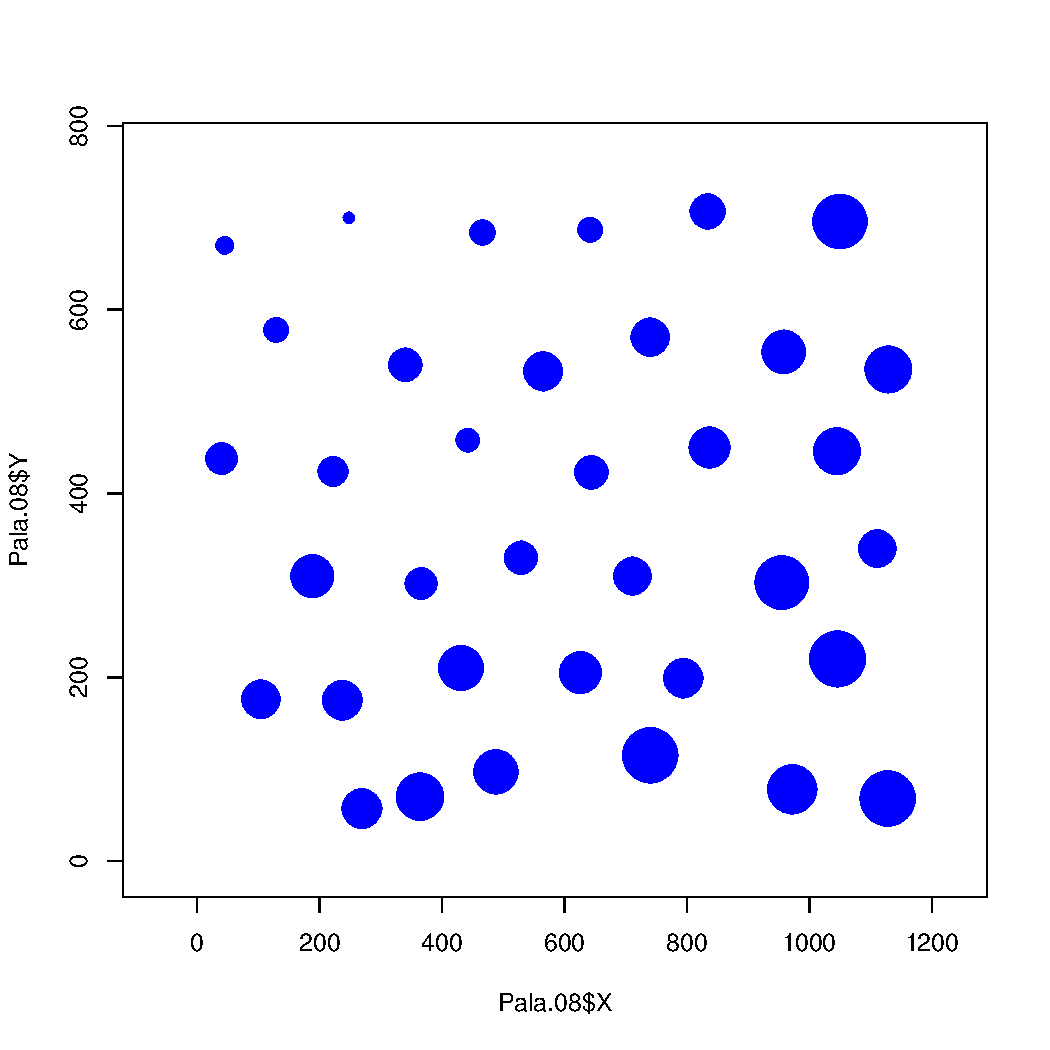
\includegraphics[width=80mm]{../Barenc_Sea/distribution_Moran/Pala_B_Macoma_bubbles.pdf}
	\end{center}
	\end{minipage}
	\caption{Коррелограммы Морана, описывающие микрораспределение, и реальное распределение {\it Macoma balthica} на литорали Пала-губы}
	\label{ris:moransI_Pala_Macoma}

	\footnotesize{Примечание: N --- распределение особей по численности. B -- распределение особей по биомассе.\\
	Moran's I --- коэффициент пространственной автокорреляции Морана. lag --- расстояние,~см. Закрашенные точки соответстсвуют достоверным значениям коэффициента корреляции ($p \le 0,05$).\\
	На пузырьковых диаграммах площадь кругов пропорциональна обилию маком.}
	\end{figure}

Поскольку на данном участке обилие маком было достаточно высокое (рис.~\ref{ris:age_Pala_2007_low}), мы отдельно рассмотрели распределение особей разных возрастов.
%
	\begin{figure}[h]
		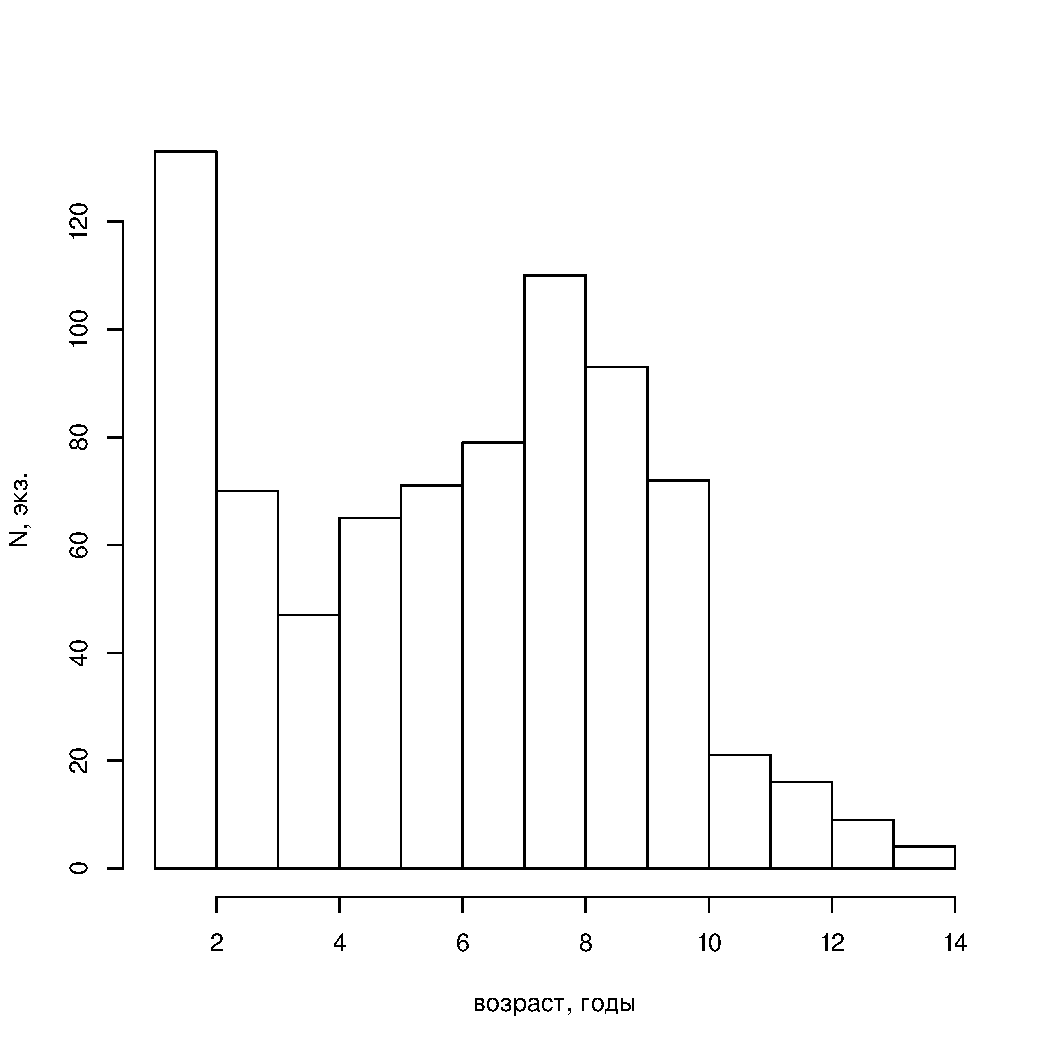
\includegraphics{../Barenc_Sea/Pala/Pala_2007_low_age_hist.pdf}
		\caption{Распределение по возрастам особей {\it Macoma balthica} в пробах на литорали Пала-губы}
		\label{ris:age_Pala_2007_low}
	\end{figure}
%
Коррелограммы Морана и пузырьковые диаграммы, описывающие реальное распределение особей, представлены в приложении \ref{app:Pala_MoranI_ages}.
Было показано, что горизонтальный градиент общего обилия связан в первую очередь с таким распределением особей возрастом 2, 3 и 5 лет (табл.~\ref{tab:Pala_ages_distribution}). 
%
\begin{table}[h]
		\caption{Пространственное распределение особей {\it Macoma balthica} разного возраста}
		\label{tab:Pala_ages_distribution}
\begin{tabularx}{\linewidth}{|c|X|rr|rr|}
\hline
	& распределение		& \multicolumn{2}{c|}{градиент горизонтальный} & \multicolumn{2}{c|}{градиент вертикальный}   \\ \cline{3-6}
возраст  &  по результатам пространственной автокорреляции  & $Kendall\ \tau$ & $p-value$ & $Kendall\ \tau$ & $p-value$				\\ \hline

1+       & случайное                      & $0,2$	&	$0,17$	&	$0,02$	&	$0,9$                            \\
2+       & градиент                       & $0,45$	&	$0,0003$ ***	&	$0,2$	&	$0,07$ **                   \\
3+       & градиент                       & $0,5$	&	$2,4 \times 10^{-5}$ ***	&	$0,3$	&	$0,002$ ***		 \\
4+       & случайное                      & $0,2$	&	$0,07$ **	&	$0,06$	&	$0,6$                            \\
5+       & градиент                       & $0,43$	&	$0,0005$ ***	&	$-0,02$	&	$0,9$                    \\
6+       & случайное                      & $0,2$	&	$0,03$ ***	&	$-0,03$	&	$0,8$                            \\
7+       & одно большое пятно             & $0,02$	&	$0,9$	&	$-0,02$	&	$0,9$                             \\
8+       & одно большое пятно             & $0,3$	&	$0,01$ ***	&	$-0,2$	&	$0,04$ ***                            \\
9+       & одно большое пятно             & $0,3$	&	$0,01$ ***	&	$-0,2$	&	$0,1$                             \\
10+      & агрегации размером 1 и 3 метра & $0,2$	&	$0,1$	&	$-0,2$	&	$0,08$ **                            \\
11+      & одно большое пятно             & $0,26$	&	$0,053$ **	&	$-0,1$	&	$0,3$                             \\
12+      & агрегации размером 6 метров    & $0,1$	&	$0,3$	&	$-0,2$	&	$0,2$                             \\
13+      & случайное                      & $0,1$	&	$0,4$	&	$0,04$	&	$0,7$                              \\
14+      & случайное                      &  $0,09$	&	$0,5$	&	$-0,15$	&	$0,3$                             \\ \hline
	\end{tabularx}
\end{table}
%
Предположения о градиентном распределении особей данных возрастов, полученных в ходе анализа пространственных автокорреляций Морана подтвердились при корреляционном анализе Кендалла (табл.~\ref{tab:Pala_ages_distribution}).
Однако в нескольких случаях, где коррелограммы Морана не показывают градиентного распределения, анализ Кендалла показывает достоверную корреляцию обилия с координатами. 
Однако во всех случаях речь идет о слабой связи (коэффициент корреляции $0,2$).

Резюмируя полученные данные, можно говорить о большем влиянии ручья на более молодых моллюсков.
Особи старших возрастов формируют агрегации размером в несколько метров.
Наиболее старые моллюски остаются в количестве единичных особей и распределены случайно.


\afterpage{\clearpage}

%%популяционная структура

	\section{Численность {\it Macoma balthica}}
	\subsection{Белое море}
Данные по обилию маком в Кандалакшском заливе Белого моря получены для $10$ участков, всего 140 пространственно-временных точек оценки.
Средняя численность {\it M.~balthica} была представлена в диапазоне от $10$ (о.~Горелый) до $8500$~экз./м$^2$(Западная Ряшкова салма) (табл. \ref{tab:mean_N_White}).
	\begin{footnotesize}
	\begin{longtable}{|p{2cm}|p{3cm}|p{1cm}|p{2cm}|p{1.5cm}|p{1cm}|*{3}{c|}}
	\caption{Средняя численность {\it Macoma balthica} на различных участках Белого моря}\label{tab:mean_N_White}\\
	\hline
	Район & Участок & год & ма\-ре\-ографи\-ческий уровень & число повторностей & площадь учета & $N$, экз./м$^2$ & $S_x$  & $D, \%$ 
	\\ \hline \endfirsthead
	\hline
	\multicolumn{9}{|c|}{продолжение таблицы \ref{tab:mean_N_White}} \\ \hline
	Район & Участок & год & ма\-ре\-ографи\-ческий уровень & число повторностей & площадь учета & $N$, экз./м$^2$ & $S_x$  & $D, \%$ 
	\\ \hline \endhead
	\hline 
	\multicolumn{9}{|c|}{продолжение таблицы \ref{tab:mean_N_White} на следующей странице}
	\\ \hline \endfoot
	 \endlastfoot
	г. Чупа & б. Клющиха & 2006 & СГЛ & 10 & 1/20 & 444 & 53,7 & 12
		\\ \cline{3-9}
		 &  & 2006 & НГЛ & 10 & 1/20 & 362 & 26,4 & 7
		\\ \cline{3-9}
		 &  & 2006 & ВСЛ & 10 & 1/20 & 1136 & 55,4 & 5
		\\ \cline{2-9}
		 & Сухая салма & 2006 & СГЛ & 10 и & 2/20 & 1165 & 169,3 & 15
		\\ \cline{3-9}
		 &  & 2006 & НГЛ & 5 & 1/20 & 1132 & 82,6 & 7
		\\ \cline{3-9}
		 &  & 2006 & НГЛ, пояс зостеры & 5 & 1/20 & 992 & 174,4 & 18
		\\ \cline{2-9}
		 & б. Лисья & 2006 & СГЛ & 10 & 1/20 & 1346 & 209,8 & 16
		\\ \cline{3-9}
		 &  & 2006 & НГЛ & 10 & 1/20 & 2832 & 277,8 & 10
		\\ \cline{3-9}
		 &  & 2006 & ВСЛ & 10 & 1/20 & 1006 & 159,8 & 16
		\\ \cline{2-9}
		 & пр. Подпахта & 2006 & СГЛ & 10 & 1/20 & 688 & 145,2 & 21
		\\ \cline{3-9}
		 &  & 2006 & НГЛ & 10 & 1/20 & 372 & 57,9 & 16
		\\ \hline
	Лувеньга & материковая литораль, Лувеньга & 1992 & верхний пляж & 7 & 1/30 & 94 & 35,5 & 38
		\\ \cline{4-9}
		 &  & 1992 & пояс фукоидов & 5 & 1/30 & 114 & 55,6 & 49
		\\ \cline{4-9}
		 &  &  & пояс зостеры & 5 & 1/30 & 222 & 103,3 & 47
		\\ \cline{4-9}
		 &  &  & нижний пляж & 3 & 1/30 & 560 & 457,1 & 82
		\\ \cline{3-9}
		 &  & 1993 & верхний пляж & 4 & 1/30 & 413 & 127,5 & 31
		\\ \cline{4-9}
		 &  &  & пояс фукоидов & 5 & 1/30 & 336 & 120,9 & 36
		\\ \cline{4-9}
		 &  &  & пояс зостеры & 6 & 1/30 & 405 & 80,0 & 20
		\\ \cline{4-9}
		 &  & & нижний пляж & 5 & 1/30 & 354 & 77,3 & 22
		\\ \cline{3-9}
		 &  & 1994 & верхний пляж & 5 & 1/30 & 462 & 179,1 & 39
		\\ \cline{4-9}
		 &  &  & пояс фукоидов & 6 & 1/30 & 745 & 220,6 & 30
		\\ \cline{4-9}
		 &  &  & пояс зостеры & 6 & 1/30 & 765 & 112,7 & 15
		\\ \cline{4-9}
		 &  &  & нижний пляж & 3 & 1/30 & 930 & 170,6 & 18
		\\ \cline{3-9}
		 &  & 1995 & верхний пляж & 4 & 1/30 & 908 & 222,3 & 24
		\\ \cline{4-9}
		 &  &  & пояс фукоидов & 5 & 1/30 & 1134 & 269,7 & 24
		\\ \cline{4-9}
		 &  &  & пояс зостеры & 5 & 1/30 & 660 & 117,7 & 18
		\\ \cline{4-9}
		 &  &  & нижний пляж & 6 & 1/30 & 685 & 154,8 & 23
		\\ \cline{3-9}
		 &  & 1996 & верхний пляж & 4 & 1/30 & 698 & 257,0 & 37
		\\ \cline{4-9}
		 &  &  & пояс фукоидов & 6 & 1/30 & 770 & 214,9 & 28
		\\ \cline{4-9}
		 &  &  & пояс зостеры & 4 & 1/30 & 645 & 71,9 & 11
		\\ \cline{4-9}
		 &  &  & нижний пляж & 6 & 1/30 & 870 & 68,8 & 8
		\\ \cline{3-9}
		 &  & 1997 & верхний пляж & 3 & 1/30 & 620 & 130,0 & 21
		\\ \cline{4-9}
		 &  &  & пояс фукоидов & 6 & 1/30 & 720 & 265,6 & 37
		\\ \cline{4-9}
		 &  &  & пояс зостеры & 5 & 1/30 & 702 & 70,7 & 10
		\\ \cline{4-9}
		 &  &  & нижний пляж & 6 & 1/30 & 880 & 97,0 & 11
		\\ \cline{3-9}
		 &  & 1998 & верхний пляж & 4 & 1/30 & 2130 & 623,9 & 29
		\\ \cline{4-9}
		 &  &  & пояс фукоидов & 6 & 1/30 & 2750 & 820,0 & 30
		\\ \cline{4-9}
		 &  &  & пояс зостеры & 5 & 1/30 & 2424 & 437,1 & 18
		\\ \cline{4-9}
		 &  &  & нижний пляж & 5 & 1/30 & 1182 & 239,0 & 20
		\\ \cline{3-9}
		 &  & 1999 & верхний пляж & 3 & 1/30 & 7240 & 5833,7 & 81
		\\ \cline{4-9}
		 &  &  & пояс фукоидов & 6 & 1/30 & 3895 & 1354,6 & 35
		\\ \cline{4-9}
		 &  &  & пояс зостеры & 6 & 1/30 & 2405 & 498,8 & 21
		\\ \cline{4-9}
		 &  &  & нижний пляж & 5 & 1/30 & 2328 & 623,8 & 27
		\\ \cline{3-9}
		 &  & 2000 & верхний пляж & 2 & 1/30 & 2640 & 870,0 & 33
		\\ \cline{4-9}
		 &  &  & пояс фукоидов & 4 & 1/30 & 2760 & 373,1 & 14
		\\ \cline{4-9}
		 &  & & пояс зостеры & 5 & 1/30 & 2562 & 721,0 & 28
		\\ \cline{4-9}
		 &  &  & нижний пляж & 4 & 1/30 & 2018 & 394,3 & 20
		\\ \cline{3-9}
		 &  & 2002 & верхний пляж & 3 & 1/30 & 1360 & 401,5 & 30
		\\ \cline{4-9}
		 &  &  & пояс фукоидов & 3 & 1/30 & 3250 & 337,8 & 10
		\\ \cline{4-9}
		 &  &  & пояс зостеры & 4 & 1/30 & 2498 & 952,6 & 38
		\\ \cline{4-9}
		 &  &  & нижний пляж & 2 & 1/30 & 810 & 240,0 & 30
		\\ \cline{3-9}
		 &  & 2004 & верхний пляж & 3 & 1/30 & 2800 & 1066,6 & 38
		\\ \cline{4-9}
		 &  &  & пояс фукоидов & 4 & 1/30 & 3090 & 889,0 & 29
		\\ \cline{4-9}
		 &  &  & пояс зостеры & 5 & 1/30 & 1818 & 302,6 & 17
		\\ \cline{2-9}
		 & о. Горелый & 1992 & ВГЛ & 7 & 1/30 & 73 & 23,7 & 32
		\\ \cline{4-9}
		 &  &  & СГЛ & 5 & 1/30 & 108 & 9,7 & 9
		\\ \cline{4-9}
		 &  &  & НГЛ & 2 & 1/30 & 50 & 20,0 & 40
		\\ \cline{4-9}
		 &  &  & ноль глубин & 3 & 1/30 & 13 & 3,3 & 25
		\\ \cline{3-9}
		 &  & 1993 & ВГЛ & 3 & 1/30 & 143 & 29,1 & 20
		\\ \cline{4-9}
		 &  &  & СГЛ & 3 & 1/30 & 480 & 11,5 & 2
		\\ \cline{4-9}
		 &  &  & НГЛ & 4 & 1/30 & 183 & 34,5 & 19
		\\ \cline{4-9}
		 &  &  & ноль глубин & 3 & 1/30 & 97 & 43,7 & 45
		\\ \cline{3-9}
		 &  & 2004 & ВГЛ & 3 & 1/30 & 2620 & 219,3 & 8
		\\ \cline{4-9}
		 &  &  & СГЛ & 3 & 1/30 & 1700 & 208,8 & 12
		\\ \cline{4-9}
		 &  &  & НГЛ & 3 & 1/30 & 1040 & 176,9 & 17
		\\ \cline{4-9}
		 &  &  & ноль глубин & 3 & 1/30 & 1540 & 60,8 & 4
		\\ \cline{3-9}
		 &  & 2006 & ВГЛ & 3 & 1/30 & 2200 & 353,4 & 16
		\\ \cline{4-9}
		 &  &  & СГЛ & 3 & 1/30 & 1910 & 342,2 & 18
		\\ \cline{4-9}
		 &  &  & НГЛ & 3 & 1/30 & 650 & 87,2 & 13
		\\ \cline{4-9}
		 &  &  & ноль глубин & 3 & 1/30 & 760 & 160,9 & 21
		\\ \cline{3-9}
		 &  & 2007 & ВГЛ & 3 & 1/30 & 1940 & 341,8 & 18
		\\ \cline{4-9}
		 &  &  & СГЛ & 3 & 1/30 & 1990 & 449,8 & 23
		\\ \cline{4-9}
		 &  &  & НГЛ & 3 & 1/30 & 540 & 195,2 & 36
		\\ \cline{4-9}
		 &  &  & ноль глубин & 3 & 1/30 & 660 & 45,8 & 7
		\\ \cline{3-9}
		 &  & 2008 & ВГЛ & 3 & 1/30 & 1100 & 98,5 & 9
		\\ \cline{4-9}
		 &  &  & СГЛ & 3 & 1/30 & 2740 & 125,3 & 5
		\\ \cline{4-9}
		 &  &  & НГЛ & 3 & 1/30 & 1030 & 404,5 & 39
		\\ \cline{4-9}
		 &  &  & ноль глубин & 3 & 1/30 & 740 & 147,3 & 20
		\\ \cline{3-9}
		 &  & 2011 & ВГЛ & 3 & 1/30 & 2000 & 926,0 & 46
		\\ \cline{4-9}
		 &  &  & СГЛ & 3 & 1/30 & 1210 & 216,6 & 18
		\\ \cline{4-9}
		 &  &  & НГЛ & 3 & 1/30 & 1590 & 199,7 & 13
		\\ \cline{4-9}
		 &  &  & ноль глубин & 3 & 1/30 & 1100 & 208,8 & 19
		\\ \cline{2-9}
	 & Эстуарий р.~Лувень\-ги & 1992 & НГЛ & 6 & 1/30 & 55 & 14,8 & 27
		\\ \cline{3-9}
		 &  & 1993 & НГЛ & 6 & 1/30 & 202 & 31,3 & 16
		\\ \cline{3-9}
		 &  & 1994 & НГЛ & 3 и & 3/30 & 777 & 129,9 & 17
		\\ \cline{3-9}
		 &  & 1995 & НГЛ & 3 и & 3/30 & 473 & 44,8 & 9
		\\ \cline{3-9}
		 &  & 1996 & НГЛ & 3 и & 3/30 & 337 & 29,1 & 9
		\\ \cline{3-9}
		 &  & 1997 & НГЛ & 3 и & 3/30 & 213 & 14,5 & 7
		\\ \cline{3-9}
		 &  & 1998 & НГЛ & 3 и & 3/30 & 750 & 15,3 & 2
		\\ \cline{3-9}
		 &  & 1999 & НГЛ & 3 и & 3/30 & 2073 & 633,3 & 31
		\\ \cline{3-9}
		 &  & 2000 & НГЛ & 3 и & 3/30 & 1913 & 86,5 & 5
		\\ \cline{3-9}
		 &  & 2001 & НГЛ & 3 и & 3/30 & 2607 & 139,6 & 5
		\\ \cline{3-9}
		 &  & 2002 & НГЛ & 3 и & 3/30 & 1917 & 209,0 & 11
		\\ \cline{3-9}
		 &  & 2003 & НГЛ & 3 и & 3/30 & 2220 & 235,4 & 11
		\\ \cline{3-9}
		 &  & 2004 & НГЛ & 3 и & 3/30 & 3330 & 315,0 & 9
		\\ \cline{3-9}
		 &  & 2005 & НГЛ & 3 и & 3/30 & 1623 & 161,8 & 10
		\\ \cline{3-9}
		 &  & 2006 & НГЛ & 3 и & 3/30 & 993 & 131,3 & 13
		\\ \cline{3-9}
		 &  & 2007 & НГЛ & 9 & 1/30 & 2547 & 341,8 & 13
		\\ \cline{3-9}
		 &  & 2008 & НГЛ & 3 и & 3/30 & 1683 & 343,5 & 20
		\\ \cline{3-9}
		 &  & 2009 & НГЛ & 3 и & 3/30 & 1860 & 146,4 & 8
		\\ \cline{3-9}
		 &  & 2010 & НГЛ & 3 и & 3/30 & 2057 & 231,5 & 11
		\\ \cline{3-9}
		 &  & 2011 & НГЛ & 9 & 1/30 & 1637 & 60,2 & 4
		\\ \cline{3-9}
		 &  & 2012 & НГЛ & 3 и & 3/30 & 1170 & 23,1 & 2
		\\ \hline
	Северный архипелаг & Западная Ряшкова салма & 1994 & СГЛ & 2 и & 3/30 & 450 & 100,0 & 22
		\\ \cline{3-9}
		 &  & 1995 & СГЛ & 2 и & 3/30 & 490 & 10,0 & 2
		\\ \cline{3-9}
		 &  & 1996 & СГЛ & 2 и & 3/30 & 260 & 130,0 & 50
		\\ \cline{3-9}
		 &  & 1997 & СГЛ & 2 и & 3/30 & 220 & 90,0 & 41
		\\ \cline{3-9}
		 &  & 1998 & СГЛ & 2 и & 3/30 & 755 & 185,0 & 25
		\\ \cline{3-9}
		 &  & 1999 & СГЛ & 2 и & 3/30 & 8530 & 800,0 & 9
		\\ \cline{3-9}
		 &  & 2000 & СГЛ & 2 и & 3/30 & 2910 & 440,0 & 15
		\\ \cline{3-9}
		 &  & 2001 & СГЛ & 2 и & 3/30 & 2515 & 295,0 & 12
		\\ \cline{3-9}
		 &  & 2002 & СГЛ & 2 и & 3/30 & 2690 & 570,0 & 21
		\\ \cline{3-9}
		 &  & 2003 & СГЛ & 2 и & 3/30 & 1930 & 300,0 & 16
		\\ \cline{3-9}
		 &  & 2004 & СГЛ & 2 и & 3/30 & 2355 & 55,0 & 2
		\\ \cline{3-9}
		 &  & 2005 & СГЛ & 2 и & 3/30 & 1825 & 115,0 & 6
		\\ \cline{3-9}
		 &  & 2006 & СГЛ & 2 и & 3/30 & 795 & 165,0 & 21
		\\ \cline{3-9}
		 &  & 2007 & СГЛ & 2 и & 3/30 & 1055 & 185,0 & 18
		\\ \cline{3-9}
		 &  & 2008 & СГЛ & 2 и & 3/30 & 1840 & 460,0 & 25
		\\ \cline{3-9}
		 &  & 2009 & СГЛ & 2 и & 3/30 & 1745 & 65,0 & 4
		\\ \cline{3-9}
		 &  & 2010 & СГЛ & 2 и & 3/30 & 1680 & 460,0 & 27
		\\ \cline{3-9}
		 &  & 2011 & СГЛ & 2 и & 3/30 & 1455 & 535,0 & 37
		\\ \cline{3-9}
		 &  & 2012 & СГЛ & 2 и & 3/30 & 910 & 340,0 & 37
		\\ \cline{2-9}
	 & Южная губа о. Ряшкова & 2001 & ноль глубин & 9 & 1/30 & 1257 & 174,8 & 14
		\\ \cline{3-9}
		 &  & 2002 & ноль глубин & 16 & 1/30 & 1196 & 212,5 & 18
		\\ \cline{3-9}
		 &  & 2003 & ноль глубин & 15 & 1/30 & 1758 & 333,3 & 19
		\\ \cline{3-9}
		 &  & 2004 & ноль глубин & 13 & 1/30 & 1913 & 576,0 & 30
		\\ \cline{3-9}
		 &  & 2005 & ноль глубин & 15 & 1/30 & 860 & 178,0 & 21
		\\ \cline{3-9}
		 &  & 2006 & ноль глубин & 12 & 1/30 & 843 & 203,9 & 24
		\\ \cline{3-9}
		 &  & 2007 & ноль глубин & 15 & 1/30 & 1412 & 387,8 & 27
		\\ \cline{3-9}
		 &  & 2008 & ноль глубин & 10 & 1/30 & 1434 & 333,4 & 23
		\\ \cline{3-9}
		 &  & 2009 & ноль глубин & 15 & 1/30 & 1122 & 198,5 & 18
		\\ \cline{3-9}
		 &  & 2010 & ноль глубин & 15 & 1/30 & 682 & 106,5 & 16
		\\ \cline{3-9}
		 &  & 2011 & ноль глубин & 15 & 1/30 & 364 & 151,5 & 42
		\\ \cline{3-9}
		 &  & 2012 & ноль глубин & 15 & 1/30 & 142 & 39,1 & 28
		\\ \cline{2-9}
	 & о. Ломнишный & 2007 & ноль глубин & 10 & 1/30 & 501 & 88,7 & 18
		\\ \cline{3-9}
		 &  & 2008 & ноль глубин & 5 & 1/30 & 1530 & 295,0 & 19
		\\ \cline{3-9}
		 &  & 2009 & ноль глубин & 10 & 1/30 & 813 & 241,1 & 30
	\\ \cline{3-9}
	 &  & 2010 & ноль глубин & 10 & 1/30 & 540 & 168,1 & 31
	\\ \cline{3-9}
	 &  & 2011 & ноль глубин & 10 & 1/30 & 378 & 118,4 & 31
	\\ \cline{3-9}
	 &  & 2012 & ноль глубин & 10 & 1/30 & 513 & 90,9 & 18
	\\ \hline
	\multicolumn{9}{p{16cm}}{Примечания: градации мареографического уровня: ВГЛ --- верхний горизонт литорали, СГЛ --- средний горизонт литорали, НГЛ --- нижний горидонт литорали, ВСЛ --- верхняя сублитораль. 

	$N$, экз./м$^2$ --- средняя численность {\it M.~balthica}. 
	$S_x$ --- ошибка среднего.
	 $D, \%$ ---  точность учета.

	В обозначении числа повторностей индекс ''и'' означает интегральную пробу, в этом случае в графе площадь учета указано сколько проб какой площади объединялись в одну.}
	\end{longtable}
	\end{footnotesize}
%
Однако экстремально высокие численности --- более $2800$~экз./м$^2$ --- встречаются единично, всего $8$ наблюдений из $140$ (рис. \ref{ris:Nmean_hist}).
%
	\begin{figure}[ht]
		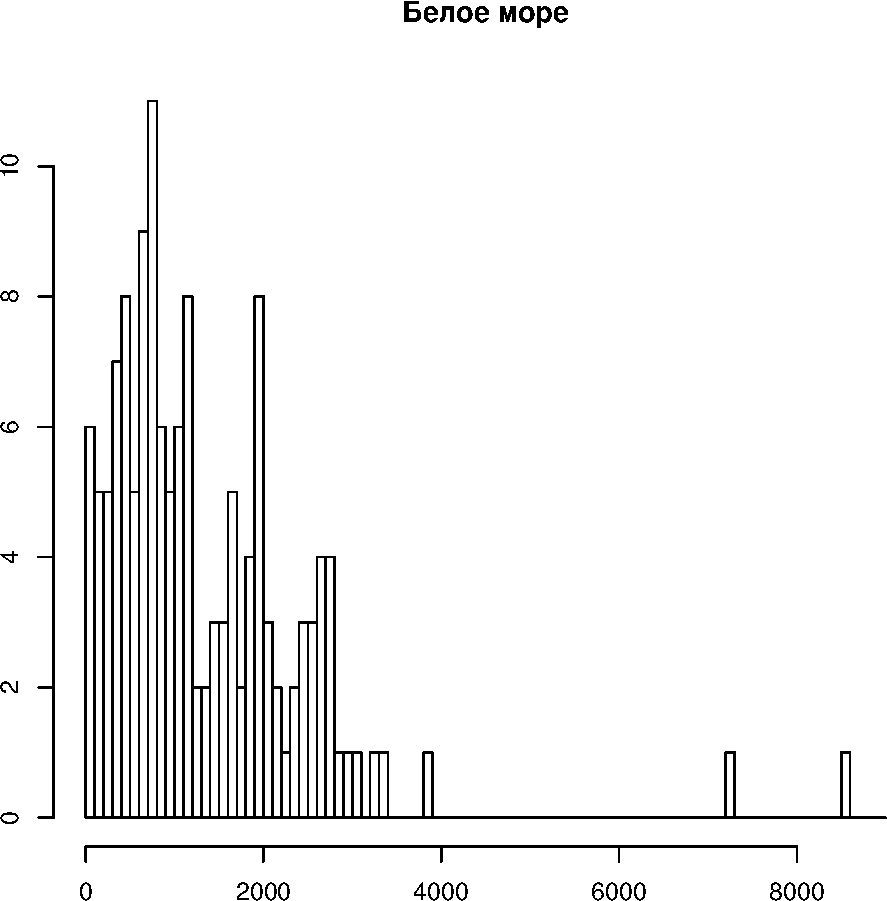
\includegraphics[height=.3\textheight]{../All_N/Nmean_hist_White.pdf}
		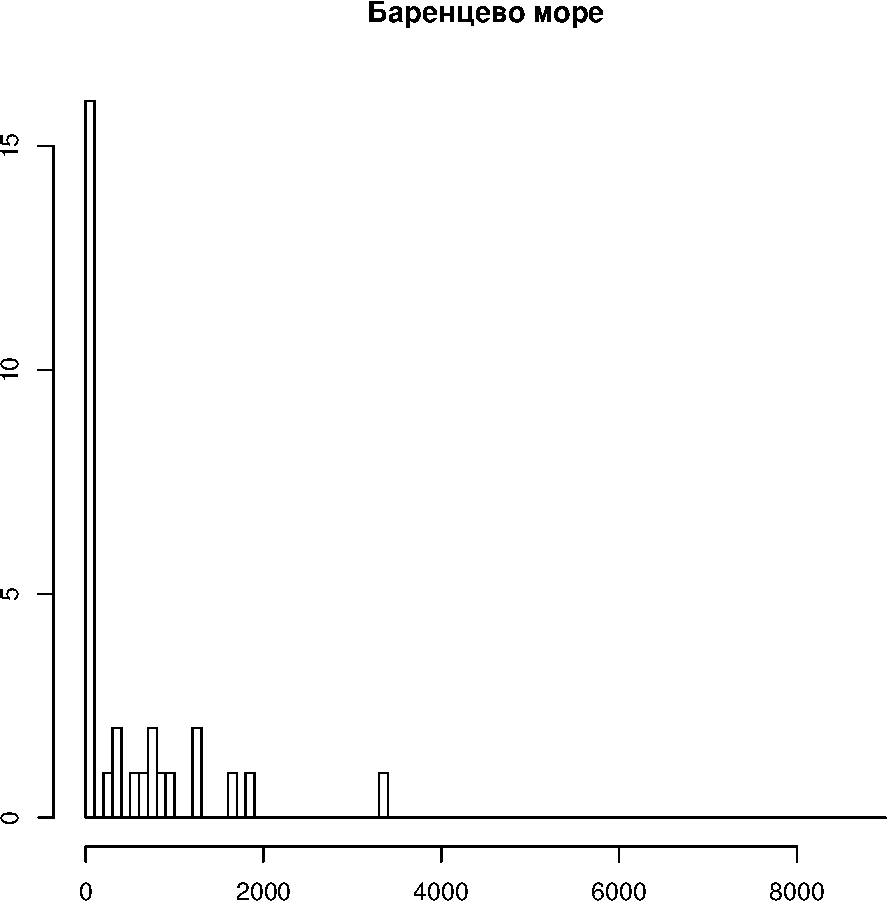
\includegraphics[height=.3\textheight]{../All_N/Nmean_hist_Barents.pdf}
	\caption{Частота встречаемости поселений с различным обилием {\it Macoma balthica}}
	{\footnotesize Примечание: по оси $X$ --- средняя численность {\it Macoma balthica}, экз./м$^2$ (шаг --- $100$~экз./м$^2$), по оси $Y$ 	--- частота встречаемости}
	\label{ris:Nmean_hist}
	\end{figure}
%
Наиболее часто встречаются поселения со средней численностью $700-800$~экз./м$^2$.
Отдельные районы Кандалакшского залива Белого моря не отличались по средней численности маком ($Kruskal-Wallis\ \chi^2 = 5,6$, $p = 0,2$). 
При сравнении средних обилий маком на разных участках в пределах одного горизонта не показало достоверных отличий (табл.~\ref{tab:Nmean_Kruskal_mareography_White}).
%
	\begin{table}[ht]
	\caption{Сравнение среднего обилия {\it M.~balthica} в пределах одного мареографического уровня в Белом море}
	\label{tab:Nmean_Kruskal_mareography_White}
	\begin{tabular}{|*{4}{p{0.2\textwidth}|}} \hline
	ма\-ре\-ографи\-ческий уровень & $Kruskal-Wallis\ \chi^2$ & $df$ & $p$ \\
	\hline
	СГЛ & $2,7$ & $5$ & $0,7$ \\
	\hline
	НГЛ & $5,8$ & $4$ & $0,2$ \\
	\hline
	ноль глубин & $0,16$ & $1$ & $0,7$ \\
	\hline
	ВСЛ & $1$ & $1$ & $0,3$ \\
	\hline
	\end{tabular}

	{\footnotesize Примечания: градации мареографического уровня: ВГЛ --- верхний горизонт литорали, СГЛ --- средний горизонт литорали, НГЛ --- нижний горидонт литорали, ВСЛ --- верхняя сублитораль}
	\end{table}
%
    Сравнение средних численностей на разных горизонтах в пределах одного участка показало различные результаты (табл.~\ref{tab:N2_area_mareography_Kruskal_White}). 
%
	\begin{table}[ht]
	\caption{Сравнение обилия {\it M.~balthica} в поселених на разном мареографическом уровне в Белом море}
	\label{tab:N2_area_mareography_Kruskal_White}
        \begin{tabular}{|p{0.25\textwidth}|*{4}{p{0.15\textwidth}|}} \hline
    участок & $Kruskal-Wallis\ \chi^2$ & $df$ & $p$ & \\
	\hline
    Клющиха & $19,7$ & $2$ & $5,2 \times 10^{-05}$ & ***\\
    \hline
    Клющиха (только литораль) & $1,1$ & $1$ & $0,31$ & \\
    \hline
    Сухая & $0,0057$ & $1$ & $0,94$ & \\
    \hline
    Лисья & $17,5$ & $2$ & $0,00016$ & ***\\
    \hline
    Лисья (только литораль) & $11,06$ & $1$ & $0,00088$ & ***\\
    \hline
    Подпахта  & $2,3$ & $1$ & $0,13$ & \\
    \hline
    Горелый & $10,2$ & $3$ & $0,01658$ & ** \\
    \hline
    материк, Лувеньга & $2,4$ & $3$ & $0,50$ &  \\
    \hline
	\end{tabular}
    {\footnotesize Примечание: достоверность различий *** --- $p<0,001$; ** --- $p<0,05$; * --- $p<0,1$.}
	\end{table}
%
Для участков в Сухой салме, проливе Подпахта, материковой литорали в Лувеньге варьирование численности между пробами перекрывало варьирование между горизонтами литорали.
При этом для участков в бухтах Клющиха и Лисья и на о.~Горелом Лувеньгских шхер  было показано достоверное влияние мареографического уровня на обилие маком. 
Интересно отметить, что в бухте Клющиха численность маком на нижнем и среднем горизонтах литорали не отличается ($403$~($7$)~экз./м$^2$), но в сублиторали она значительно выше ($1136$~($5$)~экз./м$^2$).
В бухте Лисья ситуация отличается, обилие маком на нижнем горизонте достоверно выше ($2832$~($10$)~экз./м$^2$), чем в среднем и в сублиторали ($1346$~($16$) и $1006$~($16$)~экз./м$^2$, соответсвенно). 



	\subsection{Баренцево море}

В Баренцевом море данные по обилию маком были получены для $12$ участков Мурманского побережья.
Минимальная средняя численность составляла $30$~экз./м$^2$ (г.~Дальнезеленецкая), что сравнимо с показателями для Белого моря. 
Максимальная средняя численность была значительно меньше, чем беломорская --- $3350$~экз./м$^2$ (Абрам-мыс) (табл.~\ref{tab:mean_N_Barents}). 
	\begin{footnotesize}
	\begin{longtable}{|p{2cm}|p{3cm}|p{1cm}|p{2cm}|p{1.5cm}|p{1cm}|*{3}{c|}}
	\caption{Средняя численность {\it Macoma balthica} на различных участках Баренцева моря}\label{tab:mean_N_Barents}\\
	\hline
	Район & Участок & год & ма\-ре\-ографи\-ческий уровень & число повторностей & площадь учета & $N$, экз./м$^2$ & $S_x$  & $D, \%$ 
	\\ \hline \endfirsthead
	\hline
	\multicolumn{9}{|c|}{продолжение таблицы \ref{tab:mean_N_Barents}} \\ \hline
	Район & Участок & год & ма\-ре\-ографи\-ческий уровень & число повторностей & площадь учета & $N$, экз./м$^2$ & $S_x$  & $D, \%$ 
	\\ \hline \endhead
	\hline 
	\multicolumn{9}{|c|}{продолжение таблицы \ref{tab:mean_N_Barents} на следующей странице}
	\\ \hline \endfoot
	\endlastfoot
	Западный Мурман & Ура-губа & 2005 & СГЛ & 3 & 1/30 & 1267 & 288,8 & 23
		\\ \cline{2-9}
		 & Печенга & 2005 & СГЛ & 3 & 1/30 & 767 & 218,6 & 29
		\\ \hline
	Кольский Залив & Северное Нагорное & 2005 & СГЛ & 2 & 1/30 & 390 & 90,0 & 23
		\\ \cline{2-9}
		 & Абрам-мыс & 2005 & СГЛ & 2 & 1/30 & 3350 & 520,0 & 16
		\\ \cline{3-9}
		 &  & 2008 & СГЛ & 5 & 1/20 & 540 & 208,5 & 39
		\\ \cline{4-9}
		 &  &  & НГЛ & 5 & 1/20 & 1804 & 78,6 & 4
		\\ \cline{2-9}
		 & Ретинское & 2005 & СГЛ & 2 & 1/30 & 660 & 300,0 & 45
		\\ \cline{2-9}
		 & Пала-губа & 2007 & СГЛ & 16 & 1/30 & 936 & 76,4 & 8
		\\ \cline{3-9}
		 &  & 2007 осень & НГЛ & 36 & 1/30 & 790 & 61,7 & 8
		\\ \cline{3-9}
		 &  & 2008 зима & НГЛ & 11 & 1/20 & 864 & 154,4 & 18
		\\ \cline{3-9}
		 &  & 2008 & НГЛ & 10 & 1/30 & 1644 & 192,5 & 12
		\\ \hline
	Восточный Мурман & Гаврилово & 2008 & СГЛ & 5 & 1/30 & 138 & 20,3 & 15
		\\ \cline{4-9}
		 &  & 2008 & НГЛ & 5 & 1/30 & 24 & 11,2 & 47
		\\ \cline{2-9}
		 & Ярнышная & 2007 & СГЛ & 36 & 1/30 & 70 & 9,6 & 14
		\\ \cline{3-9}
		 &  & 2008 & ВГЛ & 5 & 1/30 & 414 & 47,8 & 12
		\\ \cline{4-9}
		 &  & & НГЛ & 5 & 1/30 & 387 & 109,1 & 28
		\\ \cline{2-9}
		 & Дальнезеленецкая & 2002 & СГЛ & 43 & 1/30 & 52 & 7,0 & 13
		\\ \cline{3-9}
		 &  & 2003 & СГЛ & 48 & 1/30 & 34 & 6,6 & 20
		\\ \cline{3-9}
		 &  & 2004 & СГЛ & 44 & 1/30 & 32 & 5,3 & 16
		\\ \cline{3-9}
		 &  & 2005 & СГЛ & 30 & 1/30 & 30 & 4,5 & 15
		\\ \cline{3-9}
		 &  & 2006 & СГЛ & 28 & 1/30 & 39 & 6,0 & 16
		\\ \cline{3-9}
		 &  & 2007 & СГЛ & 33 & 1/30 & 72 & 6,6 & 9
		\\ \cline{3-9}
		 &  & 2008 & СГЛ & 72 & 1/30 & 72 & 5,5 & 8
		\\ \cline{4-9}
		 &  &  & ВГЛ & 10 & 1/30 & 30 & 8,9 & 30
		\\ \cline{4-9}
		 &  &  & НГЛ & 5 & 1/30 & 42 & 7,3 & 17
		\\ \cline{2-9}
		 & Шельпино & 2008 & СГЛ & 5 & 1/30 & 54 & 11,2 & 21
		\\ \cline{4-9}
		 &  &  & ВГЛ & 5 & 1/30 & 36 & 17,5 & 49
		\\ \cline{2-9}
		 & Порчниха & 2007 & СГЛ & 32 & 1/30 & 87 & 10,8 & 12
		\\ \cline{3-9}
		 &  & 2008 & СГЛ & 5 & 1/30 & 60 & 13,4 & 22
		\\ \cline{2-9}
		 & Ивановская & 2008 & ВСЛ & 5 & 1/20 & 1208 & 72,8 & 6
		\\ \hline
	\multicolumn{9}{p{16cm}}{Примечания: градации мареографического уровня: ВГЛ --- верхний горизонт литорали, СГЛ --- средний 	горизонт литорали, НГЛ --- нижний горидонт литорали, ВСЛ --- верхняя сублитораль. 

	$N$, экз./м$^2$ --- средняя численность {\it M.~balthica}. 
	$S_x$ --- ошибка среднего.
	 $D, \%$ ---  точность учета.
	
	В обозначении числа повторностей индекс ''и'' означает интегральную пробу, в этом случае в графе площадь учета указано сколько проб какой площади 	объединялись в одну.}
	\end{longtable}
	\end{footnotesize}
%
Среди иследованных, наиболее часто встречались поселения со средним обилием менее $100$~экз./м$^2$ (рис.~\ref{ris:N_region_Barents}).

Важно отметить, что для Мурманского побережья Баренцева моря показаны различия между отдельными районами: Западным, Восточным Мурманом и Кольским заливом (\ref{} \textcolor{red}{Гурьянова и ко?}). 
Это подтверждается нашими данными (рис.~\ref{ris:N_region_Barents}) по размаху варьирования среднего обилия в пределах районов ($Kruskal-Wallis\ \chi^2 = 17,6$, $p = 0,00015$).
%
	\begin{figure}[h]
		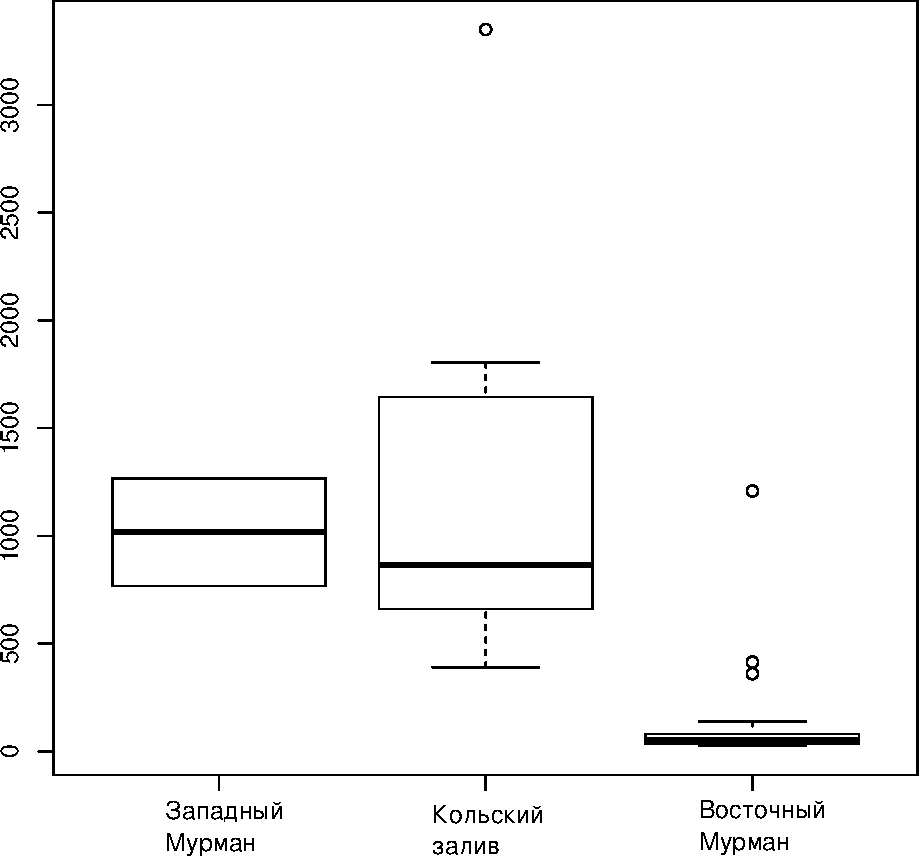
\includegraphics{../All_N/Nmean_region_Barents1.pdf}
	\caption{Варьирование среднего обилия {\it Macoma balthica} в разных районах Мурманского побережья Баренцева моря}
	{\footnotesize Примечание: По оси абсцисс --- численность {\it M.~balthica}, ~экз./м$^2$.

	На графике: жирная горизонтальная линия --- медиана, границы ''ящика'' --- 1 и 3 квартили, ''усы'' --- $1,5$ интерквартильного расстояния, точки - значения выпадающие за $1,5$ интерквартильных расстояния}
	\label{ris:N_region_Barents}
	\end{figure}
%
На литорали Восточного Мурмана численность {\it M.~balthica} в основном не превышала $100$~экз./м$^2$. 
Единственное исключение ---\ литораль губы Ярнышная, где численность маком достигала $410$~($12$)~экз./м$^2$. 
Между тем, на единственном участке, где были учеты в сублиторали, в губе Ивановской, численность на порядок выше, чем ее значения на литорали Восточного мурмана, и составляет $1200$~экз./м$^2$. 
В Кольском заливе минимальные значения обилия были отмечены на литорали в районе Северного Нагорного ($390$~($23$)~экз./м$^2$). 
Максимальных значений численности как для региона, так и для всей исследованной части Мурманского побережья, достигали поселения маком на учатске в районе Абрам-мысса ($3350$~($16$)~экз./м$^2$). 
На Западном Мурмане обилие флуктуировало вокруг $1000$~экз./м$^2$.  

При сравнении численности маком на различных мареографических уровнях различия между горизонтами литорали были показаны для губ Гаврилово и Ярнышная (табл.~\ref{tab:N2_area_mareography_Kruskal_Barents}).
В Гаврилово средняя численность {\it M.~balthica} в среднем горизонте литорали превышала аналогичные значения для нижнего горизонта на порядок ($138$~($15$) и $24$~($47$)~экз./м$^2$, соответственно).
В губе Ярнышная численность маком в верхнем и нижнем горизонтах не различалась ($414$~($12$) и $360$~($43$)~экз./м$^2$, соответсвенно), в то время как в среднем горизонте литорали она была значительно ниже ($70$~($14$)~экз./м$^2$).  
%
	\begin{table}[ht]
	\caption{Сравнение обилия {\it Macoma balthica} в поселених на разном мареографическом уровне в Баренцевом море}
	\label{tab:N2_area_mareography_Kruskal_Barents}
        \begin{tabular}{|p{0.25\textwidth}|*{4}{p{0.15\textwidth}|}} \hline
    участок & $Kruskal-Wallis\ \chi^2$ & $df$ & $p$ & \\
    \hline
    Абрам-мыс &  $1,5$ & $1$ & $0,224$ & \\
    \hline
    Пала-губа & $0,4$ & $1$ & $0,54$ & \\
    \hline
    Гаврилово & $6,9$ & $1$ & $0,0084$ & *** \\
    \hline
    Ярнышная & $19,4$ &  $2$ &  $6,09 \times 10^{-5}$ & *** \\
    \hline
    Дальнезеленецкая & $1,6$ & $2$ & $0,45$ & \\
    \hline
    Шельпино & $0,7$ & $1$ & $0,39$ & \\
    \hline
	\end{tabular}
    {\footnotesize Примечание: достоверность различий *** --- $p<0,001$; ** --- $p<0,05$; * --- $p<0,1$.}
	\end{table}
%

    \subsection{Влияние состава грунта на численность {\it Macoma balthica}}
Нет сомнений, что основной параметр, определяющий обилие маком ---\ это доступные пищевые   ресурсы.   
Косвенным   показателем   наличия   пищевых   ресурсов   служит гранулометрический состав грунта и общее содержание органических веществ. 
Поэтому по полученым для участков на Баренцевом море данным мы провели корреляционный анализ связи среднего обилия маком на участке с характеристиками  грунта.  
В   результате  оказалось,   что   соотношение   песчаных  фракций   различного   размера влияет   на   обилие  {\it M.~balthica}  (табл.~\ref{tab:grunt_N_correlation_Barents}).  
%
	\begin{table}[ht]
	\caption{Сравнение обилия {\it Macoma balthica} в поселених на разном мареографическом уровне в Баренцевом море}
    \label{tab:grunt_N_correlation_Barents}
     \begin{tabular}{|*{4}{p{0.15\textwidth}|}} \hline
    фракция & $R_s$ & $p-value$ & \\
    \hline
    $>10$~мм & $-0,2$ &  $0,36$ & \\
    \hline
    $10 - 5$~мм & $-0,01$ & $0,98$ & \\
    \hline
    $5 - 3$~мм & $0,07$ & $0,87$ & \\
    \hline
    $3 - 1$~мм & $0,12$ & $0,78$ & \\
    \hline
    $1 - 0,5$~мм & $-0,74$ & $0,04$ & ** \\
    \hline
    $0,5 - 0,25$~мм & $-0,67$  & $0,07$ & * \\
    \hline
    $0,25 - 0,1$~мм & $0,71$ & $0,04$ & ** \\
    \hline
    $<0,1$~мм & $0,6$ &  $0,12$ & \\
    \hline
    доля органических веществ & $0,36$ & $0,38$ & \\
    \hline
	\end{tabular}
    
    {\footnotesize Примечание: $R_s$ --- корреляция Спирмена. \\
    достоверность различий *** --- $p<0,001$; ** --- $p<0,05$; * --- $p<0,1$.}
	\end{table}
%
При   этом  наблюдается   достоверная   отрицательная корреляция численности маком с долей крупного  песка и положительная — с долей мелкого.


%% для компиляции в lualatex!!
\documentclass[12pt, a4paper]{article}
\usepackage[english,russian]{babel}
\usepackage[warn]{mathtext}
%\usepackage[T2A]{fontenc}
%\usepackage[utf8]{inputenc}

\usepackage{xecyr} % Продукт Вашего покорного слуги ;)

\setmainfont{DejaVu Serif}

\usepackage{color}
\usepackage{amssymb,amsmath}
\usepackage{graphicx}
\usepackage{multicol}

\textheight=24cm           % высота текста
\textwidth=16cm            % ширина текста
\oddsidemargin=0pt         % отступ от левого края
\topmargin=-1.5cm          % отступ от верхнего края
\parindent=24pt            % абзацный отступ
\parskip=0pt               % интервал между абзацами
\tolerance=2000            % терпимость к "жидким" строкам
\flushbottom               % выравнивание высоты страниц
%\def\baselinestretch{1.5} % печать с большим интервалом

%\title{}
%\author{\copyright~~С.А.~Назарова \thanks{e-mail:~sophia.nazarova@gmail.com}}
%\date{}

\begin{document}



%\maketitle

%Эстуарий Лувеньги
\begin{figure}[h]

\begin{multicols}{3}
\hfill
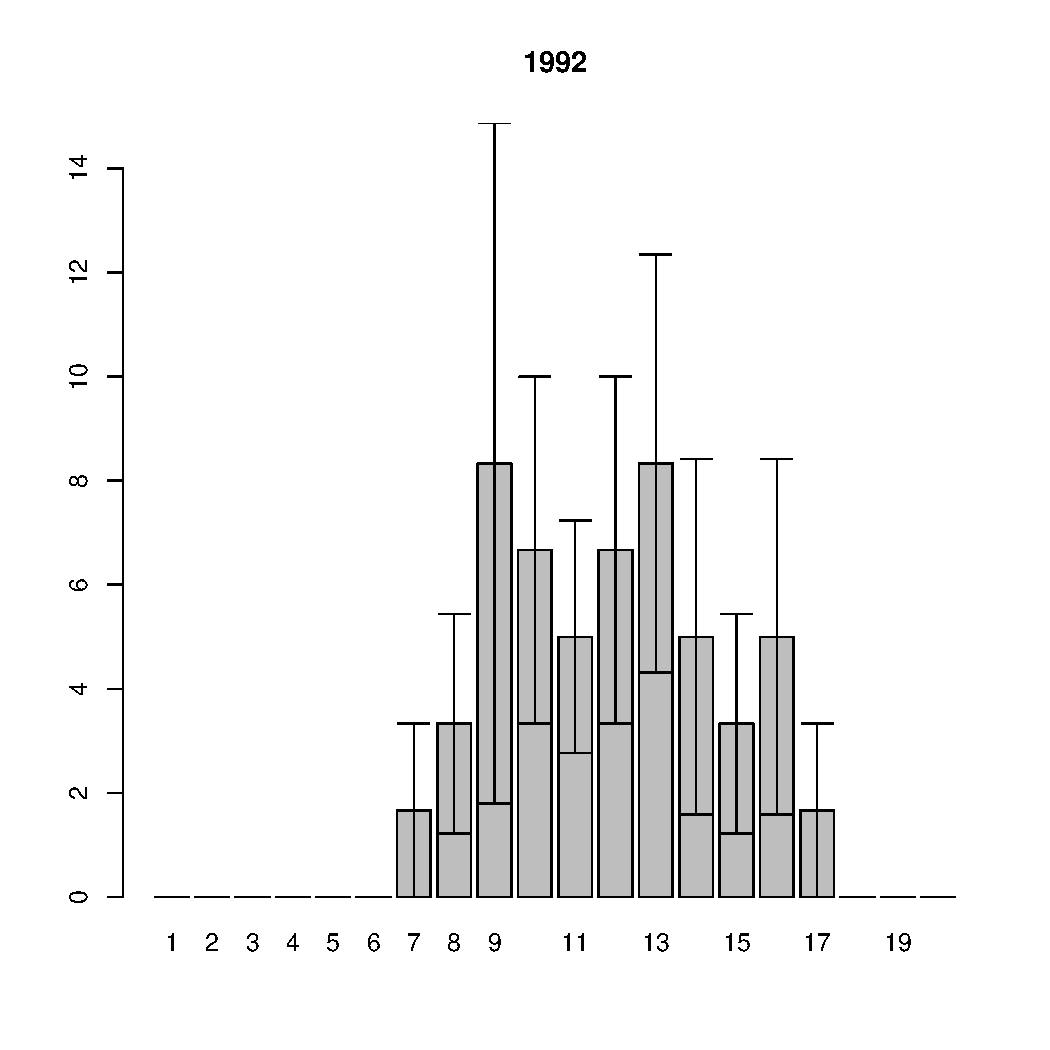
\includegraphics[width=60mm]{../White_Sea/Estuatiy_Luvenga/sizestr_1992_.pdf}
\hfill
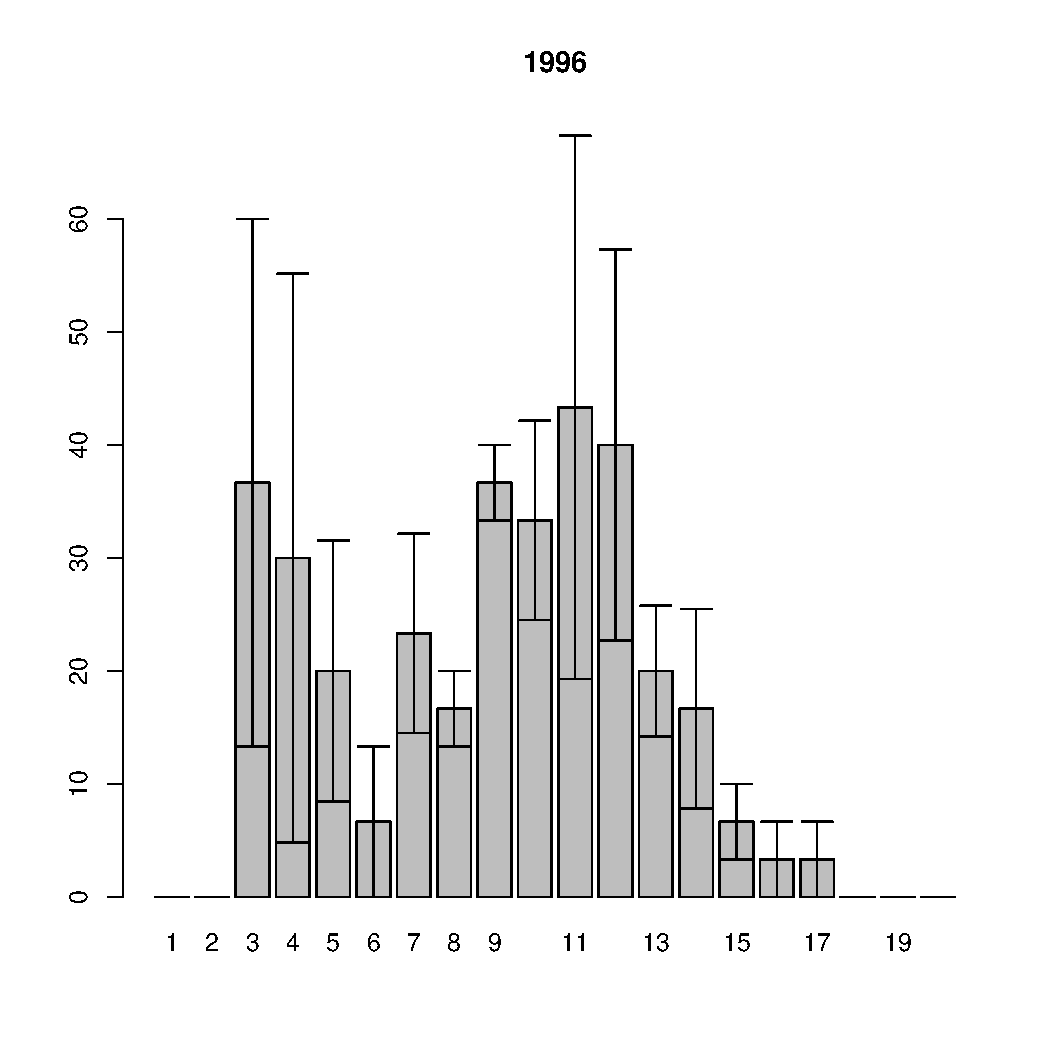
\includegraphics[width=60mm]{../White_Sea/Estuatiy_Luvenga/sizestr_1996_.pdf}
\hfill
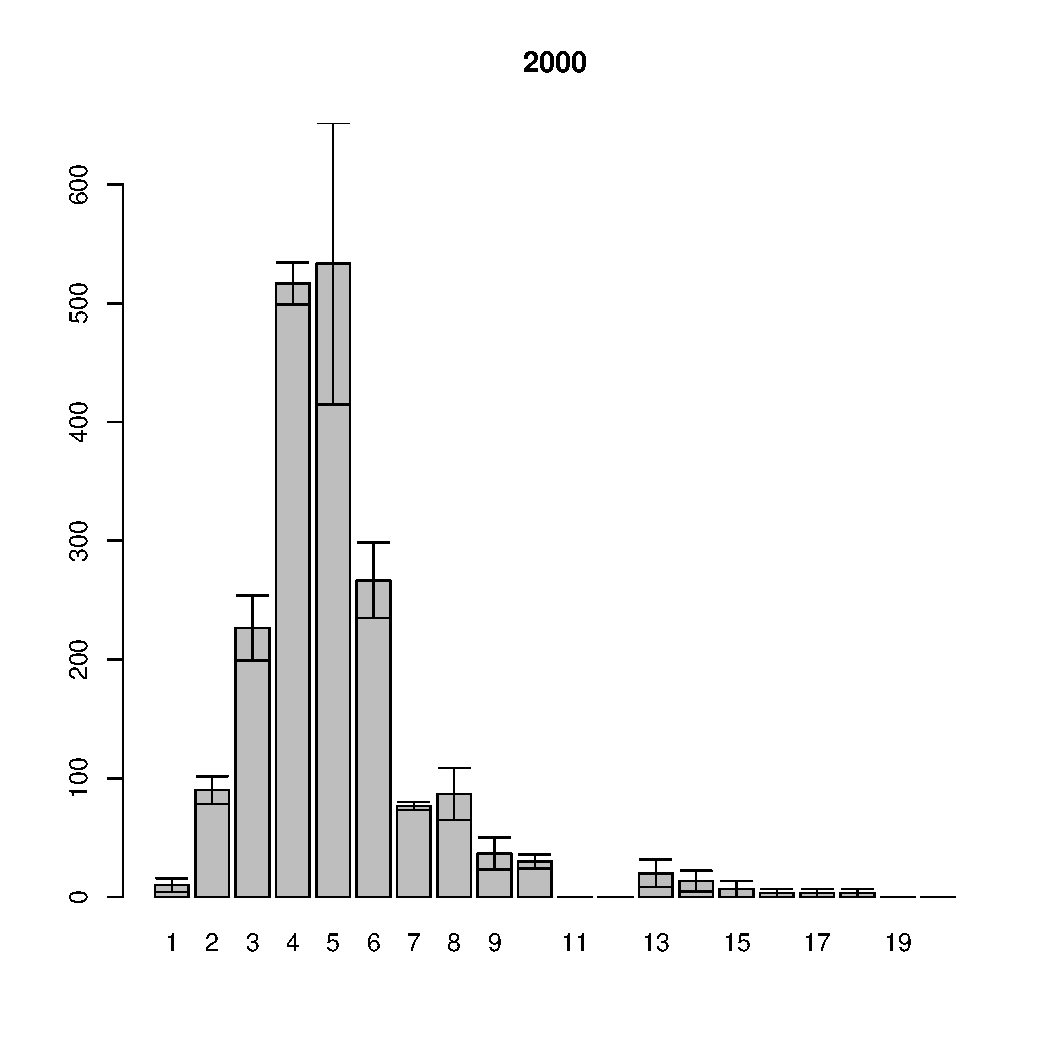
\includegraphics[width=60mm]{../White_Sea/Estuatiy_Luvenga/sizestr_2000_.pdf}
\end{multicols}

%\smallskip


\begin{multicols}{3}
\hfill
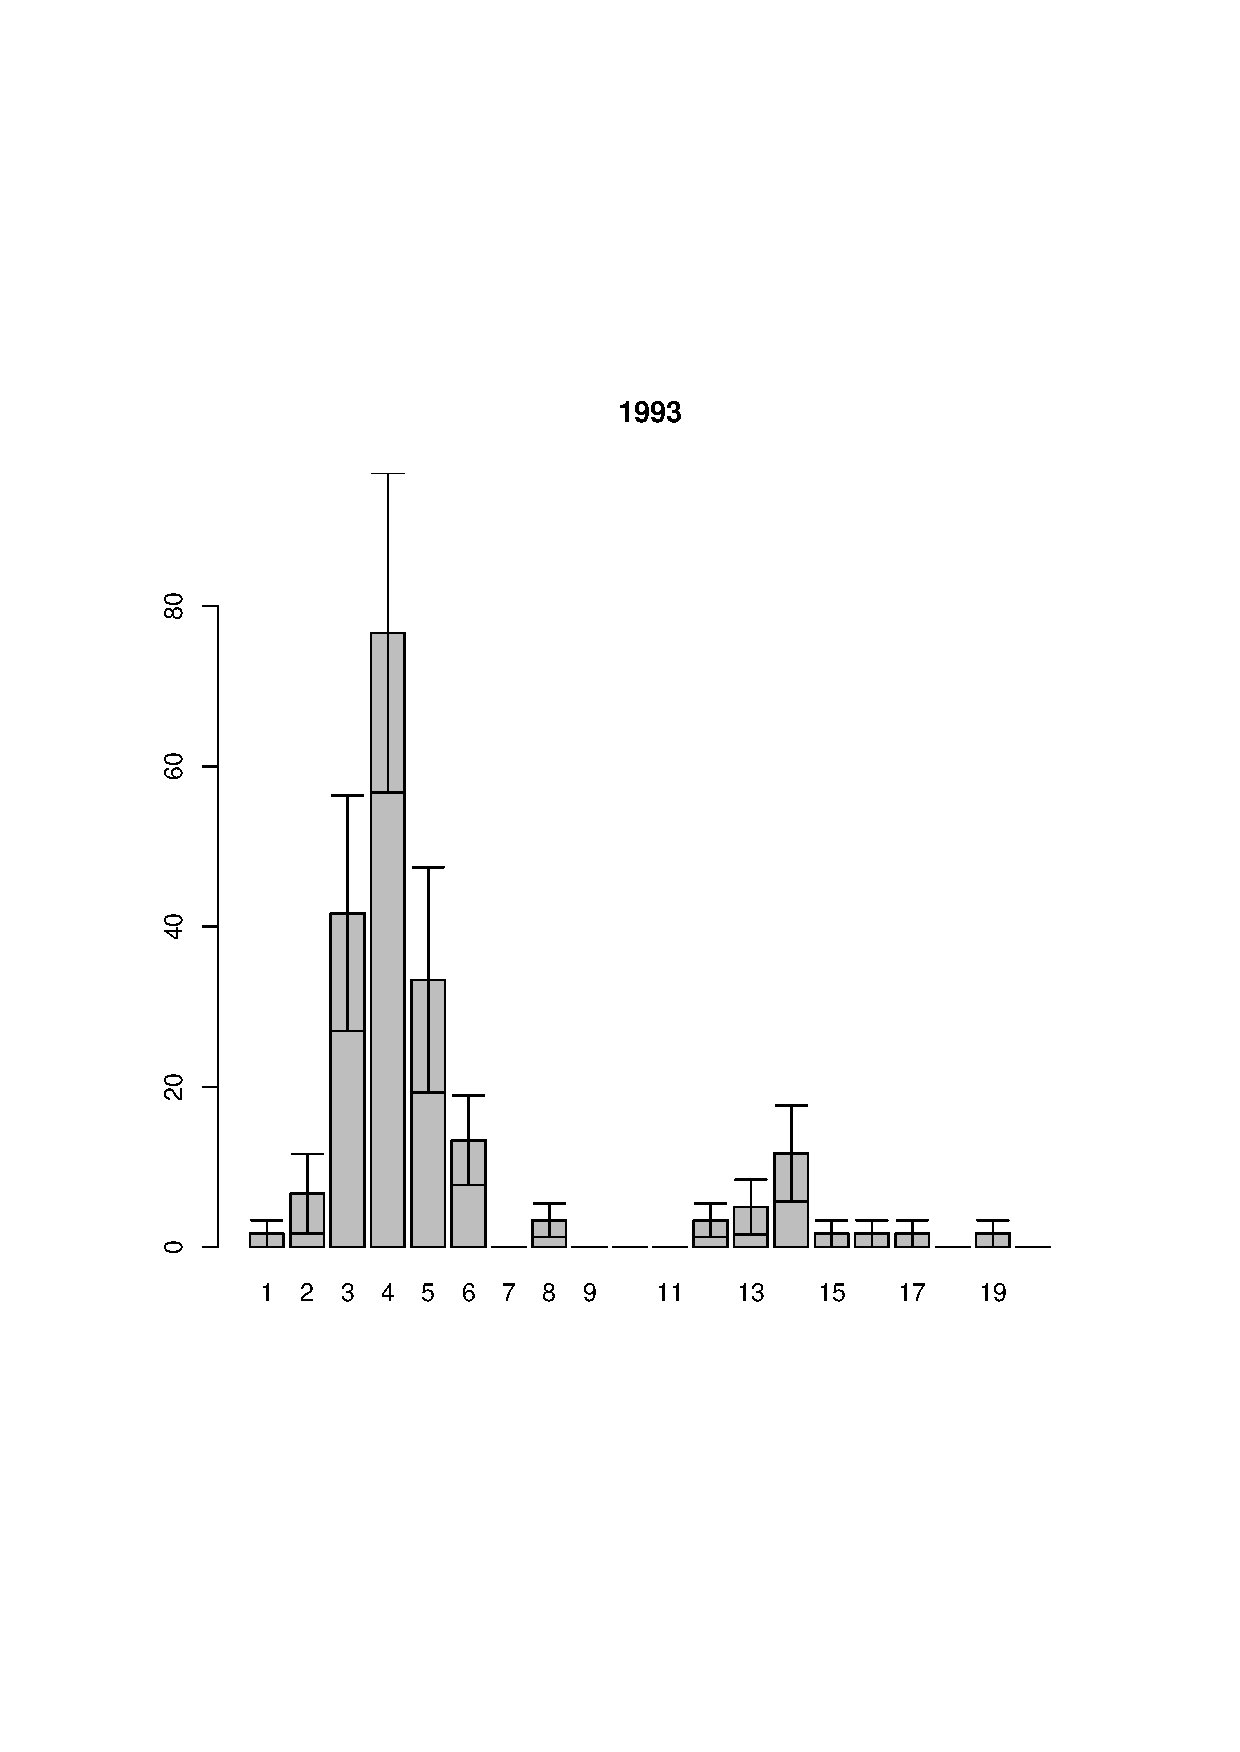
\includegraphics[width=60mm]{../White_Sea/Estuatiy_Luvenga/sizestr_1993_.pdf}
\hfill
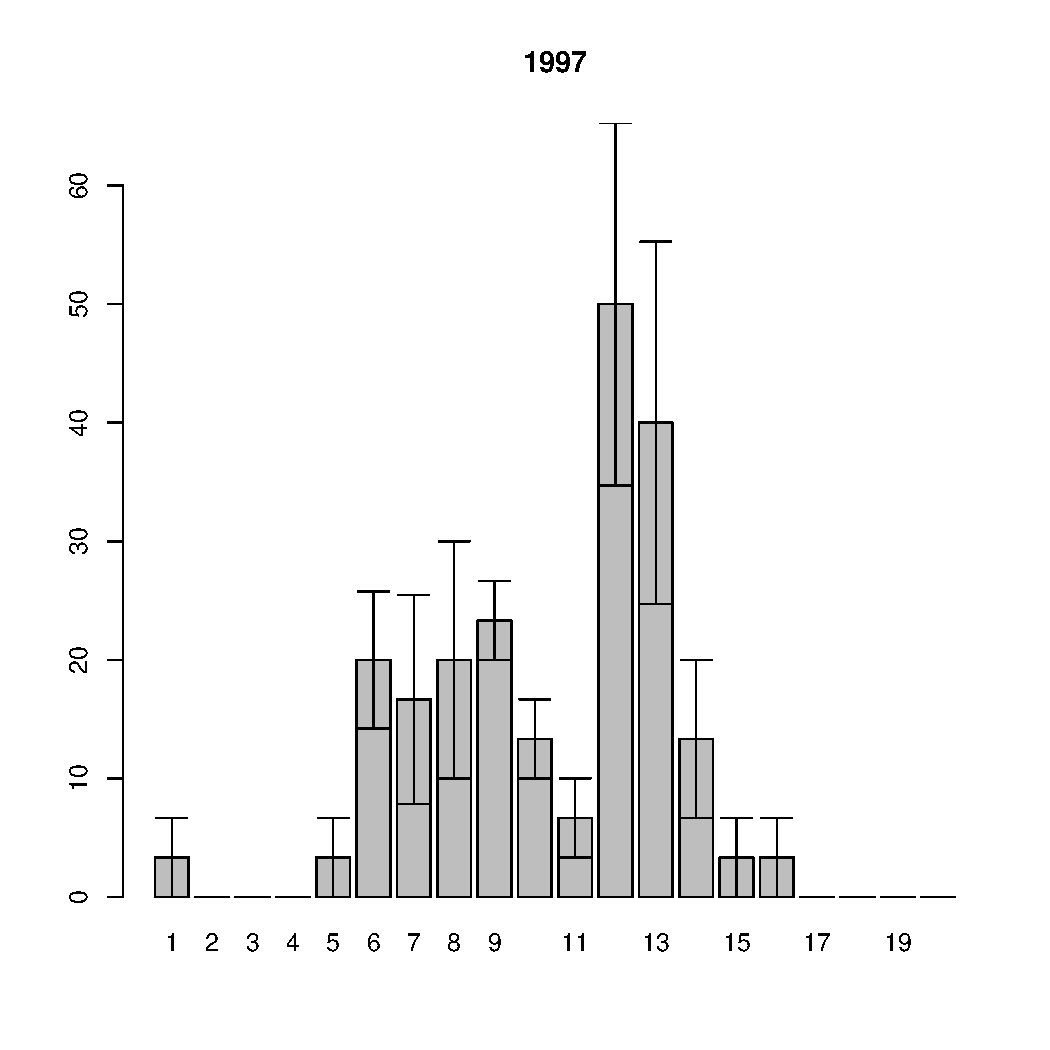
\includegraphics[width=60mm]{../White_Sea/Estuatiy_Luvenga/sizestr_1997_.pdf}
\hfill
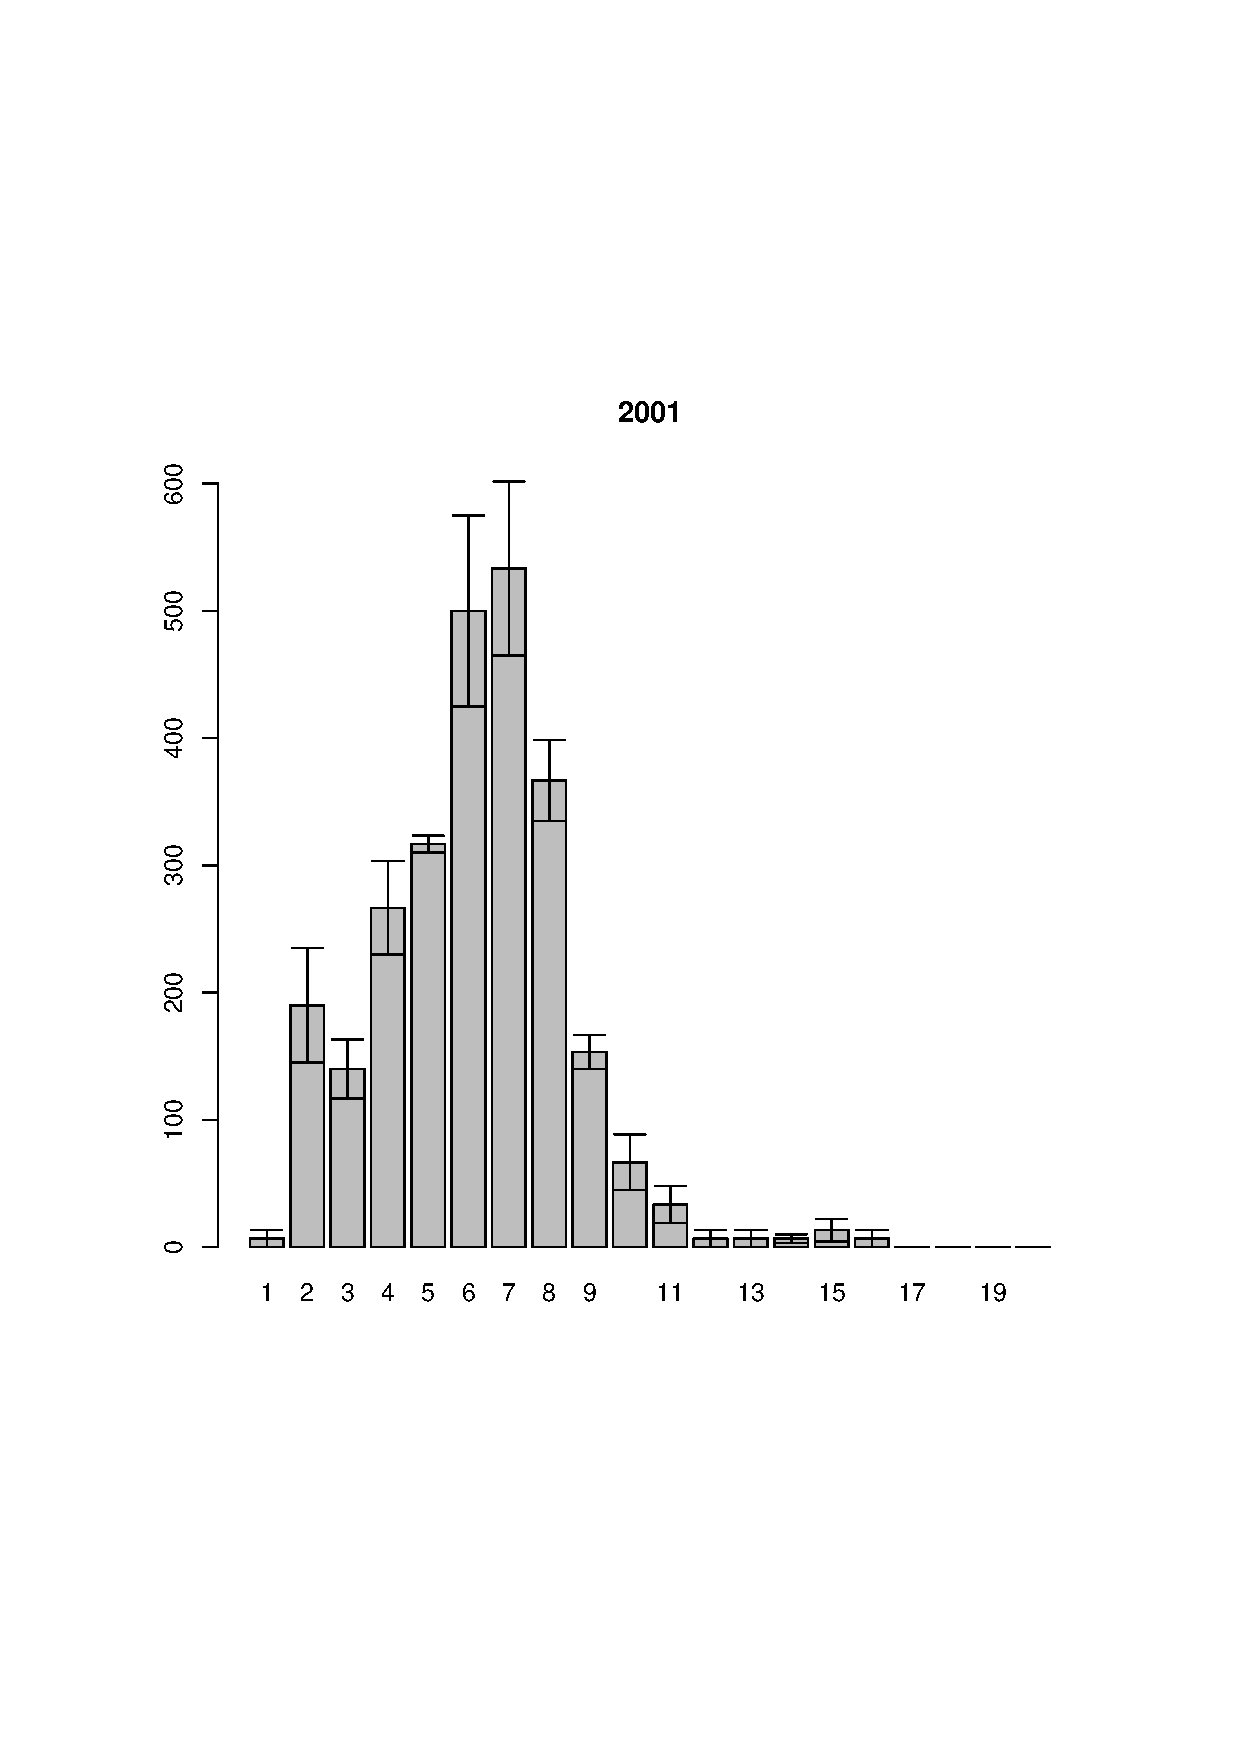
\includegraphics[width=60mm]{../White_Sea/Estuatiy_Luvenga/sizestr_2001_.pdf}
\end{multicols}

%\smallskip

\begin{multicols}{3}
\hfill
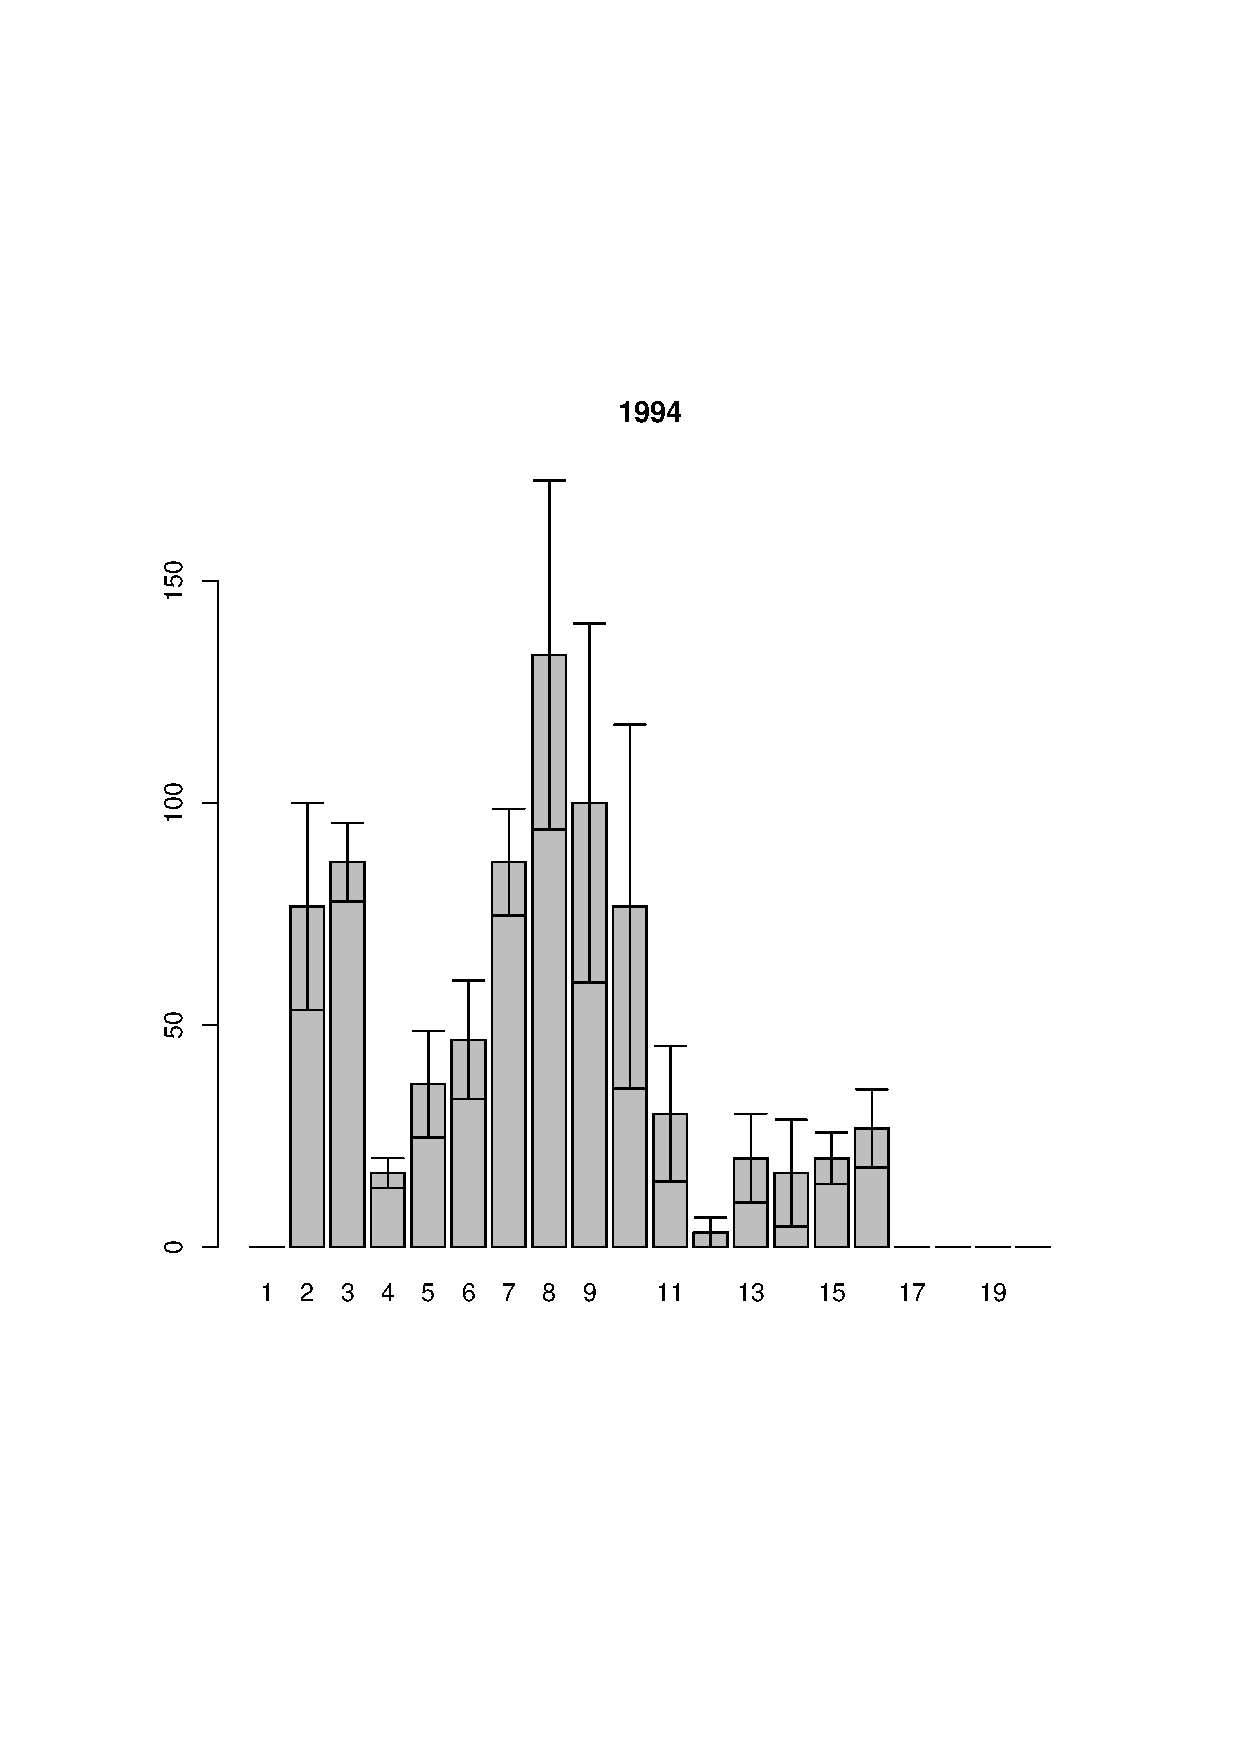
\includegraphics[width=60mm]{../White_Sea/Estuatiy_Luvenga/sizestr_1994_.pdf}
\hfill
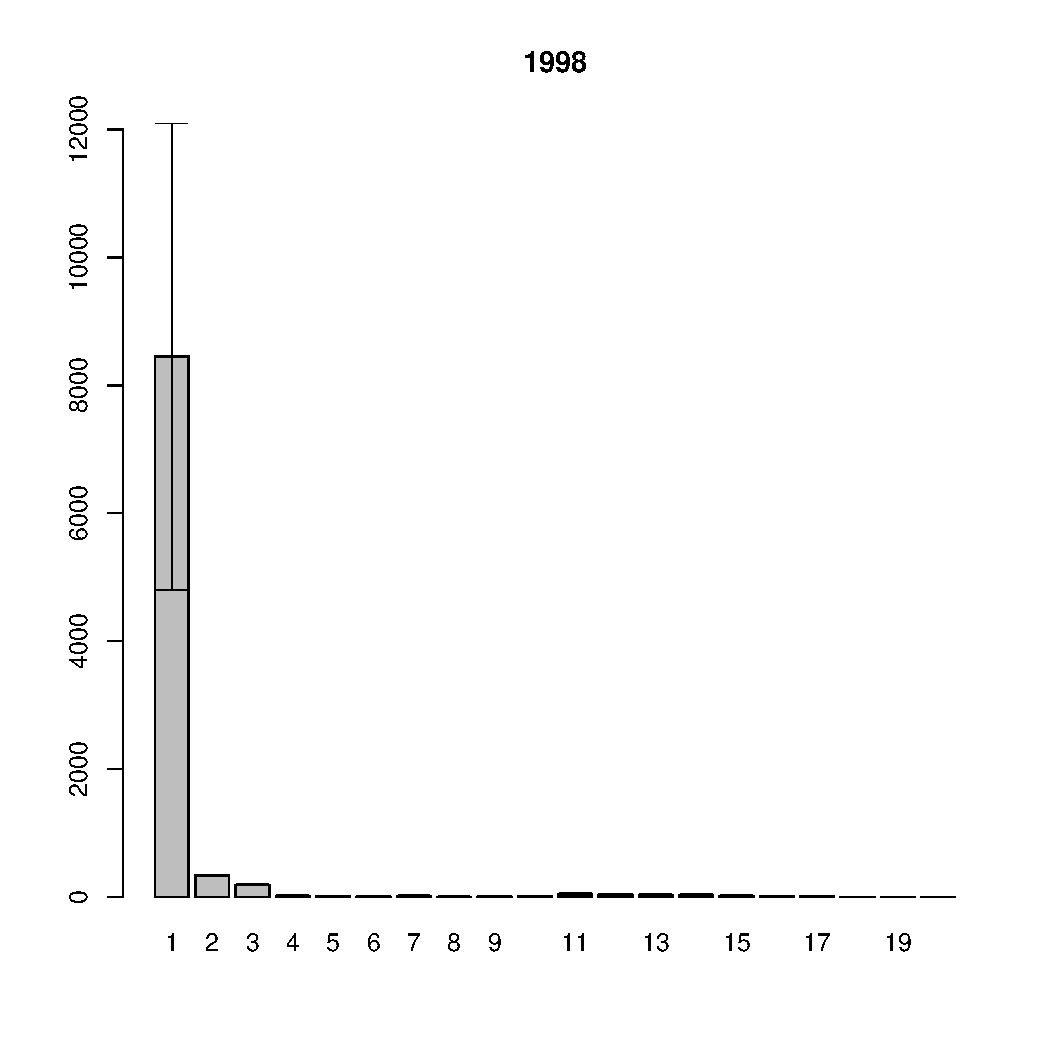
\includegraphics[width=60mm]{../White_Sea/Estuatiy_Luvenga/sizestr_1998_.pdf}
\hfill
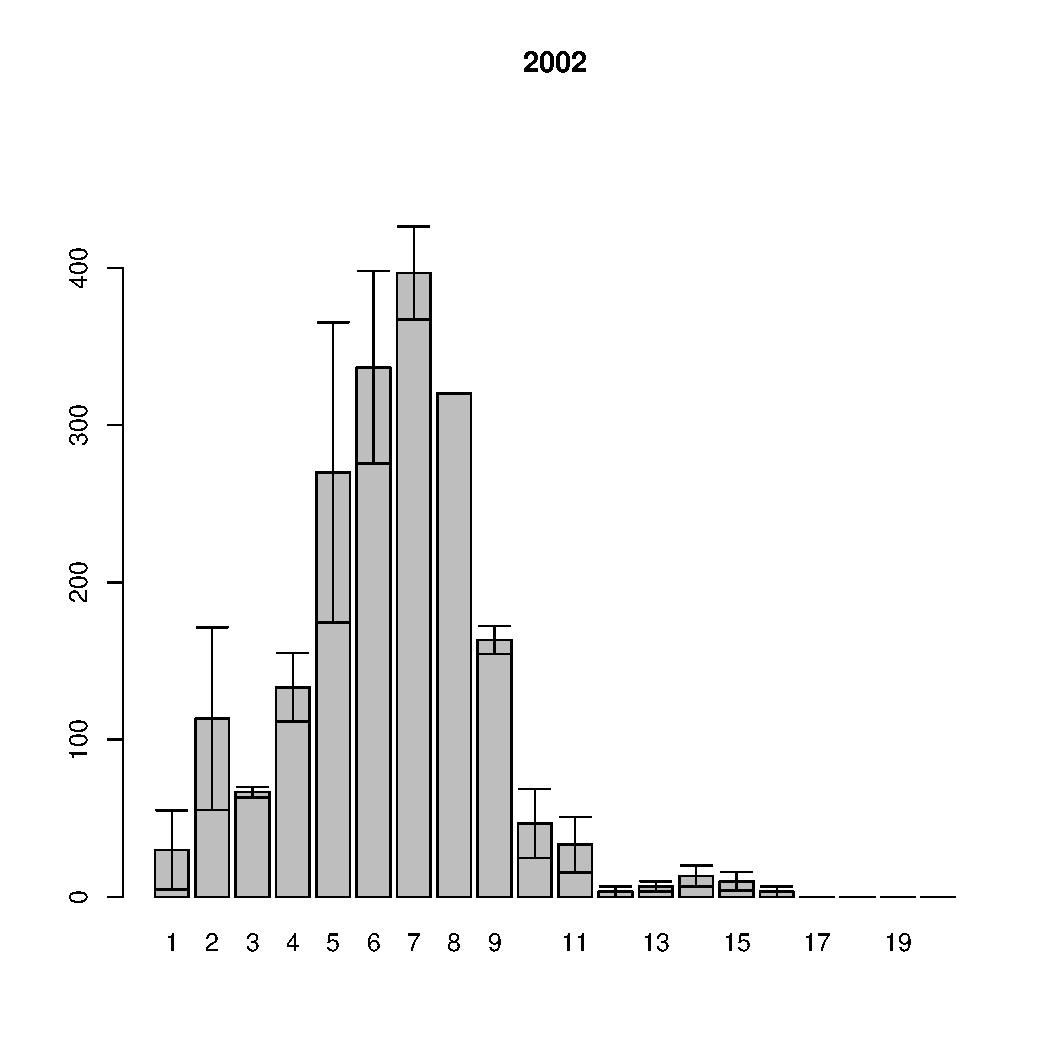
\includegraphics[width=60mm]{../White_Sea/Estuatiy_Luvenga/sizestr_2002_.pdf}
\end{multicols}

%\smallskip

\begin{multicols}{3}
\hfill
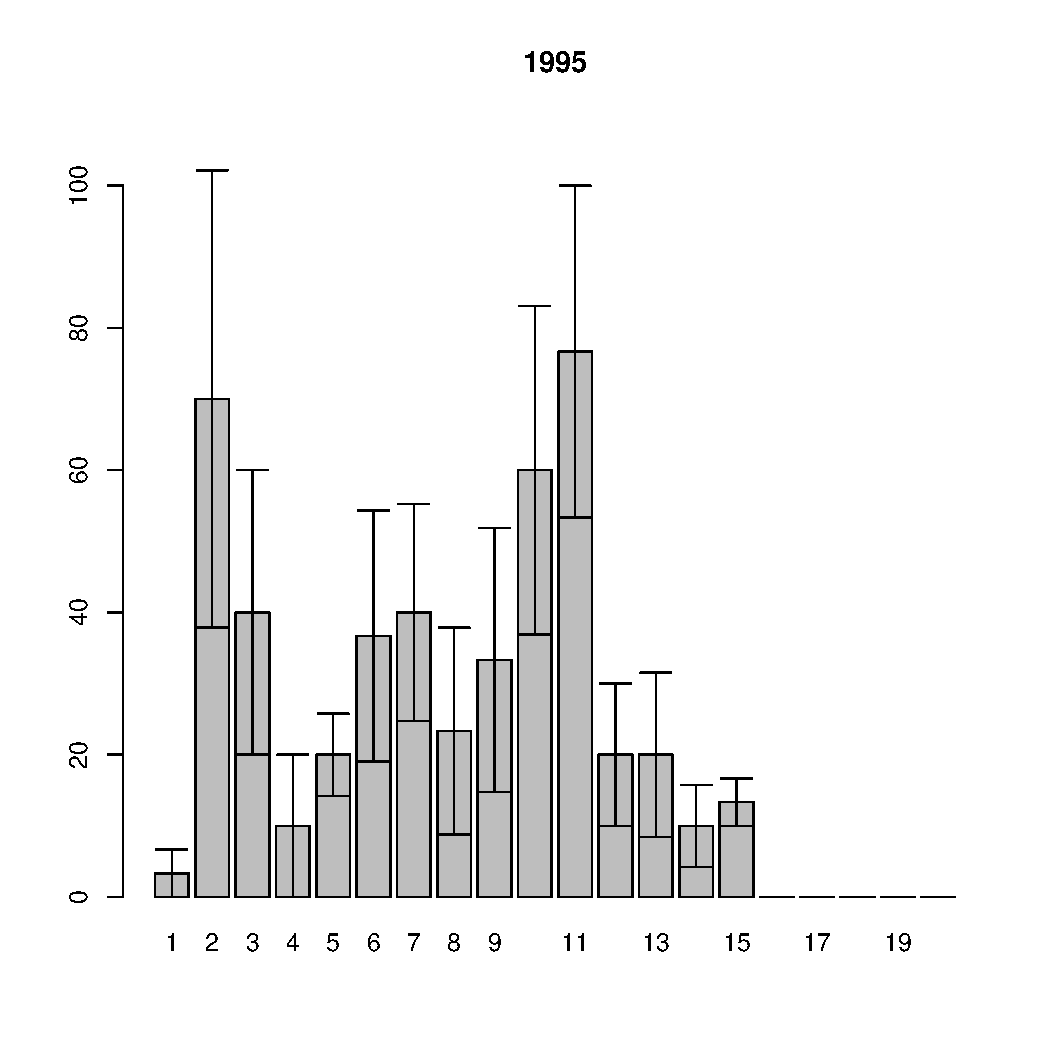
\includegraphics[width=60mm]{../White_Sea/Estuatiy_Luvenga/sizestr_1995_.pdf}
\hfill
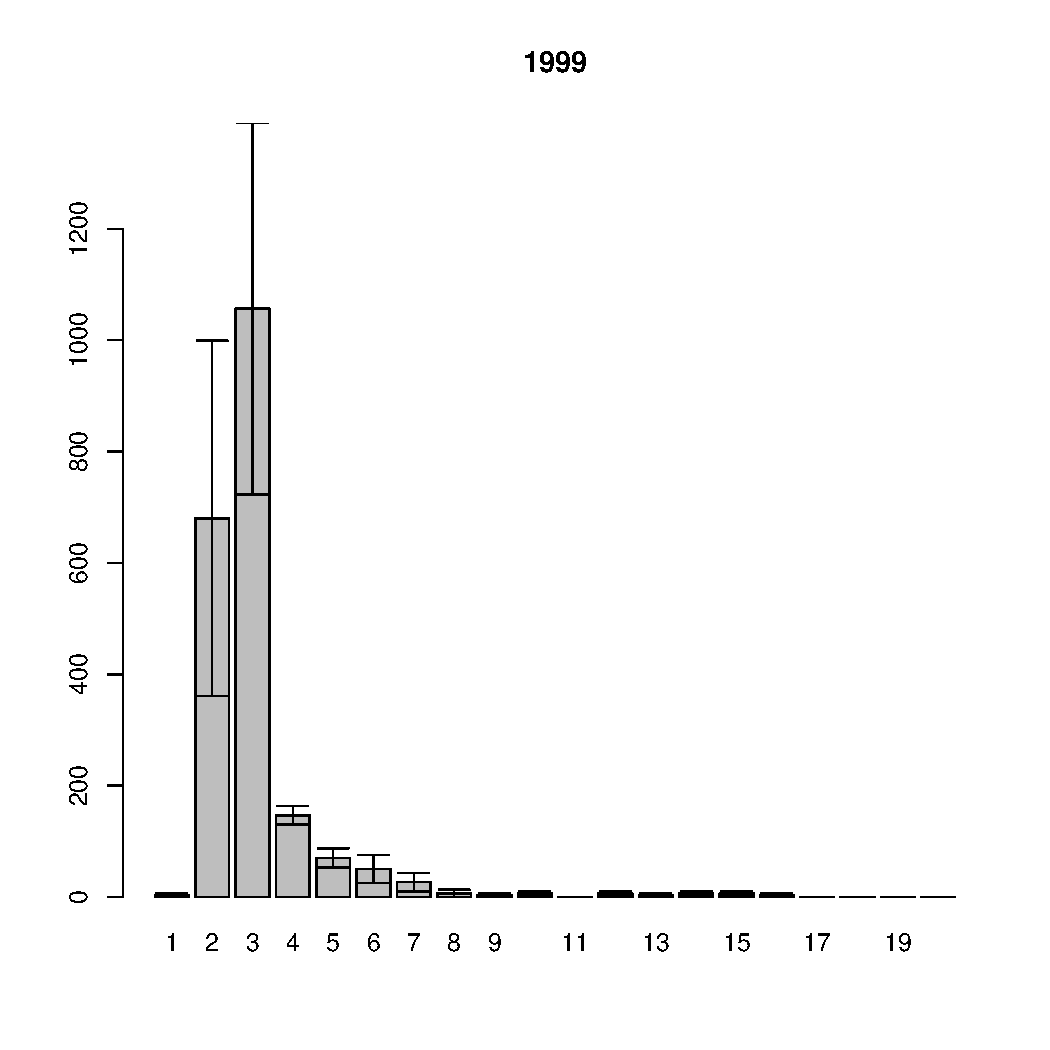
\includegraphics[width=60mm]{../White_Sea/Estuatiy_Luvenga/sizestr_1999_.pdf}
\hfill
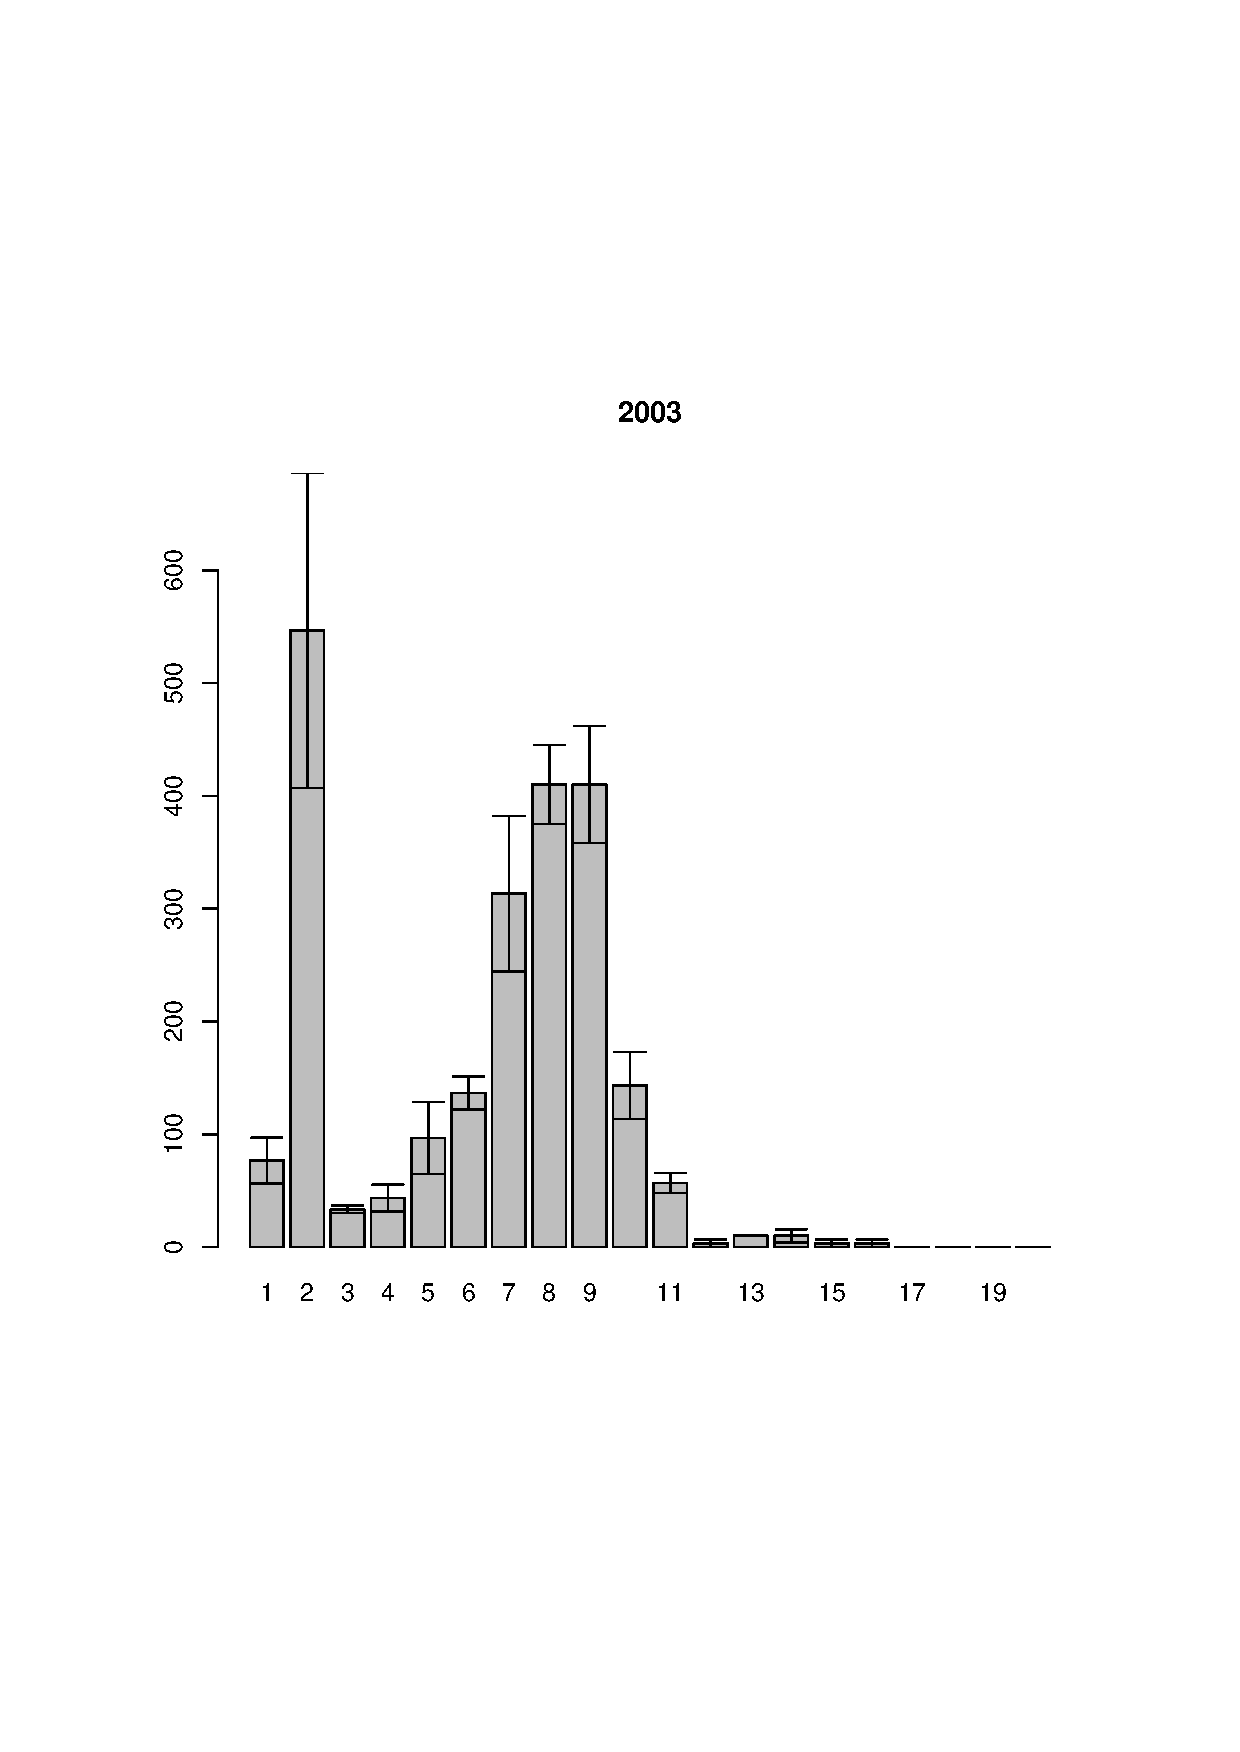
\includegraphics[width=60mm]{../White_Sea/Estuatiy_Luvenga/sizestr_2003_.pdf}
\end{multicols}


\caption{Размерная структура {\it Macoma balthica} в СГЛ эстуария р. Лувеньги}
\label{ris:size_str_estuary_Luv}
\end{figure}


\begin{figure}[h]

\begin{multicols}{3}
\hfill
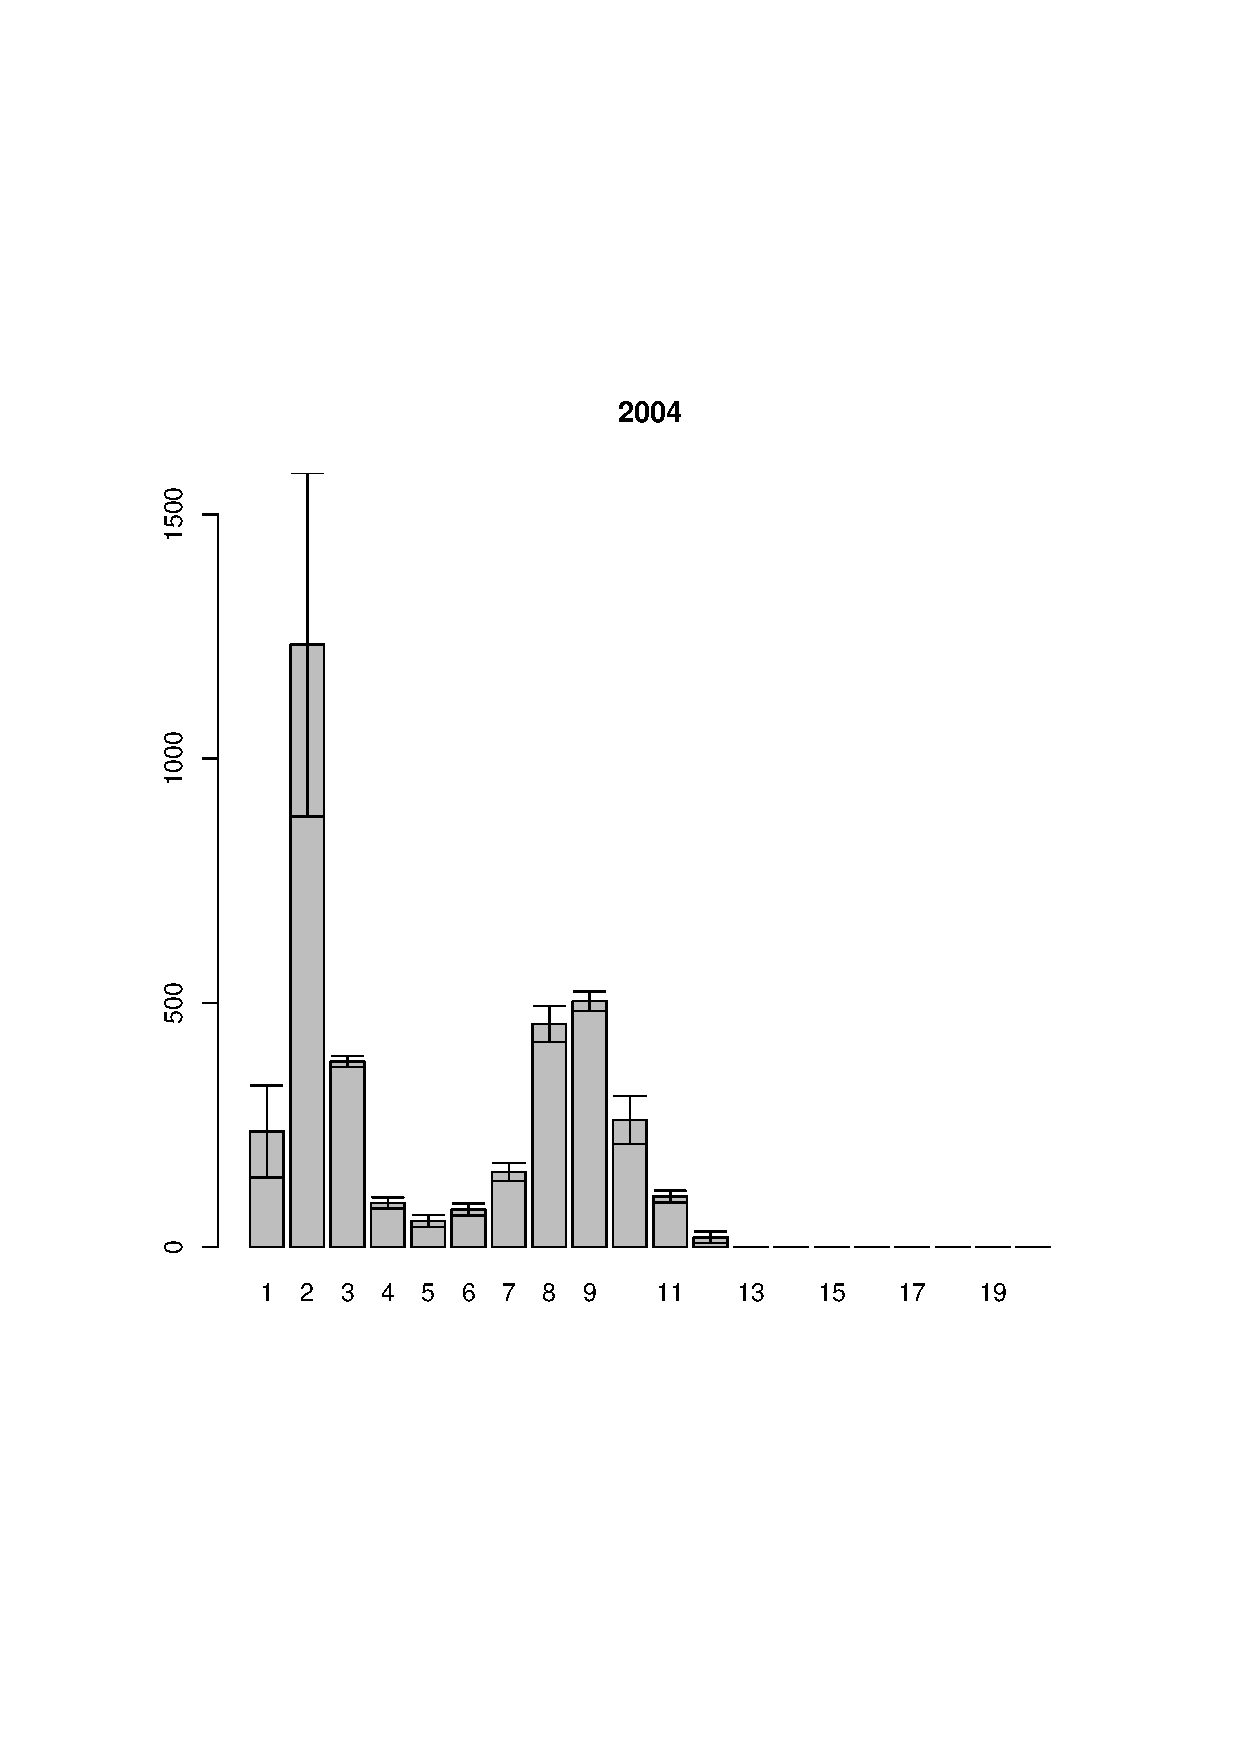
\includegraphics[width=60mm]{../White_Sea/Estuatiy_Luvenga/sizestr_2004_.pdf}
\hfill
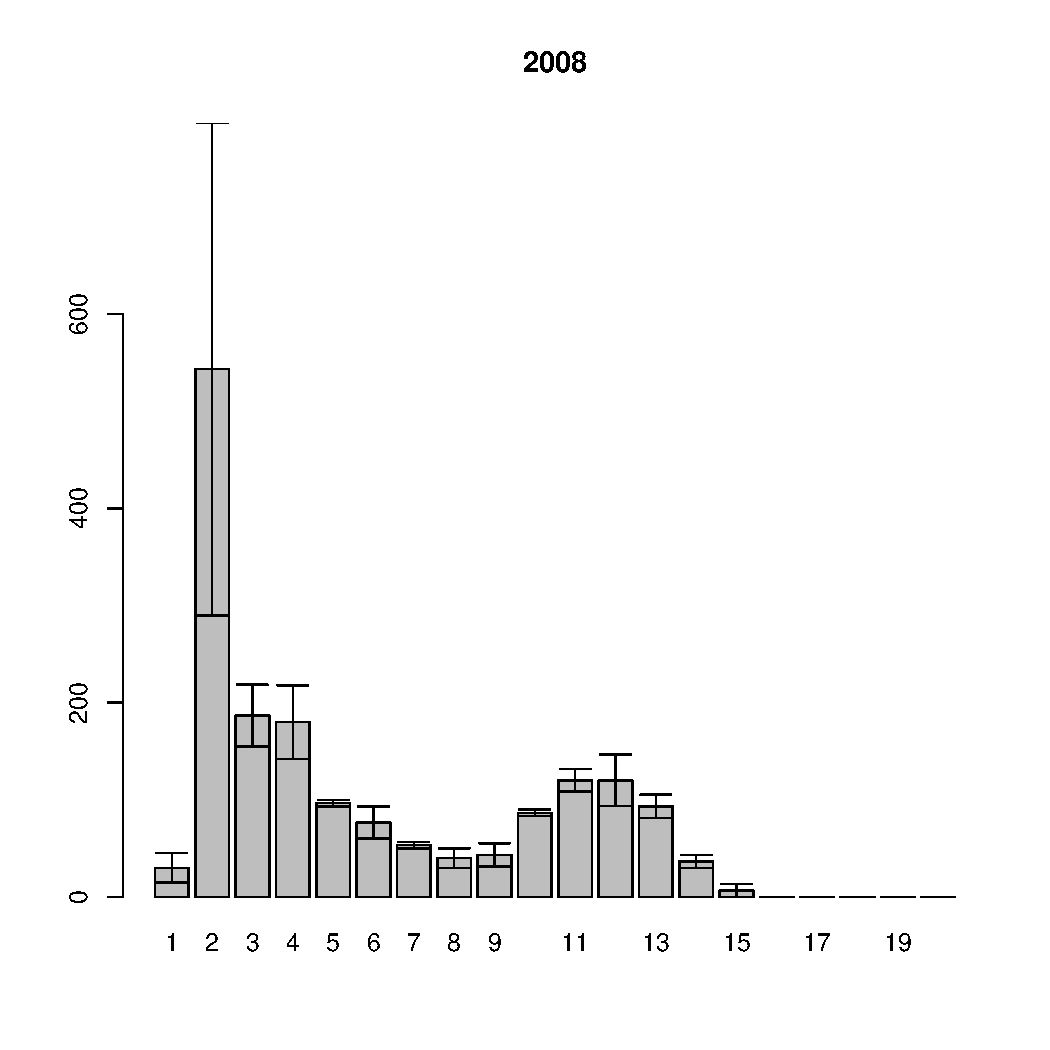
\includegraphics[width=60mm]{../White_Sea/Estuatiy_Luvenga/sizestr_2008_.pdf}
\hfill
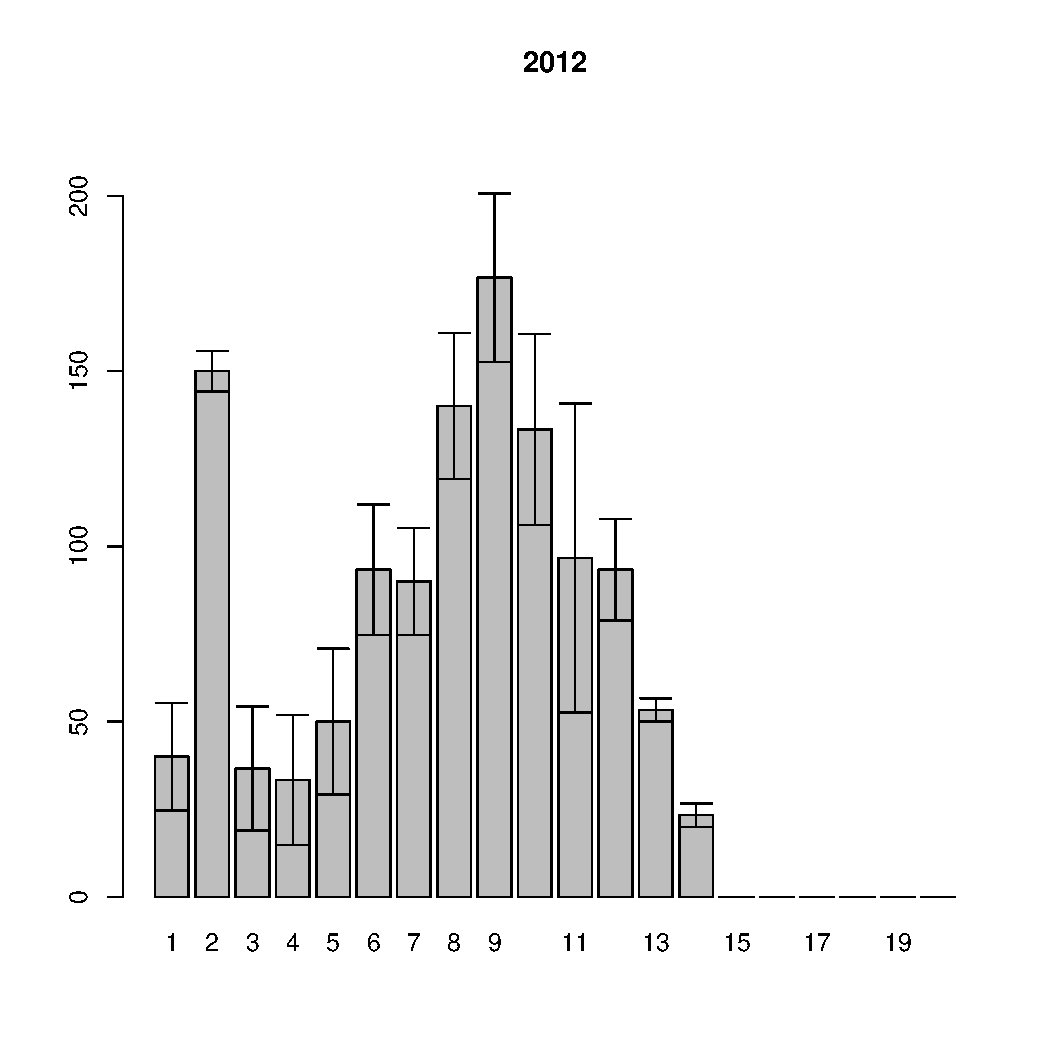
\includegraphics[width=60mm]{../White_Sea/Estuatiy_Luvenga/sizestr_2012_.pdf}
\end{multicols}

%\smallskip


\begin{multicols}{3}
\hfill
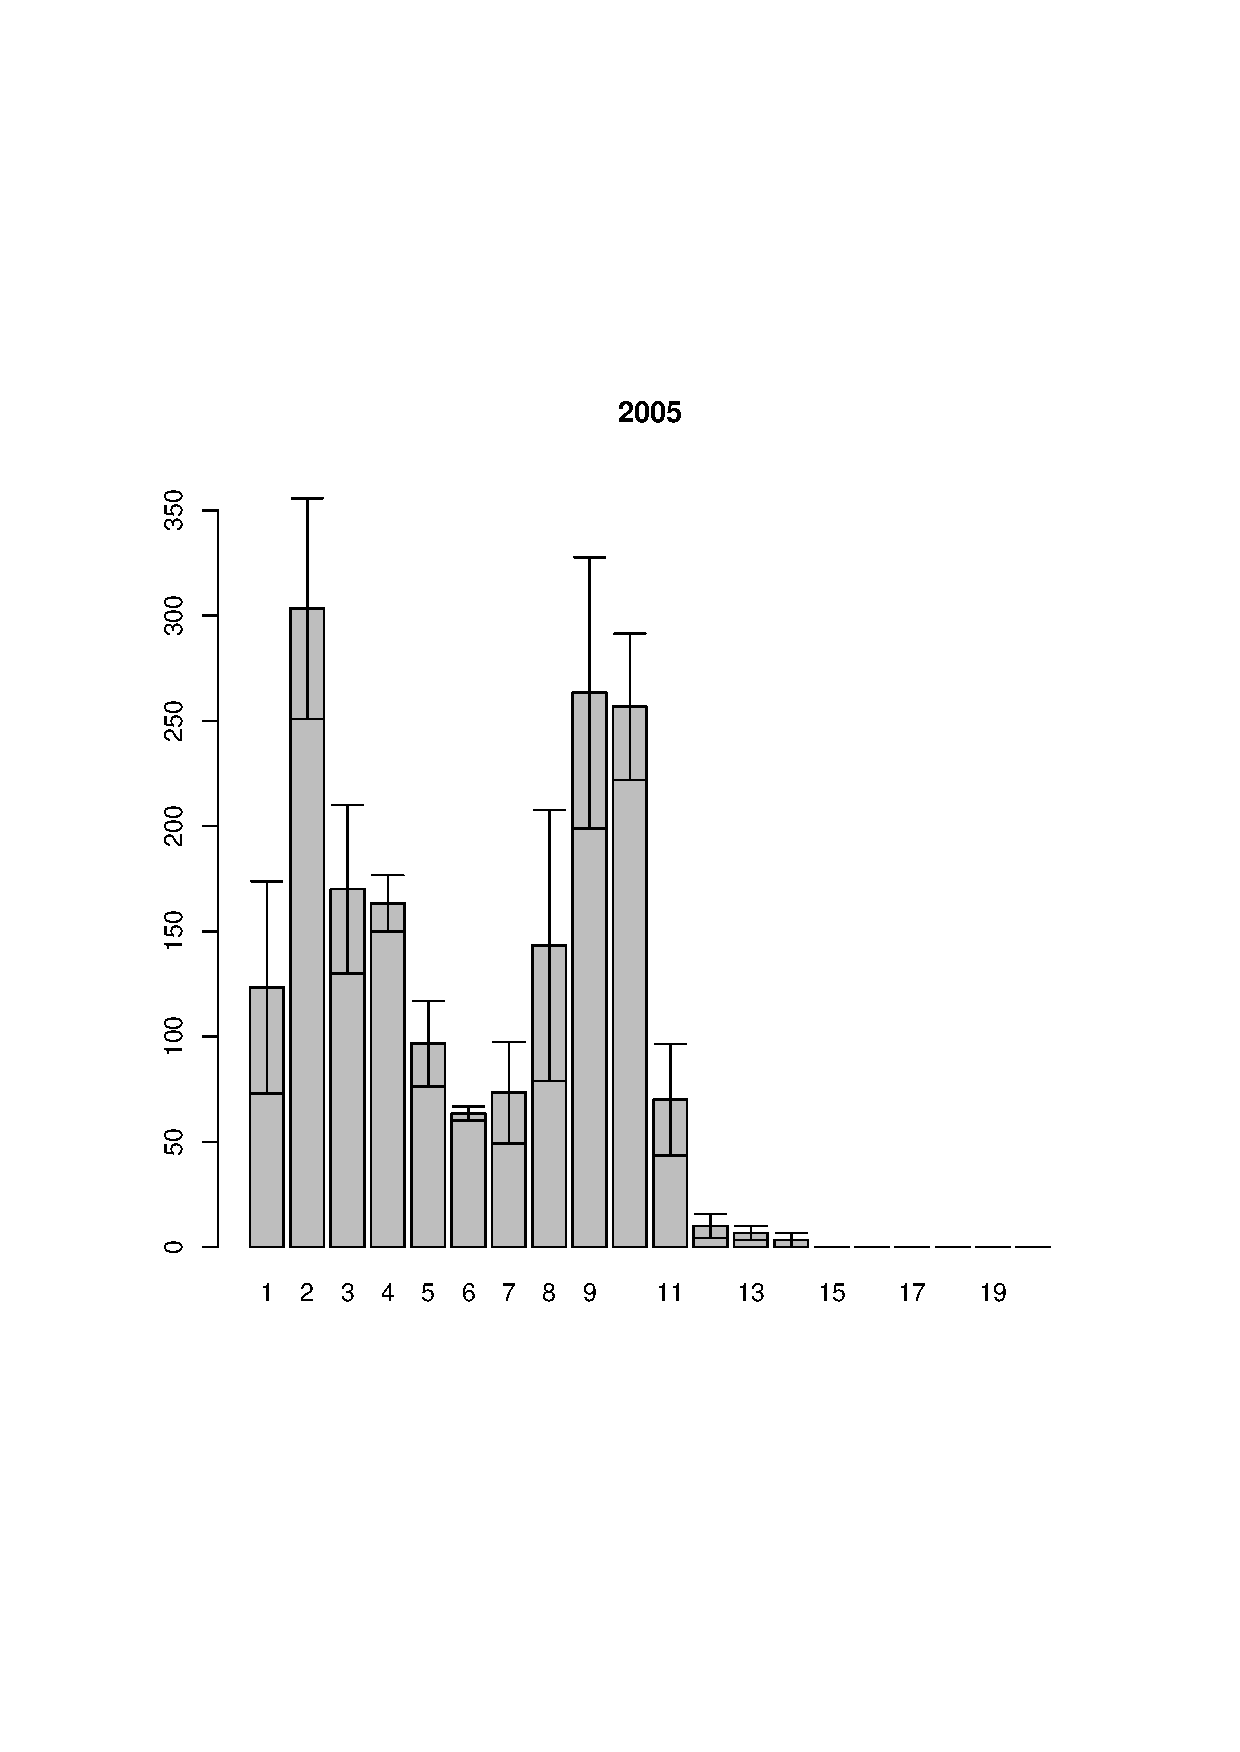
\includegraphics[width=60mm]{../White_Sea/Estuatiy_Luvenga/sizestr_2005_.pdf}
\hfill
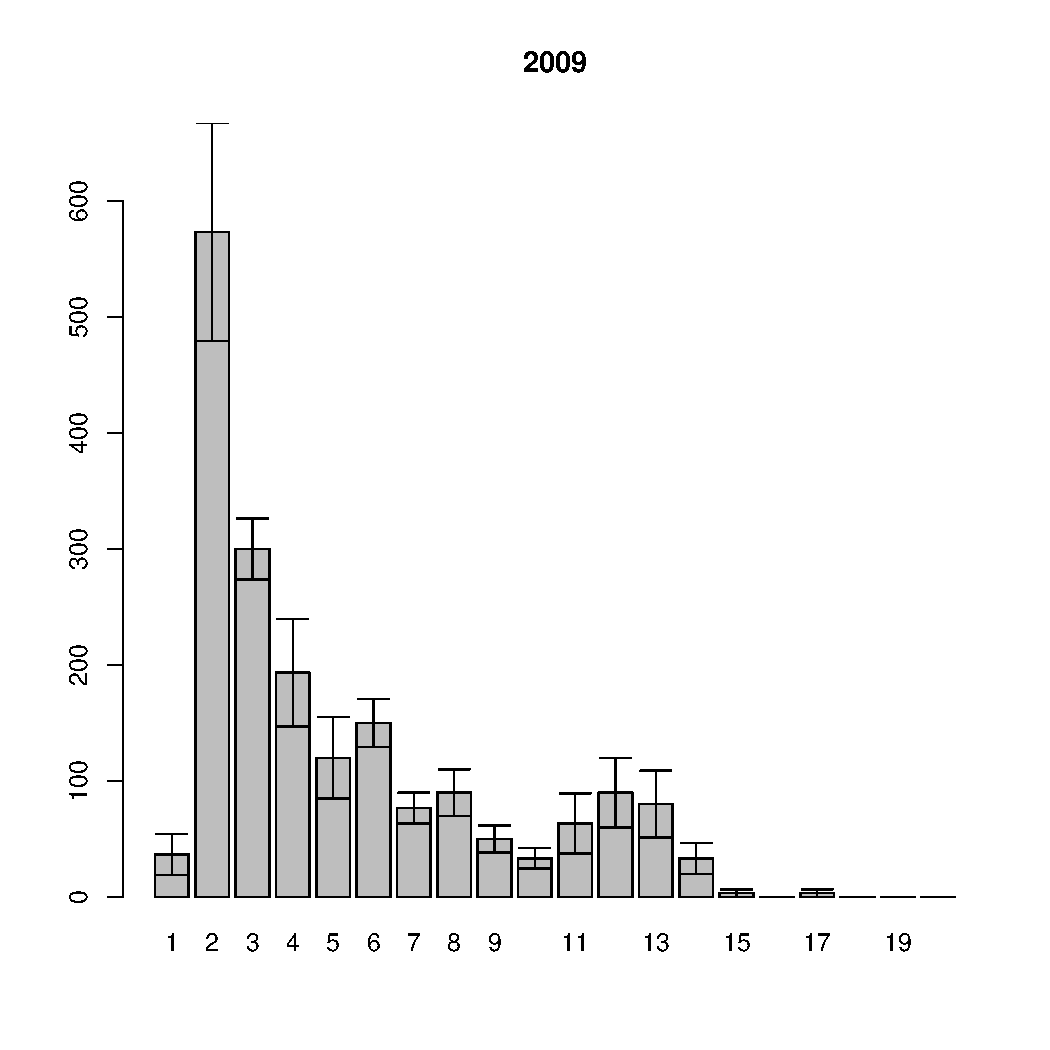
\includegraphics[width=60mm]{../White_Sea/Estuatiy_Luvenga/sizestr_2009_.pdf}
%\hfill
%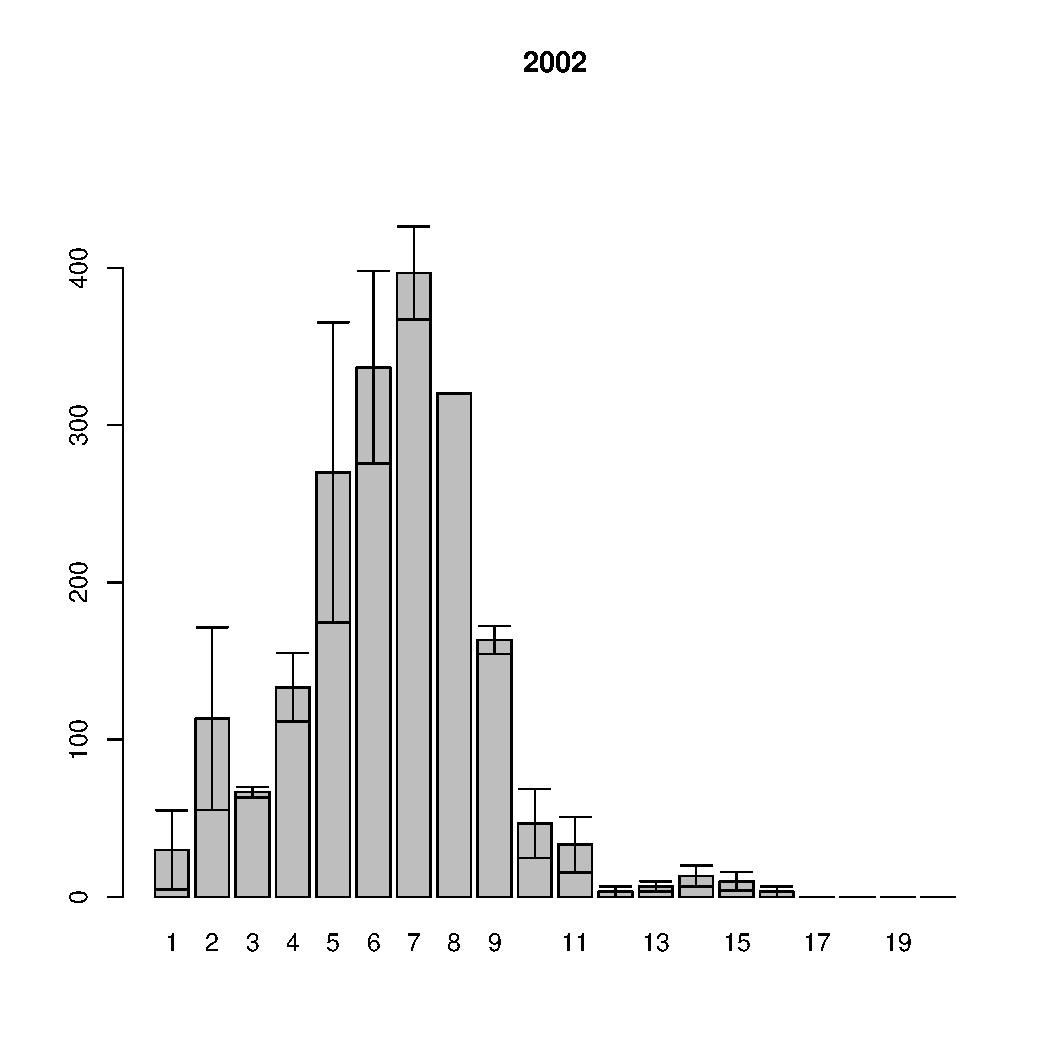
\includegraphics[width=60mm]{../White_Sea/Estuatiy_Luvenga/sizestr_2002_.pdf}
\end{multicols}

%\smallskip

\begin{multicols}{3}
\hfill
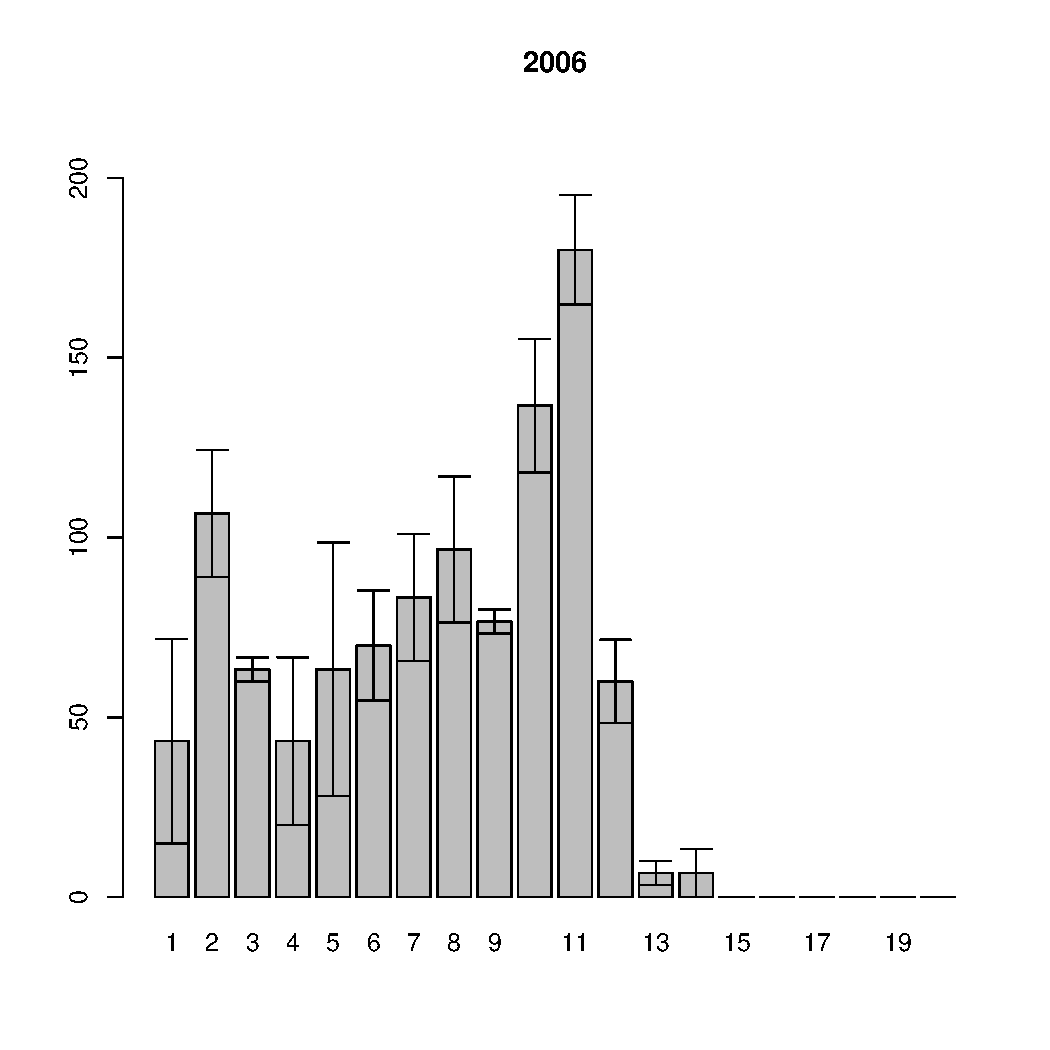
\includegraphics[width=60mm]{../White_Sea/Estuatiy_Luvenga/sizestr_2006_.pdf}
\hfill
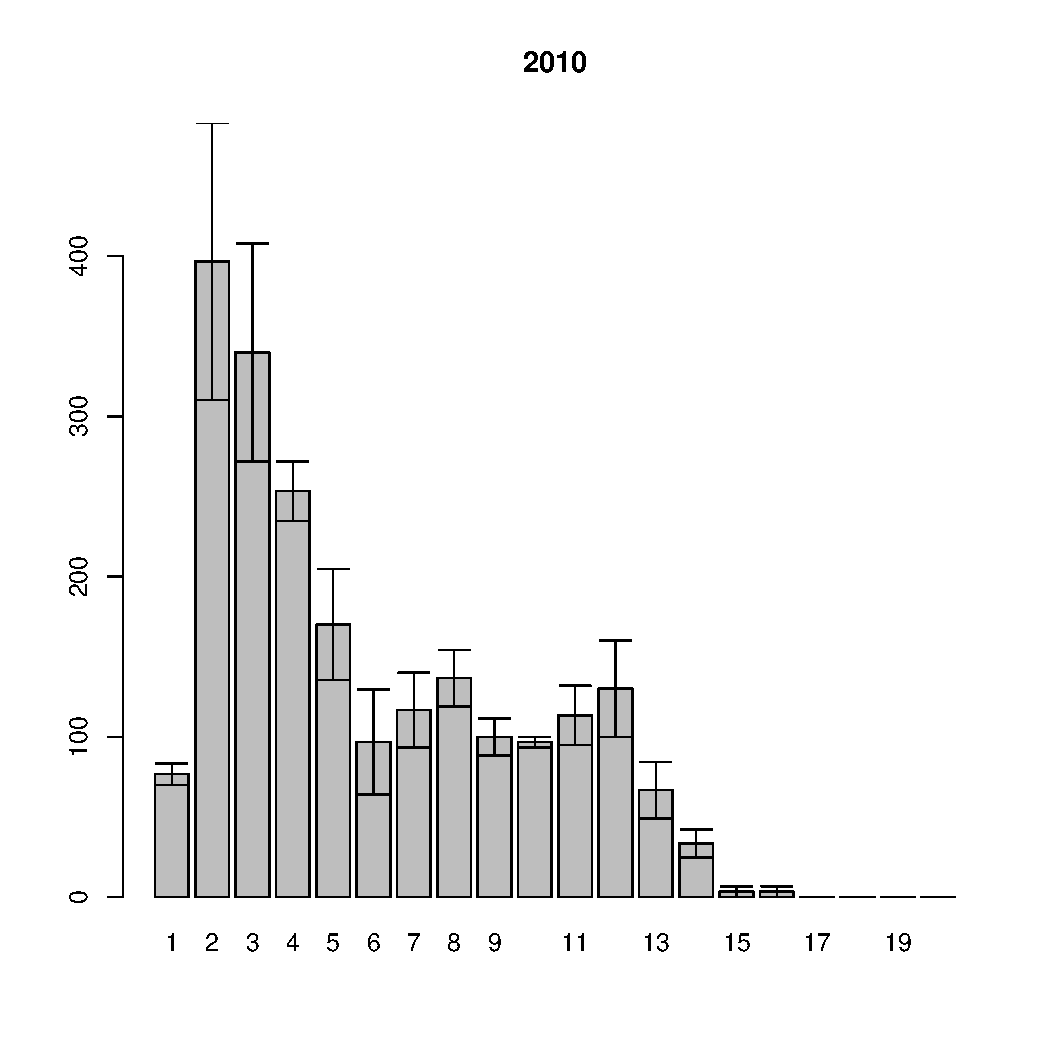
\includegraphics[width=60mm]{../White_Sea/Estuatiy_Luvenga/sizestr_2010_.pdf}
%\hfill
%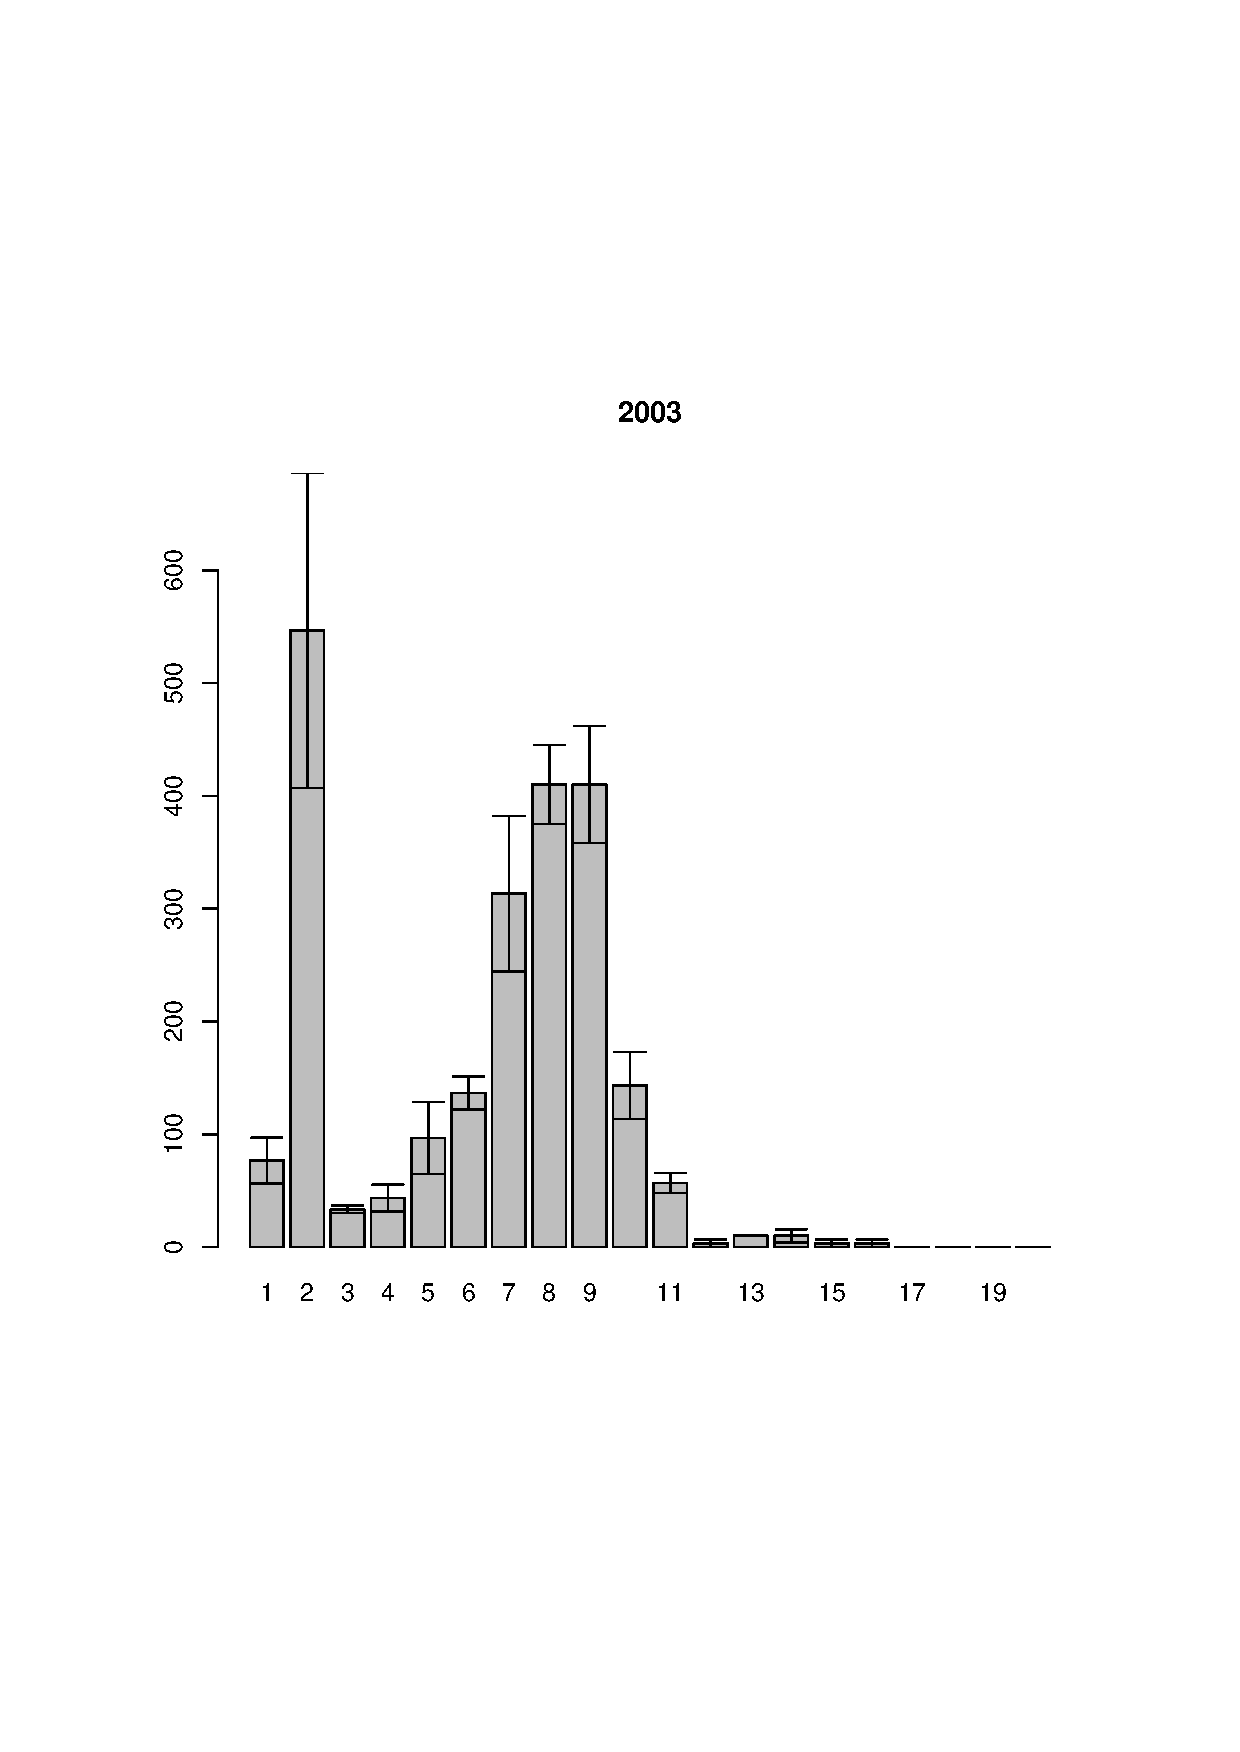
\includegraphics[width=60mm]{../White_Sea/Estuatiy_Luvenga/sizestr_2003_.pdf}
\end{multicols}

%\smallskip

\begin{multicols}{3}
\hfill
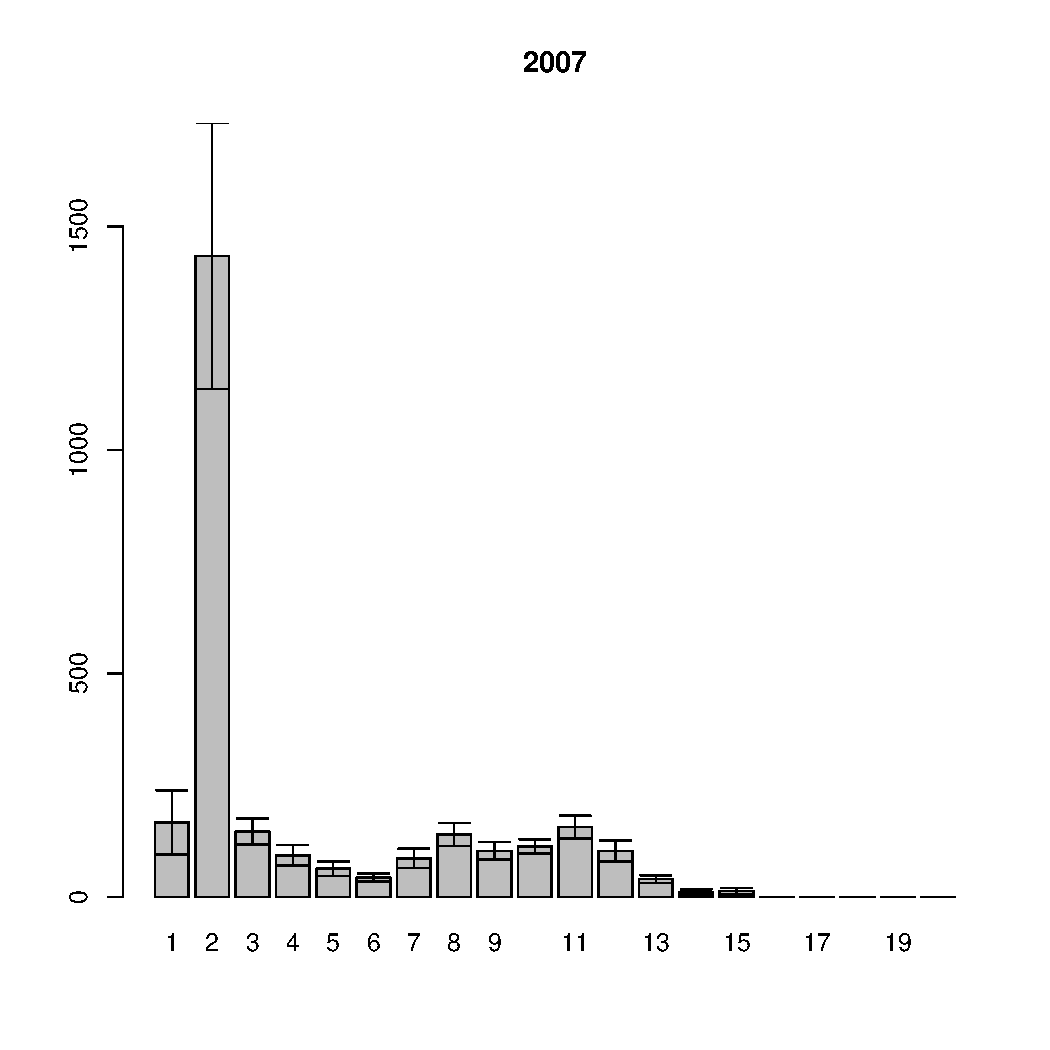
\includegraphics[width=60mm]{../White_Sea/Estuatiy_Luvenga/sizestr_2007_.pdf}
\hfill
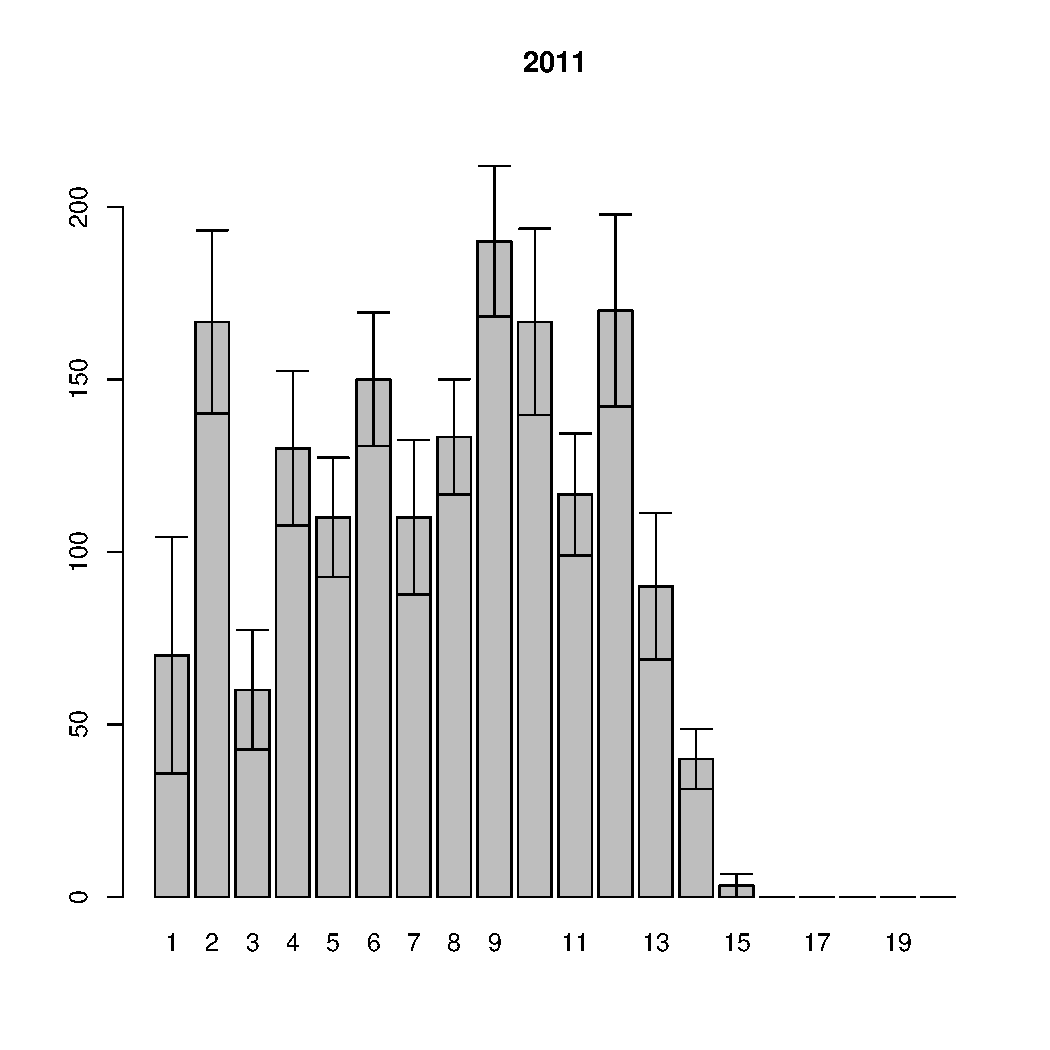
\includegraphics[width=60mm]{../White_Sea/Estuatiy_Luvenga/sizestr_2011_.pdf}
%\hfill
%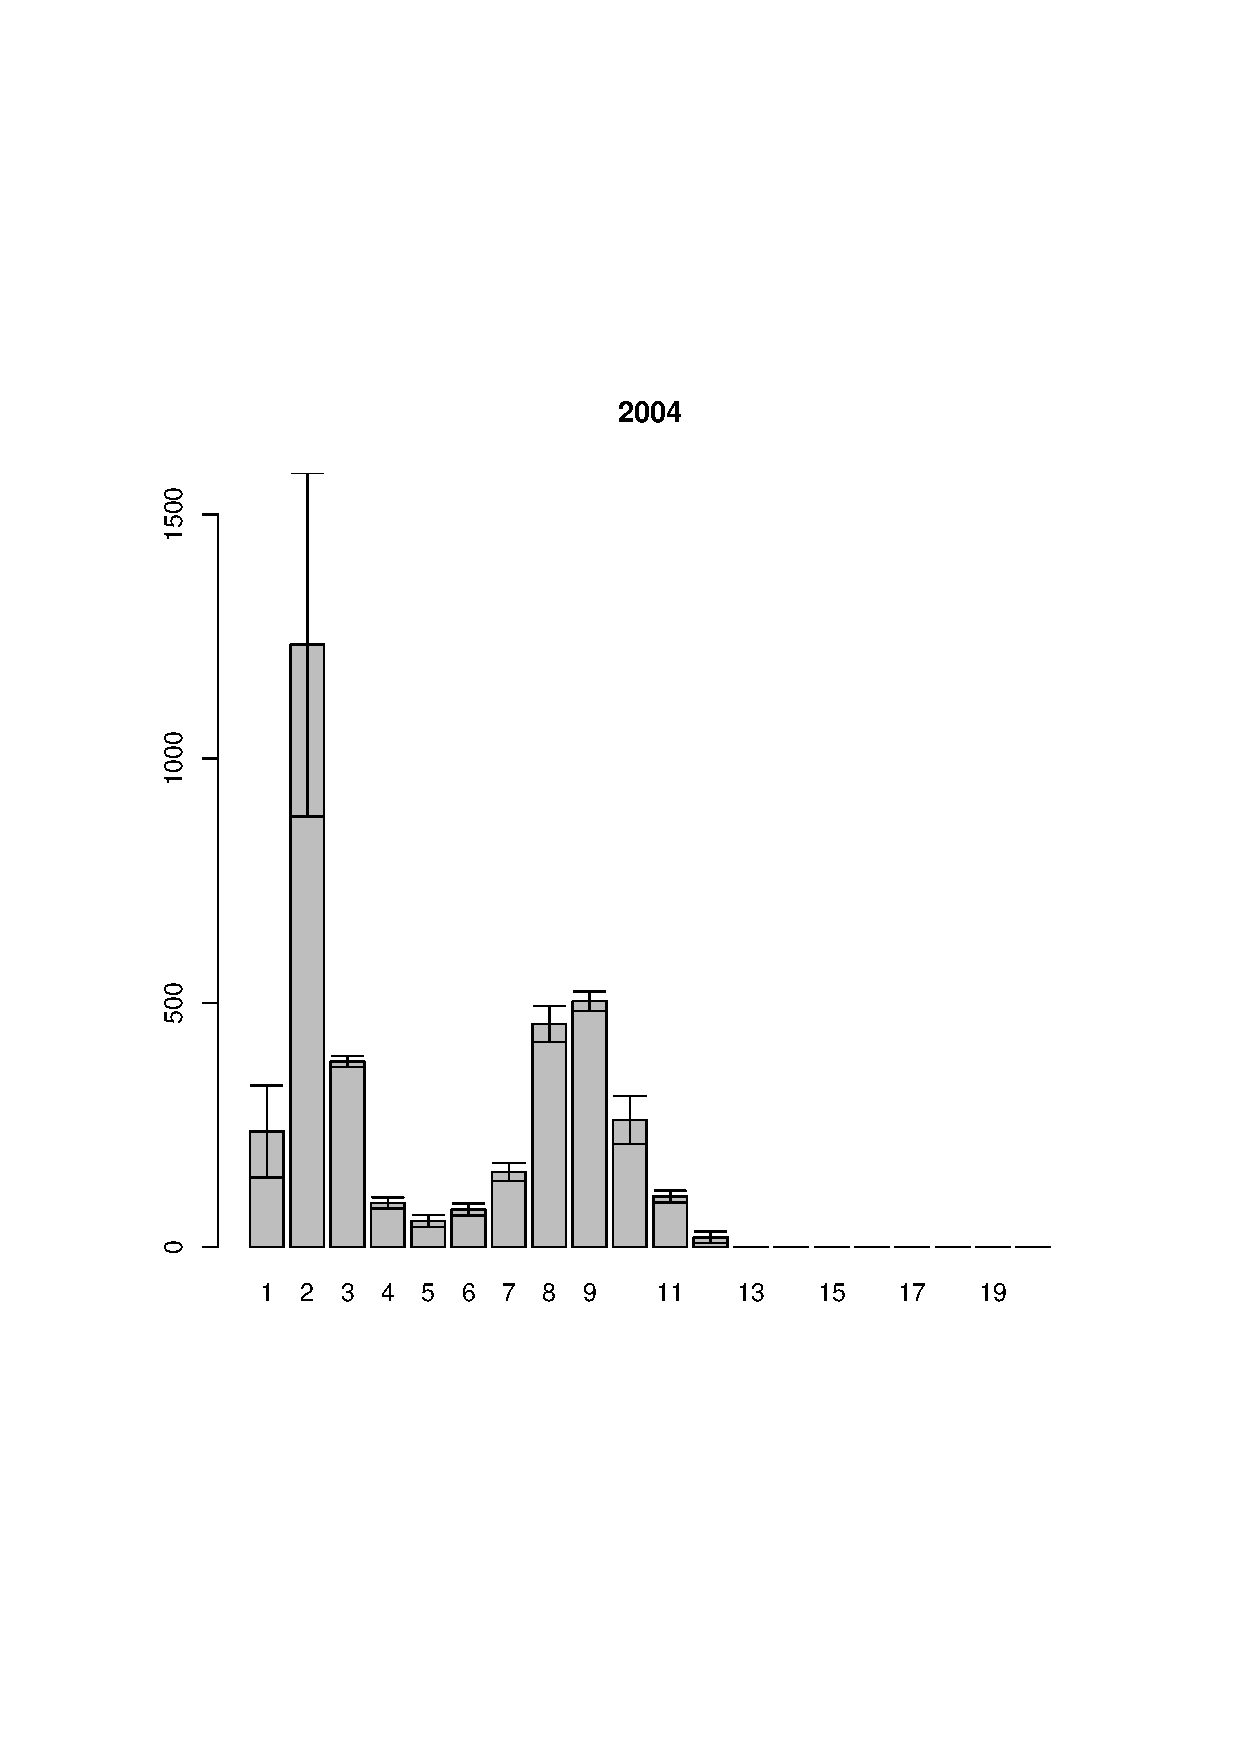
\includegraphics[width=60mm]{../White_Sea/Estuatiy_Luvenga/sizestr_2004_.pdf}
\end{multicols}


%\caption{Размерная структура {\it Macoma balthica} в СГЛ эстуария р. Лувеньги}
%\label{ris:size_str_estuaty_Luv}
\begin{center}
Рис. \ref{ris:size_str_estuary_Luv} (продолжение). Размерная структура {\it Macoma balthica} в СГЛ эстуария р. Лувеньги

\end{center}
\end{figure}

%Горелый Лувеньга
\begin{figure}[h]

\begin{multicols}{3}
\hfill
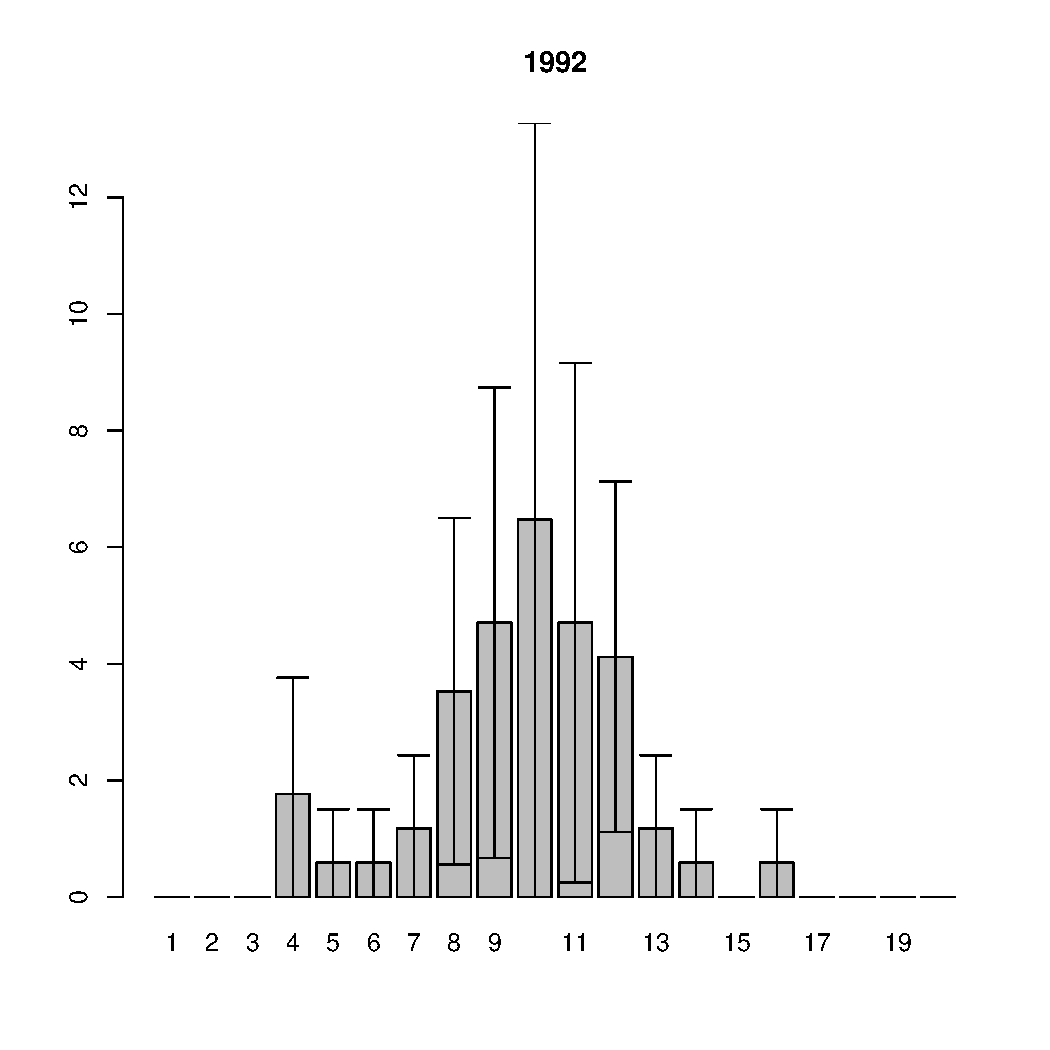
\includegraphics[width=60mm]{../White_Sea/Luvenga_Goreliy/high_1992_.pdf}
\hfill
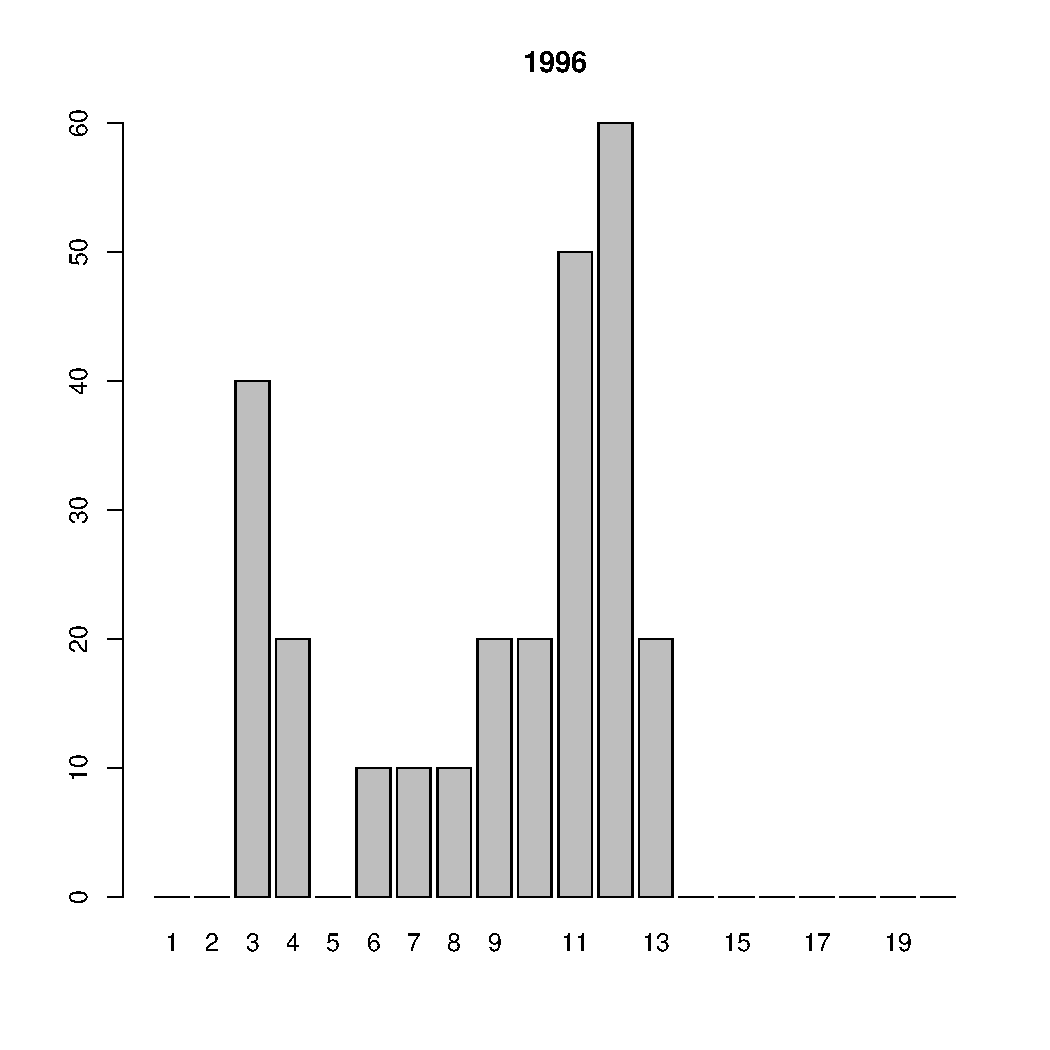
\includegraphics[width=60mm]{../White_Sea/Luvenga_Goreliy/high_1996_.pdf}
\hfill
\includegraphics[width=60mm]{../White_Sea/Luvenga_Goreliy/high_2000_.pdf}
\end{multicols}

%\smallskip


\begin{multicols}{3}
\hfill
\includegraphics[width=60mm]{../White_Sea/Luvenga_Goreliy/high_1993_.pdf}
\hfill
\includegraphics[width=60mm]{../White_Sea/Luvenga_Goreliy/high_1997_.pdf}
\hfill
\includegraphics[width=60mm]{../White_Sea/Luvenga_Goreliy/high_2001_.pdf}
\end{multicols}

%\smallskip

\begin{multicols}{3}
\hfill
\includegraphics[width=60mm]{../White_Sea/Luvenga_Goreliy/high_1994_.pdf}
\hfill
\includegraphics[width=60mm]{../White_Sea/Luvenga_Goreliy/high_1998_.pdf}
\hfill
\includegraphics[width=60mm]{../White_Sea/Luvenga_Goreliy/high_2002_.pdf}
\end{multicols}

%\smallskip

\begin{multicols}{3}
\hfill
\includegraphics[width=60mm]{../White_Sea/Luvenga_Goreliy/high_1995_.pdf}
\hfill
\includegraphics[width=60mm]{../White_Sea/Luvenga_Goreliy/high_1999_.pdf}
\hfill
\includegraphics[width=60mm]{../White_Sea/Luvenga_Goreliy/high_2003_.pdf}
\end{multicols}


\caption{Размерная структура {\it Macoma balthica} в ВГЛ о. Горелого}
\label{ris:size_str_Goreliy_high}
\end{figure}


\begin{figure}[h]

\begin{multicols}{3}
\hfill
\includegraphics[width=60mm]{../White_Sea/Luvenga_Goreliy/high_2004_.pdf}
\hfill
\includegraphics[width=60mm]{../White_Sea/Luvenga_Goreliy/high_2008_.pdf}
\hfill
\includegraphics[width=60mm]{../White_Sea/Luvenga_Goreliy/high_2012_.pdf}
\end{multicols}

%\smallskip


\begin{multicols}{3}
\hfill
\includegraphics[width=60mm]{../White_Sea/Luvenga_Goreliy/high_2005_.pdf}
\hfill
\includegraphics[width=60mm]{../White_Sea/Luvenga_Goreliy/high_2009_.pdf}
%\hfill
%\includegraphics[width=60mm]{../White_Sea/Luvenga_Goreliy/high_2002_.pdf}
\end{multicols}

%\smallskip

\begin{multicols}{3}
\hfill
\includegraphics[width=60mm]{../White_Sea/Luvenga_Goreliy/high_2006_.pdf}
\hfill
\includegraphics[width=60mm]{../White_Sea/Luvenga_Goreliy/high_2010_.pdf}
%\hfill
%\includegraphics[width=60mm]{../White_Sea/Luvenga_Goreliy/high_2003_.pdf}
\end{multicols}

%\smallskip

\begin{multicols}{3}
\hfill
\includegraphics[width=60mm]{../White_Sea/Luvenga_Goreliy/high_2007_.pdf}
\hfill
\includegraphics[width=60mm]{../White_Sea/Luvenga_Goreliy/high_2011_.pdf}
%\hfill
%\includegraphics[width=60mm]{../White_Sea/Luvenga_Goreliy/high_2004_.pdf}
\end{multicols}


%\caption{Размерная структура {\it Macoma balthica} в СГЛ эстуария р. Лувеньги}
%\label{ris:size_str_estuaty_Luv}
\begin{center}
Рис. \ref{ris:size_str_Goreliy_high} (продолжение). Размерная структура {\it Macoma balthica} в ВГЛ о. Горелого

\end{center}
\end{figure}

% Горелый СГЛ
\begin{figure}[h]

\begin{multicols}{3}
\hfill
\includegraphics[width=60mm]{../White_Sea/Luvenga_Goreliy/middle_1992_.pdf}
\hfill
\includegraphics[width=60mm]{../White_Sea/Luvenga_Goreliy/middle_1996_.pdf}
\hfill
\includegraphics[width=60mm]{../White_Sea/Luvenga_Goreliy/middle_2000_.pdf}
\end{multicols}

%\smallskip


\begin{multicols}{3}
\hfill
\includegraphics[width=60mm]{../White_Sea/Luvenga_Goreliy/middle_1993_.pdf}
\hfill
\includegraphics[width=60mm]{../White_Sea/Luvenga_Goreliy/middle_1997_.pdf}
\hfill
\includegraphics[width=60mm]{../White_Sea/Luvenga_Goreliy/middle_2001_.pdf}
\end{multicols}

%\smallskip

\begin{multicols}{3}
\hfill
\includegraphics[width=60mm]{../White_Sea/Luvenga_Goreliy/middle_1994_.pdf}
\hfill
\includegraphics[width=60mm]{../White_Sea/Luvenga_Goreliy/middle_1998_.pdf}
\hfill
\includegraphics[width=60mm]{../White_Sea/Luvenga_Goreliy/middle_2002_.pdf}
\end{multicols}

%\smallskip

\begin{multicols}{3}
\hfill
\includegraphics[width=60mm]{../White_Sea/Luvenga_Goreliy/middle_1995_.pdf}
\hfill
\includegraphics[width=60mm]{../White_Sea/Luvenga_Goreliy/middle_1999_.pdf}
\hfill
\includegraphics[width=60mm]{../White_Sea/Luvenga_Goreliy/middle_2003_.pdf}
\end{multicols}


\caption{Размерная структура {\it Macoma balthica} в СГЛ о. Горелого}
\label{ris:size_str_Goreliy_mid}
\end{figure}


\begin{figure}[h]

\begin{multicols}{3}
\hfill
\includegraphics[width=60mm]{../White_Sea/Luvenga_Goreliy/middle_2004_.pdf}
\hfill
\includegraphics[width=60mm]{../White_Sea/Luvenga_Goreliy/middle_2008_.pdf}
\hfill
\includegraphics[width=60mm]{../White_Sea/Luvenga_Goreliy/middle_2012_.pdf}
\end{multicols}

%\smallskip


\begin{multicols}{3}
\hfill
\includegraphics[width=60mm]{../White_Sea/Luvenga_Goreliy/middle_2005_.pdf}
\hfill
\includegraphics[width=60mm]{../White_Sea/Luvenga_Goreliy/middle_2009_.pdf}
%\hfill
%\includegraphics[width=60mm]{../White_Sea/Luvenga_Goreliy/middle_2002_.pdf}
\end{multicols}

%\smallskip

\begin{multicols}{3}
\hfill
\includegraphics[width=60mm]{../White_Sea/Luvenga_Goreliy/middle_2006_.pdf}
\hfill
\includegraphics[width=60mm]{../White_Sea/Luvenga_Goreliy/middle_2010_.pdf}
%\hfill
%\includegraphics[width=60mm]{../White_Sea/Luvenga_Goreliy/middle_2003_.pdf}
\end{multicols}

%\smallskip

\begin{multicols}{3}
\hfill
\includegraphics[width=60mm]{../White_Sea/Luvenga_Goreliy/middle_2007_.pdf}
\hfill
\includegraphics[width=60mm]{../White_Sea/Luvenga_Goreliy/middle_2011_.pdf}
%\hfill
%\includegraphics[width=60mm]{../White_Sea/Luvenga_Goreliy/middle_2004_.pdf}
\end{multicols}


%\caption{Размерная структура {\it Macoma balthica} в СГЛ эстуария р. Лувеньги}
%\label{ris:size_str_estuaty_Luv}
\begin{center}
Рис. \ref{ris:size_str_Goreliy_mid} (продолжение). Размерная структура {\it Macoma balthica} в СГЛ о. Горелого

\end{center}
\end{figure}

% Горелый midlow


\begin{figure}[h]

\begin{multicols}{3}
\hfill
\includegraphics[width=60mm]{../White_Sea/Luvenga_Goreliy/midlow_1992_.pdf}
\hfill
\includegraphics[width=60mm]{../White_Sea/Luvenga_Goreliy/midlow_1996_.pdf}
\hfill
\includegraphics[width=60mm]{../White_Sea/Luvenga_Goreliy/midlow_2000_.pdf}
\end{multicols}

%\smallskip


\begin{multicols}{3}
\hfill
\includegraphics[width=60mm]{../White_Sea/Luvenga_Goreliy/midlow_1993_.pdf}
\hfill
\includegraphics[width=60mm]{../White_Sea/Luvenga_Goreliy/midlow_1997_.pdf}
\hfill
\includegraphics[width=60mm]{../White_Sea/Luvenga_Goreliy/midlow_2001_.pdf}
\end{multicols}

%\smallskip

\begin{multicols}{3}
\hfill
\includegraphics[width=60mm]{../White_Sea/Luvenga_Goreliy/midlow_1994_.pdf}
\hfill
\includegraphics[width=60mm]{../White_Sea/Luvenga_Goreliy/midlow_1998_.pdf}
\hfill
\includegraphics[width=60mm]{../White_Sea/Luvenga_Goreliy/midlow_2002_.pdf}
\end{multicols}

%\smallskip

\begin{multicols}{3}
\hfill
\includegraphics[width=60mm]{../White_Sea/Luvenga_Goreliy/midlow_1995_.pdf}
\hfill
\includegraphics[width=60mm]{../White_Sea/Luvenga_Goreliy/midlow_1999_.pdf}
\hfill
\includegraphics[width=60mm]{../White_Sea/Luvenga_Goreliy/midlow_2003_.pdf}
\end{multicols}


\caption{Размерная структура {\it Macoma balthica} в поясе фукоидов о. Горелого}
\label{ris:size_str_Goreliy_midlow}
\end{figure}


\begin{figure}[h]

\begin{multicols}{3}
\hfill
\includegraphics[width=60mm]{../White_Sea/Luvenga_Goreliy/midlow_2004_.pdf}
\hfill
\includegraphics[width=60mm]{../White_Sea/Luvenga_Goreliy/midlow_2008_.pdf}
\hfill
\includegraphics[width=60mm]{../White_Sea/Luvenga_Goreliy/midlow_2012_.pdf}
\end{multicols}

%\smallskip


\begin{multicols}{3}
\hfill
\includegraphics[width=60mm]{../White_Sea/Luvenga_Goreliy/midlow_2005_.pdf}
\hfill
\includegraphics[width=60mm]{../White_Sea/Luvenga_Goreliy/midlow_2009_.pdf}
%\hfill
%\includegraphics[width=60mm]{../White_Sea/Luvenga_Goreliy/midlow_2002_.pdf}
\end{multicols}

%\smallskip

\begin{multicols}{3}
\hfill
\includegraphics[width=60mm]{../White_Sea/Luvenga_Goreliy/midlow_2006_.pdf}
\hfill
\includegraphics[width=60mm]{../White_Sea/Luvenga_Goreliy/midlow_2010_.pdf}
%\hfill
%\includegraphics[width=60mm]{../White_Sea/Luvenga_Goreliy/midlow_2003_.pdf}
\end{multicols}

%\smallskip

\begin{multicols}{3}
\hfill
\includegraphics[width=60mm]{../White_Sea/Luvenga_Goreliy/midlow_2007_.pdf}
\hfill
\includegraphics[width=60mm]{../White_Sea/Luvenga_Goreliy/midlow_2011_.pdf}
%\hfill
%\includegraphics[width=60mm]{../White_Sea/Luvenga_Goreliy/midlow_2004_.pdf}
\end{multicols}


%\caption{Размерная структура {\it Macoma balthica} в СГЛ эстуария р. Лувеньги}
%\label{ris:size_str_estuaty_Luv}
\begin{center}
Рис. \ref{ris:size_str_Goreliy_midlow} (продолжение). Размерная структура {\it Macoma balthica} в поясе фукоидов о. Горелого

\end{center}
\end{figure}


% Горелый НГЛ
\begin{figure}[h]

\begin{multicols}{3}
\hfill
\includegraphics[width=60mm]{../White_Sea/Luvenga_Goreliy/low_1992_.pdf}
\hfill
\includegraphics[width=60mm]{../White_Sea/Luvenga_Goreliy/low_1996_.pdf}
\hfill
\includegraphics[width=60mm]{../White_Sea/Luvenga_Goreliy/low_2000_.pdf}
\end{multicols}

%\smallskip


\begin{multicols}{3}
\hfill
\includegraphics[width=60mm]{../White_Sea/Luvenga_Goreliy/low_1993_.pdf}
\hfill
\includegraphics[width=60mm]{../White_Sea/Luvenga_Goreliy/low_1997_.pdf}
\hfill
\includegraphics[width=60mm]{../White_Sea/Luvenga_Goreliy/low_2001_.pdf}
\end{multicols}

%\smallskip

\begin{multicols}{3}
\hfill
\includegraphics[width=60mm]{../White_Sea/Luvenga_Goreliy/low_1994_.pdf}
\hfill
\includegraphics[width=60mm]{../White_Sea/Luvenga_Goreliy/low_1998_.pdf}
\hfill
\includegraphics[width=60mm]{../White_Sea/Luvenga_Goreliy/low_2002_.pdf}
\end{multicols}

%\smallskip

\begin{multicols}{3}
\hfill
\includegraphics[width=60mm]{../White_Sea/Luvenga_Goreliy/low_1995_.pdf}
\hfill
\includegraphics[width=60mm]{../White_Sea/Luvenga_Goreliy/low_1999_.pdf}
\hfill
\includegraphics[width=60mm]{../White_Sea/Luvenga_Goreliy/low_2003_.pdf}
\end{multicols}


\caption{Размерная структура {\it Macoma balthica} в НГЛ о. Горелого}
\label{ris:size_str_Goreliy_low}
\end{figure}


\begin{figure}[h]

\begin{multicols}{3}
\hfill
\includegraphics[width=60mm]{../White_Sea/Luvenga_Goreliy/low_2004_.pdf}
\hfill
\includegraphics[width=60mm]{../White_Sea/Luvenga_Goreliy/low_2008_.pdf}
\hfill
\includegraphics[width=60mm]{../White_Sea/Luvenga_Goreliy/low_2012_.pdf}
\end{multicols}

%\smallskip


\begin{multicols}{3}
\hfill
\includegraphics[width=60mm]{../White_Sea/Luvenga_Goreliy/low_2005_.pdf}
\hfill
\includegraphics[width=60mm]{../White_Sea/Luvenga_Goreliy/low_2009_.pdf}
%\hfill
%\includegraphics[width=60mm]{../White_Sea/Luvenga_Goreliy/low_2002_.pdf}
\end{multicols}

%\smallskip

\begin{multicols}{3}
\hfill
\includegraphics[width=60mm]{../White_Sea/Luvenga_Goreliy/low_2006_.pdf}
\hfill
\includegraphics[width=60mm]{../White_Sea/Luvenga_Goreliy/low_2010_.pdf}
%\hfill
%\includegraphics[width=60mm]{../White_Sea/Luvenga_Goreliy/low_2003_.pdf}
\end{multicols}

%\smallskip

\begin{multicols}{3}
\hfill
\includegraphics[width=60mm]{../White_Sea/Luvenga_Goreliy/low_2007_.pdf}
\hfill
\includegraphics[width=60mm]{../White_Sea/Luvenga_Goreliy/low_2011_.pdf}
%\hfill
%\includegraphics[width=60mm]{../White_Sea/Luvenga_Goreliy/low_2004_.pdf}
\end{multicols}


%\caption{Размерная структура {\it Macoma balthica} в СГЛ эстуария р. Лувеньги}
%\label{ris:size_str_estuaty_Luv}
\begin{center}
Рис. \ref{ris:size_str_Goreliy_low} (продолжение). Размерная структура {\it Macoma balthica} в НГЛ
 о. Горелого

\end{center}
\end{figure}


%II разрез high

\begin{figure}[h]

\begin{multicols}{3}
\hfill
\includegraphics[width=60mm]{../White_Sea/Luvenga_II_razrez/high_beatch_1992_.pdf}
\hfill
\includegraphics[width=60mm]{../White_Sea/Luvenga_II_razrez/high_beatch_1996_.pdf}
\hfill
\includegraphics[width=60mm]{../White_Sea/Luvenga_II_razrez/high_beatch_2000_.pdf}
\end{multicols}

%\smallskip


\begin{multicols}{3}
\hfill
\includegraphics[width=60mm]{../White_Sea/Luvenga_II_razrez/high_beatch_1993_.pdf}
\hfill
\includegraphics[width=60mm]{../White_Sea/Luvenga_II_razrez/high_beatch_1997_.pdf}
\hfill
\includegraphics[width=60mm]{../White_Sea/Luvenga_II_razrez/high_beatch_2002_.pdf}
\end{multicols}

%\smallskip

\begin{multicols}{3}
\hfill
\includegraphics[width=60mm]{../White_Sea/Luvenga_II_razrez/high_beatch_1994_.pdf}
\hfill
\includegraphics[width=60mm]{../White_Sea/Luvenga_II_razrez/high_beatch_1998_.pdf}
\hfill
\includegraphics[width=60mm]{../White_Sea/Luvenga_II_razrez/high_beatch_2004_.pdf}
\end{multicols}

%\smallskip

\begin{multicols}{3}
\hfill
\includegraphics[width=60mm]{../White_Sea/Luvenga_II_razrez/high_beatch_1995_.pdf}
\hfill
\includegraphics[width=60mm]{../White_Sea/Luvenga_II_razrez/high_beatch_1999_.pdf}

\end{multicols}


\caption{Размерная структура {\it Macoma balthica} на верхнем пляже материковой литорали в районе пос.~ Лувеньга}
\label{ris:size_str_2razrez_high}
\end{figure}

% 2razrez fucus
\begin{figure}[h]

\begin{multicols}{3}
\hfill
\includegraphics[width=60mm]{../White_Sea/Luvenga_II_razrez/fucus_zone_1992_.pdf}
\hfill
\includegraphics[width=60mm]{../White_Sea/Luvenga_II_razrez/fucus_zone_1996_.pdf}
\hfill
\includegraphics[width=60mm]{../White_Sea/Luvenga_II_razrez/fucus_zone_2000_.pdf}
\end{multicols}

%\smallskip


\begin{multicols}{3}
\hfill
\includegraphics[width=60mm]{../White_Sea/Luvenga_II_razrez/fucus_zone_1993_.pdf}
\hfill
\includegraphics[width=60mm]{../White_Sea/Luvenga_II_razrez/fucus_zone_1997_.pdf}
\hfill
\includegraphics[width=60mm]{../White_Sea/Luvenga_II_razrez/fucus_zone_2002_.pdf}
\end{multicols}

%\smallskip

\begin{multicols}{3}
\hfill
\includegraphics[width=60mm]{../White_Sea/Luvenga_II_razrez/fucus_zone_1994_.pdf}
\hfill
\includegraphics[width=60mm]{../White_Sea/Luvenga_II_razrez/fucus_zone_1998_.pdf}
\hfill
\includegraphics[width=60mm]{../White_Sea/Luvenga_II_razrez/fucus_zone_2004_.pdf}
\end{multicols}

%\smallskip

\begin{multicols}{3}
\hfill
\includegraphics[width=60mm]{../White_Sea/Luvenga_II_razrez/fucus_zone_1995_.pdf}
\hfill
\includegraphics[width=60mm]{../White_Sea/Luvenga_II_razrez/fucus_zone_1999_.pdf}

\end{multicols}


\caption{Размерная структура {\it Macoma balthica} в поясе фукоидов материковой литорали в районе пос. Лувеньга}
\label{ris:size_str_2razrez_fucus}
\end{figure}

% 2razrez zostera
\begin{figure}[h]

\begin{multicols}{3}
\hfill
\includegraphics[width=60mm]{../White_Sea/Luvenga_II_razrez/zostera_zone_1992_.pdf}
\hfill
\includegraphics[width=60mm]{../White_Sea/Luvenga_II_razrez/zostera_zone_1996_.pdf}
\hfill
\includegraphics[width=60mm]{../White_Sea/Luvenga_II_razrez/zostera_zone_2000_.pdf}
\end{multicols}

%\smallskip


\begin{multicols}{3}
\hfill
\includegraphics[width=60mm]{../White_Sea/Luvenga_II_razrez/zostera_zone_1993_.pdf}
\hfill
\includegraphics[width=60mm]{../White_Sea/Luvenga_II_razrez/zostera_zone_1997_.pdf}
\hfill
\includegraphics[width=60mm]{../White_Sea/Luvenga_II_razrez/zostera_zone_2002_.pdf}
\end{multicols}

%\smallskip

\begin{multicols}{3}
\hfill
\includegraphics[width=60mm]{../White_Sea/Luvenga_II_razrez/zostera_zone_1994_.pdf}
\hfill
\includegraphics[width=60mm]{../White_Sea/Luvenga_II_razrez/zostera_zone_1998_.pdf}
\hfill
\includegraphics[width=60mm]{../White_Sea/Luvenga_II_razrez/zostera_zone_2004_.pdf}
\end{multicols}

%\smallskip

\begin{multicols}{3}
\hfill
\includegraphics[width=60mm]{../White_Sea/Luvenga_II_razrez/zostera_zone_1995_.pdf}
\hfill
\includegraphics[width=60mm]{../White_Sea/Luvenga_II_razrez/zostera_zone_1999_.pdf}

\end{multicols}


\caption{Размерная структура {\it Macoma balthica} в поясе взморника {\it Zostera marina} материковой литорали в районе пос. Лувеньга}
\label{ris:size_str_2razrez_zostera}
\end{figure}

% 2razrez low
\begin{figure}[h]

\begin{multicols}{3}
\hfill
\includegraphics[width=60mm]{../White_Sea/Luvenga_II_razrez/low_beatch_1992_.pdf}
\hfill
\includegraphics[width=60mm]{../White_Sea/Luvenga_II_razrez/low_beatch_1996_.pdf}
\hfill
\includegraphics[width=60mm]{../White_Sea/Luvenga_II_razrez/low_beatch_2000_.pdf}
\end{multicols}

%\smallskip


\begin{multicols}{3}
\hfill
\includegraphics[width=60mm]{../White_Sea/Luvenga_II_razrez/low_beatch_1993_.pdf}
\hfill
\includegraphics[width=60mm]{../White_Sea/Luvenga_II_razrez/low_beatch_1997_.pdf}
\hfill
\includegraphics[width=60mm]{../White_Sea/Luvenga_II_razrez/low_beatch_2002_.pdf}
\end{multicols}

%\smallskip

\begin{multicols}{3}
\hfill
\includegraphics[width=60mm]{../White_Sea/Luvenga_II_razrez/low_beatch_1994_.pdf}
\hfill
\includegraphics[width=60mm]{../White_Sea/Luvenga_II_razrez/low_beatch_1998_.pdf}

\end{multicols}

%\smallskip

\begin{multicols}{3}
\hfill
\includegraphics[width=60mm]{../White_Sea/Luvenga_II_razrez/low_beatch_1995_.pdf}
\hfill
\includegraphics[width=60mm]{../White_Sea/Luvenga_II_razrez/low_beatch_1999_.pdf}

\end{multicols}


\caption{Размерная структура {\it Macoma balthica} на нижнем пляже материковой литорали в районе пос. Лувеньга}
\label{ris:size_str_2razrez_low}
\end{figure}



%ЮГ Ряшкова
\begin{figure}[h]

\begin{multicols}{3}
\hfill
\includegraphics[width=60mm]{../White_Sea/Ryashkov_YuG/YuG_2001_.pdf}
\hfill
\includegraphics[width=60mm]{../White_Sea/Ryashkov_YuG/YuG_2005_.pdf}
\hfill
\includegraphics[width=60mm]{../White_Sea/Ryashkov_YuG/YuG_2009_.pdf}
\end{multicols}

%\smallskip


\begin{multicols}{3}
\hfill
\includegraphics[width=60mm]{../White_Sea/Ryashkov_YuG/YuG_2002_.pdf}
\hfill
\includegraphics[width=60mm]{../White_Sea/Ryashkov_YuG/YuG_2006_.pdf}
\hfill
\includegraphics[width=60mm]{../White_Sea/Ryashkov_YuG/YuG_2010_.pdf}
\end{multicols}

%\smallskip

\begin{multicols}{3}
\hfill
\includegraphics[width=60mm]{../White_Sea/Ryashkov_YuG/YuG_2003_.pdf}
\hfill
\includegraphics[width=60mm]{../White_Sea/Ryashkov_YuG/YuG_2007_.pdf}
\hfill
\includegraphics[width=60mm]{../White_Sea/Ryashkov_YuG/YuG_2011_.pdf}
\end{multicols}

%\smallskip

\begin{multicols}{3}
\hfill
\includegraphics[width=60mm]{../White_Sea/Ryashkov_YuG/YuG_2004_.pdf}
\hfill
\includegraphics[width=60mm]{../White_Sea/Ryashkov_YuG/YuG_2008_.pdf}
\hfill
\includegraphics[width=60mm]{../White_Sea/Ryashkov_YuG/YuG_2012_.pdf}
\end{multicols}


\caption{Размерная структура {\it Macoma balthica} у нуля глубин в Южной губе о. Ряшкова}
\label{ris:size_str_YuG}
\end{figure}


%Западная Ряшкова Салма
\begin{figure}[h]

\begin{multicols}{3}
\hfill
\includegraphics[width=60mm]{../White_Sea/Ryashkov_ZRS/zrs_1994_.pdf}
\hfill
\includegraphics[width=60mm]{../White_Sea/Ryashkov_ZRS/zrs_1998_.pdf}
\hfill
\includegraphics[width=60mm]{../White_Sea/Ryashkov_ZRS/zrs_2002_.pdf}
\end{multicols}

%\smallskip


\begin{multicols}{3}
\hfill
\includegraphics[width=60mm]{../White_Sea/Ryashkov_ZRS/zrs_1995_.pdf}
\hfill
\includegraphics[width=60mm]{../White_Sea/Ryashkov_ZRS/zrs_1999_.pdf}
\hfill
\includegraphics[width=60mm]{../White_Sea/Ryashkov_ZRS/zrs_2003_.pdf}
\end{multicols}

%\smallskip

\begin{multicols}{3}
\hfill
\includegraphics[width=60mm]{../White_Sea/Ryashkov_ZRS/zrs_1996_.pdf}
\hfill
\includegraphics[width=60mm]{../White_Sea/Ryashkov_ZRS/zrs_2000_.pdf}
\hfill
\includegraphics[width=60mm]{../White_Sea/Ryashkov_ZRS/zrs_2004_.pdf}
\end{multicols}

%\smallskip

\begin{multicols}{3}
\hfill
\includegraphics[width=60mm]{../White_Sea/Ryashkov_ZRS/zrs_1997_.pdf}
\hfill
\includegraphics[width=60mm]{../White_Sea/Ryashkov_ZRS/zrs_2001_.pdf}
\hfill
\includegraphics[width=60mm]{../White_Sea/Ryashkov_ZRS/zrs_2005_.pdf}
\end{multicols}


\caption{Размерная структура {\it Macoma balthica} в СГЛ Западной Ряшковой салмы}
\label{ris:size_str_ZRS}
\end{figure}



\begin{figure}[h]

\begin{multicols}{3}
\hfill
\includegraphics[width=60mm]{../White_Sea/Ryashkov_ZRS/zrs_2006_.pdf}
\hfill
\includegraphics[width=60mm]{../White_Sea/Ryashkov_ZRS/zrs_2010_.pdf}
\hfill

\end{multicols}

%\smallskip


\begin{multicols}{3}
\hfill
\includegraphics[width=60mm]{../White_Sea/Ryashkov_ZRS/zrs_2007_.pdf}
\hfill
\includegraphics[width=60mm]{../White_Sea/Ryashkov_ZRS/zrs_2011_.pdf}
\hfill

\end{multicols}

%\smallskip

\begin{multicols}{3}
\hfill
\includegraphics[width=60mm]{../White_Sea/Ryashkov_ZRS/zrs_2008_.pdf}
\hfill
\includegraphics[width=60mm]{../White_Sea/Ryashkov_ZRS/zrs_2012_.pdf}
\hfill

\end{multicols}

%\smallskip

\begin{multicols}{3}
\hfill
\includegraphics[width=60mm]{../White_Sea/Ryashkov_ZRS/zrs_2009_.pdf}
\hfill
%\includegraphics[width=60mm]{../White_Sea/Ryashkov_ZRS/zrs_2012_.pdf}
%\hfill

\end{multicols}


%\caption{Размерная структура {\it Macoma balthica} в СГЛ Западной Ряшковой салмы}
%\label{ris:size_str_ZRS}
\begin{center}
Рис.\ref{ris:size_str_ZRS} (продолжение). Размерная структура {\it Macoma balthica} в СГЛ Западной Ряшковой салмы
\end{center}
\end{figure}

%Ломнишный

\begin{figure}[h]

\begin{multicols}{2}
\hfill
\includegraphics[width=65mm]{../White_Sea/Lomnishniy/Lomnishniy_2007_.pdf}
\hfill
\includegraphics[width=65mm]{../White_Sea/Lomnishniy/Lomnishniy_2010_.pdf}
\end{multicols}

%\smallskip


\begin{multicols}{2}
\hfill
\includegraphics[width=65mm]{../White_Sea/Lomnishniy/Lomnishniy_2008_.pdf}
\hfill
\includegraphics[width=65mm]{../White_Sea/Lomnishniy/Lomnishniy_2011_.pdf}
\end{multicols}

%\smallskip

\begin{multicols}{2}
\hfill
\includegraphics[width=65mm]{../White_Sea/Lomnishniy/Lomnishniy_2009_.pdf}
\hfill
\includegraphics[width=65mm]{../White_Sea/Lomnishniy/Lomnishniy_2012_.pdf}
\end{multicols}

%\smallskip


\caption{Размерная структура {\it Macoma balthica} у нуля глубин литорали о.Ломнишный}
\label{ris:size_str_Lomnishniy}
\end{figure}


\end{document}

\afterpage{\clearpage}

	\section{Размерная структура {\it Macoma balthica}}

		\subsection{Белое море}

	\subsubsection{Эстуарий реки Лувеньги}
На данном участке размерную структуру поселения маком в среднем горизонте литорали (СГЛ) отслеживали на протяжении $20$~лет ($1992 - 2012$).
За все время наблюдения максимальная длина особи, отмеченная в поселении составляла $18$~мм.

Характер размерно-частотного распределения особей неоднократно менялся на протяжении периода наблюдений (приложение~\ref{app:White_sizestr_hist}, рис.~\ref{ris:size_str_estuary_Luv}).
С $1993$ до $1997$ года в размерной структуре поселения выделялось три модальных класса, причем за все $5$~лет один из них попадал на особей до $4$~мм , второй на $7 - 9$ мм и третий --- это особи длиной более $10$~мм. 
В $1998$ году размерная структура поселения стала мономодальной, так как практически не осталось крупных особей, но
появилось много моллюсков длиной $1-2$~мм. 
В дальнейшем до $2002$ года оставалось мономодальное распределение особей по размерам, и происходило смещение модального класса --- в $2002$ году это были особи размером $6-7$ мм. 

В $2003$ году можно было выделить два пика: моллюски длиной $1-2$ мм и $7-9$~мм, то есть размерная структура поселения вновь стала бимодальной. 
В дальнейшем до $2012$~года размерная структура маком в данном поселении остается бимодальной. 
Первый модальный класс сохраняется --- особи длиной $1-2$~мм, а второй модальный класс варьирует, его составляют в разные годы особи длиной от $9$ до $12$~мм.
Количественное соотношение особей двух модальных классов менялось. Чаще ($2004$, $2007 - 2010$~ года) преобладали мелкие моллюски, но в отдельные годы ($2006$, $2012$) доля крупных была выше, либо представительство крупных и мелких доминирующих классов было сравнимым ($2005$, $2011$~годы).



			\subsubsection{Остров Горелый}

На данном участке размерную структуру поселения маком отслеживали на протяжении $20$~лет ($1992 - 2012$) в пределах трех горизонтов литорали и у нуля глубин.
За все время наблюдения максимальная длина особи, отмеченная в поселении составляла $20$~мм.

В верхнем горизонте литорали (ВГЛ) размерная структура поселения до $1997$ года (приложение~\ref{app:White_sizestr_hist}, рис.~\ref{ris:size_str_Goreliy_high}) представляла собой бимодальное распределение с модальными классами $2-5$~мм и $7-13$~мм.
В $1998$ году появилось значительное количество особей длиной $1-4$~мм. 
В дальнейшем можно было наблюдать смещение по оси размеров данного модального класса. 
В $2001$ году в поселении вновь сформировалась бимодальная размерная структура (модальные классы $1-3$ и $5-6$ мм), и в дальнейшем такое распределение сохранялось до $2007$ года.
В $2008 - 2009$ годах распределение было мономодальное с модальным классом $1-2$~мм.
Интересно отметить, что с $2002$ по $2009$ год доминирующим размерным классом в поселении были особи длиной $1-2$~мм.
В $2011-2012$ году восстановилась бимодальная размерная структура с модальными классами $1-4$ и $9-11$~мм.

%\bigskip
В среднем горизонте литорали (СГЛ) до $1996$ года в этой зоне выделялась бимодальная размерная структура (приложение~\ref{app:White_sizestr_hist}, рис.~\ref{ris:size_str_Goreliy_mid}) (модальные классы --- моллюски длиной $1-4$~мм и $6-13$~мм). 
В $1997$ году распределение было практически равномерное при общей низкой численности. 
В $1998$ году появилось значительное количество моллюсков длиной до $1$ мм. 
После чего наблюдалось смещение модального класса до $2003$ года. 
До $2001$ года размерная структура поселения оставалась мономодальной, но в $2002-03$ годах появился еще один модальный класс -- моллюски длиной до $2$ мм. 
Таким образом, после $2002$ года  в поселении вновь восстановилась бимодальная размерная структура, которая сохраняется вплоть до $2007$ года.
В $2008$ году распределение особей по размерам становится мономодальным за счет элиминирования особей крупных размеров. 
В $2011-2012$ году восстанавливается бимодальное распределение.


%\bigskip
В нижнем горизонте литорали (НГЛ) в $1992$ году в связи с малой численностью моллюсков сложно говорить о характерной размерной структуре поселения (приложение~\ref{app:White_sizestr_hist}, рис.~\ref{ris:size_str_Goreliy_midlow}).
В $1993$ году фактически можно выделить только один пик ($2-3$~мм), хотя и было очень незначительное повышение при длине $9-10$~мм. 
Но с $1994$ по $1996$ год было представлено бимодальное распределение с модальными классами $1-3$ мм и $9-11$~мм.
В $1997$ году численность моллюсков значительно снизилась, и распределение по размерам было практически равномерное. 
В $1998-1999$ году в значительных количествах появились особи длиной $2-3$~мм и можно было наблюдать смещение модального класса по оси размеров вплоть до $2003$ года, когда его значение становится $5-6$~мм. 
Кроме того, с $2002$ года можно было выделить еще один модальный класс -- особи длиной $1-2$~мм, то есть размерная структура поселения вновь стала бимодальной, каковой и оставалась до конца периода наблюдений.


%\bigskip
У нуля глубин в $1992$ году моллюсков практически не было (приложение~\ref{app:White_sizestr_hist}, рис.~\ref{ris:size_str_Goreliy_low}), но в $1993$ году можно говорить о бимодальной размерной структуре поселения, которая сохранялась до $1997$ года. 
В $1998-1999$ году произошло элиминирование крупных особей на фоне появления значительного количества особей длиной $1-2$~мм. 
В $2001-2003$ годах в поселении восстановилась бимодальная структура и в $2003$ году модальные классы образовывали особи длиной до $1$ мм и $8.1-9.0$ мм. 
С $2003$ до $2007$ года преобладали особи длиной $9-12$~мм, а с $2008$ появляется второй модальный пик --- особи размером $1-3$~мм.


		\subsubsection*{Материковая литораль в районе поселка Лувеньга}
На данном участке размерную структуру поселения маком отслеживали на протяжении $10$~лет ($1992 - 2004$) в пределах четырех биотопов.
За все время наблюдения максимальная длина особи, отмеченная в поселении составляла $24$~мм.

В зоне верхнего пляжа размерная структура поселения (приложение~\ref{app:White_sizestr_hist}, рис.~\ref{ris:size_str_2razrez_high}) в $1993$ году была мономодальная, но с $1994$ по $1997$ годы стала бимодальной с модальными классами $2-5$ и $6-10$~мм.
В $1998$ году появилось значительное число особей размером менее $1$ мм, после чего до $2002$ года прослеживалось смещение модального класса. 
В $2002$ году в поселении восстановилась бимодальная структура (модальные классы -- $1-2$ мм и $5-6$ мм).

%\bigskip
В поясе фукоидов размерная структура поселения (приложение~\ref{app:White_sizestr_hist}, рис.~\ref{ris:size_str_2razrez_fucus}) в $1992-1997$ году характеризовалась наличием двух модальных классов: $1-6$ и $7-12$~мм. 
С $1998$ по $2000$ года размерная структура поселения была мономодальной, причем все $3$ года пик формировали особи длиной $1-2$~мм. 
В $2002$ году вновь выделялось два модальных класса: $1-2$ и $7-8$~мм.

%\bigskip
В поясе зостеры до $1998$ года в размерной структуре поселения пояса зостеры выделялись незначительные пики и можно говорить о равномерном распределении моллюсков(приложение~\ref{app:White_sizestr_hist}, рис.~\ref{ris:size_str_2razrez_zostera}). 
После $1998$ года она стала мономодальной, причем пик формировали моллюски длиной $1-2$ мм.


%\bigskip
В зоне нижнего пляжа до $1999$ года размерная структура поселения была полимодальная, хотя эти пики нельзя было четко выделить (приложение~\ref{app:White_sizestr_hist}, рис.~\ref{ris:size_str_2razrez_low}). 
В $1999-2000$ годах практически не осталось крупных особей, но появилось значительное число моллюсков размером $1-2$~мм. 

		\subsubsection{Южная губа о.~Ряшкова}

На данном участке наблюдения проводили с $2001$ года, размерную структуру поселения у нуля глубин отслеживали в течение $12$ лет.
Максимальный размер маком в данном поселении составил $23$~мм в $2003$ году, однако в другие годы максимальный размер не превышал $16$~мм.

В Южной губе на протяжении всего периода наблюдений размерная структура (приложение~\ref{app:White_sizestr_hist}, рис.~\ref{ris:size_str_YuG}) поселения была мономодальной с преобладанием особей длиной $1-3$~мм. 



		\subsubsection{Западная Ряшкова салма}

На литорали о.~Ряшкова в Западной Ряшковой салме наблюдения проводили с $1994$ по $2012$ год ($18$~лет). Наблюдения проводили в среднем горизонте литорали.
Максимальный размер моллюсков, отмеченный в поселении составил $20$~мм.

На данном участке  до $1998$ года размерная структура была полимодальной(приложение~\ref{app:White_sizestr_hist}, рис.~\ref{ris:size_str_ZRS}). 
В $1999$ году крупные особи в основном элиминировали, и размерная структура стала мономодальной с доминированием моллюсков длиной $1-2$~мм.
В дальнейшем $2001$ года до конца наблюдений размерная структура была бимодальной с модальными классами $1-3$ и $9-11$~мм.


		\subsubsection{о.~Ломнишный}

На литорали острова Ломнишный наблюдения проводили с $2007$ года в течение $6$~лет у нуля глубин. 
Максимальный размер особи, отмеченный в поселении составлял $17$~мм.

Размерная структура на данном участке в течение всего периода наблюдений была мономодальной (приложение~\ref{app:White_sizestr_hist}, рис.~\ref{ris:size_str_Lomnishniy}).
В основном доминировали особи длиной $1-3$~мм, за исключением $2009-2010$ годов, когда доминировали особи длиной $5$ и $7$~мм, соответсвенно.


\bigskip
Таким образом, наиболее распростарненный вариант динамики размерной структуры в поселениях {\it M.~balthica} в Белом море это чередование бимодальной и мономодальной размерных структур.
Мономодальная структура обычно формируется на фоне практически полной элиминации крупных особей при пополнении поселения новой генерацией маком.
В дальнейшем, если новое пополнение происходит быстрее, чем предыдущая генерация элиминирует, то формируется бимодальная размерная структура.

Среди 6 мониторинговых участков в Кандалакшском заливе Белого моря для двух из них --- в Южной губе острова Ряшков и на о. Ломнишный --- динамика размерной структуры принципиально отличалась, и мы ежегодно видим мономодальное распределение особей по размерам с доминированием молоди.

\afterpage{\clearpage}

		\subsection{Баренцево море}

		\subsubsection{Губы Кольского залива}

На участке Абрам-мыс (рис.~\ref{ris:Barents_sizestr}) были представлены особи длиной от $2$ до $16$~мм. 
В среднем горизонте литорали характер распределения был мономодальный с преобладанием моллюсков длиной $10-13$~мм. 
В нижнем горизонте литорали к аналогичному пику (особи длной $12-14$~мм) добавляется второй — моллюски длиной $2-3$~мм.

На участке в Пала-губе (рис.~\ref{ris:Barents_sizestr}) также в среднем горизонте распределение особей по размерам было мономодальным, а на нижнем --- бимодальным. 
Однако при этом наблюдалась обратная ситуация: в среднем горизонте литорали доминировали особи самой мелкой размерной группы --- $3-4$~мм, в то время как  в нижнем горизонте кроме таких особей  хорошо представлена размерная группа $10-12$~мм.

		\subsubsection{Губы побережья Восточного Мурмана}

В губе Гаврилово (прил.~\ref{app:Barents_sizestr_hist}, рис.~\ref{ris:Barents_sizestr}) распределение особей практически равномерное. 
В среднем горизонте литорали несколько преобладают особи длиной $15-20$~мм. 
В нижнем горизонте литорали представлены лишь единичные особи различных возрастов.	

Во всех горизонтах губы Ярнышной (прил.~\ref{app:Barents_sizestr_hist}, рис.~\ref{ris:Barents_sizestr}) доминировали особи длиной $4-6$~мм. 
На всех участках можно отметить присутствие относительно крупных моллюсков (особи длиной более $14$~мм), однако их представленность на порядок варьирует в разных горизонтах.

В губе Шельпино (прил.~\ref{app:Barents_sizestr_hist}, рис.~\ref{ris:Barents_sizestr})  представлены единичные особи длиной от $6$ до $16$~мм. 
В среднем горизонте литорали некоторое превышение формируют особи длиной $15$~мм, однако и они остаются немногочисленны.

В губе Порчниха (прил.~\ref{app:Barents_sizestr_hist}, рис.~\ref{ris:Barents_sizestr}) были представлены особи длиной от $4$ до $21$~мм. 
Распределение особей по размерам было полимодальным. 
Выделяется по крайней мере три моды: $4-7$~мм, $9-12$~мм и $18-20$~мм. 
Несущественное превышение численности  отмечено для особей длиной $13-15$~мм.

В губе Ивановская (прил.~\ref{app:Barents_sizestr_hist}, рис.~\ref{ris:Barents_sizestr}) были обнаружены макомы длиной от $2$ до $13$~мм. 
Количество особей в каждой размерной группе колебалось от $20$ до $30$ экзмепляров, лишь моллюсков длиной $2$~мм было отмечено около $50$. 
Распределение особей по размерам было практически равномерным при некотором превышении доли особей длиной $2$ и $10$~мм. 

		\subsubsection{Дальний пляж губы Дальнезеленецкой (Восточный Мурман)}
На данном участке ни в один год в пробах не было отмечено особей {\it M.~balthica} с длиной раковины менее $2$~мм (прил.~\ref{app:Barents_sizestr_hist}, рис.~\ref{ris:size_str_DZ}). 
Максимальный размер моллюсков в разные годы колебался от $18$ до $20$~мм. 

С $2002$ до $2004$ года размерная структура маком в данном поселении была полимодальной. 
Можно говорить по крайней мере о трех модальных группах.
Доминировали все эти годы особи размером $8 - 14$~мм.
В $2005$ году размерная структура фактически мономодальная с преобладанием крупных особей длиной больше $12$~мм, и встречаются единичные моллюски размером $3 - 4$~мм.
В $2006$ году добавляется вторая модальная группа~--- особи длиной $3 - 5$~мм.
После $2007$ года восстанавливается полимодальное распределение особей по размерам.


\bigskip

Таким образом, на исследованных участках был представлены все возможные варианты рамерной структуры: мономодальное (участки: Арабм-мыс СГЛ, Пала-губа СГЛ, губа Гаврилово СГЛ), бимодальное (участки: Абрам-мыс НГЛ, Пала-губа НГЛ, губа Ярнышная, губа Дальне-Зеленецкая СГЛ, губа Порчниха СГЛ) и практически равномерное (участки: губа Гаврилово НГЛ, губа Дальне-Зеленецкая ВГЛ и НГЛ, губа Шельпино ВГЛ и СГЛ, губа Ивановская ВСЛ) распределение особей по размерам. 

Мономодальное распределение особей по размерам наблюдается либо при доминировании мелких особей длиной $3-5$~мм, либо при доминировании крупных --- $12-18$~мм.
При бимодальном распределении обычно первую моду формировали мелкие макомы длиной $2-5$~мм, а вторую --- моллюски длиной более $10$~мм.

\afterpage{\clearpage}

\afterpage{\clearpage}

%%рост в разных условиях
    \chapter{Линейный рост {\it Macoma balthica}}
Рост особей рассматривается как отклик особей на совокупность условий обитания. 
Анализ роста проводили по усредненным возрастным рядам. 
Для их получения по каждому описанию   были   построены   треугольные   матрицы   (табл.~\ref{tab:Abram_sgl_growth_matrix}~--~\ref{tab:Porchnikha_sgl_growth_matrix},   Приложение~\ref{app:growth_matrix}),   полностью описывающие рост особей в поселении.

В   первую   очередь   анализ   был   проведен   по  усредненным   возрастным   рядам, построенным как взвешенная оценка (с учетом числа особей) характера роста всех генераций по   результатам   измерений   размеров  моллюсков  в   периоды   зимней   остановки   роста.  
Такая кумулятивная   характеристика   должна   в   наибольшей   мере   отражать   особенности   условий роста маком в каждом местообитании.
Наиболее длинный возрастной ряд удалось получить для среднего горизонта литорали губы Гаврилово --- $15$~лет при длине $17,9$~мм (табл.~\ref{tab:Gavrilovo_sgl_growth_matrix},   Приложение~\ref{app:growth_matrix}). 
Однако максимальный размер особей был отмечен в верхнем горизонте литорали губы Ярнышная --- $20,1$~мм при возрасте $13$~лет (табл.~\ref{tab:Yarnyshnaya_sgl_growth_matrix},   Приложение~\ref{app:growth_matrix}). 

Полученные   возрастные   ряды   были   аппроксимированы   с   помощью   уравнения Берталанфи   (рис.~\ref{ris:Barents_growth_gorizonts_all}).
    \begin{figure}[p]
        \includegraphics[width=\textwidth]{../Barenc_Sea/growth_from_MSc/Rost_gorizonts_all.jpg}
    \caption{Разнообразие моделей линейного роста, описывающих взвешенные характеристики возрастных рядов генераций в изученных поселениях маком}
    \label{ris:Barents_growth_gorizonts_all}
    \end{figure}

Быстрее   всего   росли   макомы   в   среднем   горизонте   литорали   губы Порчниха, достигая длины $19,4$~мм за $9$~лет и в среднем горизонте литорали губы Ярнышная --- $16,7$~мм за $8$~лет. 
Остальные кривые не распадаются на очевидные группы, и некоторые пересекают   друг   друга.   
Поэтому   была   использована   формальная   процедура   сравнения полученных   кривых   роста   с   учетом   разброса   эмпирических   данных   относительно регрессионной модели (рис.~\ref{ris:dendrogramma_linear_all_gorizonts}).
    \begin{figure}[p]
        \includegraphics[width=\textwidth]{../Barenc_Sea/growth_from_MSc/dendrogramma_sravnenie_rosta_linear_all_gorizonts.jpg}
    \caption{Классификация поселений маком по моделям линейного роста, описывающих взвешенные характеристики возрастных рядов генераций}
    \label{ris:dendrogramma_linear_all_gorizonts}
    \end{figure}

В   ходе   классификации   было   выделено   три   кластера.   
В   первый   вошли   следующие описания (уровень различий внутри кластера менее $0,87$): Абрам-мыс, Пала-губа НГЛ, губа Гаврилово   СГЛ,   губа   Ярнышная   НГЛ,   Шельпино   ВГЛ.   
Второй   кластер   (уровень   различий внутри кластера менее $0,76$) составили участки Пала-губа СГЛ, губа Гаврилово НГЛ, губа Дальнезеленецкая,   губа   Ярнышная   ВГЛ,   Шельпино   СГЛ.   
В   последний   кластер   (уровень различий внутри кластера менее $0,38$) вошли участки губа Ярнышная СГЛ и губа Порчниха СГЛ. 

На участках Абрам-мыс и губа Дальнезеленецкая характер роста был одинаковый на всех горизонтах литорали. 
Однако в распределении остальных описаний нет географической приуроченности. 
Как и ожидалось, поселения  из средних горизонтов литорали губы Ярнышной и губы Порчниха   выделились   в   отдельный   кластер.   
Низкий   уровень   различий   ($0,38$)   говорит   о большом   разбросе   наблюдаемых   значений   относительно   модели   роста.   
Это   могло   бы свидетельствовать   об   относительно   грубом   описании   соответствующих   возрастных   рядов, хотя   значительный объем  выборки ($76$  и $65$  особей, соответственно)  позволяет  говорить  о значительном варьировании роста маком в пределах каждого участка.

Интересно,   что   при   незначительном   расхождении   кривых   роста,   уровень   различий между первым и вторым кластером оказался очень высоким ($2,52$). 
Не было отмечено явного разделения участков по мареографическому уровню, хотя во второй кластер попало больше описаний   с   более   высоких   горизонтов   литорали.   Максимальное   различие   было   между кластерами $2$ и $3$ ($2,76$).

По   итогам   классификации   было   выделено   три   группы   маком,   отличающиеся   по характеру роста (рис.~\ref{ris:Barents_clusters_gorizonts_all}).
    \begin{figure}[p]
        \includegraphics[width=\textwidth]{../Barenc_Sea/growth_from_MSc/rost_clusters_all.jpg}
    \caption{Модели роста, передающие  принципиальные свойства вариации характера линейного роста маком в изученных местообитаниях}
    \label{ris:Barents_clusters_gorizonts_all}
    \end{figure}
Первая группа — особи с наименьшей скоростью роста достигали длины $16,4$ мм за $14$ лет, обитавшие на относительно более низком уровне осушки. 
Макомы с промежуточной   скоростью   роста   вырастали   за   $13$   лет   $до   19,3$   мм.   
Особи   с   максимальной скоростью роста за $9$ лет достигали длины $18$ мм.

Таким   образом,   не   удалось   выделить   ни   географической,   ни   мареографической приуроченности особей с одинаковой скоростью роста. 
Возможно, это связано с тем, что во взвешенных оценках возрастных рядов могут сильнее проявиться черты нехарактерных, но сильно   представленных   в   поселении   сегодня   генераций,   и,   следовательно,   в   каждом возрастном   ряду   получается   разная   представленность   межгодовой   составляющей   условий 
роста маком. 

Для   того,   чтобы   снять   эти   влияния,   следующий   анализ   проводили   с   купированием исходных  данных  до  объединения   нескольких  описаний возрастных рядов  только  старших (>8+) генераций (рис.~\ref{ris:Barents_growth_gorizonts_8year}).
    \begin{figure}[p]
        \includegraphics[width=\textwidth]{../Barenc_Sea/growth_from_MSc/Rost_8+_gorizonts.jpg}
        \caption{Разнообразие моделей линейного роста, описывающих усредненные возрастные ряды генераций маком старше 8 лет} 
    \label{ris:Barents_growth_gorizonts_8year}
    \end{figure}
Полученная   картина   аналогична   полученной   по   интегральным   описаниям:   быстрее всего росли макомы в среднем горизонте литорали губы Порчниха и в среднем горизонте литорали губы Ярнышная, в то время как остальные кривые не распадаются на очевидные группы, и некоторые пересекают друг друга. 
Однако при сравнении полученных кривых роста с учетом разброса эмпирических данных относительно регрессионной модели было выделено 4 кластера (рис.~\ref{ris:dendrogramma_linear_clusters_8year}).
    \begin{figure}[p]
        \includegraphics[width=\textwidth]{../Barenc_Sea/growth_from_MSc/dendrogramma_sravnenie_rosta_linear_8year_gorizonts.jpg}
        \caption{Классификация поселений маком по моделям линейного роста, описывающих усредненные возрастные ряды генераций маком старше 8 лет}
    \label{ris:dendrogramma_linear_clusters_8year}
    \end{figure}

В первый кластер (уровень различий внутри кластера менее $0,86$) вошли следующие описания:  Абрам-мыс, Пала-губа НГЛ, губа  Гаврилово  СГЛ, губа Ярнышная НГЛ. 
Второй кластер (уровень различий внутри кластера менее $0,57$) составили участки Пала-губа СГЛ, губа Гаврилово НГЛ, губа Дальнезеленецкая, губа Ярнышная ВГЛ, Шельпино СГЛ. 
В третий кластер (уровень различий внутри кластера менее $0,61$) вошли участки губа Ярнышная СГЛ и губа Порчниха СГЛ. 
В отдельный кластер попал участок губа Шельпино ВГЛ (минимальное различие $2,53$ --- с кластером $1$). 
Таким   образом,   единственное   качественное   изменение   относительно   результатов, полученных при сравнении усредненных кривых роста --- это выделение верхнего горизонта литорали губы Шельпино в отдельный кластер. 
Однако, коэффициенты различия значительно изменились. 
В два раза увеличилось различие между описаниями внутри кластера $3$, различие внутри кластера $2$ уменьшились. 
Максимальное различие было отмечено между кластерами два и три ($5,1$).

По итогам классификации было выделено четыре группы маком, отличающиеся по характеру роста (рис. \ref{ris:Barents_clusters_gorizonts_8year}). 
    \begin{figure}[p]
        \includegraphics[width=\textwidth]{../Barenc_Sea/growth_from_MSc/Rost_8+_clusters.jpg}
        \caption{Модели роста, передающие  принципиальные свойства вариации характера  линейного роста маком старше 8 лет в изученных местообитаниях}
    \label{ris:Barents_clusters_gorizonts_8year}
    \end{figure}
Особи с минимальной скоростью роста ($14$~мм за $12$~лет) обитали в верхнем горизонте литорали губы Шельпино.
Среди групп с промежуточной скоростью роста более   низкой   скоростью   роста   ($16,4$~мм   за   $14$~лет)   обладали   моллюски,   обитавшие   на относительно более низком уровне осушки. 
Особи с максимальной скоростью роста за $9$ лет достигали длины $18$ мм.

Использование   интегральных   моделей   роста   маком   вполне   отвечает   задаче сравнительного анализа их поселений. 
Однако скорость роста моллюсков зависит не только от внешних,   общих   для   всего   поселения,   факторов,   но   и   от   локальных   микроусловий.      
Материалы   настоящей   работы   не   позволяют   нам   провести   анализ   вариации индивидуальных   особенностей   роста   маком   как   отклика   на   условия   их   роста.   
Для   этого нужны специальные экспериментальные исследования. 
Однако можно попытаться выделить групповые   эффекты.   
Речь   идет   о   снижении   уровня   рассматриваемой   биосистемы   до возрастной группы. 

В таблицах приложения~\ref{app:growth_matrix} приведены усредненные для каждой возрастной группы результаты измерений  расстояния  от верхушки раковины до каждой метки  зимней остановки роста.
Используем их для анализа характера вариации средних величин годового прироста. 
Величины годового прироста варьировали от $0,05$ до $3,58$ мм (табл.~\ref{tab:godovoy_prirost_min_max}).
\begin{table}[p]
    \caption{Размах варьирования годового прироста {\it Macoma balthica} в зависимости от участка, горизонта     литорали и начального размера особи}
    \label{tab:godovoy_prirost_min_max}
    \begin{tabularx}{\textwidth}{|lX|XX|XX|XX|XX|}
        \hline
        Участок        &         & \multicolumn{8}{c|}{начальный размер}                                             \\ \cline{3-10}
                              &                 & \multicolumn{2}{c|}{$< 3$ мм} & \multicolumn{2}{c|}{$3-6$ мм} & \multicolumn{2}{c|}{$6-9$ мм} &\multicolumn{2}{c|}{$> 9$ мм}\\ \hline
     \multicolumn{2}{|r|}{годовой прирост}&  мин              & макс   & мин    & макс              & мин  & макс & мин  & макс \\ \hline
        Абрам-мыс      & сгл             & 0,69             & 1,68   & 0,69   & 1,31              & 0,73 & 1,57 & 1,00 & 1,23 \\
                       &  нгл            & 0,90            & 1,77             & 0,88   & 1,48   & 0,80              & 1,73 & 0,67 & 1,50 \\ \hline
        Пала-губа      & сгл             & 0,77             & 2,15   & 1,20   & 2,90              & 1,05 & 1,68 & 1,40 & 1,40 \\
                       & нгл            & 1,01            & 1,43             & 1,01   & 1,86   & 0,83              & 1,73 & 0,85 & 0,85 \\ \hline
        губа Гаврилово & сгл             & 0,70             & 2,10   & 0,93   & 2,40              & 0,80 & 2,10 & 0,70 & 1,75 \\
                       &  нгл            & 0,60            & 2,30             & 1,00   & 2,20   & 0,80              & 2,10 & 0,60 & 1,90 \\ \hline
        губа Ярнышная  & сгл             & 1,08             & 3,30   & 1,80   & 3,58              & 2,60 & 2,75 & 1,22 & 2,52 \\
                       &  нгл            & 0,80            & 1,60             & 0,80   & 1,50   & 0,95              & 1,56 & 0,05 & 1,72 \\   \hline
    \end{tabularx}
\end{table}

В качестве переменных воздействия в контексте данной работы логично обратиться к  таким   причинам   вариации   скорости   маком   как   география   положения   местообитаний, мареография положения станций наблюдений. 
Кроме того, нельзя не учесть очевидную связь величины годового прироста маком с их возрастом. 

В   проведенном   выше   сравнительном   анализе   интегральных   кривых   роста   мы выравнивали эмпирические возрастные ряды с помощью линейной модификации уравнения роста Берталанфи. 
При этом очевидным образом снижается объективность представлений о межгодовых различиях годовых приростов особей в возрастных группах. 
Попробуем отойти от возраста как от условия, организующего скорость роста маком, и в качестве одного из предикторов   величины   годового   прироста   возьмём   начальный   (к   данному   годовому интервалу) средний размер особей возрастной группы.  
Такой анализ логично провести с помощью дисперсионного анализа. 

%из статьи
На первом этапе анализа (факторы <<горизонт литорали>>, <<начальный средний размер особей в возрастной группе>>) установлено (табл.~\ref{tab:prirost_ANOVA_tidal}), что каждая из назначенных причин вариации достоверно определяет величину годового прироста. 
\begin{table}[p]
    \caption{Структура вариансы средних величин годового прироста {\it M. balthica} в возрастных группах в градиентах величины начального среднего размера особей в возрастной группе и мареографического уровня положения станций наблюдения}
    \label{tab:prirost_ANOVA_tidal}
    \begin{center}
    \begin{tabular}{|l|rrrrr|}
    \hline
    Источник вариации & $SS$   & $\nu$   & $M_S$   & $F$     & $\alpha$     \\ \hline
    A                 & 4,74   & 3   & 1,58 & 4,2   & 0,006 \\
    B                 & 11,98  & 2   & 5,99 & 15,92 & 0     \\
    AB                & 2,75   & 6   & 0,46 & 1,22  & 0,295 \\
    W                 & 193,82 & 515 & 0,38 &       &       \\ \hline
\end{tabular}
\end{center}

    \footnotesize{Источники вариации: А --- величины начального среднего размера особей в возрастной группе (4 градации размерных классов),\\ 
    В --- мареографический уровень положения станций наблюдения (три градации)\\
    W --- внутригрупповая вариация.\\
    $SS$ --- общий квадрат, $\nu$ --- степень свободы, $M_S$ --- средний квадрат (варианса), $F$ --- значение статистики Фишера, $\alpha$ --- уровень значимости критерия.}
\end{table}
Весьма примечательно, что при этом наибольшая доля вариации величин годового прироста определяется не начальным размером маком ($SS = 4,74$), а мареографическим уровнем положения станции ($SS = 11,98$).
При анализе структуры вариансы исходного комплекса в градиентах начального среднего размера особей в возрастной группе и географии местообитаний выяснилось, что достоверное влияние на величину среднего годового прироста маком оказывают также оба фактора (табл.~\ref{tab:prirost_ANOVA_geography}).
\begin{table}[p]
    \caption{Структура вариансы средних величин годового прироста {\it M. balthica} в возрастных группах в градиентах величины начального среднего размера особей в возрастной группе и географического положения участка наблюдений}
    \label{tab:prirost_ANOVA_geography}
    \begin{center}
    \begin{tabular}{|l|rrrrr|}
        \hline
    Источник вариации & $SS$   & $\nu$   & $M_S$   & $F$     & $\alpha$     \\ \hline
        A                 & 8,23   & 2   & 4,12 & 13,14 & 0,000003 \\
        C                 & 14,44  & 5   & 2,89 & 9,22  & 0        \\
        AC                & 14,16  & 17  & 0,83 & 2,66  & 0,000351 \\
        W                 & 156,62 & 500 & 0,31 &       &         \\ \hline
    \end{tabular}
\end{center}

    \footnotesize{Источники вариации: А --- величины начального среднего размера особей в возрастной группе (4 градации размерных классов),\\ 
        C --- географическое положение участка наблюдений (6 градаций)\\
    W --- внутригрупповая вариация.\\
    $SS$ --- общий квадрат, $\nu$ --- степень свободы, $M_S$ --- средний квадрат (варианса), $F$ --- значение статистики Фишера, $\alpha$ --- уровень значимости критерия.}
\end{table}
Причем и в этом случае наибольшая доля вариации обусловлена не начальным размером раковины, а фактором <<участок>> ($SS = 14,44$).
Общим для проведенных вариантов двухфакторного дисперсионного анализа оказалось, что в обоих случаях внутригрупповая вариация на порядок превышает факторную составляющую. 
Это говорит о том, что основной причиной вариации величины годового прироста маком в изученных акваториях является крайняя степень разнокачественности особей в местообитаниях. 
%Такая разнокачественность очевидна уже по величине размаха вариации длины раковины маком в возрастных группах (см. табл. 1).
В качестве рабочей гипотезы можно предположить, что в краевой части ареала резкой дифференциации особей {\it M. balthica} по скорости роста могут способствовать любые проявления микрорельефной гетеротопности локальных местообитаний.
Полученные положительные итоги дисперсионного анализа интересно визуализировать для выявления характера мареографического и географического трендов в изменении величины годового прироста маком. 
Для этого представим итоги двухфакторных дисперсионных анализов в виде соответствующих поверхностей отклика.
Весьма показательно, что величины годового прироста маком по мере увеличения начального среднего размера особей в возрастных группах меняются куполообразно (рис.~\ref{ris:prirost_otklik}). 
	\begin{figure}[p]
		\begin{minipage}[b]{.5\linewidth}
		%Фигурка в первом ряду слева размер отведенный под весь этот объект -- 0.46 от ширины строки
		%Параметр [b] означает, что выравнивание этих министраниц будет по нижнему краю
			\begin{center}
				{\small А}
				\includegraphics[width=70mm]{../Barenc_Sea/growth_from_MSc/prirost_otklik_mareography.jpg}
			\end{center}
		\end{minipage}
	\hfil %Это пружинка отодвигающая рисунки друг от друга
		\begin{minipage}[b]{.5\linewidth}
			\begin{center}
				{\small B}
				\includegraphics[width=70mm]{../Barenc_Sea/growth_from_MSc/prirost_otklik_geography.jpg}
			\end{center}
		\end{minipage}
	\caption{Характер изменений средней величины годового прироста особей {\it Macoma balthica} возрастной группы в зависимости от начальной средней длины их раковин, мареографического уровня обитания (A) и условного смещения участка по побережью Мурмана на восток (B)}
\footnotesize{Примечания: Участки: 1 --- Абрам-мыс, 2 --- Пала-губа, 3 --- Гаврилово, 4 --- Ярнышная, 5 --- Дальнезеленецкая, 6 --- Шельпино, 7 --- Порчниха\\
ВГЛ --- верхний горизонт литорали, СГЛ --- средний горизонт литорали, НГЛ --- нижний горизонт литорали}
	\label{ris:prirost_otklik}
	\end{figure}
Во всех исследованных поселениях максимальный прирост наблюдается у особей размерного класса $6 - 9$~мм. 
Таким образом, в изученных поселениях максимальную скорость роста следует ожидать у маком среднего возраста (размера). 
Совершенно неожиданным для нас было явление макcимальной скорости роста маком не в нижнем, а в среднем горизонте осушной зоны (см. рис.~\ref{ris:prirost_otklik}, А). 
%По-видимому, в условиях Мурмана фактор осушки начинает оказывать заметное влияние на скорость роста маком только в верхнем горизонте литорали. 
%Причины снижения скорости роста маком в условиях нижнего горизонта литорали на данном этапе исследований нам не ясны.

\bigskip
Таким образом, на литорали Баренцева моря особи \textit{M.~balthica} гетерогенны по скорости роста.
При сравнении кривых роста не было отмечено сходства роста у особей из одного поселения или с одного уровня осушки. 
Однако анализ среднего годового прироста в различных размерных группах показал, что в более восточных поселениях данный показатель выше, чем в более западных.
Также было показано, что в среднем горизонте литорали средний годовой прирост оказывается выше, чем в верхнем и нижнем.
Данные закономерности были выражены в разной степени у особей, отличающихся по длине раковины.
Во всех случаях наибольший средний годовой прирост наблюдали у особей с длиной раковины $6 - 9$~мм.

\afterpage{\clearpage}

\afterpage{\clearpage}

%%динамика популяций
% для компиляции в lualatex!!
\documentclass[12pt, a4paper]{article}
\usepackage[english,russian]{babel}
\usepackage[warn]{mathtext}
%\usepackage[T2A]{fontenc}
%\usepackage[utf8]{inputenc}

\usepackage{xecyr} % Продукт Вашего покорного слуги ;)

\setmainfont{DejaVu Serif}

\usepackage{color}
\usepackage{amssymb,amsmath}
\usepackage{graphicx}
\usepackage{multicol}

\textheight=24cm           % высота текста
\textwidth=16cm            % ширина текста
\oddsidemargin=0pt         % отступ от левого края
\topmargin=-1.5cm          % отступ от верхнего края
\parindent=24pt            % абзацный отступ
\parskip=0pt               % интервал между абзацами
\tolerance=2000            % терпимость к "жидким" строкам
\flushbottom               % выравнивание высоты страниц
%\def\baselinestretch{1.5} % печать с большим интервалом

%\title{}
%\author{\copyright~~С.А.~Назарова \thanks{e-mail:~sophia.nazarova@gmail.com}}
%\date{}

\begin{document}
\begin{figure}[h]

\begin{multicols}{2}
\hfill
\includegraphics[width=65mm]{../White_Sea/Luvenga_Goreliy/N_dynamic.pdf}
\hfill
\includegraphics[width=65mm]{../White_Sea//Luvenga_II_razrez/N_dynamic.pdf}
\end{multicols}

%\smallskip


\begin{multicols}{2}
\hfill
\includegraphics[width=65mm]{../White_Sea/Estuatiy_Luvenga/N_dynamic.pdf}
\hfill
\includegraphics[width=65mm]{../White_Sea/Ryashkov_ZRS/N_dynamic.pdf}
\end{multicols}

%\smallskip

\begin{multicols}{2}
\hfill
\includegraphics[width=65mm]{../White_Sea/Ryashkov_YuG/N_dynamic.pdf}
\hfill
\includegraphics[width=65mm]{../White_Sea/Lomnishniy/N_dynamic.pdf}
\end{multicols}

%\smallskip


\caption{Динамика плотности поселений {\it Macoma balthica} в вершине Кандалакшского залива}
\label{ris:dynamic_Kandalaksha_all}
\end{figure}


\begin{figure}[h]

\begin{multicols}{2}
\hfill
\includegraphics[width=65mm]{../White_Sea/Luvenga_Goreliy/N2_dynamic.pdf}
\hfill
\includegraphics[width=65mm]{../White_Sea//Luvenga_II_razrez/N2_dynamic.pdf}
\end{multicols}

%\smallskip


\begin{multicols}{2}
\hfill
\includegraphics[width=65mm]{../White_Sea/Estuatiy_Luvenga/N2_dynamic.pdf}
\hfill
\includegraphics[width=65mm]{../White_Sea/Ryashkov_ZRS/N2_dynamic.pdf}
\end{multicols}

%\smallskip

\begin{multicols}{2}
\hfill
\includegraphics[width=65mm]{../White_Sea/Ryashkov_YuG/N2_dynamic.pdf}
\hfill
\includegraphics[width=65mm]{../White_Sea/Lomnishniy/N2_dynamic.pdf}
\end{multicols}

%\smallskip


\caption{Динамика численности {\it Macoma balthica} с длиной раковины более $1$~мм в поселениях вершины Кандалакшского залива}
\label{ris:dynamic_Kandalaksha_all}
\end{figure}

\end{document}

%%
	\subsection{Анализ динамики численности {\it Macoma balthica} в Кандалакшском заливе Белого моря}
При изучении динамики численности можно анализировать несколько компонентов.
Первый компонент --- наличие или отсутсвие тренда как направленноого изменения численности.
При убирании тренда остается компонент динамики, для которого двумя крайими случаями будет: стабильная численность, которая поддерживается за счет плотностнозависимых процессов как систем обраной связи и неконтролируемый рост численности популяции по экспоненте.

Мы проанализировали динамику численности {\it M.~balthica} на каждом участке на наличие тренда при помощи теста Мантеля (табл.~\ref{tab:Mantel_N2_trend}).
	\begin{table}[ht]
	\caption{Выявление трендов в динамике численности {\it Macoma balthica} на различных участках Белого моря.}
	\label{tab:Mantel_N2_trend}
        \begin{tabular}{|p{0.25\textwidth}|*{2}{p{0.2\textwidth}|p{0.25\textwidth}|}} \hline
	Участок & $Mantel$ & $p$ & наличие тренда
	\\ \hline
	Эстуарий р. Лувеньга & 0,3168 & 0,003 & есть
	\\ \hline
	о. Горелый & 0,0269 & 0,368 & нет
	\\ \hline
	материковая литораль (Лувеньга) & 0,6103 & 0,001 & есть
	\\ \hline
	Южная губа о. Ряшков & 0,3687 & 0,015 & есть
	\\ \hline
	Запдная Ряшкова салма & 0,0108 & 0,404 & нет
	\\ \hline
	Ломнишный & -0,0999 & 0,47 & нет
	\\ \hline
	г. Медвежья & 0,0154 & 0,385 & нет
	\\ \hline
	г. Сельдяная & 0,2524 & 0,003 & есть
	\\ \hline
	\end{tabular}
	%    {\footnotesize Примечание: достоверность различий *** \textemdash $p<0,001$; ** \textemdash $p<0,05$; * \textemdash $p<0,1$.}
	\end{table}

Было показано наличие тренда на 4 участках: эстуарий р.~Лувеньга, материковая литораль в районе пос. Лувеньга, Южная губа о.~Ряшкова, г. Сельдяная.
Для удаления тренда из исходных значений были вычтены предсказанные значения из регрессионной модели $N = a + b*T$, где $N$ --- численность, экз./м$^2$, $T$ --- годы.
По детрендированному ряду были рассчитаны частные автокорреляции ($PRCF$ - partial rate correlation function).  
Коррелограммы представлены на рисунке \ref{ris:perm_PRCF_Kandalaksha_N2_detrend}.
	\begin{figure}[ht]
	
	\begin{minipage}[b]{.46\linewidth}
	%Фигурка в первом ряду слева размер отведенный под весь этот объект \textendash 0.46 от ширины строки
	%Параметр [b] означает, что выравнивание этих министраниц будет по нижнему краю
	\begin{center}
	{\footnotesize Эстуарий р.~Лувеньги}
		\includegraphics[width=65mm]{../White_Sea/dynamic_N_N1/perm_PRCF_Estuary_detrend.pdf}

	\end{center}
	\end{minipage}
		\hfil %Это пружинка отодвигающая рисунки друг от друга
	\begin{minipage}[b]{.46\linewidth}
%Следующий рисунок - первый ряд справа %DUNGEON S_4 \ AB
	\begin{center}
	{\footnotesize о.~Горелый}
		\includegraphics[width=65mm]{../White_Sea/dynamic_N_N1/perm_PRCF_Goreliy_all_detrend.pdf}
	\end{center}
	\end{minipage}

	\begin{minipage}[b]{.46\linewidth}
%Фигурка в первом ряду слева размер отведенный под весь этот объект \textendash 0.46 от ширины строки
%Параметр [b] означает, что выравнивание этих министраниц будет по нижнему краю
	\begin{center}
	{\footnotesize материковая литораль (Лувеньга)}
	\includegraphics[width=65mm]{../White_Sea/dynamic_N_N1/perm_PRCF_razrez2_all_detrend.pdf}
	\end{center}
	\end{minipage}
		\hfil %Это пружинка отодвигающая рисунки друг от друга
	\begin{minipage}[b]{.46\linewidth}
%Следующий рисунок - первый ряд справа %DUNGEON S_4 \ AB
	\begin{center}
	{\footnotesize о.~Ломнишный}
	\includegraphics[width=65mm]{../White_Sea/dynamic_N_N1/perm_PRCF_Lomnishniy_detrend.pdf}
	\end{center}
	\end{minipage}

	\begin{minipage}[b]{.46\linewidth}
%Фигурка в первом ряду слева размер отведенный под весь этот объект \textendash 0.46 от ширины строки
%Параметр [b] означает, что выравнивание этих министраниц будет по нижнему краю
	\begin{center}
	{\footnotesize Южная губа о.~Ряшкова}
	\includegraphics[width=65mm]{../White_Sea/dynamic_N_N1/perm_PRCF_YuG_detrend.pdf}
	\end{center}
	\end{minipage}
		\hfil %Это пружинка отодвигающая рисунки друг от друга
	\begin{minipage}[b]{.46\linewidth}
	\begin{center}	
	{\footnotesize Западная Ряшкова салма}
	\includegraphics[width=65mm]{../White_Sea/dynamic_N_N1/perm_PRCF_ZRS_detrend.pdf}
	\end{center}
	\end{minipage}
	\caption{Частные корреляции численности {\it Macoma balthica} (без учета особей длиной менее 1 мм) в Кандалакшском заливе. Детрендированные данные. Оценка достоверности пермутационным методом.}
	\label{ris:perm_PRCF_Kandalaksha_N2_detrend}	
	\end{figure}

	\begin{figure}[ht]
%\smallskip

	\begin{minipage}[b]{.46\linewidth}
%Фигурка в первом ряду слева размер отведенный под весь этот объект \textendash 0.46 от ширины строки
%Параметр [b] означает, что выравнивание этих министраниц будет по нижнему краю
	\begin{center}
	{\tiny Медвежья}
	\includegraphics[width=65mm]{../White_Sea/dynamic_N_N1/perm_PRCF_Medvezhya_detrend.pdf}
	\end{center}
	\end{minipage}
%
	\hfil %Это пружинка отодвигающая рисунки друг от друга
%
	\begin{minipage}[b]{.46\linewidth}
	\begin{center}
	{\tiny Сельдяная}
	\includegraphics[width=65mm]{../White_Sea/dynamic_N_N1/perm_PRCF_Seldyanaya_detrend.pdf}
	\end{center}
	\end{minipage}

%\smallskip
%	\caption{Динамика плотности поселений {\it Macoma balthica} в вершине Кандалакшского залива}
%	\label{ris:dynamic_Kandalaksha_all}
\begin{center}
Рисунок \ref{ris:perm_PRCF_Kandalaksha_N2_detrend}, продолжение. Частные автокорреляции численности {\it Macoma balthica} (без учета особей длиной менее 1 мм) в Кандалакшском заливе. Детреднированные данные. Оценка достоверности пермутационным методом.
\end{center}
	\end{figure}
Для большинства временных рядов значение максимального значения достигает $PRCF$ с лагом 1, что характерно для динамики в отсутствие тренда. 
Достоверность частных автокорреляций оценивалась пермутационным методом.
Для участков в Южной губе о.~Ряшкова и на материковой литорали в Лувеньге были показаны достоверные значений $PRCF[2]$, причем в Южной губе $PRCF[2] > PRCF[1]$. 
Это показывает наличие в поселении плотностнозависимых процессов второго порядка.
Предположительно, это может быть воздействие хищников.
Мы надеемся проверить эту гипотезу в ходе дальнейших наблюдений.
Биологическая интерпретация $PRCF$ с большим лагом на настоящий момент представляется нам сомнительной.

		\subsection{Синхронность динамики численности {\it Macoma balthica} в Кандалакшском заливе Белого моря}
Для изучения синхронности колебаний численности маком мы использовали тест Мантеля.
Для включения большего количества рядов в анализ, он был проведен по двум наборам данных.
Первый набор данных включал участки, где при отборе проб промывка была на сите с диаметром ячеи $0,5$~мм. 
Сюда вошли участки в эстуарии р.~Лувеньги, на материковой литорали в районе Лувеньги, на о.~Горелый, в Западной Ряшковой салме и в губах Медвежья и Сельдяная.
Результаты корреляционного анализа представлены в таблице \ref{tab:Mantel_dynamic_N}.
	\begin{table}[ht]
	\caption{Синхронность динамики численности {\it Macoma balthica}.}
	\label{tab:Mantel_dynamic_N}
        \begin{tabular}{|p{0.2\textwidth}|*{8}{p{0.08\textwidth}|}} \hline
	$Mantel r \setminus p_{perm}$ & [1] & [2] & [3] & [4] & [5] & [6] & [7] & [8]
    \\ \hline
	[1] эстуарий р.~Лувеньги & & \cellcolor{yellow}{$0,002$} & $0,989$ & \cellcolor{yellow}{$0,009$} & \cellcolor{yellow}{$0,001$} & $0,264$ & \cellcolor{yellow}{$0,018$} & $0,441$
	\\ \hline
	[2] о.~Горелый & \cellcolor{yellow}{$0,929$} & & $0,393$ & \cellcolor{yellow}{$0,014$} & \cellcolor{yellow}{$0,001$} & $0,388$ & $0,992$ & $0,089$
	\\ \hline
	[3] о.~Ломнишный & $-0,439$ & $-0,067$ & & $0,208$ & $NA$ & $0,79$ & $0,082$ & $0,399$
	\\ \hline
 	[4] г.~Медвежья & \cellcolor{yellow}{$0,821$} & \cellcolor{yellow}{$0,86$} & $-0,028$ & & \cellcolor{yellow}{$0,001$} & $0,184$ & $0,932$ & $0,441$
	\\ \hline
	[5] материковая литораль (Лувеньга) & \cellcolor{yellow}{$0,781$} & \cellcolor{yellow}{$0,784$} & $NA$ & \cellcolor{yellow}{$0,704$} & & \cellcolor{yellow}{$0,044$} & $NA$ & $0,123$
	\\ \hline
	[6] г.~Сельдяная & $0,089$ & $-0,009$ & $-0,303$ & $0,087$ & \cellcolor{yellow}{$0,364$} & & $0,763$ & $0,818$
	\\ \hline
	[7] Южная губа о.~Ряшкова & \cellcolor{yellow}{$0,427$} & $-0,309$ & $0,333$ & $-0,213$ & $NA$ & $-0,127$ & & $0,585$
	\\ \hline
	[7] Западная Ряшкова салма & $-0,045$ & $0,057$ & $0$ & $-0,05$ & $0,284$ & $-0,141$ & $-0,038$
	\\ \hline
	\end{tabular}
	   {\footnotesize Примечание: Нижняя половина таблицы --- значение теста Мантеля, верхняя половина --- уровень значимости, определенный пермутационным методом. \\
Желтым выделены значения с уровнем значимости $< 0,1$. \\
$NA$ --- ряды не пересекаются во времени.}
	\end{table}
Три участка в районе Лувеньгских шхер (эстуарий р.~Лувеньги, о.~Горелый, материковая литораль) демонстрировали синхронную динамику поселений.
С данными участками была синхронна динамика поселения маком в г.~Медвежья. 
Низкая, хотя и достоверная корреляция была показана между динамикой на материковой литорали в районе Лувеньги и в г.~Сельдяной ($0,36$) и между эстуарием р.~Лувеньги и Южной губой о.~Ряшкова ($0,43$).


Второй набор данных включал участки, где при отборе проб промывку проводили на сите с диаметром ячеи $1$~мм.
Также сюда вошли те участки из предыдущего набора данных, где была известна размерная структура моллюсков --- из общей численности были вычтены численность особей длиной менее $1$~мм для возмодности сравнения.
Всего в данный анализ вошло 8 рядов данных: эстуарий р.~Лувеньги, материковая литораль в районе Лувеньги, о.~Горелый, Западная Ряшкова салма, Южная губа о.~ Ряшкова, о.~Ломнишный, б.~Клющиха и Сухая салма (табл.~\ref{tab:Mantel_dynamic_N2}).
	\begin{table}[ht]
	\caption{Синхронность динамики численности {\it Macoma balthica}.}
	\label{tab:Mantel_dynamic_N2}
        \begin{tabular}{|p{0.2\textwidth}|*{8}{p{0.08\textwidth}|}} \hline
	$Mantel r \setminus p_{perm}$ & [1] & [2] & [3] & [4] & [5] & [6] & [7] & [8]
	\\ \hline
	[1] эстуарий р.~Лувеньги & & $0,082$ & $0,646$ & $0,995$ & \cellcolor{yellow}{$0,029$} & $0,482$ & \cellcolor{yellow}{$0,013$} & $0,19$
	\\ \hline
	[2] о.~Горелый & $0,176$ &  & $0,067$ & $0,73$ & \cellcolor{yellow}{$0,001$} & $0,261$ & $0,986$ & \cellcolor{yellow}{$0,001$}
	\\ \hline
	[3] б.~Клющиха & $-0,046$ & $0,52$ &  & $0,673$ & \cellcolor{yellow}{$0,034$} & $0,213$ & $0,062$ & $0,065$
	\\ \hline
	[4] о.~Ломнишный & $-0,451$ & $-0,181$ & $-0,22$ &  & $NA$ & $1$ & $0,088$ & $0,341$
	\\ \hline
	[5] материковая литораль (Лувеньга) & \cellcolor{yellow}{$0,32$} & \cellcolor{yellow}{$0,862$} & \cellcolor{yellow}{$0,577$} & $NA$ &  & $0,117$ & $NA$ & \cellcolor{yellow}{$0,006$}
	\\ \hline
	[6]Сухая салма & $-0,019$ & $0,067$ & $0,085$ & $-1$ & $0,443$ &  & $0,688$ & $0,314$
	\\ \hline
	[7] Южная губа о.~ Ряшкова & \cellcolor{yellow}{$0,419$} & $-0,332$ & $0,434$ & $0,333$ & $NA$ & $-0,243$ &  & $0,605$
	\\ \hline
	[8] Западная Ряшкова салма & $0,114$ & \cellcolor{yellow}{$0,86$} & $0,72$ & $0,093$ & \cellcolor{yellow}{$0,755$} & $0,088$ & $-0,048$ & 
	\\ \hline
	\end{tabular}
	   {\footnotesize Примечание: Нижняя половина таблицы --- значение теста Мантеля, верхняя половина --- уровень значимости, определенный пермутационным методом. \\
Желтым выделены значения с уровнем значимости $< 0,05$. \\
$NA$ --- ряды не пересекаются во времени.}
	\end{table}
Интересно отметить, что при редукции данных до численности особей длиной более $1$~мм картина меняется.
Без изменения остается синхронность динамик поселений маком на материковой литорали в Лувеньге c о.~Горелый и эстуарием р.~Лувеньги.
Такжесохранияется синхронность динамик численности в поселениях в эстуарии р.~Лувеньга и Южной губе о.~Ряшкова.
В то же время поселение в Западной Ряшковой салме, который в предыдущем анализе показывало асинхронность по сравнению с остальными участками, в данном случае демонстрирует синхронность с поселениями на о.~Горелый и материковой литорали в Лувеньге.
Также показана синхронность динамик поселений на материковой литорали в Лувеньге и в бухте Клющиха.

Мы использовали значение теста Мантеля как меру сходства рядов данных для тестирования гипотезы, что на более близкорасположенных участках динамика численности {\it Macoma balthica} более сходна.
Для этого по координатам участков была рассчитана матрица расстояний между участками (табл.~\ref{tab:distance_area_km}).
	\begin{table}[ht]
	\caption{Расстояние между исследованными участками литорали.}
	\label{tab:distance_area_km}
        \begin{tabular}{|p{0.3\textwidth}|*{10}{p{0.04\textwidth}|}} \hline
	 & [1] & [2] & [3] & [4] & [5] & [6] & [7] & [8] & [9] & [10]
	\\ \hline
	[1] материковая литораль (Лувеньга) & 0,0 &  &  &  &  &  &  &  &  & 
	\\ \cline{1-3}
	[2] о.~Горелый & 1,5 & 0,0 &  &  &  &  &  &  &  &  
	\\ \cline{1-4}
	[3]эстуарий р.~Лувеньги & 1,0 & 1,0 & 0,0 &  &  &  &  &  &  &  
	\\ \cline{1-5}
	[4] Южная губа о.~Ряшкова & 11,7 & 10,7 & 11,7 & 0,0 &  &  &  &  &  & 
	\\ \cline{1-6}
	[5] о.~Ломнишный & 13,5 & 12,9 & 13,8 & 3,7 & 0,0 &  &  &  &  &  
	\\ \cline{1-7}
	[6] Западная Ряшкова салма & 11,9 & 10,8 & 11,8 & 1,7 & 5,3 & 0,0 &  &  &  &  
	\\ \cline{1-8}
	[7] г.~Сельдяная & 93,6 & 94,0 & 94,5 & 87,8 & 84,1 & 89,3 & 0,0 &  &  &  
	\\ \cline{1-9}
	[8] г.~Медвежья & 91,9 & 92,4 & 92,8 & 86,1 & 82,4 & 87,6 & 1,7 & 0,0 &  &  
	\\ \cline{1-10}
	[9] Сухая салма & 97,1 & 97,5 & 97,9 & 91,2 & 87,6 & 92,7 & 3,5 & 5,1 & 0,0 &  
	\\ \hline
	[10] б.~Клющиха & 100,1 & 100,6 & 101,0 & 94,8 & 91,1 & 96,3 & 8,1 & 9,7 & 5,8 & 0,0
	\\ \hline
	\end{tabular}
	   {\footnotesize Примечание:Расстояние дано в километрах.}
	\end{table}

Для обоих наборов данных тест Мантеля показал отсутсвие зависимости сходства динамики численности маком от расстояния ( $Mantel r = --0,058 (p_{perm} = 0,746)$ и $Mantel r = -0,105 (p_{perm} = 0,638)$ для первого и второго набора данных, соответственно).


 %вставили его в dymanic.tex
\afterpage{\clearpage}

%пополнение
	\section{Количественные характеристики формирования спата в поселениях {\it Macoma balthica}  на литорали губы Чупа (Белое море)}
Для получения прямой информации о формировании спата в $2006$~году были проведены ограниченные наблюдения за поселениями в губе Чупа.
Было обследовано 2 участка на о.~Кереть: в Сухой салме и в бухте Клющиха, и 2 материковых участка: в бухте Лисья и в проливе Подпахта.

Обилие {\it Macoma balthica} на исследованных участках варьировало в значительных пределах. 
Так, численность на разных участках составляла от $228$ до $1230$~экз./м$^2$, а биомасса от $1,1$ до $6,2$~г/м$^2$ (табл.~\ref{tab:NMacoma_recruitment}). 
\begin{table}[p]
\caption{Характеристики обилия взрослых {\it Macoma balthica} и спата на участках в губе Чупа в 2006 году}
\label{tab:NMacoma_recruitment}
\begin{center}
\begin{tabular}{|l|cc|c|}
\hline
Участок         & $N_{ad}$  & $B_{ad}$   & $N_{juv}$ \\ \hline
Сухая салма     & 1230 (17) & 6,2 (19) & 4980 (13)  \\  
Бухта Лисья     & 1200 (17) & 1,9 (18) & 4040 (21)  \\ 
бухта Клющиха   & 476 (19)  & 1,1 (24) & 4240 (10)  \\  
пролив Подпахта & 228 (30)  & 1,8 (64) & 10060 (15) \\ \hline
\end{tabular}
\end{center}

\footnotesize{Примечание: $N_{ad}$ --- средняя численность взрослых маком в поселении,~экз./м$^2$; 
$B_{ad}$ --- средняя биомасса взрослых маком в поселении,~г/м$^2$; 
$N_{juv}$ --- средняя численность спата маком в поселении,~экз./м$^2$. 
В скобках приведена точность учета $d$ в процентах.}
\end{table}

Численность взрослых особей {\it M.~balthica} на участке в Сухой салме составляла $1230 \pm 207$~экз./м$^2$, а биомасса "--- $6,2 \pm 1,17$~г/м$^2$. 
На участке были представлены моллюски с раковиной длиной от $1,1$ до $15,7$~мм. 
Размерная структура в Сухой салме характеризовалась бимодальностью с модальными классами $1,1 - 2,0$~мм и $6,1 - 8,0$~мм (рис.~\ref{ris:Chupa_spat_sizestr}). 
	\begin{figure}[p]
	\begin{minipage}[b]{.46\linewidth}
	\begin{center}
	Взрослые особи
	\end{center}
	\end{minipage}
	%
	\hfil %Это пружинка отодвигающая рисунки друг от друга
	\begin{minipage}[b]{.46\linewidth}
	\begin{center}
	Спат (генерация 2006 года)
	\end{center}
	\end{minipage}
%
	\begin{minipage}[b]{\linewidth}
	\begin{center}
		Сухая салма
	\end{center}
	\end{minipage}
%
	\begin{minipage}[b]{.46\linewidth}
	%Фигурка в первом ряду слева размер отведенный под весь этот объект \textendash 0.46 от ширины строки
	%Параметр [b] означает, что выравнивание этих министраниц будет по нижнему краю
	\begin{center}
		\includegraphics[width=0.21\textheight]{../White_Sea/spat/adult_str_Suhaya_1.pdf}
	\end{center}
	\end{minipage}
	%
	\hfil %Это пружинка отодвигающая рисунки друг от друга
	\begin{minipage}[b]{.46\linewidth}
%Следующий рисунок - первый ряд справа %DUNGEON S_4 \ AB
	\begin{center}
		\includegraphics[width=0.21\textheight]{../White_Sea/spat/spat_str_Suhaya_1.pdf}
	\end{center}
	\end{minipage}
%\smallskip
%
	\begin{minipage}[b]{\linewidth}
	\begin{center}
		бухта Лисья
	\end{center}
	\end{minipage}
%
	\begin{minipage}[b]{.46\linewidth}
%Фигурка в первом ряду слева размер отведенный под весь этот объект \textendash 0.46 от ширины строки
%Параметр [b] означает, что выравнивание этих министраниц будет по нижнему краю
	\begin{center}
		\includegraphics[width=0.21\textheight]{../White_Sea/spat/adult_str_Lisya_1.pdf}
	\end{center}
	\end{minipage}
%
	\hfil %Это пружинка отодвигающая рисунки друг от друга
%
	\begin{minipage}[b]{.46\linewidth}
%Следующий рисунок - первый ряд справа %DUNGEON S_4 \ AB
	\begin{center}	
		\includegraphics[width=0.21\textheight]{../White_Sea/spat/spat_str_Lisya_1.pdf}
	\end{center}
	\end{minipage}
%\smallskip
%
	\begin{minipage}[b]{\linewidth}
	\begin{center}
		бухта Клющиха
	\end{center}
	\end{minipage}
%
	\begin{minipage}[b]{.46\linewidth}
%Фигурка в первом ряду слева размер отведенный под весь этот объект \textendash 0.46 от ширины строки
%Параметр [b] означает, что выравнивание этих министраниц будет по нижнему краю
	\begin{center}
		\includegraphics[width=0.21\textheight]{../White_Sea/spat/adult_str_Klushiha_1.pdf}
	\end{center}
	\end{minipage}
%
	\hfil %Это пружинка отодвигающая рисунки друг от друга
%
	\begin{minipage}[b]{.46\linewidth}
%Следующий рисунок - первый ряд справа %DUNGEON S_4 \ AB
	\begin{center}	
		\includegraphics[width=0.21\textheight]{../White_Sea/spat/spat_str_Klushuha_1.pdf}
	\end{center}
	\end{minipage}
%\smallskip
%
	\begin{minipage}[b]{\linewidth}
	\begin{center}
		пролив Подпахта
	\end{center}
	\end{minipage}
%
	\begin{minipage}[b]{.46\linewidth}
%Фигурка в первом ряду слева размер отведенный под весь этот объект \textendash 0.46 от ширины строки
%Параметр [b] означает, что выравнивание этих министраниц будет по нижнему краю
	\begin{center}
		\includegraphics[width=0.21\textheight]{../White_Sea/spat/adult_str_Podpahta_1.pdf}
	\end{center}
	\end{minipage}
%
	\hfil %Это пружинка отодвигающая рисунки друг от друга
%
	\begin{minipage}[b]{.46\linewidth}
%Следующий рисунок - первый ряд справа %DUNGEON S_4 \ AB
	\begin{center}	
		\includegraphics[width=0.21\textheight]{../White_Sea/spat/spat_str_Podpahta_1.pdf}
	\end{center}
	\end{minipage}
		\caption{Размерная стркутура поселений {\it Macoma balthica} на участках в губе Чупа в 2006 году и спата, осевшего в данных поселениях}
		\label{ris:Chupa_spat_sizestr}
	\end{figure}
Численность спата составляла $4980 \pm 618$~экз./м$^2$. 
Размерная структура спата на данном участке была мономодальная с максимумом при длине раковины $0,6$~мм (рис.~\ref{ris:Chupa_spat_sizestr}).

Численность взрослых моллюсков в Лисьей бухте составляла $1200 \pm 199$~экз./м$^2$, а биомасса "--- $1,9 \pm 0,76$~г/м$^2$. 
На участке были представлены моллюски с раковиной длиной от $1,0$ до $14,3$ мм. 
Размерная структура в Лисьей бухте характеризовалась бимодальностью с модальными классами $1,1 - 3,0$~мм и $8,1 - 10,0$~мм (рис.~\ref{ris:Chupa_spat_sizestr}). 
Численность спата составляла $4040 \pm 832$~экз./м$^2$ (рис. 5). 
Размерная структура спата на данном участке была мономодальная с максимумом при длине раковины $0,5$~мм (рис.~\ref{ris:Chupa_spat_sizestr}).

Численность взрослых маком на участке в бухте Клющиха составляла $476 \pm 291$~экз./м$^2$, а биомасса "--- $1,1 \pm 0,27$~г/м$^2$. 
На участке были представлены моллюски с раковиной длиной от $1,3$ до $11,5$~мм. 
Размерная структура в бухте Клющиха характеризовалась бимодальностью с модальными классами $1,1 - 2,0$~мм и $6,1 - 8,0$~мм (рис.~\ref{ris:Chupa_spat_sizestr}). 
Численность спата составляла $4240 \pm 441$~экз./м$^2$. 
Размерная структура спата на данном участке была мономодальная с максимумом при длине раковины $0,75$~мм (рис.~\ref{ris:Chupa_spat_sizestr}).

Численность {\it M.~balthica} в проливе Подпахта составляла $228 \pm 69$~экз./м$^2$, а биомасса "--- $1,9 \pm 1,21$~г/м$^2$. 
На участке были представлены моллюски с раковиной длиной от $1,1$ до $13,5$~мм. 
Размерная структура на участке в проливе Подпахта характеризовалась бимодальностью с модальными классами $1,1 - 2,0$~мм и $9,1 - 10,0$~мм (рис.~\ref{ris:Chupa_spat_sizestr}). 
Численность спата составляла $10060 \pm 1493$~экз./м$^2$. 
Размерная структура спата на данном участке была мономодальная с максимумом при длине раковины $0,5$~мм (рис.~\ref{ris:Chupa_spat_sizestr}).

Для выявления связи численности спата с обилием (численностью и биомассой) взрослых маком был рассчитан ранговый коэффициент корреляции Спирмена (табл.~\ref{spat_abult_correlation}). 
\begin{table}[p]
\caption{Корреляция численности спата M. balthica с  обилием взрослых маком в поселениях}
\label{spat_abult_correlation}
\begin{center}
\begin{tabular}{|l|lll|}
\hline
     & $r_S$    & $t_{N-2}$   & $p$    \\ \hline
$N_{ad}$ & -0,46 & -2,209 & 0,04 \\
$B_{ad}$ & -0,05 & -0,214 & 0,83\\ \hline
\end{tabular}
\end{center}

\footnotesize{Примечание: $N_{ad}$ --- средняя численность взрослых маком в поселении; 
$B_{ad}$ --- средняя биомасса взрослых маком в поселении; 
$r_S$ --- значение рангового коэффициента корреляции Спирмена; 
$t_{N-2}$ --- критерий Стьюдента;   
$p$ --- уровень значимости нулевой гипотезы.}
\end{table}
До\-сто\-вер\-ная корреляция ($r_S = -0,46$) была показана между численностью спата и средней численностью взрослых маком в поселении, в то время как корреляция количества спата со средней биомассой взрослых особей оказалась недостоверной.

Также был рассчитан ранговый коэффициент корелляции Спирмена для обилия спата и средней численности отдельных размерных групп взрослых маком. 
Для этого были выделены размерные группы с шагом $3$~мм (рис.~\ref{ris:spearman_size},~А).
	\begin{figure}[p]
	\begin{minipage}[b]{.46\linewidth}
	\begin{center}
	А
	\end{center}
	\end{minipage}
	%
	\hfil %Это пружинка отодвигающая рисунки друг от друга
	\begin{minipage}[b]{.46\linewidth}
	\begin{center}
	Б
	\end{center}
	\end{minipage}
	\begin{minipage}[b]{.46\linewidth}
%Фигурка в первом ряду слева размер отведенный под весь этот объект \textendash 0.46 от ширины строки
%Параметр [b] означает, что выравнивание этих министраниц будет по нижнему краю
	\begin{center}
		\includegraphics[width=\textwidth]{../White_Sea/spat/spearman_spat_3mm_1.pdf}
	\end{center}
	\end{minipage}
%
	\hfil %Это пружинка отодвигающая рисунки друг от друга
	\begin{minipage}[b]{.46\linewidth}
%Фигурка в первом ряду слева размер отведенный под весь этот объект \textendash 0.46 от ширины строки
%Параметр [b] означает, что выравнивание этих министраниц будет по нижнему краю
	\begin{center}
		\includegraphics[width=\textwidth]{../White_Sea/spat/spearman_spat_2mm_1.pdf}
	\end{center}
	\end{minipage}
	\caption{Изменение силы и характера корреляции численности спата с численностью взрослых особей в поселениях, с учетом размерной характеристики последних}
	\label{ris:spearman_size}
	
	\footnotesize{Примечание: $r_S$ – значение рангового коэффициента корелляции Спирмена;
 $L_{ad}$ – длина взрослых особей,~мм. \\
Зеленые точки --- достоверные коэффициенты при $p \le 0,05$}
	\end{figure}
Достоверный отрицательный коэффициент корреляции ($-0,46 - -0,57$) был показан для маком длиной до $12$~мм, при этом максимальная корреляция ($-0,57$) достигалась дважды: для групп $1-3$~мм и $9-12$~мм. 
Достоверная положительная корреляция ($r_S=0,55$) была показана между обилием спата маком и численностью взрослых особей длиной $12-15$~мм.

Однако при расчете аналогичного показателя при разделении взрослых особей на классы с шагом $2$~мм, если первая группа (особи длиной менее $12$~мм) также достоверно коррелирует с численностью спата, то группа $12-14$~мм, хотя и положительно коррелирует, но эта связь уже не достоверна (рис.~\ref{ris:spearman_size},~Б).

Поскольку объем выборки небольшой, то сила корреляционного анализа невелика. 
Поэтому для оценки влияния численности взрослых маком на размеры пополнения был проведен иерархический дисперсионный анализ и оценена сила влияния факторов (табл.~\ref{tab:ANOVA_site_Nad_spat}).
\begin{table}[p]
\caption{Анализ структуры вариансы (иерархический дисперсионный анализ) показателей численности спата маком в градиентах плотности взрослых маком в поселениях и местоположения участка}
\label{tab:ANOVA_site_Nad_spat}
\begin{center}
\begin{tabular}{|l|lll|ll|ll|ll|}
\hline
                & $SS$        & $df$ & $MS$       & $F$      & $p$        & $\nu^2$      & $m_{\nu^2}$       & $F_{\nu^2}$            & $F_{cr}$  \\ \hline
  site($N_{ad}$) & 86890000  & 2  & 43445000 & 9,9326 & 0,0016 & 0,45 & 0,068 & 6,63 & 3,63 \\
$N_{ad}$         & 34848000  & 1  & 34848000 & 7,9671 & 0,0123 & 0,18 & 0,051 & 3,55 & 4,49 \\
error       & 69984000  & 16 & 4374000  &        &          &              &              &              &      \\ \hline
\end{tabular}
\end{center}

\footnotesize{Примечание: Источник вариации: $N_{ad}$ --- фактор <<численность взрослых особей>>, 
site ($N_{ad}$) --- фактор <<участок>> (вложен в фактор $N_{ad}$),
error ---  внутригрупповая вариация. \\
$SS$ --- девиата, 
$df$ --- число степеней свободы, 
$MS$ --- варианса, 
$F$ --- значение критерия Фишера, 
$p$  --- уровень значимости,
$\nu^2$ --- сила влияния фактора,
$m_{\nu^2}$ --- ошибка силы влияния,
$F_{\nu^2}$ – значение критерия Фишера для силы влияния.}
\end{table}
По результатам дисперсионного анализа оба фактора достоверно влияют на количество маком, осевших в поселении, причем вариабельность от участка к участку выше, чем вариабельность, обусловленная высокой или низкой численностью взрослых особей в поселении. 
Однако достоверно оценить силу влияния возможно только для фактора <<участок>>.

Также исследованные участки отличались по суммарному обилию макрозообентоса (табл.~\ref{tab:NB_fauna_spat}). 
	\begin{table}[p]
	\caption{Характеристики общего обилия макрозообентоса  на участках в губе Чупа в 2006 году}
	\label{tab:NB_fauna_spat}
	\begin{center}
		\begin{tabular}{|l|c|c|}
		\hline
		                & $N_f$, экз./м$^2$ (d, \%) & $B_f$ г/м$^2$ (d, \%)      \\ \hline 
		Сухая салма     & 9381 (12,7) & 141,7 (12,3) \\
		Лисья губа      & 42544 (11,2) & 151,3  (11,3) \\
		бухта Клющиха   & 1344 (19,1) & 37,8 (34,2) \\
		пролив Подпахта & 7169 (28,4) & 46,6 (19,4) \\ \hline
		\end{tabular}
	\end{center}

\footnotesize{Примечание: $N_f$ --- средняя суммарная численность макробентоса в поселении,~экз./м$^2$; $B_f$ --- средняя суммарная биомасса макробентоса в поселении,~г/м$^2$. В скобках приведена точность учета (в \%)}
	\end{table}
Наименьшее обилие макрозообентоса было отмечено на участке в бухте Клющиха ($N = 1344 \pm 256,2$~экз./м$^2$; $B = 37,8 \pm 12,9$~г/м$^2$). 
Б\'{o}льшие численности были отмечены в Сухой Салме ($N = 9381 \pm 2678$~экз./м$^2$) и проливе Подпахта ($N = 7169 \pm 4545$~экз./м$^2$), но различия между этими участками недостоверное. 
Однако по биомассе макрозообентоса участок в Сухой Салме на порядок отличается от пролива Подпахта ($B = 147,1 \pm 17,3$~г/м$^2$ и $46,6 \pm 9,0$~г/м$^2$, соответственно). 
Максимальное обилие макробентоса отмечено на участке в бухте Лисьей, где численность ($42544 \pm 4753,4$) достоверно отличается от всех других участков, а биомасса достоверно больше, чем в проливе Подпахта и бухте Клющиха, но не отличается от аналогичного показателя в Сухой Салме.

Для выявления связи численности и биомассы макрозообентоса на численность спата {\it M.~balthica} был рассчитан ранговый коэффициент корреляции Спирмена (табл.~\ref{spat_fauna_correlation}). 
\begin{table}[p]
\caption{Корреляция численности спата M. balthica с обилием макробентоса в поселениях}
\label{spat_fauna_correlation}
\begin{center}
\begin{tabular}{|l|lll|}
\hline
     & $r_S$    & $t_{N-2}$   & $p$    \\ \hline
$N_{fauna}$  & -0,16 & -0,68 & 0,50 \\
$B_{fauna}$  & -0,16 & -0,68 & 0,50\\
\hline
\end{tabular}
\end{center}

\footnotesize{Примечание: $N_{fauna}$ --- средняя численность взрослых маком в поселении; 
$B_{fauna}$ --- средняя биомасса взрослых маком в поселении; 
$r_S$ --- значение рангового коэффициента корреляции Спирмена; 
$t_{N-2}$ --- критерий Стьюдента;   
$p$ --- уровень значимости нулевой гипотезы.}
\end{table}
Достоверной корреляции между численностью спата макомы с суммарными численностью и биомассой макрозообентоса обнаружено не было.

\afterpage{\clearpage}

		\chapter{Динамика пополнения поселений {\it Macoma balthica} в Белом море}
При изучении динамики поселений бентосных организмов с планктонной личинкой важную роль играет пополнение поселений молодью. 
Оседание {\it M.~balthica} в Белом море происходит с июля по сентябрь (\cite{Semenova_1980, Maximovich_1985}), поэтому данные, собранные в июле, не описывают величину оседания в текущем году. 
Однако мы можем оценить пополнение предыдущего года по обилию особей возрастом 1+. 
Для Северного моря показано, что в пополнении поселений молодью выживаемость спата в первую зиму не менее важна, чем непосредственно количество осевших особей (\cite{Beukema_et_al_1998, Strasser_Gunter_2001}). Подобные данные известны и для Белого моря (\cite{Maximovich_Gerasimova_2004}). Поэтому, на наш взгляд, оценка пополнения поселения как численности особей, переживших первую зиму, более информативна.




	\subsection{Размер моллюсков {\it M.~balthica} в возрасте 1 года}

Поскольку в мониторинговых исследованиях в вершине Кандалакшского залива фиксировалась только длина раковины без определения возраста, то в $2012 - 2013$ году были проведены  измерения длин колец зимней остановки роста у особей длиной менее $3$~мм (рис. \ref{ris:vozrast_menee_3mm}, A). 
Данные получены для участков на о.~Горелый, в эстуарии р.~Лувеньги и в Западной Ряшковой салме. 
Распределение измереных особей по возрастам представлено на рис. \ref{ris:vozrast_menee_3mm}, B.
	\begin{figure}[hbp]
		\includegraphics{../White_Sea/growth_young/hist_obili_po_godam1.pdf}
	\caption{Распределение моллюсков {\it M.~balthica} длиной менее $3$~см по размеру (А) и возрасту (В)}
	\label{ris:vozrast_menee_3mm}
	{\footnotesize Примечание: N, экз. \textemdash количество особей, L, мм \textemdash длина раковины}
	\end{figure}

Особи возрастом 1+ с различных горизонтов литорали острова Горелый не различаются по размеру ($Kruskal-Wallis\ \chi^2 = 3,12, p = 0,37$), поэтому в дальнейшем мы рассматриваем их как одну выборку (рис. \ref{ris:Goreliy_length1+_gorizonty}).
	\begin{figure}[hbp]
		\includegraphics{../White_Sea/growth_young/boxplot_Goreliy_length_1+_tidal.pdf}
	\caption{Размеры  годовалых моллюсков {\it M.~balthica} на разных горизонтах литорали о. Горелый}
	\label{ris:Goreliy_length1+_gorizonty}
	{\footnotesize Примечание: L, мм \textemdash длина раковины. <<Ящик>> на графике соответствует 1 и 3 квартилю, жирная горизонтальная линия \textemdash 		медиана, <<усы>> \textemdash $1,5$ межквартильных размаха}
	\end{figure}

По результатам теста Краскел-Уоллиса годовалые моллюски с разных участков различались по длине ($Kruskal-Wallis\ \chi^2 = 17,6, p = 0,00015$) (\ref{ris:length_1+_uchastki}, поэтому было проведено попарное сравнение участков (табл.~\ref{tab:Tukey_1+_uchastki}). 
Размер годовалых особей не различался на участках, расположенных в районе Лувеньгиских шхер (о.~Горелый и эстуарий р.~Лувеньги), и отличался от особей из Западной Ряшковой салмы.
	\begin{figure}[hbp]
		\includegraphics{../White_Sea/growth_young/boxplot_length_1age_area1.pdf}
	\caption{Размеры  годовалых моллюсков {\it M.~balthica} на разных участках литорали}
	\label{ris:length_1+_uchastki}
	{\footnotesize Примечание: L, мм \textemdash длина раковины. <<Ящик>> на графике соответствует 1 и 3 квартилю, жирная горизонтальная линия \textemdash 		медиана, <<усы>> \textemdash $1,5$ межквартильных размаха}
	\end{figure}
	
	\begin{table}[hbp]
	\begin{tabular}{|*{4}{p{0.2\textwidth}|}} \hline
	участки & различия средних & p-value & достоверность различий\\
	\hline
	о.~Горелый \textemdash\ эстуарий р.~Лувеньги & $0,053$ & $0,2$ & \\
	\hline
	о.~Горелый \textemdash\ Западная Ряшкова салма & $0,11$ & $0,005$ & ** \\
	\hline
	эстуарий р.~Лувеньги \textemdash\ Западная Ряшкова салма & $0,17$ & $0.00002$ & ***\\
	\hline
	\end{tabular}
	
	{\footnotesize Примечание: достоверность различий *** \textemdash $p<0,001$; ** \textemdash $p<0,05$; * \textemdash $p<0,1$.}
	\caption{Результаты множественного сравнения длины годовалых {\it Macoma balthica} на различных участках методом Тьюки (Tukey's ‘Honest Significant Difference’).}
	\label{tab:Tukey_1+_uchastki}
	\end{table}

Для определения границ размерно-возрастных классов {\it Macoma balthica} возрастом $0+$, $1+$ и $2+$ были рассчитаны средние размеры особей каждого возраста (табл~\ref{tab:mean_length_ages}).
	\begin{table}[hbp]
	\begin{tabular}{|l|*{3}{p{0.2\textwidth}|}} \hline
	возраст & $0+$ & $1+$ & $2+$\\
	\hline
	о.~Горелый & $1,0 \pm 0,001$ & $1,4 \pm 0,002$ & $2,2 \pm 0,008$ \\ 
	\hline
	эстуарий р.~Лувеньги & $1,0 \pm 0,004$ & $1,4 \pm 0,002$ & $2,2 \pm 0,02$ \\
	\hline
	Западная Ряшкова салма & $1,1 \pm 0,04$ & $1,5 \pm 0,003$ & $2,3 \pm 0,02$ \\ 
	\hline
	\end{tabular}
	
	{\footnotesize Примечание: В ячейках указано среднее арифметическое с ошибкой.}
	\caption{Средний размер {\it Macoma balthica}в возрасте до 2 лет на различных участках.}
	\label{tab:mean_length_ages}
	\end{table}
Пограничный размер между двумя когортами рассчитывали как середину между средними размерами особей в когорте. 
Таким образом, в дальнейшем для участков, расположенных в акватории Лувеньгских шхер, маком длиной менее $1,2$~мм рассматривали как спат, а длиной от $1,2$ до $1,8$~мм \textemdash\ как особей возрастом 1+.
Для участков на о.~Ряшков пограничные значения составили $1,3$ и $1,9$,~мм соответственно.
Для участка на о.Ломнишном мы использовали данные, полученные для о.~Ряшкова.





\par\bigskip

Таким образом были получены данные по динамике плотность поселения однолетних маком на 6 мониторинговых участках (рис.~\ref{ris:dynamic_1year_Kandalaksha}).
	\begin{figure}[p]
	
	\begin{minipage}[b]{.49\linewidth}
	%Фигурка в первом ряду слева размер отведенный под весь этот объект \textendash 0.46 от ширины строки
	%Параметр [b] означает, что выравнивание этих министраниц будет по нижнему краю
	\begin{center}
	\includegraphics[width=\linewidth]{../White_Sea/Estuatiy_Luvenga/Estuary_N_oneyear1.pdf}

	\end{center}
	\end{minipage}
	%
	\hfil %Это пружинка отодвигающая рисунки друг от друга
	%
	\begin{minipage}[b]{.49\linewidth}
%Следующий рисунок - первый ряд справа %DUNGEON S_4 \ AB
	\begin{center}
		\includegraphics[width=\linewidth]{../White_Sea/Luvenga_Goreliy/Goreliy_N_oneyear1.pdf}
	\end{center}
	\end{minipage}

%\smallskip


	\begin{minipage}[b]{.49\linewidth}
%Фигурка в первом ряду слева размер отведенный под весь этот объект \textendash 0.46 от ширины строки
%Параметр [b] означает, что выравнивание этих министраниц будет по нижнему краю
	\begin{center}
		\includegraphics[width=\linewidth]{../White_Sea/Luvenga_II_razrez/2razrez_N_oneyear1.pdf}
	\end{center}
	\end{minipage}
%
	\hfil %Это пружинка отодвигающая рисунки друг от друга
%
	\begin{minipage}[b]{.49\linewidth}
%Следующий рисунок - первый ряд справа %DUNGEON S_4 \ AB
	\begin{center}
		\includegraphics[width=\linewidth]{../White_Sea/Ryashkov_ZRS/ZRS_N_oneyear1.pdf}
	\end{center}
	\end{minipage}

%\smallskip

	\begin{minipage}[b]{.49\linewidth}
%Фигурка в первом ряду слева размер отведенный под весь этот объект \textendash 0.46 от ширины строки
%Параметр [b] означает, что выравнивание этих министраниц будет по нижнему краю
	\begin{center}
		\includegraphics[width=\linewidth]{../White_Sea/Ryashkov_YuG/YuG_N_oneyear1.pdf}
	\end{center}
	\end{minipage}
%
	\hfil %Это пружинка отодвигающая рисунки друг от друга
%
	\begin{minipage}[b]{.49\linewidth}
%Следующий рисунок - первый ряд справа %DUNGEON S_4 \ AB
	\begin{center}
		\includegraphics[width=\linewidth]{../White_Sea/Lomnishniy/Lomnishniy_N_oneyear1.pdf}
	\end{center}
	\end{minipage}

%\smallskip
	\caption{Динамика плотность поселения однолетних особей {\it Macoma balthica} в вершине Кандалакшского залива}
	\label{ris:dynamic_1year_Kandalaksha}
	\end{figure}
Плотность поселения однолетних особей значительно варьирует год от года. 
В некоторые годы макомы возрастом $1+$ отсутствуют в поселениях.
Максимальные плотности поселений однолетних особей варьировали между участками от $600$ на Ломнишном до $5500$~экз./м$^2$ на верхнем горизонте материковой литорали в Лувеньге.

Важно отметить, что именно флуктуации плотности поселения однолетних особей во-многом определяют изменения общего обилия маком (рис.~\ref{ris:N1year_vs_Nall}).
    \begin{figure}[p]
        \includegraphics[width=\textwidth]{../White_Sea/oneyear_all_Kandalaksha_all/N1y_vs_N2_1.pdf}
    \caption{Соотношение общей плотности поселения {\it Macoma balthica} и плотности поселения особей возрастом 1+}
    \label{ris:N1year_vs_Nall}

	\footnotesize{Примечание: N1+~--- плотность поселения маком возрастом 1 год, экз./м$^2$. N --- общая плотность поселения маком, экз./м$^2$.}
    \end{figure}
Корреляция между данными показателями показывает сильную связь ($Spearman\ \rho = 0,83, p < 0,0001$).

Для проверки связи размера пополнения с плотностью поселения половозрелых особей в поселении мы использовали плотность поселения маком крупнее $8$~мм, поскольку в Белом море показано (\cite{Semenova_1980, Maximovich_1985}), что ключевым фактором для возможности половозрелости является именно размер (рис.~\ref{ris:N1year_vs_N8mm}).
    \begin{figure}[p]
        \includegraphics[width=\textwidth]{../White_Sea/oneyear_all_Kandalaksha_all/N8mm_vs_N1y_1.pdf}
    \caption{Связь плотности поселения однолетних особей {\it Macoma balthica} и количества половозрелых особей в год их оседания}
    \label{ris:N1year_vs_N8mm}

\footnotesize{Примечание: N8mm~--- плотность поселения маком с длиной раковины больше $8$~мм в год оседания, экз./м$^2$. N1+~--- плотность поселения однолетних маком через год после года оседания, экз./м$^2$.}
    \end{figure}
Коэффициент корреляции Спирмена между указанными параметрами был достоверный, но низкий ($Spearman\ \rho = 0,39, p < 0,0001$). 

Если при размножении формируется общий личиночный пул, а в дальнейшем на выживаемость влияют зимние условия, можно предположить, что географически близкие поселения должны пополнятся синхронно.
Мы проверили гипотезу о синхронности пополнения поселений при помощи корреляции Мантеля (табл.~\ref{tab:Mantel_dynamic_N1y}).
	\begin{table}[p]
	\caption{Синхронность динамики пополнения поселений {\it Macoma balthica}}
	\label{tab:Mantel_dynamic_N1y}
        \begin{tabularx}{\textwidth}{|p{0.2\textwidth}|*{6}{X|}} 
	\hline
	$Mantel \ r \setminus p_{perm}$ & [1] & [2] & [3] & [4] & [5] & [6] \\ \hline
	[1] Эстуарий р.~Лувеньги             &         & $0,13$    & $0,793$      & $0,118$   & \cellcolor{yellow}{$0,001$} & $0,176$ \\ \hline
	[2] о.~Горелый             & $0,089$   &         & $0,413$      & \cellcolor{yellow}{$0,009$}   & \cellcolor{yellow}{$0,004$} & \cellcolor{yellow}{$0,001$} \\ \hline
	[3] о.~Ломнишный          & $-0,226$  & $-0,003$  &            & NA      & $0,189$ & $0,128$ \\ \hline
	[4] материк (Лувеньга)             & $0,388$   & \cellcolor{yellow}{$0,955$}   & NA         &         & NA    & \cellcolor{yellow}{$0,02$}  \\ \hline
	[5] Южная губа, о.~Ряшков                 & \cellcolor{yellow}{$0,793$}   & \cellcolor{yellow}{$0,515$}   & $0,212$      & NA      &       & $0,12$  \\ \hline
	[6] Западная Ряшкова салма                 & $0,029$   & \cellcolor{yellow}{$0,986$}   & $0,914$      & \cellcolor{yellow}{$0,965$}   & $0,276$ &       \\ \hline 
	\end{tabularx}
	   {\footnotesize Примечание: нижняя треугольная матрица~--- значение теста Мантеля, верхняя треугольная матрица~--- уровень значимости, определенный пермутационным методом. \\
	Выделены значения с уровнем значимости $< 0,05$. \\
	$NA$ --- ряды не пересекаются во времени.}
	\end{table}
Синхронность в пополнении была показана для ряда участков.
В поселении на о.~Горелом успешные пополнения происходили синхронно с поселениями на материковой литорали в Лувеньге и двумя участками литорали на о.~Ряшкове (Южная губа и Западная Ряшкова салма).
Также элементы синхронности были отмечены для поселений на о.~Ряшкове с участком в эстуарии р.~Лувеньги, и участка в Западной Ряшковой Салме с Лувеньгой.

Также было проведено сравнение степени синхронности динамики пополнения поселений (в качестве меры синхронности использовали значение коэффициента корреляции Мантеля) и расстояния между участками.
Не было показано достоверной связи между указанными параметрами ($Mantel\ r = -0,08, p = 0,67$ ).


\afterpage{\clearpage}

%%обсуждение
		\chapter{Обсуждение результатов.}

\section{Структура поселений \textit{Macoma~balthica} }
%сравнение Белого и Баренцева морей по условиям. Про типичность наших

Исследованные нами беломорские поселения маком были расположены в основном вершине Кандалакшского залива, кроме того, мы располагаем данными о поселениях маком в губе Чупа. 
Представленные в исследовании участки были достаточно разнообразны в географическом и абиотическом плане.
Представлены поселения, расположенные как на материковой литорали (бухта Лисья, пролив Подпахта, Лувеньга), так и на островах (два участка на о.~Кереть, два участка на о.~Ряшков, о.~Ломнишный, о.~Горелый Лувеньгских шхер). 
Два участка (эстуарий р.~Лувеньги, Сухая салма) расположены в области влияния эстуариев рек (Лувеньга и Кереть, соответственно)  и характеризуются пониженной соленостью по сравнению с остальными.
Разнообразна и степень прибойности: от прибойной литорали в б.~Клющиха до затишных губ (участки в Сухой салме, в Южной губе о.~Ряшкова, на о.~Горелом).
Таким образом, участки биотопически разнородны и относительно полно характеризуют разнообразие илисто-песчаных литоралей в Кандалакшском заливе.

В Баренцевом море исследованные нами поселения расположены в основном в относительно крупных губах Мурманского побережья.
%Согласно представлениям Е.Ф.~Гурьяновой и П.В.~Ушакова (\cite{Guryanova_Ushakov_1929}) на Восточном Мурмане преобладают открытые неглубокие губы с крайне обедненной фауной


Данные о солености в маштабах крупных акваторий не очень показательны для бентосных огранизмов, поскольку локальные условия, например, наличие берегового стока в данном месте, значительно меняют данный показатель. 
Cоленостная толерантность взрослых особей {\it M.~balthica} достаточно высока (\cite{Naumov_2006}), однако соленость может играть роль на начальных стадиях развития.
В целом, исследованный район в Баренцевом море характеризуется соленостью близкой к океанической.
Характерно, что все поселения на Западном и Восточном Мурмане расположены в губах, в которые впадают небольшие реки или ручьи, то есть находятся в распресненных условиях.
Соленость в Кольском заливе ниже океанической за счет впадения в кут залива крупных рек Колы и Туломы, и таким образом участки, расположенные вне губ с локальным стоком, тоже находились в распресненных условиях.
Тем не менее, невозможно утверждать, что распределение маком на Мурмане находится под влиянием солености, так как невозможно изолировать несколько важных абиотических фактора: соленость, характер грунта и степень прибойности/закрытости акватории, поскольку для Мурманского побережья характерно наличие берегового стока в закрытых губах (\cite{Guryanova_Ushakov_1929, Guryanova_et_al_1930}).
Белое море в целом характеризуется пониженной соленостью и её среднегодовое значение не превышает 25\permil.
В данной акватории нельзя говорить о приуроченности поселений маком в локальному береговому стоку, и среди исследованных участков были как участки, находящиеся под влиянием рек и ручьев, так и вне зоны влияния оных.

\textit{M.~balthica}~--- обитатель мягких грунтов.
По данным А.~Д.~Наумова, в Белом море $35$\% находок данного вида относятся к биотопам с илистыми грунтами и $46$\%~--- с песчаными. 
Исследованные нами участки представляли собой песчаные отмели с различной примесью ила, то есть относились к типичным местообитаниям маком.
Интересно, что в Белом море максимальные биомассы \textit{M.~balthica} отмечены на мелко-гравийном грунте (\cite{Naumov_2006}), что хорошо прослеживается на наших данных: биомасса на литорали в Западной Ряшковой салме выше, чем на других участках.

\afterpage{\clearpage}

%%%%%%%%%%%%%%%%%%%%%%%%%%%%%%%%%
%макома как типичный компонент литоральных сообществ.? Гурьянова и Ко - в Баренцевом. Белое - ээээ.
%		\subsection{{\it Macoma balthica} как массовый элемент в сообществах литорали северных морей}
		\subsection{{\it Macoma balthica} как типичный компонент литорали Белого и Баренцева морей}

Моллюски {\it M.~balthica}~--- амфибореальный вид. 
По Американскому побережью Атлантики вид распространен на север до Лабрадора.
В Европеской части ареала {\it M.~balthica} заходит в арктические моря, и встречается в Норвежском, Баренцевом, Белом и Карском морях.
Наиболее северной точкой считается Шпицберген (\cite{Zacepin_Filatova_1968}).

В Баренцевом море макомы вместе с другими представителями бореальной и бореально-арктической фауны заселяют пляжи осушной зоны и верхней сублиторали. 
По данным Е.~Ф.~Гурьяновой, И.~Г.~Закса и П.~В.~Ушакова (\cite{Guryanova_et_al_1928, Guryanova_Ushakov_1929, Guryanova_et_al_1930}, макома повсеместно встречается на мягких грунтах в бухтах Кольского залива и Мурманского побережья. 
Все отмеченные нами виды характерны для литорали Кольского залива и Восточного Мурмана (\cite{Derugin_1915, Guryanova_Ushakov_1929}).

В Белом море \textit{M.~balthica} входит в литоральный комплекс двустворчатых моллюсков и отмечена во всех заливах (\cite{Naumov_2006}).
По данным различных исследователей (\cite{Babkov_Golikov_1984, Naumov_Fedyakov_1993}) для среднего и нижнего горизонта литорали с мягкими грунтами характерно формирование сообществ с доминированием \textit{M.~balthica}. 
Все встреченные нами виды являются характерным окружением для \textit{M.~balthica} (например, \cite{Chertoprud_et_al_2004, Naumov_2006, Gerasimova_et_al_2010, Derevenschikov_Kravets_2010, Stolyarov_2010}).

Таким образом, состав макробентоса в изученных местообитаниях позволяет говорить, что  мы имели дело с типичными для исследованных акваторий биосистемами. 


\afterpage{\clearpage}

%%%%%%%%%%%%%%%%%%%%%%%%%%%%%%%%%
%Обилие макомы - соотношение наших данных и литературных по нашим регионам. обилие макомы в разных частях ареала. не работает гипотеза что в центре много.
		\subsection{Обилие {\it Macoma balthica} в европейской части ареала}
Полученные для Белого и Баренцева данные хорошо согласуются с литературными данными об этих регионах.
Так, по нашим данным, на литорали Кольского залива численность {\it M.~balthica} составляла около $1000$~экз./м$^2$, что хорошо соотносится с результатами, полученными ранее для других областей данной акватории. 
Л.~Басова, обладая данными по большему количеству участков, приводит средние показатели плотности поселения маком $802 \pm 273$~экз./м$^2$ при максимальной численности $2900$~экз./м$^2$ (\cite{Basova_2004}).
На Восточном Мурмане численность {\it M.~balthica} в основном не превышала $100$~экз./м$^2$, лишь на одном участке достигая $500$~экз./м$^2$. 
И.~Я.~Агарова с соавторами (\cite{Agarova_et_al_1976}) даёт оценку численности {\it M.~balthica} крупнее $5$~мм для разных сообществ Дальнего пляжа губы Дальне-Зеленецкой в 1973 году от $12$ до $42$~экз./м$^2$ (рис.~\ref{ris:dynamic_Zelency_Agarova}). 
	\begin{figure}[p]
%		\includegraphics{../Barenc_Sea/Dalnezeleneckaya/N_dynamic_with_Agarova.pdf}
		\includegraphics{../after_Deryuginskie/Macoma_N_dynamic_all1.pdf}
	\caption{Динамика плотности поселений {\it Macoma balthica} на литорали Дальнего пляжа г.~Дальнезеленецкой (Баренцево море)}
{\footnotesize Примечание: по оси $X$~--- годы наблюдений, по оси $Y$~--- средняя плотность поселения,~экз./м$^2$. \\
Светлые столбцы~--- общая численность, темные столбцы~--- численность моллюсков крупнее $5$~мм. Данные $1973$ года взяты из статьи \cite{Agarova_et_al_1976}}
	\label{ris:dynamic_Zelency_Agarova}
	\end{figure}
Плотность поселения {\it Macoma balthica} на Дальнем пляже в $1973$ году была сравнима с таковой в $2002-2006$ годах (табл.~\ref{tab:DZ_N_1973_sravnenie}).
	\begin{table}[p]
	\caption{Сравнение численности {\it Macoma balthica} на Дальнем пляже губы Дальнезеленецкой в $1973$ году и $2002-2008$.}
	\label{tab:DZ_N_1973_sravnenie}
	\begin{tabularx}{\textwidth}{|*{4}{X|}} \hline
	годы сравнения & $W$ & $p-value$ & достоверность различий \\ 
	\hline
	$1973 - 2002$ & $31,5$ & $0,08$ & *\\
	\hline
	$1973 - 2003$ & $80,5$ & $0,86$ & \\
	\hline
	$1973 - 2004:2006$ &  $214$ & $0,44$ & \\
	\hline
	$1973 - 2007:2008$ & $22$ & $0,0048$ & ** \\
	\hline
	\end{tabularx}
	{\footnotesize Примечание: $W$ - значение критерия Вилкоксона, достоверность различий ***~--- $p<0,001$; **~--- $p<0,05$; *~--- $p<0,1$.}
	\end{table}


Для Белого моря максимальные численности по нашим данным сравнимы с приводимыми в работе А.Д.~Наумова (\cite{Naumov_2006}) максимальными значениями для Белого моря ($4581$~экз./м$^2$ в Оленьей салме в куту Кандалакшского залива). 
Размах варьирования численности маком по данным других мониторинговых программ в Кандалакшском заливе Белого моря аналогичен нашим наблюдениям~--- от нескольких десятков особей до $1-3$ тысяч особей на квадратный метр (\cite{Semenova_1974, Maximovich_et_al_1991, Varfolomeeva_Naumov_2013}). 


%Согласно классическим представлениям {\it M.~balthica} описывается как амфибореальный вид. 
%В Атлантическом океане данный вид встречаются по всему европейскому побережью до Франции на юге. 
%По американскому~--- от штата Джорджия на юге до моря Баффина и западного побережья Гренландии на севере. 
%В Тихом океане {\it M.~balthica} встречается до залива Посьет в Японском море по азиатскому берегу, и до Сан-Диего~--- по американскому. 
%Также данный вид заходит в моря Северного Ледовитого океана:  Норвежское, Баренцево, Белое, Карское, Чукотское и Бофорта. 
%В западном секторе Арктики, самые восточные находки вида~--- из Байдарацкой губы Карского моря, а самые северные~--- со Шпицбергена (\cite{Semenova_1974, Kafanov_1985, Maximovich_1985, Meehan_1985, Naumov_2006, Meehan_et_al_1989, Hummel_et_al_1997_stress}).

%Современные молекулярные исследования показывают неоднородность вида {\it M.~balthica} sensu lato в пределах ареала, причем можно говорить о нескольких уровнях гетерогенности. 
%Рассматривая самый верхний уровень внутривидовой генетической структуры, в настоящее время предлагают выделять атлантический ({\it M.~balthica rubra} и тихоокеанский {\it M.~balthica balthica} подвиды.
%Однако  в морях, связанных с  Атлантикой, существуют очаги распространения тихоокеанской формы. 
%Так, в Балтийском, Белом и Баренцевом морях обитает тихоокеанская форма {\it M.~balthica balthica}. В Баренцевом море она распространена на восток до Варангер-фьорда (\cite{Vainola_2003}). 

Для сравнения наших данных по Белому и Баренцеву морям с данными по обилию маком в других частях европейской части ареала была собрана опубликованная информация о среднем обилии особей {\it M.~balthica} в различных акваториях (прил.~\ref{app:NB_areal}). 
Из анализа исключали данные об обилии сеголетков, и учитывали только информацию об обилии особей старше $1$~года.
Полученные данные визуализировали на карте (рис.~\ref{ris:N_macrodistribution}).
	\begin{figure}[p]
    \includegraphics[width=\textwidth]{../macrodistribution/Nmean_ru1.pdf}
    \caption{Численность {\it Macoma balthica} в европейской части ареала}

{\footnotesize Примечание: Площадь кругов пропорциональна средней численности (N) моллюсков,~экз./м$^2$\\
Источники данных см. в прил.~\ref{app:NB_areal}.}
    \label{ris:N_macrodistribution}
	\end{figure}
Численность {\it M.~balthica} на Западном Мурмане и в Кольском заливе была сравнима с численностями моллюсков в Белом море, Балтийском море и северной части Норвежского моря (\cite{Semenova_1974, Aschan_1988, Maximovich_et_al_1991, Bonsdorff_et_al_1995, Bostrom_Bonsdorff_2000, Oug_2001, Laine_et_al_2003, Khaitov_et_al_2007, Varfolomeeva_Naumov_2013}).
Численности маком, сходные по величине с отмеченными на Восточном Мурмане, характерны для Норвежского и Северного морей (включая Ваттово море) (\cite{Brady_1943, Sneli_1968, Stromgren_et_al_1973, Beukema_1976, Jensen_Jensen_1985, Jensen_et_al_1985, Madsen_Jensen_1987, Beukema_1979, Zwarts_Wanink_1993, Reise_et_al_1994}) (рис.~\ref{ris:macrodistribution}).

Численность в сублиторали Восточного Мурмана (Ивановская губа) была выше, чем численность моллюсков на литорали (рис.~\ref{ris:N_area_Barents}).
В верхней сублиторали Печерского моря (восточная часть Баренцева моря, \cite{Denisenko_et_al_2003}) численность маком была в два раза ниже, чем отмеченная нами, однако также была значительно выше обилия данного вида на литорали Восточного Мурмана (см.~приложение~\ref{app:NB_areal}).
Более высокие численности маком в верхней сублиторали относительно литорали отмечены для некоторых участков в Белом море (\cite{Semenova_1974}), хотя чаще отмечается обратный эффект (\cite{Semenova_1974, Maximovich_et_al_1991}).

При описании распределения обилия видов в ареале часто используют т.~н. гипотезу об обилии в центре <<abundant centre hypothesis>>, постулирующую, что максимальное обилие вида характерно для центральной части ареала, но снижается по направлению к границам ареала (\cite{Sagarin_et_al_2006}).
Корреляция между географический широтой и средним обилием маком оказалась слабой, но достоверной (коэффициент Спирмена: $r_{s} = 0,38$, $p = 0,003$).
Слабость данной связи определяется большим размахом варьирования численности моллюсков не только в пределах одного региона, но и для одного поселения в разные периоды времени (рис.~\ref{ris:lat_vs_Nmean}). 
	\begin{figure}[p]
    \includegraphics[width=\textwidth]{../macrodistribution/lat_vs_Nmean1.pdf}
    \caption{Изменение численности {\it Macoma balthica} с географической широтой}

{\footnotesize Примечание: N~--- средняя численность {\it M.~balthica},~экз./м$^2$}
    \label{ris:lat_vs_Nmean}
	\end{figure}
Возможно, более показательно рассматривать максимальные средние значения, поскольку они показывают, какого максимального значения может достигать обилие в данном регионе.
По данным, представленным на рисунке \ref{ris:lat_vs_Nmean}, видно, что максимальная средняя численность маком монотонно увеличивается с широтой.
Таким образом, распределение вида {\it M.~balthica} в европейской части ареала может быть описано как увеличивающееся к северу (<<ramped north>>) (\cite{Sagarin_Gaines_2002}).

Максимальные средние численности маком в пределах европейской части ареала отмечены для Белого и Балтийского морей (рис.~\ref{app:NB_areal}).
Интересно, что оба этих водоема характеризуются пониженной соленостью (\cite{Dobrovolskiy_Zalogin_1982}).
Возможно, в условиях пониженной солености конкуренция оказывается ниже, за счет исчезновения более стеногалинных видов, и макома может достигать большего обилия.
Также на обилие может влиять доступность пищевых ресурсов. 
Такой эффект известен при сравнении условий обитания в отдельных поселениях.
Л.~Басовой для Кольского залива была показана достоверная положительная корреляция между численностью {\it M.~balthica} и содержанием органических веществ в грунте (\cite{Basova_2004}).   
Мы не обнаружили подобной закономерности, в то же время, по нашим данным, численность маком достоверно коррелировала с долей песчаный фракций. 
Была показана прямая связь с мелким песком и обратная~--- с крупным (табл.~\ref{tab:grunt_N_correlation_Barents}).
Обычно предполагается, что предпочтение особями более мелкодисперсных грунтов связано с более высокой концентрацией органических веществ в таком грунте. 
Хотя часто концентрация органических веществ положительно коррелирует с долей мелкого песка и алевро-пеллита (\cite{Bubnova_1972, Basova_2004}), для исследованных частков на статистическом уровне этого не показано, хотя и наблюдается тенденция к этому. 
Показано (\cite{Olafsson_1989}), что на песчаном грунте {\it M.~balthica} начинают питаться не как собирающие детритофаги, а как фильтраторы. 
Таким образом, основную роль начинают играть не органические вещества в осадках, растворенные в воде. 
В таком случае наличие в Кольском заливе поселков и городов, в которых есть бытовые стоки, может объяснять более высокое обилие маком именно в данной акватории.

%Написать что-то про продуктивность Белого и Балтийского моря. Возможно сравить их с тем же Северным. Понять только по какому параметру. Прямая органика. Планктон???

Для сравнения оценок биомассы моллюсков {\it M.~balthica}, полученных в ходе данного исследования, с данными по европейской части ареала была собрана опубликованная информация о средней биомассе особей {\it M.~balthica} в различных акваториях (прил.~\ref{app:NB_areal}).
Мы использовали данные о биомассе, измеренной как суммарный сырой вес особей в поселении.
Для того чтобы расширить географию наблюдений, данные о сухом весе и беззольном сухом весе были пересчитаны в сырой вес с использованием пересчетных коэффицинтов (\cite{Ricciardi_Bourget_1998}).
Максимальная биомасса была отмечена в центральной части ареала~--- в Северном и Балтийском морях (рис.~\ref{ris:B_macrodistribution}).
	\begin{figure}[p]
    \includegraphics[width=\textwidth]{../macrodistribution/Bmean_ru1.pdf}
    \caption{Биомасса {\it Macoma balthica} в европейской части ареала}

{\footnotesize Примечание: Площадь кругов пропорциональна средней биомасса (B) моллюсков,~г/м$^2$ \\
Источники данных см. в прил.~\ref{app:NB_areal}.}
    \label{ris:B_macrodistribution}
	\end{figure}
На южном краю ареала биомасса ожидаемо снижается, в то время как в северной части ареала биомасса сравнима со средними значениями в центральной части ареала, хотя и не достигает максимальных.
Таким образом, распределение поселений с различной биомассой в целом соответствует гипотезе об обилии в центре (\cite{Sagarin_Gaines_2002}).


\afterpage{\clearpage}

%%%%%%%%%%%%%%%%%%%%%%%%%%%%%%%%%
%структура поселений маком.
	\subsection{Особенности структуры поселений {\it Macoma balthica}}
Для \textit{M.~balthica} описано бимодальное и мономодальное распределение особей (\cite{Segerstrale_1969, Maximovich_et_al_1991, Nikolaeva_1997, Nikolaeva_1998}). 
При массовом оседании личинок  \textit{M.~balthica}, в зависимости от выживаемости сеголеток, возможно два варианта развития поселения. 
Если выживаемость хорошая, то можно наблюдать ежегодное смещение модального класса по оси размеров. 
При новом оседании личинок до полного отмирания особей первой генерации формируется бимодальное распределение. 
Другой описанный вариант~--- к следующему сезону сеголетки практически исчезают, и происходит новое оседание личинок. 
При повторении этой схемы наблюдается мономодальное распределение с доминированием по численности самых мелких особей (сеголеток) при практически полном отсутствии крупных особей. Естественно, при плохой выживаемости и отсутствии значительного оседания личинок поселение достаточно быстро отмирает (\cite{Maximovich_et_al_1991}).

В исследованных нами поселениях размерная структура \textit{M.~balthica} значительно варьирует, однако при достаточно высокой численности моллюсков мы наблюдаем две наиболее характерные ситуации: мономодальное распределение особей по размерам чаще всего с преобладанием молодых особей, и бимодальное распределение.

Рассматривая динамику размерной структуры, можно говорить о  двух ситуациях, которые мы наблюдали в исследованных поселниях.
Наиболее распространена ситуация, в которой наблюдается смена типа структуры со временем. 
Сначала в поселении наблюдается мономодальная структура с преобладанием относительно молодых, и со временем мы можем наблюдать смещение модального класса по оси размеров. 
Через несколько лет происходит следующее успешное пополнение поселения молодью и формируется бимодальное распределение.
Со временем происходит элиминация старших особей и, в зависимости от периода через который происходит следующее успешное пополнение поселения молодью, мы либо продолжаем наблюдать бимодальное распределение, либо оно вновь становится мономодальным.
Такой тип динамики отмечен нами для всех поселений в районе Лувеньгских шхер, Западной Ряшковой салмы (прил.~\ref{app:White_sizestr_hist}) и для Дальнего пляжа губы Дальнезеленецкая (прил.~\ref{app:Barents_sizestr_hist}).
Подобная картина была ранее описана для Сухой салмы в губе Чупа Белого моря (\cite{Maximovich_et_al_1991}).
В Балтийском море описан аналогичный тип динамики (\cite{Segerstrale_1969}).

Другой вариант динамики размерной структуры, по-видимому, менее распространен.
Он выглядит как ежегодное повторение мономодальной размерной структуры в течение нескольких лет.
Такой вариант был описан для поселений \textit{M.~balthica} в Южной губе о.~Ряшкова и на о.~Ломнишном (прил.~\ref{app:White_sizestr_hist}).
Интересно отметить, что оба поселения находились под влиянием хищной улитки \textit{Amauropsis islandica} (\cite{Aristov_Granovich_2011}).
Однако для того чтобы аргументированно говорить о влиянии хищников, необходимы отдельные исследования.
Сходный тип динамики был описан для бухты Клющиха в губе Чупа Белого моря (\cite{Maximovich_et_al_1991, Gerasimova_Maximovich_2013}.
Все участки, на которых описан подобный тип развития поселения, сходны по топическим условиям~--- песчаный пляж с минимальным заилением.
Это подтверждает предположение, высказанное ранее (\cite{Gerasimova_Maximovich_2013}), что возможность формирования такого типа динамики может быть связана с расхождением по типу питания у молодых и взрослых маком.
Для Балтийского моря было показано, что на илисто-песчаном грунте и взрослые, и молодые моллюски питаются как собирающие детритофаги, в то время как на песчаом грунте, в условиях активной гидродинамики, где молодь питаются как собирающие детритофаги, а взрослые~--- как фильтраторы (\cite{Olafsson_1989}). 
Аналогичное различие в пищевом поведении было показано и для Белого моря (\cite{Gerasimova_1988}).

\afterpage{\clearpage}

%%%%%%%%%%%%%%%%%%%%%%%%%%%%%%%%%
		\section{Скорость роста {\it Macoma balthica} как отражение условий обитания}
% скорость роста как показатель "условий жизни"

% MSc discussion
Поскольку время питания зависит от осушки, для Баренцева моря было проведено сравнение ростовых характеристик по горизонтам литорали. Однако выделяющиеся группы не были связаны с мареографическим уровнем.
Межгодовые различия в условиях обитания (например, масштабные температурные и соленостные колебания, характерные для Баренцева моря (Терещенко, 1997) могут вносить значительный шум в наблюдаемую картину сравнений темпов роста. 
Для того, чтобы снять их влияние, необходимо проанализировать рост особей из одной или максимально близких генераций. 
Однако, при анализе особей старше 8 лет наблюдаемая картина не отличалась от сравнения тотальных выборок.

Для ряда видов Bivalvia отмечалось определяющее влияние стартовых (ко второму сезону роста) средних размеров моллюсков на темп их роста впоследствии (в течение всего жизненного цикла). 
Так, это было показано для {\it Macoma incongrua}  в Японском море (\cite{Maximovich_Lysenko_1986}), {\it Mytilus trossulus septentrionalis} в Чаунской губе Восточно-Сибирского моря (\cite{Gagaev_et_al_1994}) и {\it Mytilus edulis} в Кандалакшском заливе (\cite{Maximovich_et_al_1993}). 
Для {\it M.~balthica} аналогичная зависимость было показана на поселениях в заливе Сан-Франциско (\cite{Cloern_Nichols_1978}). 

По нашим данным, стартовый размер особи оказывал достоверное влияние на годовой прирост, однако с увеличением стартового размера годовой прирост изменялся немонотонно — максимум приходился на стартовый размер $6-9$~мм. 
Таким образом, можно говорить об $S$-образном характере роста  {\it M.~balthica}, что характерно для живых организмов.
Более высокие значения годового прироста на нижнем горизонте литорали скорее всего связаны с условиями питания: при меньшей осушке время питания увеличивается.
Поскольку географический градиент запад-восток оказался связан с увелчением размера частиц грунта, возможно, что именно гранулометрический состав грунта влияет на годовой прирост. 

% про методы сравнения роста - сравнение коэффициентов Берталанфи


% сравнение кривых роста по Максимовичу


%скорость роста в разных частях ареала. Букма-Меган - врисовать наши точки в их картинку...
\afterpage{\clearpage}

\par\bigskip

В рамках анализа полученных нами данных по росту маком в Баренцевом море, мы провели анализ широтных изменений параметра $\omega$ с использованием доступных литературных источников, добавив работы по российской части Балтийского моря и данные по Белому морю (рис.~\ref{ris:omega_vs_lat}).
	\begin{figure}[p]
	\begin{center}	
		\includegraphics[width=\textwidth]{../Growth_sravnenie/long_vs_omega_ru.pdf}
	\end{center}
		\caption{Широтное изменение ростовых характеристик {\it M.~balthica} в европейской части ареала}

	\footnotesize{Примечание: $\omega = L_{\infty} \times k$, где $L_{\infty}$ и $k$~--- коэффициенты уравнения роста Берталанффи.\\ 
	Источники см. в приложении \ref{app:growth_omega}}
		\label{ris:omega_vs_lat}
	\end{figure}
Наши данные подтверждают гипотезу о снижении скорости роста в северных частях ареала маком (корреляция Спирмена: $r_{s} = -0,60$, $p < 0,0001$).

Однако, в Балтийском море присутствуют поселения со скоростью роста, сравнимыми с характеристиками для арктических морей~--- Белого и Баренцева (рис.~\ref{ris:omega_vs_lat}). 
По-видимому, это связано с влиянием низкой солености на скорость роста (\cite{Segerstrale_1960, Kube_et_al_1996}).
Данные по Балтийскому морю наиболее разнородны: параметр $\omega$ варьирует от $1,7$ до $8,6$ (приложение~\ref{app:growth_omega}), при этом даже оценки для одного района, данные разными исследователями, могут значительно отличаться.


Для учета варьирования реальных ростовых характеристик мы сравнили имеющиеся в литературе данные и полученные нами данные с учетом разброса эмпирических данных относительно регрессионной модели.
Всего было использовано $33$ описания с $23$ географических точек на Европейском побережье Северной Атлантики (приложение~\ref{app:growth_sources}).
Мы использовали данные о первых $6$ годах роста особей, для унификации длины сравниваемых рядов.
Было выделено $6$ групп моллюсков, различающихся по ростовым характеристикам (рис.~\ref{ris:growth_cluster_literature}).
	\begin{figure}[p]
	\begin{center}	
		\includegraphics[width=\textwidth]{../Growth_sravnenie/Europe_clusters_usrednenie.pdf}
	\end{center}
		\caption{Классификация поселений маком на Европейском побережье в Северной Атлантике по моделям линейного роста}


	\footnotesize{Примечание: Дендрограмма сходства 33 рядов, аппроксимированных уравнением Берталанффи. 
Способ объединения рядов в кластеры~--- усреднение значений переменной $Y$, соответствующих одному значению $X$.
Мера сходства~--- $F/F_{kp}$ (уровень значимости $\alpha = 0,05$)

Обозначения поселений указаны в приложении~\ref{app:growth_sources} \\
Цвета: Красный~--- Баренцево море, синий~--- Белое море, голубой~--- Балтийское море, зеленый~--- Северное море, оранжевый~--- Бискайский залив}
		\label{ris:growth_cluster_literature}
	\end{figure}

Максимальная скорость роста была отмечена для группы $6$ (рис.~\ref{ris:growth_model_europe})~--- поселение в Северном море (\cite{Vogel_1959}). 
	\begin{figure}[p]
	\begin{center}	
		\includegraphics[width=\textwidth]{../Growth_sravnenie/Europe_growth_groups1.pdf}
	\end{center}
		\caption{Модели роста, передающие принципиальные свойства вариации характера линейного роста маком в Европейской части ареала}

	\footnotesize{Примечание: L, мм~--- длина раковины. Номера групп в легенде соответствуют рис.~\ref{ris:growth_cluster_literature})}
		\label{ris:growth_model_europe}
	\end{figure}
Группа $4$, в которую вошло большинство изученных нами поселений в Баренцевом море, характеризуется минимальной скоростью роста.
Также в эту группу вошла часть Беломорских поселений (\cite{Semenova_1970}) и одно поселение в Балтийском море (\cite{Bergh_1974}).
Часть исследованных поселений в Баренцевом море отличалась более высокой скоростью роста, и попала в группы $3$ (<<Беломорский>> кластер) и $1$ (Беломорские, Балтийские и Бренцевоморские поселения).
Интересно отметить, что более южные поселения (входщие в состав групп $2$ и $5$~--- <<Балтийский>> кластер), в Бискайском заливе (\cite{Bachelet_1980}), характеризуются более низкой скоростью роста , чем в центральной части ареала (рис.~\ref{ris:growth_model_europe}).
Данный результат хорошо согласуется с <<гипотезой об обилии в центре>> (<<abindant-centre hypothesis>>, \cite{Sagarin_et_al_2006}) и ранее проведенными исследованиями (\cite{Beukema_Meehan_1985, Hummel_et_al_1998}).

\afterpage{\clearpage}

%%%%%%%%%%%%%%%%%%%%%%%%%%%%%%%%%
%динамика поселений
\section{Долговременные тренды в поселениях \textit{Macoma~balthica}}


	\subsection{Анализ динамики численности {\it Macoma balthica} в Кандалакшском заливе Белого моря}
При изучении динамики численности можно анализировать несколько компонентов.
Первый компонент --- наличие или отсутсвие тренда как направленноого изменения численности.
При убирании тренда остается компонент динамики, для которого двумя крайими случаями будет: стабильная численность, которая поддерживается за счет плотностнозависимых процессов как систем обраной связи и неконтролируемый рост численности популяции по экспоненте.

Мы проанализировали динамику численности {\it M.~balthica} на каждом участке на наличие тренда при помощи теста Мантеля (табл.~\ref{tab:Mantel_N2_trend}).
	\begin{table}[ht]
	\caption{Выявление трендов в динамике численности {\it Macoma balthica} на различных участках Белого моря.}
	\label{tab:Mantel_N2_trend}
        \begin{tabular}{|p{0.25\textwidth}|*{2}{p{0.2\textwidth}|p{0.25\textwidth}|}} \hline
	Участок & $Mantel$ & $p$ & наличие тренда
	\\ \hline
	Эстуарий р. Лувеньга & 0,3168 & 0,003 & есть
	\\ \hline
	о. Горелый & 0,0269 & 0,368 & нет
	\\ \hline
	материковая литораль (Лувеньга) & 0,6103 & 0,001 & есть
	\\ \hline
	Южная губа о. Ряшков & 0,3687 & 0,015 & есть
	\\ \hline
	Запдная Ряшкова салма & 0,0108 & 0,404 & нет
	\\ \hline
	Ломнишный & -0,0999 & 0,47 & нет
	\\ \hline
	г. Медвежья & 0,0154 & 0,385 & нет
	\\ \hline
	г. Сельдяная & 0,2524 & 0,003 & есть
	\\ \hline
	\end{tabular}
	%    {\footnotesize Примечание: достоверность различий *** \textemdash $p<0,001$; ** \textemdash $p<0,05$; * \textemdash $p<0,1$.}
	\end{table}

Было показано наличие тренда на 4 участках: эстуарий р.~Лувеньга, материковая литораль в районе пос. Лувеньга, Южная губа о.~Ряшкова, г. Сельдяная.
Для удаления тренда из исходных значений были вычтены предсказанные значения из регрессионной модели $N = a + b*T$, где $N$ --- численность, экз./м$^2$, $T$ --- годы.
По детрендированному ряду были рассчитаны частные автокорреляции ($PRCF$ - partial rate correlation function).  
Коррелограммы представлены на рисунке \ref{ris:perm_PRCF_Kandalaksha_N2_detrend}.
	\begin{figure}[ht]
	
	\begin{minipage}[b]{.46\linewidth}
	%Фигурка в первом ряду слева размер отведенный под весь этот объект \textendash 0.46 от ширины строки
	%Параметр [b] означает, что выравнивание этих министраниц будет по нижнему краю
	\begin{center}
	{\footnotesize Эстуарий р.~Лувеньги}
		\includegraphics[width=65mm]{../White_Sea/dynamic_N_N1/perm_PRCF_Estuary_detrend.pdf}

	\end{center}
	\end{minipage}
		\hfil %Это пружинка отодвигающая рисунки друг от друга
	\begin{minipage}[b]{.46\linewidth}
%Следующий рисунок - первый ряд справа %DUNGEON S_4 \ AB
	\begin{center}
	{\footnotesize о.~Горелый}
		\includegraphics[width=65mm]{../White_Sea/dynamic_N_N1/perm_PRCF_Goreliy_all_detrend.pdf}
	\end{center}
	\end{minipage}

	\begin{minipage}[b]{.46\linewidth}
%Фигурка в первом ряду слева размер отведенный под весь этот объект \textendash 0.46 от ширины строки
%Параметр [b] означает, что выравнивание этих министраниц будет по нижнему краю
	\begin{center}
	{\footnotesize материковая литораль (Лувеньга)}
	\includegraphics[width=65mm]{../White_Sea/dynamic_N_N1/perm_PRCF_razrez2_all_detrend.pdf}
	\end{center}
	\end{minipage}
		\hfil %Это пружинка отодвигающая рисунки друг от друга
	\begin{minipage}[b]{.46\linewidth}
%Следующий рисунок - первый ряд справа %DUNGEON S_4 \ AB
	\begin{center}
	{\footnotesize о.~Ломнишный}
	\includegraphics[width=65mm]{../White_Sea/dynamic_N_N1/perm_PRCF_Lomnishniy_detrend.pdf}
	\end{center}
	\end{minipage}

	\begin{minipage}[b]{.46\linewidth}
%Фигурка в первом ряду слева размер отведенный под весь этот объект \textendash 0.46 от ширины строки
%Параметр [b] означает, что выравнивание этих министраниц будет по нижнему краю
	\begin{center}
	{\footnotesize Южная губа о.~Ряшкова}
	\includegraphics[width=65mm]{../White_Sea/dynamic_N_N1/perm_PRCF_YuG_detrend.pdf}
	\end{center}
	\end{minipage}
		\hfil %Это пружинка отодвигающая рисунки друг от друга
	\begin{minipage}[b]{.46\linewidth}
	\begin{center}	
	{\footnotesize Западная Ряшкова салма}
	\includegraphics[width=65mm]{../White_Sea/dynamic_N_N1/perm_PRCF_ZRS_detrend.pdf}
	\end{center}
	\end{minipage}
	\caption{Частные корреляции численности {\it Macoma balthica} (без учета особей длиной менее 1 мм) в Кандалакшском заливе. Детрендированные данные. Оценка достоверности пермутационным методом.}
	\label{ris:perm_PRCF_Kandalaksha_N2_detrend}	
	\end{figure}

	\begin{figure}[ht]
%\smallskip

	\begin{minipage}[b]{.46\linewidth}
%Фигурка в первом ряду слева размер отведенный под весь этот объект \textendash 0.46 от ширины строки
%Параметр [b] означает, что выравнивание этих министраниц будет по нижнему краю
	\begin{center}
	{\tiny Медвежья}
	\includegraphics[width=65mm]{../White_Sea/dynamic_N_N1/perm_PRCF_Medvezhya_detrend.pdf}
	\end{center}
	\end{minipage}
%
	\hfil %Это пружинка отодвигающая рисунки друг от друга
%
	\begin{minipage}[b]{.46\linewidth}
	\begin{center}
	{\tiny Сельдяная}
	\includegraphics[width=65mm]{../White_Sea/dynamic_N_N1/perm_PRCF_Seldyanaya_detrend.pdf}
	\end{center}
	\end{minipage}

%\smallskip
%	\caption{Динамика плотности поселений {\it Macoma balthica} в вершине Кандалакшского залива}
%	\label{ris:dynamic_Kandalaksha_all}
\begin{center}
Рисунок \ref{ris:perm_PRCF_Kandalaksha_N2_detrend}, продолжение. Частные автокорреляции численности {\it Macoma balthica} (без учета особей длиной менее 1 мм) в Кандалакшском заливе. Детреднированные данные. Оценка достоверности пермутационным методом.
\end{center}
	\end{figure}
Для большинства временных рядов значение максимального значения достигает $PRCF$ с лагом 1, что характерно для динамики в отсутствие тренда. 
Достоверность частных автокорреляций оценивалась пермутационным методом.
Для участков в Южной губе о.~Ряшкова и на материковой литорали в Лувеньге были показаны достоверные значений $PRCF[2]$, причем в Южной губе $PRCF[2] > PRCF[1]$. 
Это показывает наличие в поселении плотностнозависимых процессов второго порядка.
Предположительно, это может быть воздействие хищников.
Мы надеемся проверить эту гипотезу в ходе дальнейших наблюдений.
Биологическая интерпретация $PRCF$ с большим лагом на настоящий момент представляется нам сомнительной.

		\subsection{Синхронность динамики численности {\it Macoma balthica} в Кандалакшском заливе Белого моря}
Для изучения синхронности колебаний численности маком мы использовали тест Мантеля.
Для включения большего количества рядов в анализ, он был проведен по двум наборам данных.
Первый набор данных включал участки, где при отборе проб промывка была на сите с диаметром ячеи $0,5$~мм. 
Сюда вошли участки в эстуарии р.~Лувеньги, на материковой литорали в районе Лувеньги, на о.~Горелый, в Западной Ряшковой салме и в губах Медвежья и Сельдяная.
Результаты корреляционного анализа представлены в таблице \ref{tab:Mantel_dynamic_N}.
	\begin{table}[ht]
	\caption{Синхронность динамики численности {\it Macoma balthica}.}
	\label{tab:Mantel_dynamic_N}
        \begin{tabular}{|p{0.2\textwidth}|*{8}{p{0.08\textwidth}|}} \hline
	$Mantel r \setminus p_{perm}$ & [1] & [2] & [3] & [4] & [5] & [6] & [7] & [8]
    \\ \hline
	[1] эстуарий р.~Лувеньги & & \cellcolor{yellow}{$0,002$} & $0,989$ & \cellcolor{yellow}{$0,009$} & \cellcolor{yellow}{$0,001$} & $0,264$ & \cellcolor{yellow}{$0,018$} & $0,441$
	\\ \hline
	[2] о.~Горелый & \cellcolor{yellow}{$0,929$} & & $0,393$ & \cellcolor{yellow}{$0,014$} & \cellcolor{yellow}{$0,001$} & $0,388$ & $0,992$ & $0,089$
	\\ \hline
	[3] о.~Ломнишный & $-0,439$ & $-0,067$ & & $0,208$ & $NA$ & $0,79$ & $0,082$ & $0,399$
	\\ \hline
 	[4] г.~Медвежья & \cellcolor{yellow}{$0,821$} & \cellcolor{yellow}{$0,86$} & $-0,028$ & & \cellcolor{yellow}{$0,001$} & $0,184$ & $0,932$ & $0,441$
	\\ \hline
	[5] материковая литораль (Лувеньга) & \cellcolor{yellow}{$0,781$} & \cellcolor{yellow}{$0,784$} & $NA$ & \cellcolor{yellow}{$0,704$} & & \cellcolor{yellow}{$0,044$} & $NA$ & $0,123$
	\\ \hline
	[6] г.~Сельдяная & $0,089$ & $-0,009$ & $-0,303$ & $0,087$ & \cellcolor{yellow}{$0,364$} & & $0,763$ & $0,818$
	\\ \hline
	[7] Южная губа о.~Ряшкова & \cellcolor{yellow}{$0,427$} & $-0,309$ & $0,333$ & $-0,213$ & $NA$ & $-0,127$ & & $0,585$
	\\ \hline
	[7] Западная Ряшкова салма & $-0,045$ & $0,057$ & $0$ & $-0,05$ & $0,284$ & $-0,141$ & $-0,038$
	\\ \hline
	\end{tabular}
	   {\footnotesize Примечание: Нижняя половина таблицы --- значение теста Мантеля, верхняя половина --- уровень значимости, определенный пермутационным методом. \\
Желтым выделены значения с уровнем значимости $< 0,1$. \\
$NA$ --- ряды не пересекаются во времени.}
	\end{table}
Три участка в районе Лувеньгских шхер (эстуарий р.~Лувеньги, о.~Горелый, материковая литораль) демонстрировали синхронную динамику поселений.
С данными участками была синхронна динамика поселения маком в г.~Медвежья. 
Низкая, хотя и достоверная корреляция была показана между динамикой на материковой литорали в районе Лувеньги и в г.~Сельдяной ($0,36$) и между эстуарием р.~Лувеньги и Южной губой о.~Ряшкова ($0,43$).


Второй набор данных включал участки, где при отборе проб промывку проводили на сите с диаметром ячеи $1$~мм.
Также сюда вошли те участки из предыдущего набора данных, где была известна размерная структура моллюсков --- из общей численности были вычтены численность особей длиной менее $1$~мм для возмодности сравнения.
Всего в данный анализ вошло 8 рядов данных: эстуарий р.~Лувеньги, материковая литораль в районе Лувеньги, о.~Горелый, Западная Ряшкова салма, Южная губа о.~ Ряшкова, о.~Ломнишный, б.~Клющиха и Сухая салма (табл.~\ref{tab:Mantel_dynamic_N2}).
	\begin{table}[ht]
	\caption{Синхронность динамики численности {\it Macoma balthica}.}
	\label{tab:Mantel_dynamic_N2}
        \begin{tabular}{|p{0.2\textwidth}|*{8}{p{0.08\textwidth}|}} \hline
	$Mantel r \setminus p_{perm}$ & [1] & [2] & [3] & [4] & [5] & [6] & [7] & [8]
	\\ \hline
	[1] эстуарий р.~Лувеньги & & $0,082$ & $0,646$ & $0,995$ & \cellcolor{yellow}{$0,029$} & $0,482$ & \cellcolor{yellow}{$0,013$} & $0,19$
	\\ \hline
	[2] о.~Горелый & $0,176$ &  & $0,067$ & $0,73$ & \cellcolor{yellow}{$0,001$} & $0,261$ & $0,986$ & \cellcolor{yellow}{$0,001$}
	\\ \hline
	[3] б.~Клющиха & $-0,046$ & $0,52$ &  & $0,673$ & \cellcolor{yellow}{$0,034$} & $0,213$ & $0,062$ & $0,065$
	\\ \hline
	[4] о.~Ломнишный & $-0,451$ & $-0,181$ & $-0,22$ &  & $NA$ & $1$ & $0,088$ & $0,341$
	\\ \hline
	[5] материковая литораль (Лувеньга) & \cellcolor{yellow}{$0,32$} & \cellcolor{yellow}{$0,862$} & \cellcolor{yellow}{$0,577$} & $NA$ &  & $0,117$ & $NA$ & \cellcolor{yellow}{$0,006$}
	\\ \hline
	[6]Сухая салма & $-0,019$ & $0,067$ & $0,085$ & $-1$ & $0,443$ &  & $0,688$ & $0,314$
	\\ \hline
	[7] Южная губа о.~ Ряшкова & \cellcolor{yellow}{$0,419$} & $-0,332$ & $0,434$ & $0,333$ & $NA$ & $-0,243$ &  & $0,605$
	\\ \hline
	[8] Западная Ряшкова салма & $0,114$ & \cellcolor{yellow}{$0,86$} & $0,72$ & $0,093$ & \cellcolor{yellow}{$0,755$} & $0,088$ & $-0,048$ & 
	\\ \hline
	\end{tabular}
	   {\footnotesize Примечание: Нижняя половина таблицы --- значение теста Мантеля, верхняя половина --- уровень значимости, определенный пермутационным методом. \\
Желтым выделены значения с уровнем значимости $< 0,05$. \\
$NA$ --- ряды не пересекаются во времени.}
	\end{table}
Интересно отметить, что при редукции данных до численности особей длиной более $1$~мм картина меняется.
Без изменения остается синхронность динамик поселений маком на материковой литорали в Лувеньге c о.~Горелый и эстуарием р.~Лувеньги.
Такжесохранияется синхронность динамик численности в поселениях в эстуарии р.~Лувеньга и Южной губе о.~Ряшкова.
В то же время поселение в Западной Ряшковой салме, который в предыдущем анализе показывало асинхронность по сравнению с остальными участками, в данном случае демонстрирует синхронность с поселениями на о.~Горелый и материковой литорали в Лувеньге.
Также показана синхронность динамик поселений на материковой литорали в Лувеньге и в бухте Клющиха.

Мы использовали значение теста Мантеля как меру сходства рядов данных для тестирования гипотезы, что на более близкорасположенных участках динамика численности {\it Macoma balthica} более сходна.
Для этого по координатам участков была рассчитана матрица расстояний между участками (табл.~\ref{tab:distance_area_km}).
	\begin{table}[ht]
	\caption{Расстояние между исследованными участками литорали.}
	\label{tab:distance_area_km}
        \begin{tabular}{|p{0.3\textwidth}|*{10}{p{0.04\textwidth}|}} \hline
	 & [1] & [2] & [3] & [4] & [5] & [6] & [7] & [8] & [9] & [10]
	\\ \hline
	[1] материковая литораль (Лувеньга) & 0,0 &  &  &  &  &  &  &  &  & 
	\\ \cline{1-3}
	[2] о.~Горелый & 1,5 & 0,0 &  &  &  &  &  &  &  &  
	\\ \cline{1-4}
	[3]эстуарий р.~Лувеньги & 1,0 & 1,0 & 0,0 &  &  &  &  &  &  &  
	\\ \cline{1-5}
	[4] Южная губа о.~Ряшкова & 11,7 & 10,7 & 11,7 & 0,0 &  &  &  &  &  & 
	\\ \cline{1-6}
	[5] о.~Ломнишный & 13,5 & 12,9 & 13,8 & 3,7 & 0,0 &  &  &  &  &  
	\\ \cline{1-7}
	[6] Западная Ряшкова салма & 11,9 & 10,8 & 11,8 & 1,7 & 5,3 & 0,0 &  &  &  &  
	\\ \cline{1-8}
	[7] г.~Сельдяная & 93,6 & 94,0 & 94,5 & 87,8 & 84,1 & 89,3 & 0,0 &  &  &  
	\\ \cline{1-9}
	[8] г.~Медвежья & 91,9 & 92,4 & 92,8 & 86,1 & 82,4 & 87,6 & 1,7 & 0,0 &  &  
	\\ \cline{1-10}
	[9] Сухая салма & 97,1 & 97,5 & 97,9 & 91,2 & 87,6 & 92,7 & 3,5 & 5,1 & 0,0 &  
	\\ \hline
	[10] б.~Клющиха & 100,1 & 100,6 & 101,0 & 94,8 & 91,1 & 96,3 & 8,1 & 9,7 & 5,8 & 0,0
	\\ \hline
	\end{tabular}
	   {\footnotesize Примечание:Расстояние дано в километрах.}
	\end{table}

Для обоих наборов данных тест Мантеля показал отсутсвие зависимости сходства динамики численности маком от расстояния ( $Mantel r = --0,058 (p_{perm} = 0,746)$ и $Mantel r = -0,105 (p_{perm} = 0,638)$ для первого и второго набора данных, соответственно).



\subsection{Влияние температуры на обилие \textit{Macoma~balthica}}
\textit{M.~balthica} --- вид, обладающий планктонной личинкой, при этом в условиях Белого моря от стадии велигера до метаморфоза и оседания проходит около месяца ($25 - 30$ суток) (\cite{Flyachinskaya_1999}). 
Известно, что общий личиночный пул формируется для достаточно крупных акваторий (\cite{Maximovich_Shilin_2012}). 
Поэтому расположенные на расстоянии около километра исследованные поселения, скорее всего, пополняются за счет общего личиночного пула, что влияет на синхронизацию динамики поселений. 
Однако данные по другим акваториям (\cite{Varfolomeeva_Naumov_2013}; А.В.~Герасимова, личное сообщение) показывают, что по крайней мере в $1998 - 1999$ году увеличение численности наблюдалось в разных районах Кандалакшского залива. 
Это дает основание предполагать влияние глобальных абиотических факторов, первым из которых может быть температура. 

Для проверки влияния температуры на динамику обилия \textit{M.~balthica} было проведено моделирование и использованием линейных моделей. 
Были использованы данные о температуре воздуха в Кандалакше. 
Полная модель включала в себя независимую переменную среднюю численность маком в данный год ($N_{t1}$) и независимые факторы: численность маком в предыдущий год ($N_{t}$), среднелетнюю температуру в предыдущий год ($T_{st}$) как отражение условий созревание гонад и формирования спата и среднезимнюю температуру в текущий год ($T_{wt1}$) как отражение критических условий первой зимы для сеголетков. 
Для выполнения условия о линейности зависимости, а также уменьшения воздействия влиятельных наблюдений в модели были использованы логарифмированные значения численности. 
В дальнейшем модель была редуцирована (полная и минимальная модели, ANOVA: $F = 0,43$; $p = 0,79$) и в минимальную модель в качестве факторов были включены $N_{t}$ и $T_{wt1}$. 
Характеристики полученной модели приведены в таблице~\ref{tab:model_koeff}. 
	\begin{table}[p]
	\caption{Характеристики модели зависимости обилия маком от их обилия в предыдущий год и зимней температуры.}
	\label{tab:model_koeff}
		\begin{tabularx}{\textwidth}{|X|X|X|X|X|}
			\hline
			факторы & Оценки  коэффициентов модели & Стандартная ошибка коэффициентов модели & $t$ & $P$ \\ \hline
			Свободный член & $1,96$ & $0,664$ & $2,96$ & $0,005$ \\ \hline
			$\ln(N_{t})$ & $0,60$ & $0,071$ & $8,44$ & $<0,0001$ \\ \hline
			$T_{wt1}$ & $-0,09$ & $0,036$ & $-2,50$ & $0,016$ \\ \hline
		\end{tabularx}
	\end{table}
Построенная модель удовлетворяла условиям применимости линейных моделей: отсутствия автокорреляций (критерий Дарбина-Уотсона: $1,71$; $p = 0,27$), нормальности распределения остатков (критерий Шапиро-Уилка: $W = 0,99$; $p = 0,86$) и гомогенности дисперсий (критерий Бройша-Пагана: $BP = 5,25$; $p-value = 0,15$). 
Таким образом, связь между обилием маком в текущий и в предыдущий год и зимней температурой описывается моделью вида: $\ln(N_{t1}) = 1,96 + 0,60 \times \ln(N_{t}) - 0,09 \times T_{wt1}$ ($F = 37,04$; $p < 0,0001$. $R^2 = 0,6$) (рис.~\ref{ris:model_temperature}).
	\begin{figure}[p]
		\includegraphics[height=0.4\textheight]{../article_Macoma_dynamic_White_sea/N_vs_temperature/lodNt_vs_logNt1_1.pdf}

		\includegraphics[height=0.4\textheight]{../article_Macoma_dynamic_White_sea/N_vs_temperature/Twt1_vs_logNt1_1.pdf}

	\caption{Зависимость численности  \textit{Macoma balthica} ($\ln(N_{t1})$) от численности в предыдущий год ($\ln(N_{t})$) и зимней температуры ($T_{wt1}$).}
	\label{ris:model_temperature}
	\footnotesize{Показаны линейная модель (синяя линия) и ее 95\% доверительный интервал (серая область).}
	\end{figure}

Полученные данные о влиянии зимней температуры противоречат нашей исходной гипотезе о том, что холодные зимы в Белом море критичны для маком. 
Результаты моделирования позволяют говорить о том, что обилие маком увеличивается после более холодных зим и уменьшается после относительно теплых (рис.~\ref{ris:model_temperature}). 
Данный результат хорошо согласуется с результатами полученными Бьёкема с соавторами (\cite{Beukema_et_al_1998, Beukema_et_al_2009}) для Ваттового моря. 

Для данной акватории было показано, что одним из ключевых факторов, влияющих на пополнение поселений \textit{M.~balthica}, является температура в зимний период. 
Пополнение после суровых зим было больше, чем после мягких. 
Было предложено два механизма, зависимые от зимней температуры: 
1. количество яиц маком, выметанных в апреле больше после холодной зимы, поскольку при низкой температуре меньше уровень обмена, а, значит, меньше потери веса за зиму, и больше энергии остается на продукцию. 
2. Биомасса \textit{Crangon crangon}, одного из важных хищников для маком, была значительно выше после холодных зим. 
При проверке обеих гипотез, было показано, что второй механизм влияет значительно сильнее (\cite{Beukema_et_al_1998, Beukema_Dekker_2014, Dekker_Beukema_2014}). 

В настоящее время у нас нет прямых данных, позволяющих говорить о механизмах влияния температуры на \textit{M.~balthica} в Белом море. 
Проведение аналогий с Ваттовым морем затруднено, поскольку считается, что роль хищников снижается в более полярных сообществах (\cite{Pianka_1966, Freestone_et_al_2011}). 
Возможно, уменьшение обилия маком после теплых зим связано с тем, что при более теплых зимах ледостав менее стабилен, и литораль во время отлива оказывается напрямую подвержена воздействию отрицательных температур воздуха, в то время как в холодные зимы стабильный ледовый покров создает изолирующий слой, и колебания температуры подо льдом оказываются значительно ниже (\cite{Kuznecov_1960}).

\afterpage{\clearpage}


\afterpage{\clearpage}
%%%%%%%%%%%%%%%%%%%%%%%%%
	\subsection{Особенности пополнения поселений \textit{Macoma balthica} в Белом и Баренцевом морях}
Для видов с планктонной личинкой пополнение молодью является основным фактором, влияющим на динамику поселений.
Поэтому мы рассматривали количественные характеристики формирования спата и обилие годовалых особей, как отражения различных стадий процесса пополнения.

%обсуждение
По нашим данным плотность поселения спата была одного порядка на трех исследованных участках ($4-5$~тыс.~экз./м$^2$), но в проливе Подпахта была выше на порядок (более $10$~тыс.~экз./м$^2$). 
Интересно отметить, что высокая плотность спата была отмечена именно в Подпахте, т.е. на участке с минимальной плотностью поселения взрослых особей. 

Учитывая имеющиеся оценки смертности спата нам показалось интересным посмотреть соотношение спата этого года и сеголетков. 
Сеголетками (возраст $1+$) считали особей длиной $1,1-2,0$~мм в соответствии с работой Н.В.Максимовича с соавторами, выполненной в исследованной акватории (\cite{Maximovich_et_al_1992}). 
Смертность спата маком за сезон оценивается в $59.1$\% (\cite{Burkovskiy_et_al_1998}). Полученные расчетные величины представлены в табл.~\ref{tab:spat_rasschet} и \ref{tab:N1_rasschet}.

\begin{table}[p]
\caption{Предположительное пополнение исследованных поселений \textit{Macoma balthica} в $2005$ году, рассчитанные на основе оценки смертности спата.}
\label{tab:spat_rasschet}
\begin{center}
\begin{tabular}{|l|c|c|}
\hline
                & $2005$ (расчет) & $2006$ \\ 
возраст         & $N_{sp}$      & $N_{1+}$  \\ \hline
Сухая салма     & $473$           & $194$  \\ \hline
бухта Лисья     & $415$           & $170$  \\ \hline
пролив Подпахта & $166$           & $68$   \\ \hline
бухта Клющиха   & $351$           & $144$  \\ \hline
\end{tabular}
\end{center}
	\footnotesize{Примечание: $N_{sp}$.~--- плотность поселения спата, экз./м$^2$, $N_{1+}$~--- плотность поселения сеголетков, экз./м$^2$.}

\end{table}


\begin{table}[p]
\caption{Предположительная эффективность пополнения исследованных поселений Macoma balthica к 2007 году, рассчитанные на основе оценки смертности спата.}
\label{tab:N1_rasschet}
\begin{center}
\begin{tabular}{|l|c|c|}
\hline
                & $2006$  & $2007$ (расчет) \\
возраст         & $N_{sp}$      & $N_{1+}$  \\ \hline
Сухая салма     & $4980$  & $2042$          \\ \hline
бухта Лисья     & $4040$  & $1656$          \\ \hline
пролив Подпахта & $4240$  & $1738$          \\ \hline
бухта Клющиха   & $10060$ & $4125$         \\ \hline
\end{tabular}
\end{center}
	\footnotesize{Примечание: $N_{sp}$.~--- плотность поселения спата, экз./м$^2$, $N_{1+}$~--- плотность поселения сеголетков, экз./м$^2$.}
\end{table}

Таким образом, расчетные величины обилия спата в $2005$ году на порядок отличаются от величин, показанных для $2006$ года. 
Возможно, это связано с значительными межгодовыми различиями в пополнении поселений, показанных для других участков (рис.~\ref{ris:dynamic_1year_Kandalaksha}). 
Также это может быть связано с тем, что приведенная оценка сделана для смертности за сезон, и смертность за последующую зиму может значительно занижать нашу оценку пополнения в $2005$ году. 

Размерная структура спата на всех исследованных участках характеризуется мономодальностью. 
Подобные данные были получены М.А. Зубахой с соавторами (2000), однако в данной работе было показано, что мономодальное распределение спата формируется в конце лета. 
Изначально при оседании формируется бимодальная размерная структура, связанная с двумя пиками численности личинок в планктоне, и затем за счет различной скорости роста личинок два пика постепенно сливаются (\cite{Zubakha_et_al_2000}).
На исследованных участках максимальный размер плантиграды имели на участке в бухте Клющиха ($0,4 - 1,5$~мм с модой $0,75$~мм), а минимальный в проливе Подпахта ($0,35 - 0,8$~мм с модой $0,5$~мм). 
Это хорошо согласуется с данными Е. Олафссона, который показал, что на песчаных грунтах нет подавления роста спата взрослыми особями, наблюдаемого на илисто-песчаном грунте (\cite{Olafsson_1989}). 
Участок в бухте Клющиха отличался отсутствием алевритов и пелитов (табл.~\ref{tab:grunt_granulometriya_White}), в то время как остальные характеризовались значительным заилением. 
В $1998$ году на участке Сухая салма к $25$~августа моду формировали особи длиной $0,55 - 0,75$~мм с небольшим преобладанием группы $0,65$~мм (\cite{Zubakha_et_al_2000}). 
По нашим данным к $20$~августа структура поселения была с выраженным пиком при длине спата $0,65$~мкм. 
Разброс размеров в $1998$ году был от $0,35$ до $0,95$~мм, а в $2006$ от $0,3$ до $0,85$~мм, то есть в $2006$ году особи были более мелкие, не смотря на более поздние сроки сбора материала. 

При анализе корреляции количества спата и обилием взрослых особей \textit{M.~balthica} было показано, что с биомассой достоверной корреляции нет, а есть отрицательная с плотностью поселения. 
Между тем, если предполагать трофическую или топическую конкуренцию, то следовало бы ожидать наличия именно отрицательной корреляции с биомассой, поскольку более крупные макомы имеют больший радиус облова и отбирают на себя больший поток энергии (\cite{Olafsson_1989, Zwarts_et_al_1994}). 
Тогда возникло предположение, что такая картина может объясняться взаимодействием спата с более мелкими, но более многочисленными макомами. 
Однако при анализе корреляции плотности поселения спата и количества маком различных размеров это показать не удалось.

Дисперсионный анализ показал, что плотность поселения спата сильно варьирует в зависимости от участка, и фактор участок определяет $45 \pm 6,8$\% вариации. 
Это может быть связано с сильной вариабельностью плотности поселения личинок в планктоне на различных участках (\cite{Maximovich_Shilin_2012}). 
Кроме того, поскольку в данном исследовании не проводилось наблюдение за динамикой оседания спата, то наблюдаемая картина является результирующей оседания и последующего перераспределения маком за счет биссусного дрифта (\cite{Armonies_Hellwig-Armonies_1992, Huxham_Richards_2003}).
Хотя для фактора плотность поселения взрослых маком сила влияния недостоверна, но поскольку анализ силы влияния фактора более слабый, чем дисперсионный анализ, то можно говорить о влиянии плотности поселения взрослых маком на количество спата. Но оценить влияние на имеющемся материале невозможно.

Интересные результаты получились при анализе влияния местообитания и плотности поселения взрослых маком на отдельные размерные группы маком. 
Для особей длиной более $5$~мм характер влияния факторов аналогичен таковому у спата, в то время как для особей длиной $1,1 - 5,0$~мм влияние фактора <<участок>> недостоверно, а влияние плотности поселения взрослых маком больше. 
Можно было бы предположить, что именно количество особей длиной $1,1 - 5,0$~мм определяет плотность поселения маком в поселении, однако корреляция между этими параметрами оказалась недостоверной.

Попытка выявить влияние на плотность поселения спата маком обилия макрозообентоса, что было показано в Ваттовом море (\cite{Flatch_2003}), не показала достоверной связи между данными показателями. 
Возможно, это связано с тем, что в Ваттовом море в исследованных поселениях обилие определялось количеством двустворчатого моллюска \textit{Cerastoderma edule} и пескожила \textit{Arenicola marina}, в то время как в исследованных нами поселениях не было столь крупных и активно изменяющих среду организмов. 

\par\bigskip
В данной работе мы оценивали успешность пополнения беломорских поселений \textit{M.~balthica} по плотности поселения годовалых особей.
Данный показатель варьировал в значительных пределах: от $0$ до $5,5$~тыс.~экз./м$^2$.
Таким образом, исследованные поселения демонстрируют характерную для Белого моря нерегулярность пополнения (\cite{Maximovich_et_al_1991, Maximovich_Gerasimova_2004, Gerasimova_Maximovich_2009}).

Считается, что пополнение локальных поселений массовых бентосных организмов с планктонной личинкой не зависит от количества половозрелых особей в нем, поскольку единый личиночный пул в планктоне формируется за счет всех половозрелых особей в гидрологически-замкнутой акватории (\cite{Maximovich_Shilin_2012}.
Мы попробовали на имеющихся материалах проверить данную гипотезу.
Поскольку для маком в Белом море показано (\cite{Semenova_1980, Maximovich_1985}), что ключевым фактором для возможности половозрелости является именно размер, а не возраст животного, и этот размер для макомы составляет 8 мм, мы оценивали корреляцию плотности поселения годовалых особей с плотностью поселения особей длиной более $8$~мм в предыдущий год (т.е.в год оседания).
Хотя была обнаружена низкая достоверная корреляция данных параметров, очевидно (рис.~\ref{ris:N1year_vs_N8mm}) что разброс данных величин достаточно высокий и влияние данного фактора невелико.
В пользу гипотезы о формировании общего личиночного пула на значительной акватории говорит и синхронность пополнения, наблюдаемая в ряде исследованных поселений (табл.~\ref{tab:Mantel_dynamic_N1y}).
Единственное поселение, для которого не показана синхронность с остальными --- на острове Ломнишном, наиболее удаленном поселении от остальных участков.
Однако прямой связи расстояния со степенью синхронности пополнения поселений обнаружено не было.

В Баренцевом море мы не проводили анализа пополнения, однако по данным размерной структуры можно сделать некоторые выводы.
На Дальнем пляже особи размером $2-3$~мм встречаются ежегодно, хотя бы в единичном количестве.
В данном районе такой размер характерен для маком возрастом $1+$ (\cite{Nazarova_et_al_2010}), таким образом, можно говорить о регулярном пополнении поселений молодью. 
Однако эффективность пополнения различается год от года. 
Наиболее успешные пополнения поселения молодью, по-видимому, происходили в $2005-2007$ годах, что и обусловило увеличение плотности поселения маком в $2006-2008$ годах на данном участке.
Таким образом, значительные межгодовые различия в эффективности пополнения поселений маком молодью характерны как для Белого, так и для Баренцева морей.



\afterpage{\clearpage}

%%    макома как массовый элемент в сообществах литорали северных морей
%%    об организации сообществ с участием Macoma balthica
%%    Структура популяции Mb как отражение характеристик экотопов
%%    скорость роста как показатель "условий жизни"
%%    о долговременных трендах в популяции Mb

%%выводы
	\begin{enumerate}
%		\item Для Белого моря типичны поселения {\it Macoma balthica} с численностью  700 -- 800~экз./м$^2$ (при варьировании от 10 до 8500~экз./м$^2$). Варьирование обилия связано в первую очередь с численностью годовалых особей.
		\item Для Белого моря типичны поселения {\it Macoma balthica} с численностью в сотни экз./м$^2$ (при варьировании от единичных особей до более $8$~тыс.~экз./м$^2$). Варьирование обилия связано в первую очередь с численностью годовалых особей.
		\item Для литорали восточной части Мурманского побережья Баренцева моря типичны поселения {\it Macoma balthica} с численностью  менее 100~экз./м$^2$, и эти поселения не достигают плотностей, которые показаны для поселений на литорали Западного Мурмана и в Кольском заливе. %(при варьировании от 30 до 3350~экз./м$^2$).
		\item Среднее обилие {\it Macoma balthica} в поселениях Белого моря и Кольского залива Баренцева моря выше, чем в других частях ареала, а биомасса сравнима со значениями в центральной части ареала. 
		\item Макомы в Баренцевом море гетерогенны по скорости роста: Максимальный годовой прирост отмечен у особей среднего размера (возраста) --- $6 - 9$~мм в среднем горизонте литорали. В пределах Восточного Мурмана средний годовой прирост особей {\it Macoma balthica} увеличивается в более восточных районах по сравнению с западными.
		\item В пределах европейской части ареала особи {\it Macoma balthica} из поселений в Белом и Баренцевом морях характеризуются минимальными скоростями роста. При этом нет принципиальных различий в скорости роста беломорских и баренцевоморских маком.
		\item Численность спата {\it Macoma balthica} в Белом море может варьировать на порядок в пределах незначительной акватории (от тысяч до десятков тысяч экз./м$^2$).
		\item Динамика численности годовалых особей {\it Macoma balthica} позволяет говорить о не ежегодном успехе пополнения их поселений в Белом море.
		\item Динамика численности {\it Macoma balthica} в Кандалакшском заливе Белого моря демонстрирует элементы синхронности в поселениях, расположенных на расстоянии от 1 до 100~км. Кроме того, показано что численность маком оказывается выше в годы с холодными зимами.
		\item Динамика размерной структуры поселений {\it Macoma balthica} в Белом и Баренцевом представлена двумя типами. \\
Более распространенный вариант: чередование бимодального и мономодального распределение особей по размерам. При этом первый пик формируют молодые особи (обычно длиной до 5~мм), а в случае бимодальной добавляется второй модальный класс из взрослых особей (в Белом море длиной 9 -- 12~мм, в Баренцевом 10 -- 17~мм). В Баренцевом море часто новое пополнение происходит до ухода старшей генерации и наблюдается три модальных группы. %Такой тип динамики связан с различной успешностью ежегодного пополнения поселений молодью и наличием внутривидовой конкуренции между взрослыми и молодыми особями.
В некоторых условиях формируется более редкий тип динамики с ежегодным повторением мономодальной размерной структуры. %Возможно, это связано со специфическими условиями гидродинамики, в которых происходит разделение молодых и старых особей по способу питания и, таким образом, снижение внутривидовой конкуренции и возможность большего успеха ежегодного пополнения поселения молодью. Другое возможное объяснение --- формирование такого типа динамики в поселениях, находящихся под прессом хищников, которые уменьшают численность взрослых особей.
	\end{enumerate}



%%благодарности
Я благодарна администрации Кандалакшского заповедника и лично \fbox{А.\:С.~Корякину} за поддержку наших экспедиций на Белом и Баренцевом морях.
и администрации СПбГУ, биологического факультета и кафедры ихтиологии и гидробиологии за возможность работы на Морской биологической станции СПбГУ.

На Баренцевом море мы работали вместе с сотрудниками Мурманского морского биологического института, Мурманского государственного технического университета и Полярного научно-исследовательского института морского рыбного хозяйства и океанографии: М.\:В.~Макаровым, С.\:В.~Малавендой, С.\:С.~Малавендой, О.\:С.~Тюкиной, И.\:П.~Прокопчук, которые оказывали нам всяческую поддержку.  

Эта работа не могла бы состоятся без моих коллег по экспедициям: Беломорской экспедиции ГИПС ЛЭМБ, студенческой Баренцевоморской экспедиции СПбГУ, Беломорской экспедиции кафедры ихтиологи и гидробиологии СПбГУ. 
Отдельное спасибо руководителям экспедиций: А.\:В.~Полоскину, И.\:А.~Коршуновой, Д.\:А.~Аристову, Е.\:А.~Генельт-Яновскому, М.В.~Иванову за возможность работы в экспедиционных командах и помощь в сборе материала.

Я благодарю А.\:В.~Полоскина, Д.\:А.~Аристова, Е.\:А.~Генельт-Яновского, К.\:В.~Шунькину, А.\:В.~Герасимову, А.\:Д.~Наумова за предоставленные материалы.

Постоянные обсуждения с Ю.\:Ю.~Тамберг и В.\:М.~Хайтовым значительно улучшили мои навыки в статистической обработке материала и помогли мне в работе.
На этапе обработки данных неоценимую помощь идеями и разъяснениями мне оказали В.\:М.~Хайтов, Д.\:А.~Аристов и Е.\:А.~Генельт-Яновский.

Я благодарна П.\:П.~Стрелкову за активизацию процесса подготовки диссертации и конструктивные замечания.

Кроме того, я чрезвычайно признательна руководителям Лаборатории экологии морского бентоса И.\:А. Коршуновой, А.\:В.~Полоскину, \fbox{Е.\:А. Нинбургу} и В.\:М. Хайтову, которые 13 лет назад убедили меня, что морская биология очень интересна, и вложили много сил в мое обучение и воспитание. 


Я благодарна своему научному руководителю Н.\:В.~Максимовичу за конструктивную помощь на всех этапах работы, жесткие споры и долгие беседы, ехидные комментарии и неизменно доброе отношение.

\vspace{3ex}

Данная работа выполнена при частичной финансовой поддержке грантов Санкт-Петер\-бург\-ского государственного университета (1.\:0.\:134.\:2010, 1.\:42.\:527.\:2011, 1.\:42.\:282.\:2012, 1.\:38.\:253.\:2014) и Российского фонда фундаментальных исследований (12-04-01507, 13-04-10131\:К). 



%печатаем список литературы
\newpage
\printbibliography[heading=bibintoc] %это хвост от biblatex-biber
%это bibtex с Котельниковским пакетом gost
%\bibliographystyle{gost2008}
%\bibliography{sophia_base}

%приложение
\renewcommand{\thetable}{\Roman{table}}
\setcounter{table}{0}
\renewcommand{\thefigure}{\Roman{figure}}
\setcounter{figure}{0}
\appendix
%\renewcommand{\thesection}{Приложение \Asbuk{section}}
%\setcounter{section}{0}

%таблица про пробы и среднее обилие
\section{Характеристики пробоотбора и среднее обилие {\it Macoma balthica} на исследованных участках}
\label{app:NB_table}
	\begin{footnotesize}
    \begin{center}
	\begin{longtable}{|p{1.6cm}|p{2.3cm}|p{0.8cm}|p{1.8cm}|p{1.1cm}|p{1.1cm}|*{4}{p{1cm}|}}
	\caption{Среднее обилие {\it Macoma balthica} на различных участках Белого моря} \label{tab:mean_NB_White}\\
	\hline
	Район & Участок & год & ма\-ре\-ографи\-ческий уровень & число повторностей & пло\-щадь учета & $N$, экз./м$^2$ & $SEM_N$  & $B$, г/м$^2$ & $SEM_B$
	\\ \hline \endfirsthead
	\hline
	\multicolumn{10}{|c|}{продолжение таблицы \ref{tab:mean_NB_White}} \\ \hline
	Район & Участок & год & ма\-ре\-ографи\-ческий уровень & число повторностей & пло\-щадь учета & $N$, экз./м$^2$ & $SEM_N$  & $B$, г/м$^2$ & $SEM_B$ 
	\\ \hline \endhead
	\hline 
	\multicolumn{10}{|c|}{продолжение таблицы \ref{tab:mean_NB_White} на следующей странице}
	\\ \hline \endfoot
	 \endlastfoot
г. Чупа            & б. Клющиха                     & 2006 & СГЛ               & 10   & 1/20 & 444  & 53,7   & 1,1   & 0,27  \\
                   &                                & 2006 & НГЛ               & 10   & 1/20 & 362  & 26,4   & --    & --    \\
                   &                                & 2006 & ВСЛ               & 10   & 1/20 & 1136 & 55,4   & --    & --    \\ \cline{2-10}
                   & Сухая салма                    & 2006 & СГЛ               & 10 и & 2/20 & 1165 & 169,3  & 6,2   & 1,17  \\
                   &                                & 2006 & НГЛ               & 5    & 1/20 & 1132 & 82,6   & --    & --    \\
                   &                                & 2006 & НГЛ, зостера      & 5    & 1/20 & 992  & 174,4  & --    & --    \\\cline{2-10}
                   & б. Лисья                       & 2006 & СГЛ               & 10   & 1/20 & 1346 & 209,8  & 1,9   & 0,76  \\
                   &                                & 2006 & НГЛ               & 10   & 1/20 & 2832 & 277,8  & --    & --    \\
                   &                                & 2006 & ВСЛ               & 10   & 1/20 & 1006 & 159,8  & --    & --    \\\cline{2-10}
                   & пр. Подпахта                   & 2006 & СГЛ               & 10   & 1/20 & 688  & 145,2  & 1,9   & 1,21  \\
                   &                                & 2006 & НГЛ               & 10   & 1/20 & 372  & 57,9   & --    & --    \\ \hline
Лувеньга           & материковая литораль, Лувеньга & 1992 & верхний пляж      & 7    & 1/30 & 94   & 35,5   & 12,4  & 3,73  \\
                   &                                & 1992 & пояс фукоидов     & 5    & 1/30 & 114  & 55,6   & 23,9  & 10,73 \\
                   &                                & 1992 & пояс зостеры      & 5    & 1/30 & 222  & 103,3  & 22,5  & 10,95 \\
                   &                                & 1992 & нижний пляж       & 3    & 1/30 & 560  & 457,1  & 52,0  & 34,64 \\
                   &                                & 1993 & верхний пляж      & 4    & 1/30 & 413  & 127,5  & 11,5  & 4,56  \\
                   &                                & 1993 & пояс фукоидов     & 5    & 1/30 & 336  & 120,9  & 25,6  & 11,27 \\
                   &                                & 1993 & пояс зостеры      & 6    & 1/30 & 405  & 80     & 73,7  & 12,88 \\
                   &                                & 1993 & нижний пляж       & 5    & 1/30 & 354  & 77,3   & 50,5  & 15,95 \\
                   &                                & 1994 & верхний пляж      & 5    & 1/30 & 462  & 179,1  & 24,6  & 2,06  \\
                   &                                & 1994 & пояс фукоидов     & 6    & 1/30 & 745  & 220,6  & 66,9  & 16,81 \\
                   &                                & 1994 & пояс зостеры      & 6    & 1/30 & 765  & 112,7  & 108,9 & 24,64 \\
                   &                                & 1994 & нижний пляж       & 3    & 1/30 & 930  & 170,6  & 121,1 & 2,89  \\
                   &                                & 1995 & верхний пляж      & 4    & 1/30 & 908  & 222,3  & 68,8  & 9,20  \\
                   &                                & 1995 & пояс фукоидов     & 5    & 1/30 & 1134 & 269,7  & 83,0  & 19,32 \\
                   &                                & 1995 & пояс зостеры      & 5    & 1/30 & 660  & 117,7  & 61,5  & 9,75  \\
                   &                                & 1995 & нижний пляж       & 6    & 1/30 & 685  & 154,8  & 113,7 & 4,21  \\
                   &                                & 1996 & верхний пляж      & 4    & 1/30 & 698  & 257    & 62,2  & 20,58 \\
                   &                                & 1996 & пояс фукоидов     & 6    & 1/30 & 770  & 214,9  & 94,2  & 23,14 \\
                   &                                & 1996 & пояс зостеры      & 4    & 1/30 & 645  & 71,9   & 65,2  & 8,55  \\
                   &                                & 1996 & нижний пляж       & 6    & 1/30 & 870  & 68,8   & 153,0 & 19,42 \\
                   &                                & 1997 & верхний пляж      & 3    & 1/30 & 620  & 130    & 74,2  & 32,49 \\
                   &                                & 1997 & пояс фукоидов     & 6    & 1/30 & 720  & 265,6  & 88,4  & 22,91 \\
                   &                                & 1997 & пояс зостеры      & 5    & 1/30 & 702  & 70,7   & 96,7  & 18,36 \\
                   &                                & 1997 & нижний пляж       & 6    & 1/30 & 880  & 97     & 160,6 & 21,58 \\
                   &                                & 1998 & верхний пляж      & 4    & 1/30 & 2130 & 623,9  & 25,6  & 8,52  \\
                   &                                & 1998 & пояс фукоидов     & 6    & 1/30 & 2750 & 820    & 93,0  & 27,49 \\
                   &                                & 1998 & пояс зостеры      & 5    & 1/30 & 2424 & 437,1  & 136,8 & 22,56 \\
                   &                                & 1998 & нижний пляж       & 5    & 1/30 & 1182 & 239    & 174,8 & 17,02 \\
                   &                                & 1999 & верхний пляж      & 3    & 1/30 & 7240 & 5833,7 & 14,5  & 11,84 \\
                   &                                & 1999 & пояс фукоидов     & 6    & 1/30 & 3895 & 1354,6 & 88,8  & 29,72 \\
                   &                                & 1999 & пояс зостеры      & 6    & 1/30 & 2405 & 498,8  & 95,7  & 12,27 \\
                   &                                & 1999 & нижний пляж       & 5    & 1/30 & 2328 & 623,8  & 140,1 & 19,60 \\
                   &                                & 2000 & верхний пляж      & 2    & 1/30 & 2640 & 870    & 71,3  & 6,22  \\
                   &                                & 2000 & пояс фукоидов     & 4    & 1/30 & 2760 & 373,1  & 91,8  & 20,69 \\
                   &                                & 2000 & пояс зостеры      & 5    & 1/30 & 2562 & 721    & 117,7 & 11,30 \\
                   &                                & 2000 & нижний пляж       & 4    & 1/30 & 2018 & 394,3  & 133,6 & 30,76 \\
                   &                                & 2002 & верхний пляж      & 3    & 1/30 & 1360 & 401,5  & 63,3  & 12,48 \\
                   &                                & 2002 & пояс фукоидов     & 3    & 1/30 & 3250 & 337,8  & 150,0 & 36,88 \\
                   &                                & 2002 & пояс зостеры      & 4    & 1/30 & 2498 & 952,6  & 140,2 & 43,61 \\
                   &                                & 2002 & нижний пляж       & 2    & 1/30 & 810  & 240    & 76,7  & 27,47 \\
                   &                                & 2004 & верхний пляж      & 3    & 1/30 & 2800 & 1066,6 & 62,5  & 26,54 \\
                   &                                & 2004 & пояс фукоидов     & 4    & 1/30 & 3090 & 889    & 151,9 & 23,16 \\
                   &                                & 2004 & пояс зостеры      & 5    & 1/30 & 1818 & 302,6  & 117,0 & 10,28 \\\cline{2-10}
                   & о. Горелый                     & 1992 & ВГЛ               & 7    & 1/30 & 73   & 23,7   & 11,8  & 2,64  \\
                   &                                & 1992 & СГЛ               & 5    & 1/30 & 108  & 9,7    & 9,3   & 1,10  \\
                   &                                & 1992 & НГЛ               & 2    & 1/30 & 50   & 20     & 3,2   & 2,42  \\
                   &                                & 1992 & ноль глубин       & 3    & 1/30 & 13   & 3,3    & 1,3   & 0,58  \\
                   &                                & 1993 & ВГЛ               & 3    & 1/30 & 143  & 29,1   & 7,8   & 3,59  \\
                   &                                & 1993 & СГЛ               & 3    & 1/30 & 480  & 11,5   & 25,8  & 5,33  \\
                   &                                & 1993 & НГЛ               & 4    & 1/30 & 183  & 34,5   & 10,9  & 2,65  \\
                   &                                & 1993 & ноль глубин       & 3    & 1/30 & 97   & 43,7   & 9,8   & 5,04  \\
                   &                                & 2004 & ВГЛ               & 3    & 1/30 & 2620 & 219,3  & 70,4  & 11,71 \\
                   &                                & 2004 & СГЛ               & 3    & 1/30 & 1700 & 208,8  & 91,3  & 8,00  \\
                   &                                & 2004 & НГЛ               & 3    & 1/30 & 1040 & 176,9  & 85,5  & 3,09  \\
                   &                                & 2004 & ноль глубин       & 3    & 1/30 & 1540 & 60,8   & 177,9 & 16,77 \\
                   &                                & 2006 & ВГЛ               & 3    & 1/30 & 2200 & 353,4  & 86,7  & 23,82 \\
                   &                                & 2006 & СГЛ               & 3    & 1/30 & 1910 & 342,2  & 74,0  & 16,22 \\
                   &                                & 2006 & НГЛ               & 3    & 1/30 & 650  & 87,2   & 66,2  & 9,79  \\
                   &                                & 2006 & ноль глубин       & 3    & 1/30 & 760  & 160,9  & 88,2  & 18,32 \\
                   &                                & 2007 & ВГЛ               & 3    & 1/30 & 1940 & 341,8  & 61,0  & 6,55  \\
                   &                                & 2007 & СГЛ               & 3    & 1/30 & 1990 & 449,8  & 50,1  & 3,74  \\
                   &                                & 2007 & НГЛ               & 3    & 1/30 & 540  & 195,2  & 45,9  & 16,56 \\
                   &                                & 2007 & ноль глубин       & 3    & 1/30 & 660  & 45,8   & 85,9  & 4,57  \\
                   &                                & 2008 & ВГЛ               & 3    & 1/30 & 1100 & 98,5   & 50,2  & 6,27  \\
                   &                                & 2008 & СГЛ               & 3    & 1/30 & 2740 & 125,3  & 50,9  & 2,57  \\
                   &                                & 2008 & НГЛ               & 3    & 1/30 & 1030 & 404,5  & 45,6  & 15,77 \\
                   &                                & 2008 & ноль глубин       & 3    & 1/30 & 740  & 147,3  & 81,3  & 44,67 \\
                   &                                & 2011 & ВГЛ               & 3    & 1/30 & 2000 & 926    & 23,9  & 10,41 \\
                   &                                & 2011 & СГЛ               & 3    & 1/30 & 1210 & 216,6  & 54,6  & 21,70 \\
                   &                                & 2011 & НГЛ               & 3    & 1/30 & 1590 & 199,7  & 77,2  & 16,54 \\
                   &                                & 2011 & ноль глубин       & 3    & 1/30 & 1100 & 208,8  & 69,5  & 9,22  \\\cline{2-10}
                   & Эстуарий р.Лувеньги            & 1992 & НГЛ               & 6    & 1/30 & 55   & 14,8   & 13,7  & 3,33  \\
                   &                                & 1993 & НГЛ               & 6    & 1/30 & 202  & 31,3   & 12,2  & 2,98  \\
                   &                                & 1994 & НГЛ               & 3 и  & 3/30 & 777  & 129,9  & 73,7  & 13,23 \\
                   &                                & 1995 & НГЛ               & 3 и  & 3/30 & 473  & 44,8   & 47,7  & 7,62  \\
                   &                                & 1996 & НГЛ               & 3 и  & 3/30 & 337  & 29,1   & 45,1  & 5,10  \\
                   &                                & 1997 & НГЛ               & 3 и  & 3/30 & 213  & 14,5   & 38,1  & 8,15  \\
                   &                                & 1998 & НГЛ               & 3 и  & 3/30 & 750  & 15,3   & 54,6  & 5,50  \\
                   &                                & 1999 & НГЛ               & 3 и  & 3/30 & 2073 & 633,3  & 18,2  & 3,38  \\
                   &                                & 2000 & НГЛ               & 3 и  & 3/30 & 1913 & 86,5   & 54,1  & 4,83  \\
                   &                                & 2001 & НГЛ               & 3 и  & 3/30 & 2607 & 139,6  & 109,0 & 8,74  \\
                   &                                & 2002 & НГЛ               & 3 и  & 3/30 & 1917 & 209    & 90,6  & 11,61 \\
                   &                                & 2003 & НГЛ               & 3 и  & 3/30 & 2220 & 235,4  & 120,5 & 11,27 \\
                   &                                & 2004 & НГЛ               & 3 и  & 3/30 & 3330 & 315    & 141,4 & 7,73  \\
                   &                                & 2005 & НГЛ               & 3 и  & 3/30 & 1623 & 161,8  & 90,3  & 5,88  \\
                   &                                & 2006 & НГЛ               & 3 и  & 3/30 & 993  & 131,3  & 86,4  & 6,71  \\
                   &                                & 2007 & НГЛ               & 9    & 1/30 & 2547 & 341,8  & 111,0 & 13,18 \\
                   &                                & 2008 & НГЛ               & 3 и  & 3/30 & 1683 & 343,5  & 113,8 & 14,63 \\
                   &                                & 2009 & НГЛ               & 3 и  & 3/30 & 1860 & 146,4  & 95,1  & 26,69 \\
                   &                                & 2010 & НГЛ               & 3 и  & 3/30 & 2057 & 231,5  & 125,1 & 2,97  \\
                   &                                & 2011 & НГЛ               & 9    & 1/30 & 1637 & 60,2   & 159,5 & 8,50  \\
                   &                                & 2012 & НГЛ               & 3 и  & 3/30 & 1170 & 23,1   & 111,0 & 9,20  \\ \hline
Северный архипелаг & Западная Ряшкова салма         & 1994 & СГЛ               & 2 и  & 3/30 & 450  & 100    & 58,3  & 5,38  \\
                   &                                & 1995 & СГЛ               & 2 и  & 3/30 & 490  & 10     & 74,1  & 6,42  \\
                   &                                & 1996 & СГЛ               & 2 и  & 3/30 & 260  & 130    & 45,7  & 14,62 \\
                   &                                & 1997 & СГЛ               & 2 и  & 3/30 & 220  & 90     & 37,1  & 15,07 \\
                   &                                & 1998 & СГЛ               & 2 и  & 3/30 & 755  & 185    & 101,7 & 13,83 \\
                   &                                & 1999 & СГЛ               & 2 и  & 3/30 & 8530 & 800    & 134,4 & 59,88 \\
                   &                                & 2000 & СГЛ               & 2 и  & 3/30 & 2910 & 440    & 58,8  & 28,01 \\
                   &                                & 2001 & СГЛ               & 2 и  & 3/30 & 2515 & 295    & 130,5 & 29,17 \\
                   &                                & 2002 & СГЛ               & 2 и  & 3/30 & 2690 & 570    & 165,6 & 24,94 \\
                   &                                & 2003 & СГЛ               & 2 и  & 3/30 & 1930 & 300    & 139,2 & 25,66 \\
                   &                                & 2004 & СГЛ               & 2 и  & 3/30 & 2355 & 55     & 133,0 & 16,36 \\
                   &                                & 2005 & СГЛ               & 2 и  & 3/30 & 1825 & 115    & 137,4 & 2,63  \\
                   &                                & 2006 & СГЛ               & 2 и  & 3/30 & 795  & 165    & 75,1  & 16,79 \\
                   &                                & 2007 & СГЛ               & 2 и  & 3/30 & 1055 & 185    & 122,7 & 12,00 \\
                   &                                & 2008 & СГЛ               & 2 и  & 3/30 & 1840 & 460    & 122,5 & 53,38 \\
                   &                                & 2009 & СГЛ               & 2 и  & 3/30 & 1745 & 65     & 110,5 & 13,99 \\
                   &                                & 2010 & СГЛ               & 2 и  & 3/30 & 1680 & 460    & 154,5 & 30,87 \\
                   &                                & 2011 & СГЛ               & 2 и  & 3/30 & 1455 & 535    & 136,5 & 55,75 \\
                   &                                & 2012 & СГЛ               & 2 и  & 3/30 & 910  & 340    & 88,8  & 28,64 \\\cline{2-10}
                   & Южная губа о. Ряшкова          & 2001 & ноль глубин       & 9    & 1/30 & 1257 & 174,8  & 33,0  & 7,53  \\
                   &                                & 2002 & ноль глубин       & 16   & 1/30 & 1196 & 212,5  & 37,0  & 10,80 \\
                   &                                & 2003 & ноль глубин       & 15   & 1/30 & 1758 & 333,3  & 26,7  & 9,10  \\
                   &                                & 2004 & ноль глубин       & 13   & 1/30 & 1913 & 576    & 9,4   & 2,35  \\
                   &                                & 2005 & ноль глубин       & 15   & 1/30 & 860  & 178    & 7,3   & 1,38  \\
                   &                                & 2006 & ноль глубин       & 12   & 1/30 & 843  & 203,9  & 5,6   & 1,32  \\
                   &                                & 2007 & ноль глубин       & 15   & 1/30 & 1412 & 387,8  & 11,3  & 2,49  \\
                   &                                & 2008 & ноль глубин       & 10   & 1/30 & 1434 & 333,4  & 20,8  & 3,77  \\
                   &                                & 2009 & ноль глубин       & 15   & 1/30 & 1122 & 198,5  & 42,7  & 10,79 \\
                   &                                & 2010 & ноль глубин       & 15   & 1/30 & 682  & 106,5  & 30,4  & 5,42  \\
                   &                                & 2011 & ноль глубин       & 15   & 1/30 & 364  & 151,5  & 19,1  & 10,56 \\
                   &                                & 2012 & ноль глубин       & 15   & 1/30 & 142  & 39,1   & 1,9   & 1,36  \\\cline{2-10}
                   & о. Ломнишный                   & 2007 & ноль глубин       & 10   & 1/30 & 501  & 88,7   & 7,8   & 4,08  \\
                   &                                & 2008 & ноль глубин       & 5    & 1/30 & 1530 & 295    & 29,5  & 8,71  \\
                   &                                & 2009 & ноль глубин       & 10   & 1/30 & 813  & 241,1  & 41,3  & 13,29 \\
                   &                                & 2010 & ноль глубин       & 10   & 1/30 & 540  & 168,1  & 49,2  & 13,93 \\
                   &                                & 2011 & ноль глубин       & 10   & 1/30 & 378  & 118,4  & 13,8  & 7,78  \\
                   &                                & 2012 & ноль глубин       & 10   & 1/30 & 513  & 90,9   & 8,7   & 5,39 \\ \hline
	\multicolumn{10}{p{16cm}}{Примечания: градации мареографического уровня: ВГЛ --- верхний горизонт литорали, СГЛ --- средний горизонт литорали, НГЛ --- нижний горизонт литорали, ВСЛ --- верхняя сублитораль. 

	$N$, экз./м$^2$ --- средняя плотность поселения {\it M.~balthica},
	$SEM_N$ --- ошибка среднего для плотности поселения,
	$B$, г/м$^2$ --- средняя биомасса {\it M.~balthica},
	$SEM_B$ --- ошибка среднего для биомассы.

	В обозначении числа повторностей индекс ''и'' означает интегральную пробу, в этом случае в графе площадь учета указано сколько проб какой площади объединялись в одну. Прочерк в ячейке --- отсутствие данных.}
	\end{longtable}
\end{center}
	\end{footnotesize}


	\begin{footnotesize}
        \begin{center}
%	\begin{longtable}{|p{2cm}|p{3cm}|p{1cm}|p{2cm}|p{1.5cm}|p{1cm}|*{3}{c|}}
	\begin{longtable}{|p{1.6cm}|p{2.3cm}|p{1cm}|p{1.6cm}|p{1.1cm}|p{1.1cm}|*{4}{p{1cm}|}}
	\caption{Среднее обилие {\it Macoma balthica} на различных участках Баренцева моря}\label{tab:mean_NB_Barents}\\
	\hline
	Район & Участок & год & ма\-ре\-ографи\-ческий уровень & число повторностей & пло\-щадь учета & $N$, экз./м$^2$ & $SEM_N$  & $B$, г/м$^2$ & $SEM_B$
	\\ \hline \endfirsthead
	\hline
	\multicolumn{10}{|c|}{продолжение таблицы \ref{tab:mean_NB_Barents}} \\ \hline
	Район & Участок & год & ма\-ре\-ографи\-ческий уровень & число повторностей & пло\-щадь учета & $N$, экз./м$^2$ & $SEM_N$  & $B$, г/м$^2$ & $SEM_B$
	\\ \hline \endhead
	\hline 
	\multicolumn{10}{|c|}{продолжение таблицы \ref{tab:mean_NB_Barents} на следующей странице}
	\\ \hline \endfoot
	\endlastfoot
Западный Мурман  & Ура-губа          & 2005       & СГЛ & 3  & 1/30 & 1267 & 288,8 & --    & --    \\ \cline{2-10}
                 & Печенга           & 2005       & СГЛ & 3  & 1/30 & 767  & 218,6 & --    & --    \\ \hline
Кольский Залив   & Северное Нагорное & 2005       & СГЛ & 2  & 1/30 & 390  & 90    & --    & --    \\ \cline{2-10}
                 & Абрам-мыс         & 2005       & СГЛ & 2  & 1/30 & 3350 & 520   & --    & --    \\
                 &                   & 2008       & СГЛ & 5  & 1/20 & 540  & 208,5 & 123,1 & 41,12 \\
                 &                   & 2008       & НГЛ & 5  & 1/20 & 1804 & 78,6  & 216,5 & 54,99 \\ \cline{2-10}
                 & Ретинское         & 2005       & СГЛ & 2  & 1/30 & 660  & 300   & --    & --    \\ \cline{2-10}
                 & Пала-губа         & 2007       & СГЛ & 16 & 1/30 & 936  & 76,4  & 35,8  & 4,02  \\
                 &                   & 2007 осень & НГЛ & 36 & 1/30 & 790  & 61,7  & 172   & 13,02 \\
                 &                   & 2008 зима  & СГЛ & 11 & 1/20 & 864  & 154,4 & 77,3  & 13,09 \\
                 &                   & 2008       & НГЛ & 10 & 1/30 & 1644 & 192,5 & 193,2 & 29,14 \\ \hline
Восточный Мурман & Гаврилово         & 2008       & СГЛ & 5  & 1/30 & 99   & 24,5  & 119,9 & 33,26 \\
                 &                   & 2008       & НГЛ & 5  & 1/30 & 74   & 26,3  & 13,02 & 6,89  \\ \cline{2-10}
                 & Ярнышная          & 2007       & СГЛ & 36 & 1/30 & 70   & 9,6   & 24,5  & 5,62  \\
                 &                   & 2008       & ВГЛ & 5  & 1/30 & 219  & 97,6  & 116,9 & 20,92 \\
                 &                   & 2008       & НГЛ & 5  & 1/30 & 387  & 109,1 & 41,1  & 21,99 \\ \cline{2-10}
                 & Даль\-не-Зе\-ле\-нец\-кая  & 2002       & СГЛ & 43 & 1/30 & 52   & 7     & --    & --    \\
                 &                   & 2003       & СГЛ & 48 & 1/30 & 34   & 6,6   & --    & --    \\
                 &                   & 2004       & СГЛ & 44 & 1/30 & 32   & 5,3   & --    & --    \\
                 &                   & 2005       & СГЛ & 30 & 1/30 & 30   & 4,5   & --    & --    \\
                 &                   & 2006       & СГЛ & 28 & 1/30 & 39   & 6     & --    & --    \\
                 &                   & 2007       & СГЛ & 33 & 1/30 & 72   & 6,6   & 34,4  & 5,57  \\
                 &                   & 2008       & СГЛ & 72 & 1/30 & 72   & 5,5   & --    & --    \\
                 &                   & 2008       & ВГЛ & 10 & 1/30 & 30   & 8,9   & --    & --    \\
                 &                   & 2008       & НГЛ & 5  & 1/30 & 42   & 7,3   & 43    & 4,93  \\ \cline{2-10}
                 & Шельпино          & 2008       & ВГЛ & 5  & 1/30 & 36   & 17,5  & 14,6  & 8,02  \\
                 &                   & 2008       & СГЛ & 5  & 1/30 & 54   & 11,2  & 23,5  & 10,15 \\ \cline{2-10}
                 & Порчниха          & 2007       & СГЛ & 32 & 1/30 & 87   & 10,8  & 26,8  & 5,57  \\
                 &                   & 2008       & СГЛ & 5  & 1/30 & 48   & 15,7  & --    & --    \\ \cline{2-10}
                 & Ивановская        & 2008       & ВСЛ & 5  & 1/20 & 1208 & 72,8  & 75,2  & 1,94  \\ \hline
	\multicolumn{10}{p{16cm}}{Примечания: градации мареографического уровня: ВГЛ --- верхний горизонт литорали, СГЛ --- средний горизонт литорали, НГЛ --- нижний горизонт литорали, ВСЛ --- верхняя сублитораль. 

	$N$, экз./м$^2$ --- средняя плотность поселения {\it M.~balthica},
	$SEM_N$ --- ошибка среднего для плотности поселения,
	$B$, г/м$^2$ --- средняя биомасса {\it M.~balthica},
	$SEM_B$ --- ошибка среднего для биомассы.

	В обозначении числа повторностей индекс ''и'' означает интегральную пробу, в этом случае в графе площадь учета указано сколько проб какой площади объединялись в одну. Прочерк в ячейке --- отсутствие данных.}
	\end{longtable}
\end{center}
	\end{footnotesize}


%списки видов
\section{Таксономический состав сообществ макробентоса на исследованных участках}
\label{app:species}

Примечание: горизонты литорали: В --- верхний, С --- средний, Н --- нижний, ноль --- ноль глубин, ВСЛ --- верхняя сублитораль.

\begin{footnotesize}
\begin{longtable}{|p{2.2cm}|p{1.2cm}|*{3}{p{0.4cm}}p{0.5cm}|*{3}{p{1.2cm}|}*{4}{p{0.4cm}}|}
\caption{{\normalsizeСостав сообществ на исследованный участках литорали Белого моря}}
\label{tab:White_species}
\\ \hline
участок                            & За\-пад\-ная Ряш\-ко\-ва сал\-ма & \multicolumn{4}{c|}{о. Горелый} & Эс\-туа\-рий р. Лу\-вень\-ги & Южная губа о.~Ряш\-кова & Лом\-ниш\-ный   & \multicolumn{4}{c|}{материк (Лувеньга)} \\ \hline
горизонт литорали                  & C                    & В        & С                  & Н & ноль & С                & ноль & ноль & В & С & Н & ноль \\ \hline
\endfirsthead
	\hline
	\multicolumn{13}{|c|}{продолжение таблицы \ref{tab:White_species}} \\ \hline
участок                            & За\-пад\-ная Ряш\-ко\-ва сал\-ма & \multicolumn{4}{c|}{о. Горелый} & Эс\-туа\-рий р. Лу\-вень\-ги & Южная губа о.~Ряш\-кова & Лом\-ниш\-ный   & \multicolumn{4}{c|}{материк (Лувеньга)} \\ \hline
горизонт литорали                  & C                    & В        & С                  & Н & ноль & С                & ноль & ноль & В & С & Н & ноль \\ \hline
	\\ \hline \endhead
	\hline 
	\multicolumn{13}{|c|}{продолжение таблицы \ref{tab:White_species} на следующей странице}
	\\ \hline \endfoot
	 \endlastfoot
\multicolumn{13}{|c|}{Nemertini} \\ \hline
Nemertini indet.                   &                     &         &                   &                   &          &                 &\textbf{+}         &\textbf{+}         &  &  &  &          \\ \hline
\multicolumn{13}{|c|}{Priapulida} \\ \hline
{\it Halicryptus spinulosus}             &                     &         &                   &                   &          &                 &\textbf{+}         &\textbf{+}         &  &  &  &          \\ \hline
{\it Priapulus caudatus}                 &                     &         &                   &                   &          &                 &          &\textbf{+}         &  &  &\textbf{+} &\textbf{+}         \\ \hline
\multicolumn{13}{|c|}{Oligochaeta} \\ \hline
{\it Clitellio arenarius}                &                     &         &                   &                   &          &                 &\textbf{+}         &          &  &  &  &          \\ \hline
Enchytraeidae gen. sp.             &                     &\textbf{+}        &                   &\textbf{+}                  &          &\textbf{+}                &\textbf{+}         &          &  &  &  &          \\ \hline
Oligochaeta varia                  &                     &         &                   &                   &          &                 &\textbf{+}         &          &  &  &  &          \\ \hline
{\it Paranais littoralis}                &\textbf{+}                    &         &                   &                   &          &\textbf{+}                &          &\textbf{+}         &  &  &  &          \\ \hline
{\it Tubifex costatus}                   &\textbf{+}                    &         &                   &                   &          &                 &\textbf{+}         &\textbf{+}         &  &  &  &          \\ \hline
\multicolumn{13}{|c|}{Polychaeta} \\ \hline
{\it Alitte virens}                      &                     &         &                   &                   &          &                 &          &          &  &  &  &          \\ \hline
{\it Arenicola marina}                   &\textbf{+}                    &         &                   &\textbf{+}                  &          &\textbf{+}                &\textbf{+}         &\textbf{+}         &  &  &  &          \\ \hline
{\it Capitella capitata}                 &                     &         &                   &                   &          &                 &\textbf{+}         &          &  &  &  &          \\ \hline
{\it Eteone longa}                       &                     &         &\textbf{+}                  &\textbf{+}                  &\textbf{+}         &                 &\textbf{+}         &\textbf{+}         &\textbf{+} &\textbf{+} &\textbf{+} &          \\ \hline
{\it Fabricia sabella}                   &\textbf{+}                    &\textbf{+}        &\textbf{+}                  &\textbf{+}                  &          &\textbf{+}                &\textbf{+}         &\textbf{+}         &\textbf{+} &\textbf{+} &\textbf{+} &\textbf{+}         \\ \hline
{\it Harmathoe imbricata}                &                     &         &                   &                   &          &                 &\textbf{+}         &          &  &  &  &          \\ \hline
{\it Micronephthys minuta}               &                     &         &                   &                   &          &                 &\textbf{+}         &          &  &  &  &          \\ \hline
{\it Microspio theli}                    &\textbf{+}                    &         &                   &                   &          &                 &\textbf{+}         &\textbf{+}         &  &  &  &          \\ \hline
{\it Nephthys sp.}                       &                     &         &                   &                   &          &                 &\textbf{+}         &          &  &  &  &          \\ \hline
{\it Ophelia limacina}                   &                     &         &                   &                   &          &                 &\textbf{+}         &\textbf{+}         &  &  &  &          \\ \hline
{\it Pectinaria sp.}                     &                     &         &                   &                   &          &                 &\textbf{+}         &          &  &  &  &          \\ \hline
{\it Phyllodoce groenlandica}            &                     &         &                   &                   &          &                 &\textbf{+}         &\textbf{+}         &  &  &  &          \\ \hline
{\it Polydora quadrilobata}              &                     &         &                   &                   &          &                 &\textbf{+}         &\textbf{+}         &  &  &  &\textbf{+}         \\ \hline
{\it Pygospio elegans}                   &\textbf{+}                    &         &                   &                   &\textbf{+}         &\textbf{+}                &\textbf{+}         &\textbf{+}         &\textbf{+} &\textbf{+} &\textbf{+} &\textbf{+}         \\ \hline
{\it Scalibregma inflatum}               &                     &         &                   &                   &          &                 &\textbf{+}         &\textbf{+}         &  &  &  &          \\ \hline
{\it Scoloplos armiger}                  &                     &         &                   &                   &          &                 &\textbf{+}         &\textbf{+}         &  &  &  &          \\ \hline
{\it Spio filicornis}                    &                     &         &                   &                   &          &                 &\textbf{+}         &          &  &  &  &          \\ \hline
Spionidae gen. sp.                 &                     &         &                   &                   &          &                 &\textbf{+}         &          &  &  &  &          \\ \hline
{\it Travisia forbesii}                   &                     &         &                   &                   &          &                 &\textbf{+}         &\textbf{+}         &  &  &  &          \\ \hline
{\it Tubificoides benedeni}              &\textbf{+}                    &         &                   &\textbf{+}                  &\textbf{+}         &                 &\textbf{+}         &\textbf{+}         &  &  &  &          \\ \hline
{\it Nereimyra punctata}      &                     &         &                   &                   &          &                 &          &\textbf{+}         &  &  &  &          \\ \hline
{\it Chaetozone setosa}                  &                     &         &                   &                   &          &                 &          &\textbf{+}         &  &  &  &          \\ \hline
\multicolumn{13}{|c|}{Isopoda} \\ \hline
{\it Jaera sp.}                           &                     &\textbf{+}        &                   &                   &          &                 &          &          &  &  &  &          \\ \hline
\multicolumn{13}{|c|}{Amphipoda} \\ \hline
{\it Atylus carinatus}                   &                     &         &                   &                   &          &                 &\textbf{+}         &\textbf{+}         &  &  &  &          \\ \hline
{\it Classicorophium bonelli} &                     &         &                   &                   &          &                 &\textbf{+}         &\textbf{+}         &  &  &  &          \\ \hline
{\it Gammarus sp.}                        &\textbf{+}                    &\textbf{+}        &\textbf{+}                  &\textbf{+}                  &          &\textbf{+}                &\textbf{+}         &          &\textbf{+} &\textbf{+} &\textbf{+} &\textbf{+}         \\ \hline
{\it Monoculodes sp.}                    &                     &         &                   &                   &          &\textbf{+}                &\textbf{+}         &\textbf{+}         &  &  &\textbf{+} &\textbf{+}         \\ \hline
{\it Pontoporea affinis}                 &                     &         &                   &                   &          &\textbf{+}                &          &          &  &  &  &          \\ \hline
{\it Pseudalibrotus littoralis}          &\textbf{+}                    &         &                   &                   &          &\textbf{+}                &\textbf{+}         &          &  &\textbf{+} &\textbf{+} &\textbf{+}         \\ \hline
{\it Priscillina armata}                 &                     &         &                   &                   &          &                 &          &\textbf{+}         &  &  &  &          \\ \hline
{\it Pontoporea femorata}                &                     &         &                   &                   &          &                 &          &          &  &  &\textbf{+} &\textbf{+}         \\ \hline
\multicolumn{13}{|c|}{Cumacea} \\ \hline
{\it Diastylis sulcata}                  &                     &         &                   &                   &          &                 &\textbf{+}         &          &  &  &  &          \\ \hline
{\it Diastilus sulcata}                  &                     &         &                   &                   &          &                 &          &          &  &  &\textbf{+} &\textbf{+}         \\ \hline
\multicolumn{13}{|c|}{Decapoda} \\ \hline
{\it Crangon crangon}                    &                     &         &                   &                   &          &                 &\textbf{+}         &\textbf{+}         &  &  &  &          \\ \hline
\multicolumn{13}{|c|}{Diptera} \\ \hline
Chironomidae larvae                &                     &\textbf{+}        &                   &\textbf{+}                  &          &\textbf{+}                &\textbf{+}         &\textbf{+}         &  &  &  &          \\ \hline
Dolichopodidae larvae              &                     &\textbf{+}        &                   &                   &          &                 &\textbf{+}         &          &  &  &  &          \\ \hline
\multicolumn{13}{|c|}{Gastropoda} \\ \hline
{\it Cylichna alba}                      &                     &         &                   &                   &          &                 &\textbf{+}         &\textbf{+}         &  &  &  &          \\ \hline
{\it Cylichna occulta}                   &                     &         &                   &                   &          &                 &\textbf{+}         &\textbf{+}         &  &  &  &          \\ \hline
{\it Epheria vincta}                     &                     &         &                   &                   &          &                 &\textbf{+}         &          &  &  &  &          \\ \hline
{\it Hydrobia ulvae}                     &\textbf{+}                    &\textbf{+}        &\textbf{+}                  &\textbf{+}                  &\textbf{+}         &\textbf{+}                &\textbf{+}         &\textbf{+}         &  &  &  &          \\ \hline
{\it Limaponlia cocksi}                  &                     &\textbf{+}        &                   &                   &          &                 &          &          &  &  &  &          \\ \hline
{\it Littorina littorea}                 &                     &         &                   &                   &          &                 &\textbf{+}         &\textbf{+}         &  &  &  &          \\ \hline
{\it Littorina gr. obtusata}                 &                     &         &                   &                   &          &                 &\textbf{+}         &\textbf{+}         &  &  &  &          \\ \hline
{\it Littorina gr. saxatilis}                &\textbf{+}                    &\textbf{+}        &                   &\textbf{+}                  &          &\textbf{+}                &\textbf{+}         &\textbf{+}         &  &  &  &          \\ \hline
{\it Skeneopsis planorbis}               &                     &         &                   &                   &          &                 &          &\textbf{+}         &  &  &  &          \\ \hline
\multicolumn{13}{|c|}{Bivalvia} \\ \hline
{\it Macoma balthica}                    &\textbf{+}                    &\textbf{+}        &\textbf{+}                  &\textbf{+}                  &\textbf{+}         &\textbf{+}                &\textbf{+}         &\textbf{+}         &\textbf{+} &\textbf{+} &\textbf{+} &\textbf{+}         \\ \hline
{\it Mya arenaria}                       &                     &         &                   &                   &\textbf{+}         &                 &          &          &  &  &  &          \\ \hline
{\it Mytilus edulis}                     &\textbf{+}                    &\textbf{+}        &\textbf{+}                  &\textbf{+}                  &          &\textbf{+}                &          &          &  &  &  &          \\ \hline
{\it Serripes groenlandica}              &                     &         &                   &                   &          &                 &          &\textbf{+}         &  &  &  &          \\ \hline
\end{longtable}
\end{footnotesize}

%%%%%%%%%%%%%%%%%%%%%%%%%%%%

\begin{footnotesize}
\begin{longtable}{|p{2.1cm}|p{0.38cm}p{0.38cm}|p{0.38cm}p{0.38cm}|p{0.38cm}p{0.38cm}|p{0.35cm}p{0.35cm}p{0.35cm}|p{1cm}|p{0.5cm}p{0.5cm}|p{1cm}|p{1cm}|}
\caption{{\normalsizeСостав сообществ на исследованный участках литорали Баренцева моря}}
\label{tab:Barents_species}
\\ \hline
участок                     & \multicolumn{2}{c|}{Абрам-мыс} & \multicolumn{2}{c|}{Пала-губа} & \multicolumn{2}{c|}{Гав\-ри\-ло\-во} & \multicolumn{3}{c|}{Яр\-ныш\-ная} & Дальне\-зе\-ле\-нец\-кая & \multicolumn{2}{c|}{Шель\-пи\-но} & Порч\-ни\-ха & Ива\-нов\-ская \\ \hline
горизонт литорали & С       & Н       & С       & Н       & С       & Н   & В    & С    & Н    & С           & В    & С    & С    & ВСЛ        \\ \hline \endfirsthead
	\hline
	\multicolumn{15}{|c|}{продолжение таблицы \ref{tab:Barents_species}} \\ \hline
участок                     & \multicolumn{2}{c|}{Абрам-мыс} & \multicolumn{2}{c|}{Пала-губа} & \multicolumn{2}{c|}{Гав\-ри\-ло\-во} & \multicolumn{3}{c|}{Яр\-ныш\-ная} & Дальне\-зе\-ле\-нец\-кая & \multicolumn{2}{c|}{Шель\-пи\-но} & Порч\-ни\-ха & Ива\-нов\-ская \\ \hline
горизонт литорали & С       & Н       & С       & Н       & С       & Н   & В    & С    & Н    & С           & В    & С    & С    & ВСЛ        \\ \hline
	\\ \hline \endhead
	\hline 
	\multicolumn{15}{|c|}{продолжение таблицы \ref{tab:Barents_species} на следующей странице}
	\\ \hline \endfoot
	 \endlastfoot
\multicolumn{15}{|c|}{Turbellaria} \\ \hline
 Turbellaria varia         &           &           &           &           &           &           &          &          &          &                 & \textbf{+}       & \textbf{+}       &          &            \\ \hline
\multicolumn{15}{|c|}{Nemertini} \\ \hline
{\it Amphiporus lactiflorens}   &           &           &           &           &           &           &          & \textbf{+}       &          &                 &          &          &          &            \\  \hline
{\it Lineus gesserensis}        &           &           & \textbf{+}        &           &           &           &          &          &          &                 &          &          & \textbf{+}       &            \\  \hline
{\it Lineus ruber}              &           &           &           &           &           &           &          &          &          &                 &          &          & \textbf{+}       &            \\  \hline
Nemertini varia           &           & \textbf{+}        &           &           & \textbf{+}        & \textbf{+}        & \textbf{+}       & \textbf{+}       &          & \textbf{+}              &          & \textbf{+}       & \textbf{+}       &            \\ \hline
\multicolumn{15}{|c|}{Priapulida} \\ \hline
{\it Priapulus caudatus}        &           &           &           & \textbf{+}        &           &           &          &          &          & \textbf{+}              &          &          & \textbf{+}       &            \\ \hline
\multicolumn{15}{|c|}{Oligochaeta} \\ \hline
{\it Capitella capitata}        & \textbf{+}        &           & \textbf{+}        & \textbf{+}        &           & \textbf{+}        &          &          &          & \textbf{+}              &          &          & \textbf{+}       &            \\  \hline
Enchytraeidae varia       &           &           & \textbf{+}        &           & \textbf{+}        & \textbf{+}        & \textbf{+}       &          & \textbf{+}       & \textbf{+}              & \textbf{+}       &          & \textbf{+}       &            \\  \hline
{\it Nais sp.}                  &           &           &           &           &           &           &          &          &          &                 & \textbf{+}       & \textbf{+}       &          &            \\  \hline
Oligochaeta gen. sp.      &           &           &           &           &           &           &          &          &          & \textbf{+}              &          &          &          &            \\  \hline
{\it Paranais littoralis}       &           &           &           &           &           &           &          & \textbf{+}       &          & \textbf{+}              &          &          &          &            \\  \hline
{\it Tubifex costatus}          & \textbf{+}        & \textbf{+}        & \textbf{+}        &           & \textbf{+}        &           &          & \textbf{+}       & \textbf{+}       & \textbf{+}              &          &          &          & \textbf{+}         \\  \hline
Tubificidae varia         & \textbf{+}        &           &           &           &           &           &          &          &          &                 &          &          &          &            \\  \hline
{\it Tubificoides benedeni}     &           &           & \textbf{+}        & \textbf{+}        & \textbf{+}        &           &          & \textbf{+}       &          & \textbf{+}              &          &          & \textbf{+}       & \textbf{+}         \\ \hline
\multicolumn{15}{|c|}{Polychaeta} \\ \hline
{\it Alitta virens}             &           & \textbf{+}        &           &           &           &           &          &          &          &                 &          &          &          &            \\  \hline
{\it Arenicola marina}          &           &           &           &           &           &           &          & \textbf{+}       &          & \textbf{+}              & \textbf{+}       & \textbf{+}       &          &            \\  \hline
{\it Clitellio arenarius}       &           & \textbf{+}        &           &           & \textbf{+}        & \textbf{+}        & \textbf{+}       & \textbf{+}       &          & \textbf{+}              &          & \textbf{+}       & \textbf{+}       &            \\  \hline
{\it Eteone longa}              &           &           & \textbf{+}        & \textbf{+}        &           &           &          &          &          &                 &          &          &          &            \\  \hline
{\it Fabricia sabella}          &           & \textbf{+}        & \textbf{+}        &           &           & \textbf{+}        & \textbf{+}       & \textbf{+}       &          & \textbf{+}              & \textbf{+}       & \textbf{+}       &          & \textbf{+}         \\  \hline
{\it Nainereis quadricuspida}   &           &           &           &           &           &           &          &          &          & \textbf{+}              &          &          & \textbf{+}       &            \\  \hline
{\it Nereis pelagica}           &           &           &           & \textbf{+}        &           &           &          &          &          &                 &          &          &          &            \\  \hline
{\it Nereis sp.}                &           &           & \textbf{+}        & \textbf{+}        &           &           &          &          &          &                 &          &          &          &            \\  \hline
{\it Pectinaria koreni}         &           &           &           & \textbf{+}        &           &           &          &          &          &                 &          &          &          &            \\  \hline
{\it Phyllodoce groenlandica}   &           &           &           & \textbf{+}        &           &           &          &          &          & \textbf{+}              &          &          &          &            \\  \hline
{\it Polydora quadrilobata}     &           &           &           &           &           &           &          &          & \textbf{+}       &                 &          &          &          &            \\  \hline
{\it Pygospio elegans}          & \textbf{+}        &           & \textbf{+}        & \textbf{+}        & \textbf{+}        & \textbf{+}        &          & \textbf{+}       &          & \textbf{+}              & \textbf{+}       & \textbf{+}       & \textbf{+}       &            \\  \hline
Sabellidae varia          &           &           & \textbf{+}        & \textbf{+}        &           &           &          &          &          &                 &          &          &          &            \\  \hline
{\it Scalibregma infundibulum}  &           &           &           &           &           &           &          &          & \textbf{+}       &                 &          &          &          &            \\  \hline
{\it Scoloplos armiger}         & \textbf{+}        &           &           &           & \textbf{+}        &           &          &          & \textbf{+}       & \textbf{+}              &          &          & \textbf{+}       &            \\  \hline
{\it Spio sp.}                  &           &           &           &           &           &           &          &          &          &                 &          &          &          & \textbf{+}         \\  \hline
{\it Travisia forbesii}         &           &           &           &           &           &           &          & \textbf{+}       & \textbf{+}       &                 &          &          &          &            \\ \hline
\multicolumn{15}{|c|}{Isopoda} \\ \hline
{\it Jaera sp.}                 &           &           &           &           &           &           &          & \textbf{+}       &          &                 & \textbf{+}       &          &          &            \\ \hline
\multicolumn{15}{|c|}{Amphipoda} \\ \hline
{\it Gammarus sp.}              & \textbf{+}        & \textbf{+}        & \textbf{+}        & \textbf{+}        &           &           & \textbf{+}       & \textbf{+}       &          & \textbf{+}              &          &          &          &            \\  \hline
{\it Hyale prevosti}            &           &           &           & \textbf{+}        &           &           &          &          &          &                 &          &          &          &            \\  \hline
{\it Pseudolibrotus littoralis} &           &           &           &           &           &           &          &          &          & \textbf{+}              &          &          &          &            \\ \hline
\multicolumn{15}{|c|}{Decapoda} \\ \hline
{\it Crangon crangon}           &           &           &           & \textbf{+}        &           &           &          &          &          &                 &          &          &          &            \\ \hline
\multicolumn{15}{|c|}{Diptera} \\ \hline
Chironomidae varia        & \textbf{+}        & \textbf{+}        &           & \textbf{+}        &           & \textbf{+}        & \textbf{+}       & \textbf{+}       & \textbf{+}       & \textbf{+}              & \textbf{+}       & \textbf{+}       & \textbf{+}       &            \\ \hline
\multicolumn{15}{|c|}{Gastropoda} \\ \hline
{\it Epheria vincta}            &           &           &           & \textbf{+}        &           &           &          &          &          &                 &          &          &          &            \\  \hline
{\it Hydrobia ulvae}            &           & \textbf{+}        & \textbf{+}        & \textbf{+}        &           &           &          & \textbf{+}       &          &                 &          &          & \textbf{+}       &            \\  \hline
{\it Littorina gr. obtusata}    &           &           &           &           &           &           &          &          &          &                 &          &          &          &            \\  \hline
{\it Littorina gr. saxatilis}   &           & \textbf{+}        & \textbf{+}        & \textbf{+}        &           &           &          & \textbf{+}       &          &                 & \textbf{+}       &          &          &            \\  \hline
{\it Onoba aculeas}             &           &           &           & \textbf{+}        &           &           &          & \textbf{+}       &          &                 &          &          &          &            \\  \hline
{\it Skineopsis planorbis}      &           &           &           &           &           &           &          & \textbf{+}       &          &                 &          &          &          &            \\ \hline
\multicolumn{15}{|c|}{Bivalvia} \\ \hline
{\it Cerastoderma edule}        &           &           & \textbf{+}        & \textbf{+}        &           &           &          & \textbf{+}       &          & \textbf{+}              &          &          & \textbf{+}       &            \\  \hline
{\it Macoma balthica}           & \textbf{+}        & \textbf{+}        & \textbf{+}        & \textbf{+}        & \textbf{+}        & \textbf{+}        & \textbf{+}       & \textbf{+}       & \textbf{+}       & \textbf{+}              & \textbf{+}       & \textbf{+}       & \textbf{+}       & \textbf{+}         \\  \hline
{\it Mya arenaria}              &           &           &           &           &           &           & \textbf{+}       & \textbf{+}       &          & \textbf{+}              &          &          & \textbf{+}       & \textbf{+}         \\  \hline
{\it Mytilus edulis}            & \textbf{+}        & \textbf{+}        & \textbf{+}        & \textbf{+}        & \textbf{+}        &           & \textbf{+}       & \textbf{+}       & \textbf{+}       & \textbf{+}              & \textbf{+}       & \textbf{+}       & \textbf{+}       &            \\  \hline
{\it Turtonia minuta}           &           &           &           &           &           &           &          &          &          &                 &          &          & \textbf{+}       &           \\ \hline
\end{longtable}
\end{footnotesize}

%%%%%%%%%%%%%%%%%%%%%



%коррелограммы и пузырьковые диаграммы с отдельными возрастами макомы в Пале
\section{Приложение. Распределение особей {\it Macoma balthica} разного возраста на нижнем горизонте литорали Пала-губы (Кольский залиы, Баренцево море)}
\label{app:Pala_MoranI_ages}


	\begin{figure}[h]
	\begin{minipage}[b]{\linewidth}
	\begin{center}
		Моллюски возрастом 1+
	\end{center}
	\end{minipage}

	\begin{minipage}[b]{.46\linewidth}
%Фигурка в первом ряду слева размер отведенный под весь этот объект \textendash 0.46 от ширины строки
%Параметр [b] означает, что выравнивание этих министраниц будет по нижнему краю
	\begin{center}
		\includegraphics[width=65mm]{../Barenc_Sea/distribution_Moran/Pala_macoma_age_N1_.pdf}
	\end{center}
	\end{minipage}
%
	\hfil %Это пружинка отодвигающая рисунки друг от друга
%
	\begin{minipage}[b]{.46\linewidth}
%Следующий рисунок - первый ряд справа %DUNGEON S_4 \ AB
	\begin{center}
		\includegraphics[width=65mm]{../Barenc_Sea/distribution_Moran/Pala_macoma_age_bubb_N1_.pdf}
	\end{center}
	\end{minipage}

	\begin{minipage}[b]{\linewidth}
	\begin{center}
		Моллюски возрастом 2+
	\end{center}
	\end{minipage}

	\begin{minipage}[b]{.46\linewidth}
%Фигурка в первом ряду слева размер отведенный под весь этот объект \textendash 0.46 от ширины строки
%Параметр [b] означает, что выравнивание этих министраниц будет по нижнему краю
	\begin{center}
		\includegraphics[width=65mm]{../Barenc_Sea/distribution_Moran/Pala_macoma_age_N2_.pdf}
	\end{center}
	\end{minipage}
%
	\hfil %Это пружинка отодвигающая рисунки друг от друга
%
	\begin{minipage}[b]{.46\linewidth}
%Следующий рисунок - первый ряд справа %DUNGEON S_4 \ AB
	\begin{center}
		\includegraphics[width=65mm]{../Barenc_Sea/distribution_Moran/Pala_macoma_age_bubb_N2_.pdf}
	\end{center}
	\end{minipage}

%	\caption{Микрораспределение макробентоса на литорали Пала-губы}
%	\label{ris:moransI_Pala}
	\end{figure}




	\begin{figure}[h]

	\begin{minipage}[b]{\linewidth}
	\begin{center}
		Моллюски возрастом 3+
	\end{center}
	\end{minipage}
	
	\begin{minipage}[b]{.46\linewidth}
	%Фигурка в первом ряду слева размер отведенный под весь этот объект \textendash 0.46 от ширины строки
	%Параметр [b] означает, что выравнивание этих министраниц будет по нижнему краю
	\begin{center}
%	{\small N~{\it Cerastoderma edule}}
		\includegraphics[width=65mm]{../Barenc_Sea/distribution_Moran/Pala_macoma_age_N3_.pdf}
	\end{center}
	\end{minipage}
	%
	\hfil %Это пружинка отодвигающая рисунки друг от друга
	%
	\begin{minipage}[b]{.46\linewidth}
%Следующий рисунок - первый ряд справа %DUNGEON S_4 \ AB
	\begin{center}
		\includegraphics[width=65mm]{../Barenc_Sea/distribution_Moran/Pala_macoma_age_bubb_N3_.pdf}
	\end{center}
	\end{minipage}

	\begin{minipage}[b]{\linewidth}
	\begin{center}
		Моллюски возрастом 4+
	\end{center}
	\end{minipage}

	\begin{minipage}[b]{.46\linewidth}
%Фигурка в первом ряду слева размер отведенный под весь этот объект \textendash 0.46 от ширины строки
%Параметр [b] означает, что выравнивание этих министраниц будет по нижнему краю
	\begin{center}
		\includegraphics[width=65mm]{../Barenc_Sea/distribution_Moran/Pala_macoma_age_N4_.pdf}
	\end{center}
	\end{minipage}
%
	\hfil %Это пружинка отодвигающая рисунки друг от друга
%
	\begin{minipage}[b]{.46\linewidth}
%Следующий рисунок - первый ряд справа %DUNGEON S_4 \ AB
	\begin{center}
		\includegraphics[width=65mm]{../Barenc_Sea/distribution_Moran/Pala_macoma_age_bubb_N4_.pdf}
	\end{center}
	\end{minipage}

	\begin{minipage}[b]{\linewidth}
	\begin{center}
		Моллюски возрастом 5+
	\end{center}
	\end{minipage}
	
	\begin{minipage}[b]{.46\linewidth}
	%Фигурка в первом ряду слева размер отведенный под весь этот объект \textendash 0.46 от ширины строки
	%Параметр [b] означает, что выравнивание этих министраниц будет по нижнему краю
	\begin{center}
%	{\small N~{\it Cerastoderma edule}}
		\includegraphics[width=65mm]{../Barenc_Sea/distribution_Moran/Pala_macoma_age_N5_.pdf}
	\end{center}
	\end{minipage}
	%
	\hfil %Это пружинка отодвигающая рисунки друг от друга
	%
	\begin{minipage}[b]{.46\linewidth}
%Следующий рисунок - первый ряд справа %DUNGEON S_4 \ AB
	\begin{center}
		\includegraphics[width=65mm]{../Barenc_Sea/distribution_Moran/Pala_macoma_age_bubb_N5_.pdf}
	\end{center}
	\end{minipage}

%	\caption{Микрораспределение макробентоса на литорали Пала-губы}
%	\label{ris:moransI_Pala}
	\end{figure}




	\begin{figure}[h]

	\begin{minipage}[b]{\linewidth}
	\begin{center}
		Моллюски возрастом 6+
	\end{center}
	\end{minipage}
	
	\begin{minipage}[b]{.46\linewidth}
	%Фигурка в первом ряду слева размер отведенный под весь этот объект \textendash 0.46 от ширины строки
	%Параметр [b] означает, что выравнивание этих министраниц будет по нижнему краю
	\begin{center}
%	{\small N~{\it Cerastoderma edule}}
		\includegraphics[width=65mm]{../Barenc_Sea/distribution_Moran/Pala_macoma_age_N6_.pdf}
	\end{center}
	\end{minipage}
	%
	\hfil %Это пружинка отодвигающая рисунки друг от друга
	%
	\begin{minipage}[b]{.46\linewidth}
%Следующий рисунок - первый ряд справа %DUNGEON S_4 \ AB
	\begin{center}
		\includegraphics[width=65mm]{../Barenc_Sea/distribution_Moran/Pala_macoma_age_bubb_N6_.pdf}
	\end{center}
	\end{minipage}

	\begin{minipage}[b]{\linewidth}
	\begin{center}
		Моллюски возрастом 7+
	\end{center}
	\end{minipage}

	\begin{minipage}[b]{.46\linewidth}
%Фигурка в первом ряду слева размер отведенный под весь этот объект \textendash 0.46 от ширины строки
%Параметр [b] означает, что выравнивание этих министраниц будет по нижнему краю
	\begin{center}
		\includegraphics[width=65mm]{../Barenc_Sea/distribution_Moran/Pala_macoma_age_N7_.pdf}
	\end{center}
	\end{minipage}
%
	\hfil %Это пружинка отодвигающая рисунки друг от друга
%
	\begin{minipage}[b]{.46\linewidth}
%Следующий рисунок - первый ряд справа %DUNGEON S_4 \ AB
	\begin{center}
		\includegraphics[width=65mm]{../Barenc_Sea/distribution_Moran/Pala_macoma_age_bubb_N7_.pdf}
	\end{center}
	\end{minipage}

	\begin{minipage}[b]{\linewidth}
	\begin{center}
		Моллюски возрастом 8+
	\end{center}
	\end{minipage}
	
	\begin{minipage}[b]{.46\linewidth}
	%Фигурка в первом ряду слева размер отведенный под весь этот объект \textendash 0.46 от ширины строки
	%Параметр [b] означает, что выравнивание этих министраниц будет по нижнему краю
	\begin{center}
%	{\small N~{\it Cerastoderma edule}}
		\includegraphics[width=65mm]{../Barenc_Sea/distribution_Moran/Pala_macoma_age_N8_.pdf}
	\end{center}
	\end{minipage}
	%
	\hfil %Это пружинка отодвигающая рисунки друг от друга
	%
	\begin{minipage}[b]{.46\linewidth}
%Следующий рисунок - первый ряд справа %DUNGEON S_4 \ AB
	\begin{center}
		\includegraphics[width=65mm]{../Barenc_Sea/distribution_Moran/Pala_macoma_age_bubb_N8_.pdf}
	\end{center}
	\end{minipage}

%	\caption{Микрораспределение макробентоса на литорали Пала-губы}
%	\label{ris:moransI_Pala}
	\end{figure}




	\begin{figure}[h]

	\begin{minipage}[b]{\linewidth}
	\begin{center}
		Моллюски возрастом 9+
	\end{center}
	\end{minipage}
	
	\begin{minipage}[b]{.46\linewidth}
	%Фигурка в первом ряду слева размер отведенный под весь этот объект \textendash 0.46 от ширины строки
	%Параметр [b] означает, что выравнивание этих министраниц будет по нижнему краю
	\begin{center}
%	{\small N~{\it Cerastoderma edule}}
		\includegraphics[width=65mm]{../Barenc_Sea/distribution_Moran/Pala_macoma_age_N9_.pdf}
	\end{center}
	\end{minipage}
	%
	\hfil %Это пружинка отодвигающая рисунки друг от друга
	%
	\begin{minipage}[b]{.46\linewidth}
%Следующий рисунок - первый ряд справа %DUNGEON S_4 \ AB
	\begin{center}
		\includegraphics[width=65mm]{../Barenc_Sea/distribution_Moran/Pala_macoma_age_bubb_N9_.pdf}
	\end{center}
	\end{minipage}

	\begin{minipage}[b]{\linewidth}
	\begin{center}
		Моллюски возрастом 10+
	\end{center}
	\end{minipage}

	\begin{minipage}[b]{.46\linewidth}
%Фигурка в первом ряду слева размер отведенный под весь этот объект \textendash 0.46 от ширины строки
%Параметр [b] означает, что выравнивание этих министраниц будет по нижнему краю
	\begin{center}
		\includegraphics[width=65mm]{../Barenc_Sea/distribution_Moran/Pala_macoma_age_N10_.pdf}
	\end{center}
	\end{minipage}
%
	\hfil %Это пружинка отодвигающая рисунки друг от друга
%
	\begin{minipage}[b]{.46\linewidth}
%Следующий рисунок - первый ряд справа %DUNGEON S_4 \ AB
	\begin{center}
		\includegraphics[width=65mm]{../Barenc_Sea/distribution_Moran/Pala_macoma_age_bubb_N10_.pdf}
	\end{center}
	\end{minipage}

	\begin{minipage}[b]{\linewidth}
	\begin{center}
		Моллюски возрастом 11+
	\end{center}
	\end{minipage}
	
	\begin{minipage}[b]{.46\linewidth}
	%Фигурка в первом ряду слева размер отведенный под весь этот объект \textendash 0.46 от ширины строки
	%Параметр [b] означает, что выравнивание этих министраниц будет по нижнему краю
	\begin{center}
%	{\small N~{\it Cerastoderma edule}}
		\includegraphics[width=65mm]{../Barenc_Sea/distribution_Moran/Pala_macoma_age_N11_.pdf}
	\end{center}
	\end{minipage}
	%
	\hfil %Это пружинка отодвигающая рисунки друг от друга
	%
	\begin{minipage}[b]{.46\linewidth}
%Следующий рисунок - первый ряд справа %DUNGEON S_4 \ AB
	\begin{center}
		\includegraphics[width=65mm]{../Barenc_Sea/distribution_Moran/Pala_macoma_age_bubb_N11_.pdf}
	\end{center}
	\end{minipage}

%	\caption{Микрораспределение макробентоса на литорали Пала-губы}
%	\label{ris:moransI_Pala}
	\end{figure}




	\begin{figure}[h]

	\begin{minipage}[b]{\linewidth}
	\begin{center}
		Моллюски возрастом 12+
	\end{center}
	\end{minipage}
	
	\begin{minipage}[b]{.46\linewidth}
	%Фигурка в первом ряду слева размер отведенный под весь этот объект \textendash 0.46 от ширины строки
	%Параметр [b] означает, что выравнивание этих министраниц будет по нижнему краю
	\begin{center}
%	{\small N~{\it Cerastoderma edule}}
		\includegraphics[width=65mm]{../Barenc_Sea/distribution_Moran/Pala_macoma_age_N12_.pdf}
	\end{center}
	\end{minipage}
	%
	\hfil %Это пружинка отодвигающая рисунки друг от друга
	%
	\begin{minipage}[b]{.46\linewidth}
%Следующий рисунок - первый ряд справа %DUNGEON S_4 \ AB
	\begin{center}
		\includegraphics[width=65mm]{../Barenc_Sea/distribution_Moran/Pala_macoma_age_bubb_N12_.pdf}
	\end{center}
	\end{minipage}

	\begin{minipage}[b]{\linewidth}
	\begin{center}
		Моллюски возрастом 13+
	\end{center}
	\end{minipage}

	\begin{minipage}[b]{.46\linewidth}
%Фигурка в первом ряду слева размер отведенный под весь этот объект \textendash 0.46 от ширины строки
%Параметр [b] означает, что выравнивание этих министраниц будет по нижнему краю
	\begin{center}
		\includegraphics[width=65mm]{../Barenc_Sea/distribution_Moran/Pala_macoma_age_N13_.pdf}
	\end{center}
	\end{minipage}
%
	\hfil %Это пружинка отодвигающая рисунки друг от друга
%
	\begin{minipage}[b]{.46\linewidth}
%Следующий рисунок - первый ряд справа %DUNGEON S_4 \ AB
	\begin{center}
		\includegraphics[width=65mm]{../Barenc_Sea/distribution_Moran/Pala_macoma_age_bubb_N13_.pdf}
	\end{center}
	\end{minipage}

	\begin{minipage}[b]{\linewidth}
	\begin{center}
		Моллюски возрастом 14+
	\end{center}
	\end{minipage}
	
	\begin{minipage}[b]{.46\linewidth}
	%Фигурка в первом ряду слева размер отведенный под весь этот объект \textendash 0.46 от ширины строки
	%Параметр [b] означает, что выравнивание этих министраниц будет по нижнему краю
	\begin{center}
%	{\small N~{\it Cerastoderma edule}}
		\includegraphics[width=65mm]{../Barenc_Sea/distribution_Moran/Pala_macoma_age_N14_.pdf}
	\end{center}
	\end{minipage}
	%
	\hfil %Это пружинка отодвигающая рисунки друг от друга
	%
	\begin{minipage}[b]{.46\linewidth}
%Следующий рисунок - первый ряд справа %DUNGEON S_4 \ AB
	\begin{center}
		\includegraphics[width=65mm]{../Barenc_Sea/distribution_Moran/Pala_macoma_age_bubb_N14_.pdf}
	\end{center}
	\end{minipage}

%	\caption{Микрораспределение макробентоса на литорали Пала-губы}
%	\label{ris:moransI_Pala}
	\end{figure}


%картинки с размерными структурами
\section{Размерная структура {\it Macoma balthica} в исследованных поселениях Кандалакшского залива Белого моря}
\label{app:White_sizestr_hist}

На всех графиках абсцисса --- длина раковины, мм; ордината --- численность особей, экз./м$^2$. Указано средняя численность особей определенного размера $\pm$ ошибка средней.

%Эстуарий Лувеньги
	\begin{figure}[hp]

	\begin{minipage}[b]{.3\linewidth}
	\begin{center}
	\includegraphics[width=60mm]{../White_Sea/Estuatiy_Luvenga/sizestr2_1992_.pdf}	
	\end{center}
	\end{minipage}
	%
	\hfil %Это пружинка отодвигающая рисунки друг от друга
	%
	\begin{minipage}[b]{.3\linewidth}
	\begin{center}
	\includegraphics[width=60mm]{../White_Sea/Estuatiy_Luvenga/sizestr2_1995_.pdf}
	\end{center}
	\end{minipage}
	%
	\hfil %Это пружинка отодвигающая рисунки друг от друга
	%
	\begin{minipage}[b]{.3\linewidth}
	\begin{center}
\includegraphics[width=60mm]{../White_Sea/Estuatiy_Luvenga/sizestr2_1998_.pdf}
	\end{center}
	\end{minipage}
	%
	\begin{minipage}[b]{.3\linewidth}
	\begin{center}
	\includegraphics[width=60mm]{../White_Sea/Estuatiy_Luvenga/sizestr2_1993_.pdf}
	\end{center}
	\end{minipage}
	%
	\hfil %Это пружинка отодвигающая рисунки друг от друга
	%
	\begin{minipage}[b]{.3\linewidth}
	\begin{center}
	\includegraphics[width=60mm]{../White_Sea/Estuatiy_Luvenga/sizestr2_1996_.pdf}
	\end{center}
	\end{minipage}
	%
	\hfil %Это пружинка отодвигающая рисунки друг от друга
	%
	\begin{minipage}[b]{.3\linewidth}
	\begin{center}
	\includegraphics[width=60mm]{../White_Sea/Estuatiy_Luvenga/sizestr2_1999_.pdf}
	\end{center}
	\end{minipage}
	%


	\begin{minipage}[b]{.3\linewidth}
	\begin{center}
\includegraphics[width=60mm]{../White_Sea/Estuatiy_Luvenga/sizestr2_1994_.pdf}
	\end{center}
	\end{minipage}
	%
	\hfill
	%
	\begin{minipage}[b]{.3\linewidth}
	\begin{center}
	\includegraphics[width=60mm]{../White_Sea/Estuatiy_Luvenga/sizestr2_1997_.pdf}
	\end{center}
	\end{minipage}	
	%
	\hfill
	%
	\begin{minipage}[b]{.3\linewidth}
	\begin{center}
	\includegraphics[width=60mm]{../White_Sea/Estuatiy_Luvenga/sizestr2_2000_.pdf}
	\end{center}
	\end{minipage}
%\smallskip
	%
	\caption{Размерная структура {\it Macoma balthica} в СГЛ эстуария р. Лувеньги}
	\label{ris:size_str_estuary_Luv}
	\end{figure}

%%%% вторая страница картинок с РС
	\begin{figure}[hp]

	\begin{minipage}[b]{.3\linewidth}
	\begin{center}
	\includegraphics[width=60mm]{../White_Sea/Estuatiy_Luvenga/sizestr2_2001_.pdf}
	\end{center}
	\end{minipage}
	%
	\hfill
	%
	\begin{minipage}[b]{.3\linewidth}
	\begin{center}
	\includegraphics[width=60mm]{../White_Sea/Estuatiy_Luvenga/sizestr2_2005_.pdf}
	\end{center}
	\end{minipage}
	%
	\hfill
	%
	\begin{minipage}[b]{.3\linewidth}
	\begin{center}
	\includegraphics[width=60mm]{../White_Sea/Estuatiy_Luvenga/sizestr2_2009_.pdf}
	\end{center}
	\end{minipage}
	%
	%
	\begin{minipage}[b]{.3\linewidth}
	\begin{center}
	\includegraphics[width=60mm]{../White_Sea/Estuatiy_Luvenga/sizestr2_2002_.pdf}
	\end{center}
	\end{minipage}
	%
	\hfill	
	%
	\begin{minipage}[b]{.3\linewidth}
	\begin{center}
	\includegraphics[width=60mm]{../White_Sea/Estuatiy_Luvenga/sizestr2_2006_.pdf}
	\end{center}
	\end{minipage}
	%
	\hfill
	%
	\begin{minipage}[b]{.3\linewidth}
	\begin{center}
	\includegraphics[width=60mm]{../White_Sea/Estuatiy_Luvenga/sizestr2_2010_.pdf}
	\end{center}
	\end{minipage}
	%
	%
	\begin{minipage}[b]{.3\linewidth}
	\begin{center}
	\includegraphics[width=60mm]{../White_Sea/Estuatiy_Luvenga/sizestr2_2003_.pdf}
	\end{center}
	\end{minipage}
	%
	\hfill
	%
	\begin{minipage}[b]{.3\linewidth}
	\begin{center}
	\includegraphics[width=60mm]{../White_Sea/Estuatiy_Luvenga/sizestr2_2007_.pdf}
	\end{center}
	\end{minipage}
	%
	\hfill
	%
	\begin{minipage}[b]{.3\linewidth}
	\begin{center}
	\includegraphics[width=60mm]{../White_Sea/Estuatiy_Luvenga/sizestr2_2011_.pdf}
	\end{center}
	\end{minipage}
	%

	\begin{minipage}[b]{.3\linewidth}
	\begin{center}
	\includegraphics[width=60mm]{../White_Sea/Estuatiy_Luvenga/sizestr2_2004_.pdf}
	\end{center}
	\end{minipage}
	%
	\hfill
	%
	\begin{minipage}[b]{.3\linewidth}
	\begin{center}
	\includegraphics[width=60mm]{../White_Sea/Estuatiy_Luvenga/sizestr2_2008_.pdf}
	\end{center}
	\end{minipage}
	%
	\hfill
	%
	\begin{minipage}[b]{.3\linewidth}
	\begin{center}
	\includegraphics[width=60mm]{../White_Sea/Estuatiy_Luvenga/sizestr2_2012_.pdf}
	\end{center}
	\end{minipage}
	\begin{center}
	Рис. \ref{ris:size_str_estuary_Luv} (продолжение). Размерная структура {\it Macoma balthica} в СГЛ эстуария р. Лувеньги
	\end{center}
	\end{figure}


%%%%%%%%%%%%%%%%%%%%%%%%%%%%%%
%Горелый верх
	\begin{figure}[hp]

	\begin{minipage}[b]{.3\linewidth}
	\begin{center}
	\includegraphics[width=60mm]{../White_Sea/Luvenga_Goreliy/high2_1992_.pdf}	
	\end{center}
	\end{minipage}
	%
	\hfil %Это пружинка отодвигающая рисунки друг от друга
	%
	\begin{minipage}[b]{.3\linewidth}
	\begin{center}
	\includegraphics[width=60mm]{../White_Sea/Luvenga_Goreliy/high2_1996_.pdf}
	\end{center}
	\end{minipage}
	%
	\hfil %Это пружинка отодвигающая рисунки друг от друга
	%
	\begin{minipage}[b]{.3\linewidth}
	\begin{center}
\includegraphics[width=60mm]{../White_Sea/Luvenga_Goreliy/high2_2000_.pdf}
	\end{center}
	\end{minipage}
	%
	\begin{minipage}[b]{.3\linewidth}
	\begin{center}
	\includegraphics[width=60mm]{../White_Sea/Luvenga_Goreliy/high2_1993_.pdf}
	\end{center}
	\end{minipage}
	%
	\hfil %Это пружинка отодвигающая рисунки друг от друга
	%
	\begin{minipage}[b]{.3\linewidth}
	\begin{center}
	\includegraphics[width=60mm]{../White_Sea/Luvenga_Goreliy/high2_1997_.pdf}
	\end{center}
	\end{minipage}
	%
	\hfil %Это пружинка отодвигающая рисунки друг от друга
	%
	\begin{minipage}[b]{.3\linewidth}
	\begin{center}
	\includegraphics[width=60mm]{../White_Sea/Luvenga_Goreliy/high2_2001_.pdf}
	\end{center}
	\end{minipage}
	%


	\begin{minipage}[b]{.3\linewidth}
	\begin{center}
\includegraphics[width=60mm]{../White_Sea/Luvenga_Goreliy/high2_1994_.pdf}
	\end{center}
	\end{minipage}
	%
	\hfill
	%
	\begin{minipage}[b]{.3\linewidth}
	\begin{center}
	\includegraphics[width=60mm]{../White_Sea/Luvenga_Goreliy/high2_1998_.pdf}
	\end{center}
	\end{minipage}	
	%
	\hfill
	%
	\begin{minipage}[b]{.3\linewidth}
	\begin{center}
	\includegraphics[width=60mm]{../White_Sea/Luvenga_Goreliy/high2_2002_.pdf}
	\end{center}
	\end{minipage}
%\smallskip

	\begin{minipage}[b]{.3\linewidth}
	\begin{center}
	\includegraphics[width=60mm]{../White_Sea/Luvenga_Goreliy/high2_1995_.pdf}
	\end{center}
	\end{minipage}
	%
	\hfill
	%
	\begin{minipage}[b]{.3\linewidth}
	\begin{center}
	\includegraphics[width=60mm]{../White_Sea/Luvenga_Goreliy/high2_1999_.pdf}
	\end{center}
	\end{minipage}
	%
	\hfill
	%
	\begin{minipage}[b]{.3\linewidth}
	\begin{center}
	\includegraphics[width=60mm]{../White_Sea/Luvenga_Goreliy/high2_2003_.pdf}
	\end{center}
	\end{minipage}
	%
	\caption{Размерная структура {\it Macoma balthica} в ВГЛ о. Горелого}
	\label{ris:size_str_Goreliy_high}
	\end{figure}

%%%% вторая страница картинок с РС
	\begin{figure}[hp]

	\begin{minipage}[b]{.3\linewidth}
	\begin{center}
	\includegraphics[width=60mm]{../White_Sea/Luvenga_Goreliy/high2_2004_.pdf}
	\end{center}
	\end{minipage}
	%
	\hfill
	%
	\begin{minipage}[b]{.3\linewidth}
	\begin{center}
	\includegraphics[width=60mm]{../White_Sea/Luvenga_Goreliy/high2_2007_.pdf}
	\end{center}
	\end{minipage}
	%
	\hfill
	%
	\begin{minipage}[b]{.3\linewidth}
	\begin{center}
	\includegraphics[width=60mm]{../White_Sea/Luvenga_Goreliy/high2_2010_.pdf}
	\end{center}
	\end{minipage}
	%
	%
	\begin{minipage}[b]{.3\linewidth}
	\begin{center}
	\includegraphics[width=60mm]{../White_Sea/Luvenga_Goreliy/high2_2005_.pdf}
	\end{center}
	\end{minipage}
	%
	\hfill	
	%
	\begin{minipage}[b]{.3\linewidth}
	\begin{center}
	\includegraphics[width=60mm]{../White_Sea/Luvenga_Goreliy/high2_2008_.pdf}
	\end{center}
	\end{minipage}
	%
	\hfill
	%
	\begin{minipage}[b]{.3\linewidth}
	\begin{center}
	\includegraphics[width=60mm]{../White_Sea/Luvenga_Goreliy/high2_2011_.pdf}
	\end{center}
	\end{minipage}
	%
	%
	\begin{minipage}[b]{.3\linewidth}
	\begin{center}
	\includegraphics[width=60mm]{../White_Sea/Luvenga_Goreliy/high2_2006_.pdf}
	\end{center}
	\end{minipage}
	%
	\hfill
	%
	\begin{minipage}[b]{.3\linewidth}
	\begin{center}
	\includegraphics[width=60mm]{../White_Sea/Luvenga_Goreliy/high2_2009_.pdf}
	\end{center}
	\end{minipage}
	%
	\hfill
	%
	\begin{minipage}[b]{.3\linewidth}
	\begin{center}
	\includegraphics[width=60mm]{../White_Sea/Luvenga_Goreliy/high2_2012_.pdf}
	\end{center}
	\end{minipage}
	%
	\begin{center}
	Рис. \ref{ris:size_str_Goreliy_high} (продолжение). Размерная структура {\it Macoma balthica} в ВГЛ о. Горелого
	\end{center}
	\end{figure}


%%%%%%%%%%%%%%%%%%%%%%%%%%%%%%
%Горелый середина
	\begin{figure}[hp]

	\begin{minipage}[b]{.3\linewidth}
	\begin{center}
	\includegraphics[width=60mm]{../White_Sea/Luvenga_Goreliy/middle2_1992_.pdf}	
	\end{center}
	\end{minipage}
	%
	\hfil %Это пружинка отодвигающая рисунки друг от друга
	%
	\begin{minipage}[b]{.3\linewidth}
	\begin{center}
	\includegraphics[width=60mm]{../White_Sea/Luvenga_Goreliy/middle2_1996_.pdf}
	\end{center}
	\end{minipage}
	%
	\hfil %Это пружинка отодвигающая рисунки друг от друга
	%
	\begin{minipage}[b]{.3\linewidth}
	\begin{center}
\includegraphics[width=60mm]{../White_Sea/Luvenga_Goreliy/middle2_2000_.pdf}
	\end{center}
	\end{minipage}
	%
	\begin{minipage}[b]{.3\linewidth}
	\begin{center}
	\includegraphics[width=60mm]{../White_Sea/Luvenga_Goreliy/middle2_1993_.pdf}
	\end{center}
	\end{minipage}
	%
	\hfil %Это пружинка отодвигающая рисунки друг от друга
	%
	\begin{minipage}[b]{.3\linewidth}
	\begin{center}
	\includegraphics[width=60mm]{../White_Sea/Luvenga_Goreliy/middle2_1997_.pdf}
	\end{center}
	\end{minipage}
	%
	\hfil %Это пружинка отодвигающая рисунки друг от друга
	%
	\begin{minipage}[b]{.3\linewidth}
	\begin{center}
	\includegraphics[width=60mm]{../White_Sea/Luvenga_Goreliy/middle2_2001_.pdf}
	\end{center}
	\end{minipage}
	%


	\begin{minipage}[b]{.3\linewidth}
	\begin{center}
	\includegraphics[width=60mm]{../White_Sea/Luvenga_Goreliy/middle2_1994_.pdf}
	\end{center}
	\end{minipage}
	%
	\hfill
	%
	\begin{minipage}[b]{.3\linewidth}
	\begin{center}
	\includegraphics[width=60mm]{../White_Sea/Luvenga_Goreliy/middle2_1998_.pdf}
	\end{center}
	\end{minipage}	
	%
	\hfill
	%
	\begin{minipage}[b]{.3\linewidth}
	\begin{center}
	\includegraphics[width=60mm]{../White_Sea/Luvenga_Goreliy/middle2_2002_.pdf}
	\end{center}
	\end{minipage}
%\smallskip

	\begin{minipage}[b]{.3\linewidth}
	\begin{center}
	\includegraphics[width=60mm]{../White_Sea/Luvenga_Goreliy/middle2_1995_.pdf}
	\end{center}
	\end{minipage}
	%
	\hfill
	%
	\begin{minipage}[b]{.3\linewidth}
	\begin{center}
	\includegraphics[width=60mm]{../White_Sea/Luvenga_Goreliy/middle2_1999_.pdf}
	\end{center}
	\end{minipage}
	%
	\hfill
	%
	\begin{minipage}[b]{.3\linewidth}
	\begin{center}
	\includegraphics[width=60mm]{../White_Sea/Luvenga_Goreliy/middle2_2003_.pdf}
	\end{center}
	\end{minipage}
	%
\caption{Размерная структура {\it Macoma balthica} в СГЛ о. Горелого}
\label{ris:size_str_Goreliy_mid}
\end{figure}

%%%% вторая страница картинок с РС
	\begin{figure}[hp]

	\begin{minipage}[b]{.3\linewidth}
	\begin{center}
	\includegraphics[width=60mm]{../White_Sea/Luvenga_Goreliy/middle2_2004_.pdf}
	\end{center}
	\end{minipage}
	%
	\hfill
	%
	\begin{minipage}[b]{.3\linewidth}
	\begin{center}
	\includegraphics[width=60mm]{../White_Sea/Luvenga_Goreliy/middle2_2007_.pdf}
	\end{center}
	\end{minipage}
	%
	\hfill
	%
	\begin{minipage}[b]{.3\linewidth}
	\begin{center}
	\includegraphics[width=60mm]{../White_Sea/Luvenga_Goreliy/middle2_2010_.pdf}
	\end{center}
	\end{minipage}
	%
	%
	\begin{minipage}[b]{.3\linewidth}
	\begin{center}
	\includegraphics[width=60mm]{../White_Sea/Luvenga_Goreliy/middle2_2005_.pdf}
	\end{center}
	\end{minipage}
	%
	\hfill	
	%
	\begin{minipage}[b]{.3\linewidth}
	\begin{center}
	\includegraphics[width=60mm]{../White_Sea/Luvenga_Goreliy/middle2_2008_.pdf}
	\end{center}
	\end{minipage}
	%
	\hfill
	%
	\begin{minipage}[b]{.3\linewidth}
	\begin{center}
	\includegraphics[width=60mm]{../White_Sea/Luvenga_Goreliy/middle2_2011_.pdf}
	\end{center}
	\end{minipage}
	%
	%
	\begin{minipage}[b]{.3\linewidth}
	\begin{center}
	\includegraphics[width=60mm]{../White_Sea/Luvenga_Goreliy/middle2_2006_.pdf}
	\end{center}
	\end{minipage}
	%
	\hfill
	%
	\begin{minipage}[b]{.3\linewidth}
	\begin{center}
	\includegraphics[width=60mm]{../White_Sea/Luvenga_Goreliy/middle2_2009_.pdf}
	\end{center}
	\end{minipage}
	%
	\hfill
	%
	\begin{minipage}[b]{.3\linewidth}
	\begin{center}
	\includegraphics[width=60mm]{../White_Sea/Luvenga_Goreliy/middle2_2012_.pdf}
	\end{center}
	\end{minipage}
	%
	\begin{center}
Рис. \ref{ris:size_str_Goreliy_mid} (продолжение). Размерная структура {\it Macoma balthica} в СГЛ о. Горелого
\end{center}
\end{figure}

%%%%%%%%%%%%%%%%%%%%%%%%%%%%%%
%Горелый низ
	\begin{figure}[hp]

	\begin{minipage}[b]{.3\linewidth}
	\begin{center}
	\includegraphics[width=60mm]{../White_Sea/Luvenga_Goreliy/midlow2_1992_.pdf}	
	\end{center}
	\end{minipage}
	%
	\hfil %Это пружинка отодвигающая рисунки друг от друга
	%
	\begin{minipage}[b]{.3\linewidth}
	\begin{center}
	\includegraphics[width=60mm]{../White_Sea/Luvenga_Goreliy/midlow2_1996_.pdf}
	\end{center}
	\end{minipage}
	%
	\hfil %Это пружинка отодвигающая рисунки друг от друга
	%
	\begin{minipage}[b]{.3\linewidth}
	\begin{center}
\includegraphics[width=60mm]{../White_Sea/Luvenga_Goreliy/midlow2_2000_.pdf}
	\end{center}
	\end{minipage}
	%
	\begin{minipage}[b]{.3\linewidth}
	\begin{center}
	\includegraphics[width=60mm]{../White_Sea/Luvenga_Goreliy/midlow2_1993_.pdf}
	\end{center}
	\end{minipage}
	%
	\hfil %Это пружинка отодвигающая рисунки друг от друга
	%
	\begin{minipage}[b]{.3\linewidth}
	\begin{center}
	\includegraphics[width=60mm]{../White_Sea/Luvenga_Goreliy/midlow2_1997_.pdf}
	\end{center}
	\end{minipage}
	%
	\hfil %Это пружинка отодвигающая рисунки друг от друга
	%
	\begin{minipage}[b]{.3\linewidth}
	\begin{center}
	\includegraphics[width=60mm]{../White_Sea/Luvenga_Goreliy/midlow2_2001_.pdf}
	\end{center}
	\end{minipage}
	%


	\begin{minipage}[b]{.3\linewidth}
	\begin{center}
\includegraphics[width=60mm]{../White_Sea/Luvenga_Goreliy/midlow2_1994_.pdf}
	\end{center}
	\end{minipage}
	%
	\hfill
	%
	\begin{minipage}[b]{.3\linewidth}
	\begin{center}
	\includegraphics[width=60mm]{../White_Sea/Luvenga_Goreliy/midlow2_1998_.pdf}
	\end{center}
	\end{minipage}	
	%
	\hfill
	%
	\begin{minipage}[b]{.3\linewidth}
	\begin{center}
	\includegraphics[width=60mm]{../White_Sea/Luvenga_Goreliy/midlow2_2002_.pdf}
	\end{center}
	\end{minipage}
%\smallskip

	\begin{minipage}[b]{.3\linewidth}
	\begin{center}
	\includegraphics[width=60mm]{../White_Sea/Luvenga_Goreliy/midlow2_1995_.pdf}
	\end{center}
	\end{minipage}
	%
	\hfill
	%
	\begin{minipage}[b]{.3\linewidth}
	\begin{center}
	\includegraphics[width=60mm]{../White_Sea/Luvenga_Goreliy/midlow2_1999_.pdf}
	\end{center}
	\end{minipage}
	%
	\hfill
	%
	\begin{minipage}[b]{.3\linewidth}
	\begin{center}
	\includegraphics[width=60mm]{../White_Sea/Luvenga_Goreliy/midlow2_2003_.pdf}
	\end{center}
	\end{minipage}
	%
\caption{Размерная структура {\it Macoma balthica} в НГЛ о. Горелого}
\label{ris:size_str_Goreliy_midlow}
\end{figure}

%%%% вторая страница картинок с РС
	\begin{figure}[hp]

	\begin{minipage}[b]{.3\linewidth}
	\begin{center}
	\includegraphics[width=60mm]{../White_Sea/Luvenga_Goreliy/midlow2_2004_.pdf}
	\end{center}
	\end{minipage}
	%
	\hfill
	%
	\begin{minipage}[b]{.3\linewidth}
	\begin{center}
	\includegraphics[width=60mm]{../White_Sea/Luvenga_Goreliy/midlow2_2007_.pdf}
	\end{center}
	\end{minipage}
	%
	\hfill
	%
	\begin{minipage}[b]{.3\linewidth}
	\begin{center}
	\includegraphics[width=60mm]{../White_Sea/Luvenga_Goreliy/midlow2_2010_.pdf}
	\end{center}
	\end{minipage}
	%
	%
	\begin{minipage}[b]{.3\linewidth}
	\begin{center}
	\includegraphics[width=60mm]{../White_Sea/Luvenga_Goreliy/midlow2_2005_.pdf}
	\end{center}
	\end{minipage}
	%
	\hfill	
	%
	\begin{minipage}[b]{.3\linewidth}
	\begin{center}
	\includegraphics[width=60mm]{../White_Sea/Luvenga_Goreliy/midlow2_2008_.pdf}
	\end{center}
	\end{minipage}
	%
	\hfill
	%
	\begin{minipage}[b]{.3\linewidth}
	\begin{center}
	\includegraphics[width=60mm]{../White_Sea/Luvenga_Goreliy/midlow2_2011_.pdf}
	\end{center}
	\end{minipage}
	%
	%
	\begin{minipage}[b]{.3\linewidth}
	\begin{center}
	\includegraphics[width=60mm]{../White_Sea/Luvenga_Goreliy/midlow2_2006_.pdf}
	\end{center}
	\end{minipage}
	%
	\hfill
	%
	\begin{minipage}[b]{.3\linewidth}
	\begin{center}
	\includegraphics[width=60mm]{../White_Sea/Luvenga_Goreliy/midlow2_2009_.pdf}
	\end{center}
	\end{minipage}
	%
	\hfill
	%
	\begin{minipage}[b]{.3\linewidth}
	\begin{center}
	\includegraphics[width=60mm]{../White_Sea/Luvenga_Goreliy/midlow2_2012_.pdf}
	\end{center}
	\end{minipage}
	%
\begin{center}
Рис. \ref{ris:size_str_Goreliy_midlow} (продолжение). Размерная структура {\it Macoma balthica} в НГЛ о. Горелого
\end{center}
\end{figure}




%%%%%%%%%%%%%%%%%%%%%%%%%%%%%%
%Горелый ноль глубин
	\begin{figure}[hp]

	\begin{minipage}[b]{.3\linewidth}
	\begin{center}
	\includegraphics[width=60mm]{../White_Sea/Luvenga_Goreliy/low2_1992_.pdf}	
	\end{center}
	\end{minipage}
	%
	\hfil %Это пружинка отодвигающая рисунки друг от друга
	%
	\begin{minipage}[b]{.3\linewidth}
	\begin{center}
	\includegraphics[width=60mm]{../White_Sea/Luvenga_Goreliy/low2_1996_.pdf}
	\end{center}
	\end{minipage}
	%
	\hfil %Это пружинка отодвигающая рисунки друг от друга
	%
	\begin{minipage}[b]{.3\linewidth}
	\begin{center}
\includegraphics[width=60mm]{../White_Sea/Luvenga_Goreliy/low2_2000_.pdf}
	\end{center}
	\end{minipage}
	%
	\begin{minipage}[b]{.3\linewidth}
	\begin{center}
	\includegraphics[width=60mm]{../White_Sea/Luvenga_Goreliy/low2_1993_.pdf}
	\end{center}
	\end{minipage}
	%
	\hfil %Это пружинка отодвигающая рисунки друг от друга
	%
	\begin{minipage}[b]{.3\linewidth}
	\begin{center}
	\includegraphics[width=60mm]{../White_Sea/Luvenga_Goreliy/low2_1997_.pdf}
	\end{center}
	\end{minipage}
	%
	\hfil %Это пружинка отодвигающая рисунки друг от друга
	%
	\begin{minipage}[b]{.3\linewidth}
	\begin{center}
	\includegraphics[width=60mm]{../White_Sea/Luvenga_Goreliy/low2_2001_.pdf}
	\end{center}
	\end{minipage}
	%


	\begin{minipage}[b]{.3\linewidth}
	\begin{center}
	\includegraphics[width=60mm]{../White_Sea/Luvenga_Goreliy/low2_1994_.pdf}
	\end{center}
	\end{minipage}
	%
	\hfill
	%
	\begin{minipage}[b]{.3\linewidth}
	\begin{center}
	\includegraphics[width=60mm]{../White_Sea/Luvenga_Goreliy/low2_1998_.pdf}
	\end{center}
	\end{minipage}	
	%
	\hfill
	%
	\begin{minipage}[b]{.3\linewidth}
	\begin{center}
	\includegraphics[width=60mm]{../White_Sea/Luvenga_Goreliy/low2_2002_.pdf}
	\end{center}
	\end{minipage}
%\smallskip

	\begin{minipage}[b]{.3\linewidth}
	\begin{center}
	\includegraphics[width=60mm]{../White_Sea/Luvenga_Goreliy/low2_1995_.pdf}
	\end{center}
	\end{minipage}
	%
	\hfill
	%
	\begin{minipage}[b]{.3\linewidth}
	\begin{center}
	\includegraphics[width=60mm]{../White_Sea/Luvenga_Goreliy/low2_1999_.pdf}
	\end{center}
	\end{minipage}
	%
	\hfill
	%
	\begin{minipage}[b]{.3\linewidth}
	\begin{center}
	\includegraphics[width=60mm]{../White_Sea/Luvenga_Goreliy/low2_2003_.pdf}
	\end{center}
	\end{minipage}
	%
\caption{Размерная структура {\it Macoma balthica} в районе нуля глубин о. Горелого}
\label{ris:size_str_Goreliy_low}
\end{figure}

%%%% вторая страница картинок с РС
	\begin{figure}[hp]

	\begin{minipage}[b]{.3\linewidth}
	\begin{center}
	\includegraphics[width=60mm]{../White_Sea/Luvenga_Goreliy/low2_2004_.pdf}
	\end{center}
	\end{minipage}
	%
	\hfill
	%
	\begin{minipage}[b]{.3\linewidth}
	\begin{center}
	\includegraphics[width=60mm]{../White_Sea/Luvenga_Goreliy/low2_2007_.pdf}
	\end{center}
	\end{minipage}
	%
	\hfill
	%
	\begin{minipage}[b]{.3\linewidth}
	\begin{center}
	\includegraphics[width=60mm]{../White_Sea/Luvenga_Goreliy/low2_2010_.pdf}
	\end{center}
	\end{minipage}
	%
	%
	\begin{minipage}[b]{.3\linewidth}
	\begin{center}
	\includegraphics[width=60mm]{../White_Sea/Luvenga_Goreliy/low2_2005_.pdf}
	\end{center}
	\end{minipage}
	%
	\hfill	
	%
	\begin{minipage}[b]{.3\linewidth}
	\begin{center}
	\includegraphics[width=60mm]{../White_Sea/Luvenga_Goreliy/low2_2008_.pdf}
	\end{center}
	\end{minipage}
	%
	\hfill
	%
	\begin{minipage}[b]{.3\linewidth}
	\begin{center}
	\includegraphics[width=60mm]{../White_Sea/Luvenga_Goreliy/low2_2011_.pdf}
	\end{center}
	\end{minipage}
	%
	%
	\begin{minipage}[b]{.3\linewidth}
	\begin{center}
	\includegraphics[width=60mm]{../White_Sea/Luvenga_Goreliy/low2_2006_.pdf}
	\end{center}
	\end{minipage}
	%
	\hfill
	%
	\begin{minipage}[b]{.3\linewidth}
	\begin{center}
	\includegraphics[width=60mm]{../White_Sea/Luvenga_Goreliy/low2_2009_.pdf}
	\end{center}
	\end{minipage}
	%
	\hfill
	%
	\begin{minipage}[b]{.3\linewidth}
	\begin{center}
	\includegraphics[width=60mm]{../White_Sea/Luvenga_Goreliy/low2_2012_.pdf}
	\end{center}
	\end{minipage}
	%
\begin{center}
Рис. \ref{ris:size_str_Goreliy_low} (продолжение). Размерная структура {\it Macoma balthica} у нуля глубин  о. Горелого
\end{center}
\end{figure}



%%%%%%%%%%%%%%%%%%%%%%%%%%%%%%
%2 разрез верхний пляж
	\begin{figure}[hp]

	\begin{minipage}[b]{.3\linewidth}
	\begin{center}
	\includegraphics[width=60mm]{../White_Sea/Luvenga_II_razrez/high_beatch2_1992_.pdf}	
	\end{center}
	\end{minipage}
	%
	\hfil %Это пружинка отодвигающая рисунки друг от друга
	%
	\begin{minipage}[b]{.3\linewidth}
	\begin{center}
	\includegraphics[width=60mm]{../White_Sea/Luvenga_II_razrez/high_beatch2_1996_.pdf}
	\end{center}
	\end{minipage}
	%
	\hfil %Это пружинка отодвигающая рисунки друг от друга
	%
	\begin{minipage}[b]{.3\linewidth}
	\begin{center}
\includegraphics[width=60mm]{../White_Sea/Luvenga_II_razrez/high_beatch2_2000_.pdf}
	\end{center}
	\end{minipage}
	%
	\begin{minipage}[b]{.3\linewidth}
	\begin{center}
	\includegraphics[width=60mm]{../White_Sea/Luvenga_II_razrez/high_beatch2_1993_.pdf}
	\end{center}
	\end{minipage}
	%
	\hfil %Это пружинка отодвигающая рисунки друг от друга
	%
	\begin{minipage}[b]{.3\linewidth}
	\begin{center}
	\includegraphics[width=60mm]{../White_Sea/Luvenga_II_razrez/high_beatch2_1997_.pdf}
	\end{center}
	\end{minipage}
	%
	\hfil %Это пружинка отодвигающая рисунки друг от друга
	%
	\begin{minipage}[b]{.3\linewidth}
	\begin{center}
	\includegraphics[width=60mm]{../White_Sea/Luvenga_II_razrez/high_beatch2_2002_.pdf}
	\end{center}
	\end{minipage}
	%


	\begin{minipage}[b]{.3\linewidth}
	\begin{center}
	\includegraphics[width=60mm]{../White_Sea/Luvenga_II_razrez/high_beatch2_1994_.pdf}
	\end{center}
	\end{minipage}
	%
	\hfill
	%
	\begin{minipage}[b]{.3\linewidth}
	\begin{center}
	\includegraphics[width=60mm]{../White_Sea/Luvenga_II_razrez/high_beatch2_1998_.pdf}
	\end{center}
	\end{minipage}	
	%
	\hfill
	%
	\begin{minipage}[b]{.3\linewidth}
	\begin{center}
	\includegraphics[width=60mm]{../White_Sea/Luvenga_II_razrez/high_beatch2_2004_.pdf}
	\end{center}
	\end{minipage}
%\smallskip

	\begin{minipage}[b]{.3\linewidth}
	\begin{center}
	\includegraphics[width=60mm]{../White_Sea/Luvenga_II_razrez/high_beatch2_1995_.pdf}
	\end{center}
	\end{minipage}
	%
	\hfill
	%
	\begin{minipage}[b]{.3\linewidth}
	\begin{center}
	\includegraphics[width=60mm]{../White_Sea/Luvenga_II_razrez/high_beatch2_1999_.pdf}
	\end{center}
	\end{minipage}
	%
	\hfill
	%
	\begin{minipage}[b]{.3\linewidth}
	\begin{center}

	\end{center}
	\end{minipage}
	%
\caption{Размерная структура {\it Macoma balthica} на верхнем пляже материковой литорали в районе пос.~ Лувеньга}
\label{ris:size_str_2razrez_high}
\end{figure}


%%%%%%%%%%%%%%%%%%%%%%%%%%%%%%
%2 разрез фукоиды
	\begin{figure}[hp]

	\begin{minipage}[b]{.3\linewidth}
	\begin{center}
	\includegraphics[width=60mm]{../White_Sea/Luvenga_II_razrez/fucus_zone2_1992_.pdf}	
	\end{center}
	\end{minipage}
	%
	\hfil %Это пружинка отодвигающая рисунки друг от друга
	%
	\begin{minipage}[b]{.3\linewidth}
	\begin{center}
	\includegraphics[width=60mm]{../White_Sea/Luvenga_II_razrez/fucus_zone2_1996_.pdf}
	\end{center}
	\end{minipage}
	%
	\hfil %Это пружинка отодвигающая рисунки друг от друга
	%
	\begin{minipage}[b]{.3\linewidth}
	\begin{center}
\includegraphics[width=60mm]{../White_Sea/Luvenga_II_razrez/fucus_zone2_2000_.pdf}
	\end{center}
	\end{minipage}
	%
	\begin{minipage}[b]{.3\linewidth}
	\begin{center}
	\includegraphics[width=60mm]{../White_Sea/Luvenga_II_razrez/fucus_zone2_1993_.pdf}
	\end{center}
	\end{minipage}
	%
	\hfil %Это пружинка отодвигающая рисунки друг от друга
	%
	\begin{minipage}[b]{.3\linewidth}
	\begin{center}
	\includegraphics[width=60mm]{../White_Sea/Luvenga_II_razrez/fucus_zone2_1997_.pdf}
	\end{center}
	\end{minipage}
	%
	\hfil %Это пружинка отодвигающая рисунки друг от друга
	%
	\begin{minipage}[b]{.3\linewidth}
	\begin{center}
	\includegraphics[width=60mm]{../White_Sea/Luvenga_II_razrez/fucus_zone2_2002_.pdf}
	\end{center}
	\end{minipage}
	%


	\begin{minipage}[b]{.3\linewidth}
	\begin{center}
	\includegraphics[width=60mm]{../White_Sea/Luvenga_II_razrez/fucus_zone2_1994_.pdf}
	\end{center}
	\end{minipage}
	%
	\hfill
	%
	\begin{minipage}[b]{.3\linewidth}
	\begin{center}
	\includegraphics[width=60mm]{../White_Sea/Luvenga_II_razrez/fucus_zone2_1998_.pdf}
	\end{center}
	\end{minipage}	
	%
	\hfill
	%
	\begin{minipage}[b]{.3\linewidth}
	\begin{center}
	\includegraphics[width=60mm]{../White_Sea/Luvenga_II_razrez/fucus_zone2_2004_.pdf}
	\end{center}
	\end{minipage}
%\smallskip

	\begin{minipage}[b]{.3\linewidth}
	\begin{center}
	\includegraphics[width=60mm]{../White_Sea/Luvenga_II_razrez/fucus_zone2_1995_.pdf}
	\end{center}
	\end{minipage}
	%
	\hfill
	%
	\begin{minipage}[b]{.3\linewidth}
	\begin{center}
	\includegraphics[width=60mm]{../White_Sea/Luvenga_II_razrez/fucus_zone2_1999_.pdf}
	\end{center}
	\end{minipage}
	%
	\hfill
	%
	\begin{minipage}[b]{.3\linewidth}
	\begin{center}

	\end{center}
	\end{minipage}
	%
\caption{Размерная структура {\it Macoma balthica} в поясе фукоидов материковой литорали в районе пос. Лувеньга}
\label{ris:size_str_2razrez_fucus}
\end{figure}


%%%%%%%%%%%%%%%%%%%%%%%%%%%%%%
%2 разрез зостера
	\begin{figure}[hp]

	\begin{minipage}[b]{.3\linewidth}
	\begin{center}
	\includegraphics[width=60mm]{../White_Sea/Luvenga_II_razrez/zostera_zone2_1992_.pdf}	
	\end{center}
	\end{minipage}
	%
	\hfil %Это пружинка отодвигающая рисунки друг от друга
	%
	\begin{minipage}[b]{.3\linewidth}
	\begin{center}
	\includegraphics[width=60mm]{../White_Sea/Luvenga_II_razrez/zostera_zone2_1996_.pdf}
	\end{center}
	\end{minipage}
	%
	\hfil %Это пружинка отодвигающая рисунки друг от друга
	%
	\begin{minipage}[b]{.3\linewidth}
	\begin{center}
\includegraphics[width=60mm]{../White_Sea/Luvenga_II_razrez/zostera_zone2_2000_.pdf}
	\end{center}
	\end{minipage}
	%
	\begin{minipage}[b]{.3\linewidth}
	\begin{center}
	\includegraphics[width=60mm]{../White_Sea/Luvenga_II_razrez/zostera_zone2_1993_.pdf}
	\end{center}
	\end{minipage}
	%
	\hfil %Это пружинка отодвигающая рисунки друг от друга
	%
	\begin{minipage}[b]{.3\linewidth}
	\begin{center}
	\includegraphics[width=60mm]{../White_Sea/Luvenga_II_razrez/zostera_zone2_1997_.pdf}
	\end{center}
	\end{minipage}
	%
	\hfil %Это пружинка отодвигающая рисунки друг от друга
	%
	\begin{minipage}[b]{.3\linewidth}
	\begin{center}
	\includegraphics[width=60mm]{../White_Sea/Luvenga_II_razrez/zostera_zone2_2002_.pdf}
	\end{center}
	\end{minipage}
	%


	\begin{minipage}[b]{.3\linewidth}
	\begin{center}
	\includegraphics[width=60mm]{../White_Sea/Luvenga_II_razrez/zostera_zone2_1994_.pdf}
	\end{center}
	\end{minipage}
	%
	\hfill
	%
	\begin{minipage}[b]{.3\linewidth}
	\begin{center}
	\includegraphics[width=60mm]{../White_Sea/Luvenga_II_razrez/zostera_zone2_1998_.pdf}
	\end{center}
	\end{minipage}	
	%
	\hfill
	%
	\begin{minipage}[b]{.3\linewidth}
	\begin{center}
	\includegraphics[width=60mm]{../White_Sea/Luvenga_II_razrez/zostera_zone2_2004_.pdf}
	\end{center}
	\end{minipage}
%\smallskip

	\begin{minipage}[b]{.3\linewidth}
	\begin{center}
	\includegraphics[width=60mm]{../White_Sea/Luvenga_II_razrez/zostera_zone2_1995_.pdf}
	\end{center}
	\end{minipage}
	%
	\hfill
	%
	\begin{minipage}[b]{.3\linewidth}
	\begin{center}
	\includegraphics[width=60mm]{../White_Sea/Luvenga_II_razrez/zostera_zone2_1999_.pdf}
	\end{center}
	\end{minipage}
	%
	\hfill
	%
	\begin{minipage}[b]{.3\linewidth}
	\begin{center}

	\end{center}
	\end{minipage}
	%
\caption{Размерная структура {\it Macoma balthica} в поясе взморника {\it Zostera marina} материковой литорали в районе пос. Лувеньга}
\label{ris:size_str_2razrez_zostera}
\end{figure}

%%%%%%%%%%%%%%%%%%%%%%%%%%%%%%
%2 разрез нижний пляж
	\begin{figure}[hp]

	\begin{minipage}[b]{.3\linewidth}
	\begin{center}
	\includegraphics[width=60mm]{../White_Sea/Luvenga_II_razrez/low_beatch2_1992_.pdf}	
	\end{center}
	\end{minipage}
	%
	\hfil %Это пружинка отодвигающая рисунки друг от друга
	%
	\begin{minipage}[b]{.3\linewidth}
	\begin{center}
	\includegraphics[width=60mm]{../White_Sea/Luvenga_II_razrez/low_beatch2_1996_.pdf}
	\end{center}
	\end{minipage}
	%
	\hfil %Это пружинка отодвигающая рисунки друг от друга
	%
	\begin{minipage}[b]{.3\linewidth}
	\begin{center}
\includegraphics[width=60mm]{../White_Sea/Luvenga_II_razrez/low_beatch2_2000_.pdf}
	\end{center}
	\end{minipage}
	%
	\begin{minipage}[b]{.3\linewidth}
	\begin{center}
	\includegraphics[width=60mm]{../White_Sea/Luvenga_II_razrez/low_beatch2_1993_.pdf}
	\end{center}
	\end{minipage}
	%
	\hfil %Это пружинка отодвигающая рисунки друг от друга
	%
	\begin{minipage}[b]{.3\linewidth}
	\begin{center}
	\includegraphics[width=60mm]{../White_Sea/Luvenga_II_razrez/low_beatch2_1997_.pdf}
	\end{center}
	\end{minipage}
	%
	\hfil %Это пружинка отодвигающая рисунки друг от друга
	%
	\begin{minipage}[b]{.3\linewidth}
	\begin{center}
	\includegraphics[width=60mm]{../White_Sea/Luvenga_II_razrez/low_beatch2_2002_.pdf}
	\end{center}
	\end{minipage}
	%


	\begin{minipage}[b]{.3\linewidth}
	\begin{center}
	\includegraphics[width=60mm]{../White_Sea/Luvenga_II_razrez/low_beatch2_1994_.pdf}
	\end{center}
	\end{minipage}
	%
	\hfill
	%
	\begin{minipage}[b]{.3\linewidth}
	\begin{center}
	\includegraphics[width=60mm]{../White_Sea/Luvenga_II_razrez/low_beatch2_1998_.pdf}
	\end{center}
	\end{minipage}	
	%
	\hfill
	%
	\begin{minipage}[b]{.3\linewidth}
	\begin{center}

	\end{center}
	\end{minipage}
%\smallskip

	\begin{minipage}[b]{.3\linewidth}
	\begin{center}
	\includegraphics[width=60mm]{../White_Sea/Luvenga_II_razrez/low_beatch2_1995_.pdf}
	\end{center}
	\end{minipage}
	%
	\hfill
	%
	\begin{minipage}[b]{.3\linewidth}
	\begin{center}
	\includegraphics[width=60mm]{../White_Sea/Luvenga_II_razrez/low_beatch2_1999_.pdf}
	\end{center}
	\end{minipage}
	%
	\hfill
	%
	\begin{minipage}[b]{.3\linewidth}
	\begin{center}

	\end{center}
	\end{minipage}
	%
\caption{Размерная структура {\it Macoma balthica} на нижнем пляже материковой литорали в районе пос. Лувеньга}
\label{ris:size_str_2razrez_low}
\end{figure}

%%%%%%%%%%%%%%%%%%%%%%%%%%%%%%%%%%%%%%%%%55
%ЮГ Ряшков
	\begin{figure}[hp]

	\begin{minipage}[b]{.3\linewidth}
	\begin{center}
	\includegraphics[width=60mm]{../White_Sea/Ryashkov_YuG/YuG2_2001_.pdf}
	\end{center}
	\end{minipage}
	%
	\hfill
	%
	\begin{minipage}[b]{.3\linewidth}
	\begin{center}
	\includegraphics[width=60mm]{../White_Sea/Ryashkov_YuG/YuG2_2005_.pdf}
	\end{center}
	\end{minipage}
	%
	\hfill
	%
	\begin{minipage}[b]{.3\linewidth}
	\begin{center}
	\includegraphics[width=60mm]{../White_Sea/Ryashkov_YuG/YuG2_2009_.pdf}
	\end{center}
	\end{minipage}
	%
	%
	\begin{minipage}[b]{.3\linewidth}
	\begin{center}
	\includegraphics[width=60mm]{../White_Sea/Ryashkov_YuG/YuG2_2002_.pdf}
	\end{center}
	\end{minipage}
	%
	\hfill	
	%
	\begin{minipage}[b]{.3\linewidth}
	\begin{center}
	\includegraphics[width=60mm]{../White_Sea/Ryashkov_YuG/YuG2_2006_.pdf}
	\end{center}
	\end{minipage}
	%
	\hfill
	%
	\begin{minipage}[b]{.3\linewidth}
	\begin{center}
	\includegraphics[width=60mm]{../White_Sea/Ryashkov_YuG/YuG2_2010_.pdf}
	\end{center}
	\end{minipage}
	%
	%
	\begin{minipage}[b]{.3\linewidth}
	\begin{center}
	\includegraphics[width=60mm]{../White_Sea/Ryashkov_YuG/YuG2_2003_.pdf}
	\end{center}
	\end{minipage}
	%
	\hfill
	%
	\begin{minipage}[b]{.3\linewidth}
	\begin{center}
	\includegraphics[width=60mm]{../White_Sea/Ryashkov_YuG/YuG2_2007_.pdf}
	\end{center}
	\end{minipage}
	%
	\hfill
	%
	\begin{minipage}[b]{.3\linewidth}
	\begin{center}
	\includegraphics[width=60mm]{../White_Sea/Ryashkov_YuG/YuG2_2011_.pdf}
	\end{center}
	\end{minipage}
	%

	\begin{minipage}[b]{.3\linewidth}
	\begin{center}
	\includegraphics[width=60mm]{../White_Sea/Ryashkov_YuG/YuG2_2004_.pdf}
	\end{center}
	\end{minipage}
	%
	\hfill
	%
	\begin{minipage}[b]{.3\linewidth}
	\begin{center}
	\includegraphics[width=60mm]{../White_Sea/Ryashkov_YuG/YuG2_2008_.pdf}
	\end{center}
	\end{minipage}
	%
	\hfill
	%
	\begin{minipage}[b]{.3\linewidth}
	\begin{center}
	\includegraphics[width=60mm]{../White_Sea/Ryashkov_YuG/YuG2_2012_.pdf}
	\end{center}
	\end{minipage}
\caption{Размерная структура {\it Macoma balthica} у нуля глубин в Южной губе о. Ряшкова}
\label{ris:size_str_YuG}
\end{figure}



%%%%%%%%%%%%%%%%%%%%%%%%%%%%%%
%ЗРС Ряшков
	\begin{figure}[hp]

	\begin{minipage}[b]{.3\linewidth}
	\begin{center}
	\includegraphics[width=60mm]{../White_Sea/Ryashkov_ZRS/zrs2_1994_.pdf}	
	\end{center}
	\end{minipage}
	%
	\hfil %Это пружинка отодвигающая рисунки друг от друга
	%
	\begin{minipage}[b]{.3\linewidth}
	\begin{center}
	\includegraphics[width=60mm]{../White_Sea/Ryashkov_ZRS/zrs2_1998_.pdf}
	\end{center}
	\end{minipage}
	%
	\hfil %Это пружинка отодвигающая рисунки друг от друга
	%
	\begin{minipage}[b]{.3\linewidth}
	\begin{center}
\includegraphics[width=60mm]{../White_Sea/Ryashkov_ZRS/zrs2_2002_.pdf}
	\end{center}
	\end{minipage}
	%
	\begin{minipage}[b]{.3\linewidth}
	\begin{center}
	\includegraphics[width=60mm]{../White_Sea/Ryashkov_ZRS/zrs2_1995_.pdf}
	\end{center}
	\end{minipage}
	%
	\hfil %Это пружинка отодвигающая рисунки друг от друга
	%
	\begin{minipage}[b]{.3\linewidth}
	\begin{center}
	\includegraphics[width=60mm]{../White_Sea/Ryashkov_ZRS/zrs2_1999_.pdf}
	\end{center}
	\end{minipage}
	%
	\hfil %Это пружинка отодвигающая рисунки друг от друга
	%
	\begin{minipage}[b]{.3\linewidth}
	\begin{center}
	\includegraphics[width=60mm]{../White_Sea/Ryashkov_ZRS/zrs2_2003_.pdf}
	\end{center}
	\end{minipage}
	%


	\begin{minipage}[b]{.3\linewidth}
	\begin{center}
\includegraphics[width=60mm]{../White_Sea/Ryashkov_ZRS/zrs2_1996_.pdf}
	\end{center}
	\end{minipage}
	%
	\hfill
	%
	\begin{minipage}[b]{.3\linewidth}
	\begin{center}
	\includegraphics[width=60mm]{../White_Sea/Ryashkov_ZRS/zrs2_2000_.pdf}
	\end{center}
	\end{minipage}	
	%
	\hfill
	%
	\begin{minipage}[b]{.3\linewidth}
	\begin{center}
	\includegraphics[width=60mm]{../White_Sea/Ryashkov_ZRS/zrs2_2004_.pdf}
	\end{center}
	\end{minipage}
%\smallskip

	\begin{minipage}[b]{.3\linewidth}
	\begin{center}
	\includegraphics[width=60mm]{../White_Sea/Ryashkov_ZRS/zrs2_1997_.pdf}
	\end{center}
	\end{minipage}
	%
	\hfill
	%
	\begin{minipage}[b]{.3\linewidth}
	\begin{center}
	\includegraphics[width=60mm]{../White_Sea/Ryashkov_ZRS/zrs2_2001_.pdf}
	\end{center}
	\end{minipage}
	%
	\hfill
	%
	\begin{minipage}[b]{.3\linewidth}
	\begin{center}
	\includegraphics[width=60mm]{../White_Sea/Ryashkov_ZRS/zrs2_2005_.pdf}
	\end{center}
	\end{minipage}
	%
\caption{Размерная структура {\it Macoma balthica} в СГЛ Западной Ряшковой салмы}
\label{ris:size_str_ZRS}
\end{figure}

%%%% вторая страница картинок с РС
	\begin{figure}[hp]

	\begin{minipage}[b]{.3\linewidth}
	\begin{center}
	\includegraphics[width=60mm]{../White_Sea/Ryashkov_ZRS/zrs2_2006_.pdf}
	\end{center}
	\end{minipage}
	%
	\hfill
	%
	\begin{minipage}[b]{.3\linewidth}
	\begin{center}
	\includegraphics[width=60mm]{../White_Sea/Ryashkov_ZRS/zrs2_2009_.pdf}
	\end{center}
	\end{minipage}
	%
	\hfill
	%
	\begin{minipage}[b]{.3\linewidth}
	\begin{center}
	\includegraphics[width=60mm]{../White_Sea/Ryashkov_ZRS/zrs2_2012_.pdf}
	\end{center}
	\end{minipage}
	%
	%
	\begin{minipage}[b]{.3\linewidth}
	\begin{center}
	\includegraphics[width=60mm]{../White_Sea/Ryashkov_ZRS/zrs2_2007_.pdf}
	\end{center}
	\end{minipage}
	%
	\hfill	
	%
	\begin{minipage}[b]{.3\linewidth}
	\begin{center}
	\includegraphics[width=60mm]{../White_Sea/Ryashkov_ZRS/zrs2_2010_.pdf}
	\end{center}
	\end{minipage}
	%
	\hfill
	%
	\begin{minipage}[b]{.3\linewidth}
	\begin{center}
%	\includegraphics[width=60mm]{../White_Sea/Ryashkov_ZRS/zrs2_2011_.pdf}
	\end{center}
	\end{minipage}
	%
	%
	\begin{minipage}[b]{.3\linewidth}
	\begin{center}
	\includegraphics[width=60mm]{../White_Sea/Ryashkov_ZRS/zrs2_2008_.pdf}
	\end{center}
	\end{minipage}
	%
	\hfill
	%
	\begin{minipage}[b]{.3\linewidth}
	\begin{center}
	\includegraphics[width=60mm]{../White_Sea/Ryashkov_ZRS/zrs2_2011_.pdf}
	\end{center}
	\end{minipage}
	%
	\hfill
	%
	\begin{minipage}[b]{.3\linewidth}
	\begin{center}

	\end{center}
	\end{minipage}
	%
\begin{center}
Рис.\ref{ris:size_str_ZRS} (продолжение). Размерная структура {\it Macoma balthica} в СГЛ Западной Ряшковой салмы
\end{center}
\end{figure}

%%%%%%%%%%%%%%%%%%%%%%%%%%%
%Ломнишный

\begin{figure}[hp]


	\begin{minipage}[b]{.46\linewidth}
	\begin{center}
	\includegraphics[width=65mm]{../White_Sea/Lomnishniy/Lomnishniy_2007_.pdf}
	\end{center}
	\end{minipage}
	%
	\hfill
	%
	\begin{minipage}[b]{.46\linewidth}
	\begin{center}
	\includegraphics[width=65mm]{../White_Sea/Lomnishniy/Lomnishniy_2010_.pdf}
	\end{center}
	\end{minipage}
%
	\begin{minipage}[b]{.46\linewidth}
	\begin{center}
	\includegraphics[width=65mm]{../White_Sea/Lomnishniy/Lomnishniy_2008_.pdf}
	\end{center}
	\end{minipage}
	%
	\hfill
	%
	\begin{minipage}[b]{.46\linewidth}
	\begin{center}
	\includegraphics[width=65mm]{../White_Sea/Lomnishniy/Lomnishniy_2011_.pdf}
	\end{center}
	\end{minipage}
%
	\begin{minipage}[b]{.46\linewidth}
	\begin{center}
	\includegraphics[width=65mm]{../White_Sea/Lomnishniy/Lomnishniy_2009_.pdf}
	\end{center}
	\end{minipage}
	%
	\hfill
	%
	\begin{minipage}[b]{.46\linewidth}
	\begin{center}
	\includegraphics[width=65mm]{../White_Sea/Lomnishniy/Lomnishniy_2012_.pdf}
	\end{center}
	\end{minipage}
%
\caption{Размерная структура {\it Macoma balthica} у нуля глубин литорали о.Ломнишный}
\label{ris:size_str_Lomnishniy}
\end{figure}




\section{Размерная структура {\it Macoma balthica} в исследованных поселениях Баренцева моря} 
\label{app:Barents_sizestr_hist}
На всех графиках абсцисса --- длина раковины, мм; ордината --- численность особей, экз./м$^2$. Указано средняя численность особей определенного размера $\pm$ ошибка средней.
%%%%%%%%%%%%%%%%%%%%%%%%%%%%%%%%%%%%%
%Баренцево море

	\begin{figure}[hp]
	
	\begin{minipage}[b]{.46\linewidth}
	\begin{center}
	{\footnotesize Абрам-мыс, СГЛ}
		\includegraphics[width=55mm]{../Barenc_Sea/Abram-mys/middle_2008_.pdf}
	\end{center}
	\end{minipage}
	%
	\hfil %Это пружинка отодвигающая рисунки друг от друга
	%
	\begin{minipage}[b]{.46\linewidth}
	\begin{center}
	{\footnotesize Абрам-мыс, НГЛ}
		\includegraphics[width=55mm]{../Barenc_Sea/Abram-mys/low_2008_.pdf}
	\end{center}
	\end{minipage}
	%\smallskip
	\begin{minipage}[b]{.46\linewidth}
	\begin{center}
	{\footnotesize Пала-губа, СГЛ}
	\includegraphics[width=55mm]{../Barenc_Sea/Pala/middle_2007_.pdf}
	\end{center}
	\end{minipage}
	%	
	\hfil %Это пружинка отодвигающая рисунки друг от друга
	%
	\begin{minipage}[b]{.46\linewidth}
	\begin{center}	
	{\footnotesize Пала-губа, НГЛ}
	\includegraphics[width=55mm]{../Barenc_Sea/Pala/low_2007_.pdf}
	\end{center}
	\end{minipage}
	%\smallskip
	\begin{minipage}[b]{.46\linewidth}
	\begin{center}
	{\footnotesize Гаврилово, СГЛ}
	\includegraphics[width=55mm]{../Barenc_Sea/Gavrilovo/middle_2008_.pdf}
	\end{center}
	\end{minipage}
	%
	\hfil %Это пружинка отодвигающая рисунки друг от друга
	%
	\begin{minipage}[b]{.46\linewidth}
	\begin{center}
	{\footnotesize Порчниха, СГЛ}
	\includegraphics[width=55mm]{../Barenc_Sea/Porchnikha/sizestr2007.pdf}
	\end{center}
	\end{minipage}
	%\smallskip
\caption{Размерная структура {\it Macoma balthica} в поселениях Мурманского побережья Баренцева моря}
\label{ris:Barents_sizestr}
\end{figure}


%страница 2
	\begin{figure}[h]
	
	\begin{minipage}[b]{.46\linewidth}
	\begin{center}
	{\footnotesize Ярнышная, ВГЛ}
	\includegraphics[width=55mm]{../Barenc_Sea/Yarnyshnaya/high_2008_.pdf}
	\end{center}
	\end{minipage}
	%
	\hfil %Это пружинка отодвигающая рисунки друг от друга
	%
	\begin{minipage}[b]{.46\linewidth}
	\begin{center}
	{\footnotesize Ярнышная, СГЛ}
	\includegraphics[width=55mm]{../Barenc_Sea/Yarnyshnaya/middle_2007_.pdf}
	\end{center}
	\end{minipage}
	%\smallskip
	\begin{minipage}[b]{.46\linewidth}

	\begin{center}
	{\footnotesize Ярнышная, НГЛ}
	\includegraphics[width=55mm]{../Barenc_Sea/Yarnyshnaya/low_2008_.pdf}
	\end{center}
	\end{minipage}
	%	
	\hfil %Это пружинка отодвигающая рисунки друг от друга
	%
	\begin{minipage}[b]{.46\linewidth}
	\begin{center}	
	{\footnotesize Ивановская, ВСЛ}
	\includegraphics[width=55mm]{../Barenc_Sea/Ivanovskaya/sizestr2008.pdf}
	\end{center}
	\end{minipage}
	%\smallskip
	\begin{minipage}[b]{.46\linewidth}
	\begin{center}
	{\footnotesize Шельпино, ВГЛ}
	\includegraphics[width=55mm]{../Barenc_Sea/Shel'pino/high_2008_.pdf}
	\end{center}
	\end{minipage}
	%
	\hfil %Это пружинка отодвигающая рисунки друг от друга
	%
	\begin{minipage}[b]{.46\linewidth}
	\begin{center}
	{\footnotesize Шельпино, СГЛ}
	\includegraphics[width=55mm]{../Barenc_Sea/Shel'pino/middle_2008_.pdf}
	\end{center}
	\end{minipage}
	%\smallskip
\begin{center}
Рис. \ref{ris:Barents_sizestr} (продолжение). Размерная структура {\it Macoma balthica} в поселениях Мурманского побережья Баренцева моря
\end{center}
\end{figure}

%%%%%%%%%%%%%%%%%%
% Дальний пляж
	\begin{figure}[hp]

	\begin{minipage}[b]{.3\linewidth}
	\begin{center}
	\includegraphics[width=60mm]{../Barenc_Sea/Dalnezeleneckaya/DZ2_2002_.pdf}	
	\end{center}
	\end{minipage}
	%
	\hfil %Это пружинка отодвигающая рисунки друг от друга
	%
	\begin{minipage}[b]{.3\linewidth}
	\begin{center}
	\includegraphics[width=60mm]{../Barenc_Sea/Dalnezeleneckaya/DZ2_2005_.pdf}
	\end{center}
	\end{minipage}
	%	
	\hfill
	%
	\begin{minipage}[b]{.3\linewidth}
	\begin{center}
	\includegraphics[width=60mm]{../Barenc_Sea/Dalnezeleneckaya/DZ2_2008_.pdf}
	\end{center}
	\end{minipage}
	%
	%
	\begin{minipage}[b]{.3\linewidth}
	\begin{center}
	\includegraphics[width=60mm]{../Barenc_Sea/Dalnezeleneckaya/DZ2_2003_.pdf}
	\end{center}
	\end{minipage}
	%
	\hfill
	%
	\begin{minipage}[b]{.3\linewidth}
	\begin{center}
	\includegraphics[width=60mm]{../Barenc_Sea/Dalnezeleneckaya/DZ2_2006_.pdf}
	\end{center}
	\end{minipage}
	%
	\hfill
	%
	\begin{minipage}[b]{.3\linewidth}
	\begin{center}
	
	\end{center}
	\end{minipage}
	%
	%
	\begin{minipage}[b]{.3\linewidth}
	\begin{center}
	\includegraphics[width=60mm]{../Barenc_Sea/Dalnezeleneckaya/DZ2_2004_.pdf}
	\end{center}
	\end{minipage}	
	%
	\hfill
	%
	\begin{minipage}[b]{.3\linewidth}
	\begin{center}
	\includegraphics[width=60mm]{../Barenc_Sea/Dalnezeleneckaya/DZ2_2007_.pdf}
	\end{center}
	\end{minipage}
	%
	\hfill
	%
	\begin{minipage}[b]{.3\linewidth}
	\begin{center}

	\end{center}
	\end{minipage}

\caption{Размерная структура {\it Macoma balthica} на Дальнем пляже губы Дальнезеленецкая}
\label{ris:size_str_DZ}
\end{figure}



% треугольные матрицы с возрастной структурой

\section{Ростовые характеристики {\it Macoma balthica} на Мурманском побережье Баренцева моря}
\label{app:growth_matrix}

В   таблицах данного приложения   приведены средние длины колец остановки роста у моллюсков разных возрастов.

\vspace{5em}

Обозначения во таблицах:\\[2em]
$N$ --- количество  особей  данного возраста, экз.;\\
$L min$  ---  минимальная   длина  особей   данного   возраста,   мм;\\
$L max$   ---   максимальная   длина   особей   данного   возраста,   мм;\\
$L aver$ --- средняя длина моллюсков данного возраста, мм;\\
$m_L$ --- ошибка средней,\\
1к -- 13к --- длина колец остановки роста;\\
$L_k aver$ --- средняя длина данного кольца остановки роста, мм;\\
$m_{L_k}$ --- ошибка средней;\\
$L_k min$ --- минимальная длина данного кольца остановки роста, мм; \\
$L_k   max$   --   максимальная   длина   данного   кольца   остановки   роста.   \\



\begin{landscape}

\begin{table}[h]
\caption{Возрастная структура {\it M.~balthica} в среднем горизонте литорали в районе Абрам-мыса }
\label{tab:Abram_sgl_growth_matrix}
\begin{tabular}{|c|c|cc|cc|ccccccccccc|}
\hline
возраст & $N$  & $L min$ & $L max$ & $L aver$ & $m\_L$    & 1 к & 2к  & 3к  & 4к  & 5к  & 6к  & 7к  & 8к  & 9к   & 10к  & 11к  \\ \hline
0+      & 0  &       &       &         &         &     &     &     &     &     &     &     &     &      &      &      \\
1+      & 0  &       &       &         &         &     &     &     &     &     &     &     &     &      &      &      \\
2+      & 0  &       &       &         &         &     &     &     &     &     &     &     &     &      &      &      \\
3+      & 1  & 4,5   & 4,5   & 4,5     &         & 0,7 & 2,0 & 3,5 &     &     &     &     &     &      &      &      \\
4+      & 4  & 5,3   & 8,5   & 6,2     & 0,4     & 1,4 & 2,6 & 4,3 & 5,1 &     &     &     &     &      &      &      \\
5+      & 8  & 5,3   & 8,0   & 6,8     & 0,4     & 1,0 & 2,0 & 3,3 & 4,4 & 5,5 &     &     &     &      &      &      \\
6+      & 5  & 6,6   & 8,0   & 7,1     & 0,3     & 1,4 & 2,7 & 3,4 & 4,4 & 5,2 & 6,1 &     &     &      &      &      \\
7+      & 11 & 7,1   & 11,4  & 9,0     & 0,3     & 1,3 & 2,0 & 3,3 & 4,6 & 5,6 & 6,8 & 7,9 &     &      &      &      \\
8+      & 11 & 8,8   & 11,8  & 10,0    & 0,3     & 1,0 & 2,1 & 3,2 & 4,4 & 5,7 & 6,9 & 8,1 & 9,0 &      &      &      \\
9+      & 6  & 9,6   & 12,7  & 10,8    & 0,5     & 1,0 & 2,2 & 3,6 & 4,3 & 5,4 & 6,7 & 7,8 & 8,9 & 9,9  &      &      \\
10+     & 6  & 10,2  & 12,8  & 11,4    & 0,4     & 1,2 & 2,3 & 3,5 & 4,2 & 5,1 & 6,1 & 7,4 & 8,4 & 9,4  & 10,4 &      \\
11+     & 3  & 12,5  & 14,5  & 13,2    & 0,6     &     &     & 3,5 & 4,6 & 5,6 & 6,3 & 7,0 & 8,6 & 10,0 & 11,2 & 12,2 \\ \hline
        &    &       &       &         & $L_k aver$ & 1,1 & 2,2 & 3,5 & 4,5 & 5,4 & 6,5 & 7,6 & 8,7 & 9,7  & 10,8 & 12,2 \\
        &    &       &       &         & $m_{L_k}$  & 0,1 & 0,1 & 0,1 & 0,1 & 0,1 & 0,1 & 0,2 & 0,1 & 0,2  & 0,4  &      \\
        &    &       &       &         & $L_k min$  & 0,7 & 2,0 & 3,2 & 4,2 & 5,1 & 6,1 & 7,0 & 8,4 & 9,4  & 10,4 & 12,2 \\
        &    &       &       &         & $L_k max$  & 1,4 & 2,7 & 4,3 & 5,1 & 5,7 & 6,9 & 8,1 & 9,0 & 10,0 & 11,2 & 12,2 \\ \hline
\end{tabular}
\end{table}



\begin{table}[h]
\caption{Возрастная структура {\it M.~balthica} в нижнем горизонте литорали в районе Абрам-мыса }
\label{tab:Abram_ngl_growth_matrix}
\begin{tabular}{|c|c|cc|cc|ccccccccccc|}
\hline
возраст & $N$  & $L min$ & $L max$ & $L aver$ & $m_L$   & 1 к & 2к  & 3к  & 4к  & 5к  & 6к  & 7к  & 8к   & 9к   & 10к  & 11к  \\ \hline
0+      & 0  &       &       &         &         &     &     &     &     &     &     &     &      &      &      &      \\
1+      & 12 & 1,5   & 2,3   & 1,9     & 0,1     & 0,9 &     &     &     &     &     &     &      &      &      &      \\
2+      & 1  & 3,4   & 3,4   & 3,4     &         & 1,3 & 2,4 &     &     &     &     &     &      &      &      &      \\
3+      & 7  & 3,9   & 5,1   & 4,6     & 0,2     & 1,4 & 2,6 & 3,6 &     &     &     &     &      &      &      &      \\
4+      & 6  & 5,2   & 6,5   & 5,8     & 0,2     & 1,0 & 1,9 & 3,2 & 4,5 &     &     &     &      &      &      &      \\
5+      & 6  & 7,1   & 8,0   & 7,6     & 0,2     & 1,1 & 2,9 & 4,0 & 5,4 & 6,4 &     &     &      &      &      &      \\
6+      & 5  & 7,3   & 8,5   & 8,0     & 0,2     & 1,4 & 2,3 & 3,3 & 4,8 & 5,9 & 6,9 &     &      &      &      &      \\
7+      & 4  & 8,7   & 11,5  & 9,7     & 0,6     & 1,0 & 2,6 & 4,2 & 5,1 & 6,4 & 7,5 & 8,5 &      &      &      &      \\
8+      & 4  & 9,8   & 12,3  & 11,3    & 0,6     &     & 2,9 & 4,4 & 5,4 & 6,6 & 8,0 & 9,3 & 10,3 &      &      &      \\
9+      & 3  & 11,7  & 12,2  & 12,0    & 0,1     & 1,2 & 2,4 & 4,0 & 5,4 & 6,2 & 8,0 & 9,1 & 10,2 & 11,2 &      &      \\
10+     & 4  & 11,2  & 12,6  & 11,9    & 0,3     &     & 3,0 & 4,1 & 5,2 & 6,3 & 7,7 & 8,6 & 9,5  & 10,4 & 11,1 &      \\
11+     & 1  & 13,0  & 13,0  & 13,0    &         &     &     &     &     &     & 6,1 & 7,5 & 8,9  & 9,7  & 11,2 & 12,0 \\\hline
        &    &       &       &         & $L_k aver$ & 1,2 & 2,5 & 3,8 & 5,1 & 6,3 & 7,4 & 8,6 & 9,7  & 10,4 & 11,2 & 12,0 \\
        &    &       &       &         & $m_{L_k}$  & 0,1 & 0,1 & 0,1 & 0,1 & 0,1 & 0,3 & 0,3 & 0,3  & 0,4  & 0,0  &      \\
        &    &       &       &         & $L_k min$  & 0,9 & 1,9 & 3,2 & 4,5 & 5,9 & 6,1 & 7,5 & 8,9  & 9,7  & 11,1 & 12,0 \\
        &    &       &       &         & $L_k max$  & 1,4 & 3,0 & 4,4 & 5,4 & 6,6 & 8,0 & 9,3 & 10,3 & 11,2 & 11,2 & 12,0 \\ \hline
\end{tabular}
\end{table}

\begin{table}[h]
\caption{Возрастная структура {\it M.~balthica} в среднем горизонте литорали Пала-губы }
\label{tab:Pala_sgl_growth_matrix}
\begin{tabular}{|c|c|cc|cc|cccccccc|}
    \hline
возраст & $N$   & $L min$ & $L max$ & $L aver$ & $m_L$   & 1 к & 2к  & 3к  & 4к  & 5к  & 6к  & 7к   & 8к   \\ \hline
0+      & 0   &       &       &         &         &     &     &     &     &     &     &      &      \\
1+      & 22  & 1,0   & 2,5   & 1,7     & 0,1     & 0,6 &     &     &     &     &     &      &      \\
2+      & 346 & 1,7   & 15,0  & 3,0     & 0,0     & 0,6 & 1,7 &     &     &     &     &      &      \\
3+      & 70  & 3,1   & 7,3   & 4,4     & 0,1     & 0,6 & 1,6 & 2,8 &     &     &     &      &      \\
4+      & 15  & 4,6   & 9,2   & 7,3     & 0,4     & 0,7 & 1,7 & 3,2 & 5,3 &     &     &      &      \\
5+      & 3   & 7,2   & 9,2   & 8,2     & 0,6     & 0,8 & 1,6 & 3,4 & 4,6 & 6,4 &     &      &      \\
6+      & 1   &     &     & 9,7     &         &   & 1,5 & 2,6 & 3,5 & 5,5 & 8,4 &      &      \\
7+      & 5   & 9,4   & 11,5  & 10,1    & 0,4     & 0,7 & 2,4 & 3,6 & 4,9 & 6,3 & 8,0 & 9,5  &      \\
8+      & 3   & 12,7  & 13,9  & 13,3    & 0,6     &   & 2,2 & 4,4 & 6,8 & 7,9 & 8,9 & 10,4 & 11,8 \\ \hline
        &     &       &       &         & $L_k aver$ & 0,7 & 1,8 & 3,3 & 5,0 & 6,5 & 8,4 & 9,9  & 11,8 \\
        &     &       &       &         & $m_{L_k}$  & 0,0 & 0,1 & 0,3 & 0,5 & 0,5 & 0,3 & 0,4  &      \\
        &     &       &       &         & $L_k min$  & 0,6 & 1,5 & 2,6 & 3,5 & 5,5 & 8,0 & 9,5  & 11,8 \\
        &     &       &       &         & $L_k max$  & 0,8 & 2,4 & 4,4 & 6,8 & 7,9 & 8,9 & 10,4 & 11,8 \\ \hline
\end{tabular}
\end{table}

\begin{table}[h]
\caption{Возрастная структура {\it M.~balthica} в нижнем горизонте литорали Пала-губы }
\label{tab:Pala_ngl_growth_matrix}
\begin{tabular}{|c|c|cc|cc|ccccccccc|}
    \hline
возраст & $N$  & $L min$ & $L max$ & $L aver$ & $m_L$   & 1 к & 2к  & 3к  & 4к  & 5к  & 6к  & 7к  & 8к   & 9к   \\ \hline
0+      & 0  &       &       &         &         &     &     &     &     &     &     &     &      &      \\
1+      & 9  & 1,8   & 2,5   & 2,2     & 0,1     & 1,1 &     &     &     &     &     &     &      &      \\
2+      & 76 & 1,6   & 7,9   & 3,1     & 0,1     & 0,7 & 2,0 &     &     &     &     &     &      &      \\
3+      & 40 & 2,1   & 5,8   & 3,8     & 0,1     & 0,7 & 1,8 & 2,9 &     &     &     &     &      &      \\
4+      & 34 & 2,1   & 8,5   & 5,4     & 0,2     & 0,7 & 1,8 & 3,1 & 4,6 &     &     &     &      &      \\
5+      & 37 & 3,5   & 9,8   & 6,8     & 0,2     & 0,8 & 1,9 & 3,1 & 4,6 & 6,2 &     &     &      &      \\
6+      & 44 & 4,6   & 11,5  & 8,2     & 0,2     & 0,8 & 1,8 & 2,9 & 4,1 & 5,5 & 7,3 &     &      &      \\
7+      & 48 & 7,4   & 12    & 9,9     & 0,2     & 0,9 & 2,1 & 3,3 & 4,6 & 6,0 & 7,7 & 9,1 &      &      \\
8+      & 61 & 8     & 13,7  & 10,6    & 0,1     & 0,7 & 2,0 & 3,4 & 4,6 & 6,1 & 7,5 & 8,9 & 9,9  &      \\
9+      & 44 & 8,6   & 14,2  & 11,1    & 0,2     &   &   & 3,4 & 4,7 & 6,5 & 8,2 & 9,7 & 10,5 & 11,4 \\
10+     & 39 & 10,3  & 15,3  & 12,6    & 0,2     &     &     &     &     &     &     &     &      &      \\
11+     & 7  & 12    & 15,2  & 13,2    & 0,5     &     &     &     &     &     &     &     &      &      \\
12+     & 5  & 14,4  & 18    & 16,1    & 0,6     &     &     &     &     &     &     &     &      &      \\
13+     & 3  & 13,9  & 16,8  & 15,4    & 0,8     &     &     &     &     &     &     &     &      &      \\
14+     & 1  &     &     & 17,8    &         &     &     &     &     &     &     &     &      &      \\\hline
        &    &       &       &         & $L_k aver$ & 0,8 & 1,9 & 3,1 & 4,5 & 6,0 & 7,7 & 9,2 & 10,2 & 11,4 \\
        &    &       &       &         & $m_{L_k}$  & 0,0 & 0,0 & 0,1 & 0,1 & 0,2 & 0,2 & 0,3 & 0,4  &      \\
        &    &       &       &         & $L_k min$  & 0,7 & 1,8 & 2,9 & 4,1 & 5,5 & 7,3 & 8,9 & 9,9  &      \\
        &    &       &       &         & $L_k max$  & 1,1 & 2,1 & 3,4 & 4,7 & 6,5 & 8,2 & 9,7 & 10,5 &      \\ \hline
\end{tabular}
\end{table}

\begin{table}[h]
\caption{Возрастная структура {\it M.~balthica} в среднем горизонте литорали губы Гаврилово}
\label{tab:Gavrilovo_sgl_growth_matrix}
\begin{tabular}{|c|c|cc|cc|ccccccccccccccc|}
    \hline
возраст & $N$ & $L min$ & $L max$ & $L aver$ & $m_L$   & 1 к & 2к  & 3к  & 4к  & 5к  & 6к  & 7к   & 8к   & 9 к  & 10 к & 11 к & 12 к & 13 к & 14к  & 15к  \\ \hline
0+      & 0 &       &       &         &         &     &     &     &     &     &     &      &      &      &      &      &      &      &      &      \\
1+      & 1 & 2,3   & 2,3   & 2,3     &         & 0,8 &     &     &     &     &     &      &      &      &      &      &      &      &      &      \\
2+      & 1 & 2,7   & 2,7   & 2,7     &         & 0,7 & 1,4 &     &     &     &     &      &      &      &      &      &      &      &      &      \\
3+      & 1 & 3,2   & 3,2   & 3,2     &         & 0,7 & 1,6 & 2,3 &     &     &     &      &      &      &      &      &      &      &      &      \\
4+      & 0 &       &       &         &         &     &     &     &     &     &     &      &      &      &      &      &      &      &      &      \\
5+      & 0 &       &       &         &         &     &     &     &     &     &     &      &      &      &      &      &      &      &      &      \\
6+      & 1 & 6,2   & 6,2   & 6,2     &         & 0,9 & 1,9 & 2,7 & 3,8 & 5,4 & 6,5 &      &      &      &      &      &      &      &      &      \\
7+      & 0 &       &       &         &         &     &     &     &     &     &     &      &      &      &      &      &      &      &      &      \\
8+      & 1 & 10,0  & 10,0  & 10,0    &         & 0,7 & 1,5 & 2,7 & 3,5 & 4,5 & 6,0 & 8,0  & 9,1  &      &      &      &      &      &      &      \\
9+      & 0 &       &       &         &         &     &     &     &     &     &     &      &      &      &      &      &      &      &      &      \\
10+     & 1 & 15,0  & 15,0  & 15,0    &         & 1,2 & 2,5 & 3,2 & 4,9 & 7,3 & 8,3 & 9,7  & 11,1 & 12,7 & 14,0 &      &      &      &      &      \\
11+     & 2 & 15,0  & 17,9  & 16,5    & 1,5     & 1,3 & 2,6 & 3,5 & 5,8 & 7,3 & 9,4 & 10,4 & 12,1 & 13,5 & 14,6 & 15,4 &      &      &      &      \\
12+     & 2 & 17,2  & 17,5  & 17,4    & 0,2     & 0,7 & 1,6 & 3,7 & 5,1 & 6,7 & 8,1 & 9,9  & 11,5 & 13,0 & 14,7 & 15,9 & 16,7 &      &      &      \\
13+     & 2 & 16,6  & 18,2  & 17,4    & 0,8     & 1,1 & 2,1 &     & 5,2 & 6,6 & 7,7 & 8,5  & 9,9  & 10,9 & 12,3 & 13,4 & 15,1 & 16,5 &      &      \\
14+     & 5 & 14,3  & 18,4  & 16,9    & 0,8     & 1,0 & 2,0 & 3,6 & 4,8 & 5,9 & 7,5 & 8,4  & 9,6  & 11,1 & 12,4 & 13,6 & 14,7 & 15,6 & 16,3 &      \\
15+     & 4 & 16,2  & 18,8  & 17,1    & 0,6     & 0,7 & 1,9 & 3,1 & 4,4 & 5,7 & 6,6 & 7,6  & 8,7  & 9,8  & 10,9 & 12,2 & 13,5 & 14,8 & 15,6 & 16,4 \\\hline
        &   &       &       &         & $L_k aver$ & 0,9 & 1,9 & 3,1 & 4,7 & 6,2 & 7,5 & 8,9  & 10,3 & 11,8 & 13,1 & 14,1 & 15,0 & 15,6 & 15,9 & 16,4 \\
        &   &       &       &         & $m_{L_k}$  & 0,1 & 0,1 &     & 0,3 & 0,3 & 0,4 & 0,4  & 0,5  &      &      &      &      &      &      &      \\
        &   &       &       &         & $L_k min$  & 0,7 & 1,4 & 2,3 & 3,5 & 4,5 & 6,0 & 7,6  & 8,7  & 9,8  & 10,9 & 12,2 & 13,5 & 14,8 & 15,6 & 16,4 \\
        &   &       &       &         & $L_k max$  & 1,3 & 2,6 & 3,7 & 5,8 & 7,3 & 9,4 & 10,4 & 12,1 & 13,5 & 14,7 & 15,9 & 16,7 & 16,5 & 16,3 & 16,4 \\ \hline
\end{tabular}
\end{table}

\begin{table}[h]
\caption{Возрастная структура {\it M.~balthica} в нижнем горизонте литорали губы Гаврилово}
\label{tab:Gavrilovo_ngl_growth_matrix}
\begin{tabular}{|c|c|cc|cc|cccccccccccc|}
    \hline
возраст & $N$ & $L min$ & $L max$ & $L aver$ & $m_L$   & 1 к & 2к  & 3к  & 4к  & 5к  & 6к   & 7к   & 8к   & 9 к  & 10 к & 11 к & 12 к \\ \hline
0+      & 0 &       &       &         &         &     &     &     &     &     &      &      &      &      &      &      &      \\
1+      & 0 &       &       &         &         &     &     &     &     &     &      &      &      &      &      &      &      \\
2+      & 0 &       &       &         &         &     &     &     &     &     &      &      &      &      &      &      &      \\
3+      & 1 & 4,8   & 4,8   & 4,8     &         & 0,8 & 2,1 & 4,3 &     &     &      &      &      &      &      &      &      \\
4+      & 0 &       &       &         &         &     &     &     &     &     &      &      &      &      &      &      &      \\
5+      & 0 &       &       &         &         &     &     &     &     &     &      &      &      &      &      &      &      \\
6+      & 0 &       &       &         &         &     &     &     &     &     &      &      &      &      &      &      &      \\
7+      & 0 &       &       &         &         &     &     &     &     &     &      &      &      &      &      &      &      \\
8+      & 1 & 11,8  & 11,8  & 11,8    &         & 1,0 & 1,6 & 3,9 & 6,0 & 7,0 & 7,8  & 9,0  & 10,3 &      &      &      &      \\
9+      & 1 & 14,8  & 14,8  & 14,8    &         & 1,3 & 3,1 & 4,5 & 6,7 & 8,8 & 10,1 & 12,0 & 13,0 & 13,8 &      &      &      \\
10+     & 0 &       &       &         &         &     &     &     &     &     &      &      &      &      &      &      &      \\
11+     & 0 &       &       &         &         &     &     &     &     &     &      &      &      &      &      &      &      \\
12+     & 1 & 17,9  & 17,9  & 17,9    &         & 1,5 &     & 4,9 & 7,1 & 9,2 & 10,8 & 12,2 & 13,3 & 14,9 & 15,6 & 16,5 & 17,1 \\ \hline
        &   &       &       &         & $L_k aver$ & 1,2 & 2,3 & 4,4 & 6,6 & 8,3 & 9,6  & 11,1 & 12,2 & 14,4 & 15,6 & 16,5 & 17,1 \\
        &   &       &       &         & $m_{L_k}$  & 0,2 & 0,4 &     & 0,3 & 0,7 & 0,9  & 1,0  & 1,0  &      &      &      &      \\
        &   &       &       &         & $L_k min$  & 0,8 & 1,6 & 3,9 & 6,0 & 7,0 & 7,8  & 9,0  & 10,3 & 13,8 & 15,6 & 16,5 & 17,1 \\
        &   &       &       &         & $L_k max$  & 1,5 & 3,1 & 4,9 & 7,1 & 9,2 & 10,8 & 12,2 & 13,3 & 14,9 & 15,6 & 16,5 & 17,1 \\ \hline
\end{tabular}
\end{table}

\begin{table}[h]
\caption{Возрастная структура {\it M.~balthica} в верхнем горизонте литорали губы Ярнышная}
\label{tab:Yarnyshnaya_vgl_growth_matrix}
\begin{tabular}{|c|c|cc|cc|ccccccccccccc|}
    \hline
возраст & $N$  & $L min$ & $L max$ & $L aver$ & $m_L$   & 1 к & 2к  & 3к  & 4к  & 5к  & 6к   & 7к   & 8к   & 9 к  & 10 к & 11 к & 12 к & 13 к \\ \hline
0+      & 0  &       &       &         &         &     &     &     &     &     &      &      &      &      &      &      &      &      \\
1+      & 0  &       &       &         &         &     &     &     &     &     &      &      &      &      &      &      &      &      \\
2+      & 2  & 3,1   & 3,3   & 3,2     & 0,1     & 1,3 & 2,5 &     &     &     &      &      &      &      &      &      &      &      \\
3+      & 17 & 3,4   & 5,5   & 4,4     & 0,1     & 1,1 & 2,3 & 3,4 &     &     &      &      &      &      &      &      &      &      \\
4+      & 33 & 4,2   & 6,1   & 5,2     & 0,1     & 1,2 & 2,2 & 3,3 & 4,2 &     &      &      &      &      &      &      &      &      \\
5+      & 1  & 5,6   & 5,6   & 5,6     &         & 0,7 & 1,5 & 2,7 & 3,9 & 4,5 &      &      &      &      &      &      &      &      \\
6+      & 0  &       &       &         &         &     &     &     &     &     &      &      &      &      &      &      &      &      \\
7+      & 0  &       &       &         &         &     &     &     &     &     &      &      &      &      &      &      &      &      \\
8+      & 0  &       &       &         &         &     &     &     &     &     &      &      &      &      &      &      &      &      \\
9+      & 0  &       &       &         &         &     &     &     &     &     &      &      &      &      &      &      &      &      \\
10+     & 2  & 10,3  & 16,1  & 13,2    & 2,9     &     &     & 3,3 & 4,7 & 5,5 & 6,7  & 7,3  & 7,9  & 9,0  & 9,9  &      &      &      \\
11+     & 1  & 16,4  & 16,4  & 16,4    &         &     &     &     &     &     & 10,7 & 12,5 & 13,5 & 14,0 & 14,8 & 15,5 &      &      \\
12+     & 4  & 16,4  & 20,2  & 17,9    & 0,9     &     & 2,7 & 4,0 & 6,0 & 7,3 & 9,2  & 11,7 & 13,2 & 14,2 & 15,1 & 15,9 & 16,6 &      \\
13+     & 2  & 19,8  & 20,3  & 20,1    & 0,3     &     &     &     &     &     &      &      &      & 15,4 & 16,7 & 17,5 & 18,5 & 19,3 \\ \hline
        &    &       &       &         & $L_k aver$ & 1,1 & 2,2 & 3,3 & 4,7 & 5,8 & 8,9  & 10,5 & 11,5 & 13,2 & 14,1 & 16,3 & 17,5 & 19,3 \\
        &    &       &       &         & $m_{L_k}$  & 0,1 & 0,2 &     & 0,5 & 0,8 & 1,2  & 1,6  & 1,8  &      &      &      &      &      \\
        &    &       &       &         & $L_k min$  & 0,7 & 1,5 & 2,7 & 3,9 & 4,5 & 6,7  & 7,3  & 7,9  & 9,0  & 9,9  & 15,5 & 16,6 & 19,3 \\
        &    &       &       &         & $L_k max$  & 1,3 & 2,7 & 4,0 & 6,0 & 7,3 & 10,7 & 12,5 & 13,5 & 15,4 & 16,7 & 17,5 & 18,5 & 19,3 \\ \hline
\end{tabular}
\end{table}

\begin{table}[h]
\caption{Возрастная структура {\it M.~balthica} в среднем горизонте литорали губы Ярнышная}
\label{tab:Yarnyshnaya_sgl_growth_matrix}
\begin{tabular}{|c|c|cc|cc|cccccccc|}
    \hline
возраст & $N$  & $L min$ & $L max$ & $L aver$ & $m_L$   & 1 к  & 2к   & 3к   & 4к   & 5к   & 6к   & 7к   & 8к   \\ \hline
0+      &    &       &       &         &         &      &      &      &      &      &      &      &      \\
1+      & 16 & 2,3   & 4,8   & 3,4     & 0,17    & 1,1  &      &      &      &      &      &      &      \\
2+      & 18 & 3,1   & 6,3   & 4,7     & 0,19    & 1,0  & 2,5  &      &      &      &      &      &      \\
3+      & 4  & 4,2   & 9,4   & 6,4     & 1,09    & 2,4  & 5,7  & 7,5  &      &      &      &      &      \\
4+      & 10 & 7,3   & 10,8  & 8,7     & 0,35    & 0,9  & 2,0  & 4,1  & 6,5  &      &      &      &      \\
5+      & 9  & 8,3   & 17,1  & 13,1    & 0,88    & 2,5  & 5,8  & 9,4  & 11,9 & 13,1 &      &      &      \\
6+      & 6  & 11,9  & 17,7  & 14,8    & 0,79    & 1,9  & 4,2  & 7,3  & 10,0 & 12,1 & 13,9 &      &      \\
7+      & 7  & 14,6  & 17,3  & 15,9    & 0,43    & 1,7  & 3,8  & 7,0  & 9,6  & 12,0 & 14,3 & 15,9 &      \\
8+      & 6  & 14,8  & 19,5  & 16,7    & 0,69    & 2,0  & 4,4  & 6,3  & 8,9  & 11,7 & 12,9 & 14,7 & 16,2 \\
9+      & 1  &     &     & 16,8    &         &    &    &    &    &    &    &    &    \\
10+     & 3  & 17,7  & 18    & 17,8    & 0,09    &    &    &    &    &    &    &    &    \\
11+     & 1  &     &     & 17,6    &         &    &    &    &    &    &    &    &    \\ \hline
        &    &       &       &         & $L_k aver$ & 1,7  & 4,1  & 6,9  & 9,4  & 12,2 & 13,7 & 15,3 & 16,2 \\
        &    &       &       &         & $m_{L_k}$  & 0,22 & 0,55 & 0,70 & 0,87 & 0,31 & 0,41 & 0,59 &      \\
        &    &       &       &         & $L_k min$  & 0,9  & 2,0  & 4,1  & 6,5  & 11,7 & 12,9 & 14,7 &    \\
        &    &       &       &         & $L_k max$  & 2,5  & 5,8  & 9,4  & 11,9 & 13,1 & 14,3 & 15,9 &    \\ \hline
\end{tabular}
\end{table}

\begin{table}[h]
\caption{Возрастная структура {\it M.~balthica} в нижнем горизонте литорали губы Ярнышная}
\label{tab:Yarnyshnaya_ngl_growth_matrix}
\begin{tabular}{|c|c|cc|cc|ccccccccccccc|}
\hline]
возраст & $N$  & $L min$ & $L max$ & $L aver$ & $m_L$   & 1 к  & 2к   & 3к  & 4к   & 5к   & 6к   & 7к   & 8к   & 9 к  & 10 к & 11 к & 12 к & 13 к \\ \hline
0+      & 0  &       &       &         &         &      &      &     &      &      &      &      &      &      &      &      &      &      \\
1+      & 0  &       &       &         &         &      &      &     &      &      &      &      &      &      &      &      &      &      \\
2+      & 7  & 2,5   & 3,5   & 3,0     & 0,14    & 0,8  & 1,8  &     &      &      &      &      &      &      &      &      &      &      \\
3+      & 38 & 3,0   & 4,8   & 3,7     & 0,07    & 1,0  & 2,0  & 3,0 &      &      &      &      &      &      &      &      &      &      \\
4+      & 1  & 4,8   & 4,8   & 4,8     &         & 0,9  & 1,7  & 2,8 & 3,8  &      &      &      &      &      &      &      &      &      \\
5+      & 2  & 5,6   & 6,0   & 5,8     & 0,20    & 0,9  & 2,2  & 3,2 & 4,4  & 5,2  &      &      &      &      &      &      &      &      \\
6+      & 2  & 7,5   & 7,7   & 7,6     & 0,10    & 1,2  & 2,2  & 3,3 & 4,4  & 5,3  & 6,5  &      &      &      &      &      &      &      \\
7+      & 0  &       &       &         &         &      &      &     &      &      &      &      &      &      &      &      &      &      \\
8+      & 2  & 9,7   & 11,2  & 10,5    & 0,75    & 1,0  & 2,6  & 3,9 & 5,0  & 6,1  & 7,1  & 8,4  & 9,6  &      &      &      &      &      \\
9+      & 0  &       &       &         &         &      &      &     &      &      &      &      &      &      &      &      &      &      \\
10+     & 0  &       &       &         &         &      &      &     &      &      &      &      &      &      &      &      &      &      \\
11+     & 3  & 12,5  & 18,0  & 14,8    & 1,64    &      &      &     &      & 5,5  & 6,5  & 7,7  & 8,9  & 10,3 & 11,1 & 12,0 &      &      \\
12+     & 5  & 13,5  & 17,6  & 15,7    & 0,68    &      & 2,5  & 3,8 & 5,1  & 6,2  & 7,2  & 8,5  & 10,1 & 11,8 & 12,7 & 13,9 & 14,0 &      \\
13+     & 1  & 14,4  & 14,4  & 14,4    &         &      &      &     &      & 5,0  & 6,5  & 8,0  & 9,3  & 10,1 & 11,4 & 12,7 & 13,5 & 14,0 \\ \hline
        &    &       &       &         & $L_k aver$ & 1,0  & 2,1  & 3,3 & 4,5  & 5,5  & 6,8  & 8,2  & 9,5  & 10,7 & 11,7 & 12,9 & 13,7 & 14,0 \\
        &    &       &       &         & $m_{L_k}$  & 0,05 & 0,13 &     & 0,24 & 0,20 & 0,16 & 0,19 & 0,26 &      &      &      &      &      \\
        &    &       &       &         & $L_k min$  & 0,8  & 1,7  & 2,8 & 3,8  & 5,0  & 6,5  & 7,7  & 8,9  & 10,1 & 11,1 & 12,0 & 13,5 & 14,0 \\
        &    &       &       &         & $L_k max$  & 1,2  & 2,6  & 3,9 & 5,1  & 6,2  & 7,2  & 8,5  & 10,1 & 11,8 & 12,7 & 13,9 & 14,0 & 14,0 \\ \hline
\end{tabular}
\end{table}

\begin{table}[h]
\caption{Возрастная структура {\it M.~balthica} в верхнем горизонте литорали Дальнего пляжа губа Дальнезеленецкая}
\label{tab:DP_vgl_growth_matrix}
\begin{tabular}{|c|c|cc|cc|ccccccccccccc|}
    \hline
возраст & $N$ & $L min$ & $L max$ & $L aver$ & $m_L$   & 1 к  & 2к   & 3к  & 4к   & 5к   & 6к   & 7к   & 8к   & 9 к  & 10 к & 11 к & 12 к &  \\ \hline
0+      & 0 &       &       &         &         &      &      &     &      &      &      &      &      &      &      &      &      &  \\
1+      & 2 & 2,2   & 3,5   & 2,9     & 0,65    & 1,1  &      &     &      &      &      &      &      &      &      &      &      &  \\
2+      & 1 &       &       & 4,0     &         & 1,1  & 1,8  &     &      &      &      &      &      &      &      &      &      &  \\
3+      & 1 &       &       & 5,8     &         & 1,5  & 2,5  & 3,5 &      &      &      &      &      &      &      &      &      &  \\
4+      & 0 &       &       &         &         &      &      &     &      &      &      &      &      &      &      &      &      &  \\
5+      & 0 &       &       &         &         &      &      &     &      &      &      &      &      &      &      &      &      &  \\
6+      & 0 &       &       &         &         &      &      &     &      &      &      &      &      &      &      &      &      &  \\
7+      & 0 &       &       &         &         &      &      &     &      &      &      &      &      &      &      &      &      &  \\
8+      & 0 &       &       &         &         &      &      &     &      &      &      &      &      &      &      &      &      &  \\
9+      & 1 &       &       & 14,9    &         &      &      &     & 5,1  & 7,7  & 10,0 & 11,6 & 13,0 & 14,3 &      &      &      &  \\
10+     & 1 &       &       & 15,1    &         &      &      &     & 5,5  & 8,3  & 9,9  & 11,5 & 13,3 & 14,0 & 14,5 &      &      &  \\
11+     & 1 &       &       & 16,2    &         &      &      &     &      & 7,5  & 10,0 & 11,7 & 13,2 & 14,5 & 15,5 & 16,0 &      &  \\
12+     & 1 &       &       & 16,6    &         &      &      &     &      & 8,0  & 9,3  & 11,0 & 12,6 & 13,4 & 14,6 & 15,7 & 16,3 &  \\ \hline
        &   &       &       &         & $L_k aver$ & 1,2  & 2,2  & 3,5 & 5,3  & 7,9  & 9,8  & 11,5 & 13,0 & 14,1 & 14,9 & 15,9 &      &  \\
        &   &       &       &         & $m_{L_k}$  & 0,13 & 0,35 &     & 0,20 & 0,18 & 0,17 & 0,16 & 0,15 & 0,24 & 0,32 &      &      &  \\
        &   &       &       &         & $L_k min$  & 1,1  & 1,8  & 3,5 & 5,1  & 7,5  & 9,3  & 11,0 & 12,6 & 13,4 & 14,5 & 15,7 &      &  \\
        &   &       &       &         & $L_k max$  & 1,5  & 2,5  & 3,5 & 5,5  & 8,3  & 10,0 & 11,7 & 13,3 & 14,5 & 15,5 & 16,0 &      &  \\ \hline
\end{tabular}
\end{table}

\begin{table}[h]
\caption{Возрастная структура {\it M.~balthica} в среднем горизонте литорали Дальнего пляжа губа Дальнезеленецкая}
\label{tab:DP_sgl_growth_matrix}
\begin{tabular}{|c|c|cc|cc|ccccccccccccc|}
    \hline
возраст & $N$  & $L min$ & $L max$ & $L aver$ & $m_L$   & 1 к & 2к  & 3к  & 4к   & 5к   & 6к   & 7к   & 8к   & 9к   & 10к  & 11к  & 12к  &  \\ \hline
0+      & 0  &       &       &         &         &     &     &     &      &      &      &      &      &      &      &      &      &  \\
1+      & 3  & 2,5   & 5,8   & 3,8     & 1,0     & 1,1 &     &     &      &      &      &      &      &      &      &      &      &  \\
2+      & 17 & 2,1   & 9,8   & 7,2     & 0,6     & 1,3 & 4,7 &     &      &      &      &      &      &      &      &      &      &  \\
3+      & 1  & 10,2  & 10,2  & 10,2    &         & 1,5 & 4,0 & 7,0 &      &      &      &      &      &      &      &      &      &  \\
4+      & 4  & 9,4   & 15,2  & 13,0    & 1,3     & 1,2 & 5,2 & 9,4 & 11,4 &      &      &      &      &      &      &      &      &  \\
5+      & 6  & 12,4  & 16,5  & 14,9    & 0,6     &     & 4,5 & 8,9 & 11,7 & 13,3 &      &      &      &      &      &      &      &  \\
6+      & 14 & 6,8   & 17,6  & 14,8    & 0,7     & 3,0 & 4,9 & 7,9 & 10,3 & 12,1 & 13,4 &      &      &      &      &      &      &  \\
7+      & 7  & 13,7  & 18,4  & 16,8    & 0,6     & 2,0 & 5,0 & 7,6 & 10,6 & 12,5 & 14,2 & 15,4 &      &      &      &      &      &  \\
8+      & 3  & 9,0   & 17,7  & 13,5    & 2,5     & 1,1 & 4,1 & 5,9 & 8,1  & 9,8  & 11,0 & 12,0 & 12,7 &      &      &      &      &  \\
9+      & 2  & 13,0  & 13,8  & 13,4    & 0,4     &     &     & 4,1 & 5,7  & 7,6  & 8,9  & 10,4 & 11,7 & 12,7 &      &      &      &  \\
10+     & 1  & 15,0  & 15,0  & 15,0    &         & 1,0 & 2,6 & 5,5 & 7,7  & 9,4  & 10,5 & 11,7 & 12,5 & 13,2 & 14,3 &      &      &  \\
11+     & 1  & 16,5  & 16,5  & 16,5    &         &     &     & 4,5 & 6,5  & 7,8  & 8,8  & 9,8  & 10,8 & 13,0 & 14,9 & 15,9 &      &  \\
12+     & 1  & 16,5  & 16,5  & 16,5    &         &     &     & 4,7 & 7,5  & 8,5  & 9,8  & 10,6 & 12,4 & 13,7 & 14,5 & 15,5 & 16,0 &  \\ \hline
        &    &       &       &         & $L_k aver$ & 1,5 & 4,4 & 6,5 & 8,8  & 10,1 & 10,9 & 11,6 & 12,0 & 13,1 & 14,6 & 15,7 &      &  \\
        &    &       &       &         & $m_{L_k}$  & 0,2 & 0,3 & 0,6 & 0,7  & 0,8  & 0,8  & 0,8  & 0,4  & 0,2  & 0,2  &      &      &  \\
        &    &       &       &         & $L_k min$  & 1,0 & 2,6 & 4,1 & 5,7  & 7,6  & 8,8  & 9,8  & 10,8 & 12,7 & 14,3 & 15,5 &      &  \\
        &    &       &       &         & $L_k max$  & 3,0 & 5,2 & 9,4 & 11,7 & 13,3 & 14,2 & 15,4 & 12,7 & 13,7 & 14,9 & 15,9 &      &  \\ \hline
\end{tabular}
\end{table}

\begin{table}[h]
\caption{Возрастная структура {\it M.~balthica} в верхнем горизонте литорали губы Шельпино}
\label{tab:Shelpino_vgl_growth_matrix}
\begin{tabular}{|c|c|cc|cc|ccccccccccccc|}
    \hline
возраст & $N$ & $L min$ & $L max$ & $L aver$ & $m_L$   & 1 к  & 2к   & 3к  & 4к   & 5к   & 6к   & 7к   & 8к   & 9 к  & 10 к & 11 к & 12 к &  \\ \hline
0+      & 0 &       &       &         &         &      &      &     &      &      &      &      &      &      &      &      &      &  \\
1+      & 0 &       &       &         &         &      &      &     &      &      &      &      &      &      &      &      &      &  \\
2+      & 0 &       &       &         &         &      &      &     &      &      &      &      &      &      &      &      &      &  \\
3+      & 0 &       &       &         &         &      &      &     &      &      &      &      &      &      &      &      &      &  \\
4+      & 0 &       &       &         &         &      &      &     &      &      &      &      &      &      &      &      &      &  \\
5+      & 1 & 8,2   & 8,2   & 8,2     &         & 0,7  & 4    & 5,1 & 6,4  & 7,3  &      &      &      &      &      &      &      &  \\
6+      & 0 &       &       &         &         &      &      &     &      &      &      &      &      &      &      &      &      &  \\
7+      & 1 & 10,9  & 10,9  & 10,9    &         & 1,1  & 2,2  & 4,3 & 6,2  & 7,4  & 8,6  & 9,3  &      &      &      &      &      &  \\
8+      & 1 & 10,1  & 10,1  & 10,1    &         &      & 4,1  & 5,0 & 6,0  & 6,8  & 7,7  & 8,5  & 9,4  &      &      &      &      &  \\
9+      & 0 &       &       &         &         &      &      &     &      &      &      &      &      &      &      &      &      &  \\
10+     & 0 &       &       &         &         &      &      &     &      &      &      &      &      &      &      &      &      &  \\
11+     & 0 &       &       &         &         &      &      &     &      &      &      &      &      &      &      &      &      &  \\
12+     & 2 & 14,9  & 15,4  & 15,2    & 0,25    &      &      &     &      & 7,5  & 8,1  & 9,0  & 10,3 & 11,5 & 12,3 & 13,3 & 14,0 &  \\ \hline
        &   &       &       &         & $L_k aver$ & 0,9  & 3,4  & 4,8 & 6,2  & 7,3  & 8,1  & 8,9  & 9,9  & 11,5 & 12,3 & 13,3 & 14,0 &  \\
        &   &       &       &         & $m_{L_k}$  & 0,20 & 0,62 &     & 0,12 & 0,16 & 0,26 & 0,23 & 0,45 &      &      &      &      &  \\
        &   &       &       &         & $L_k min$  & 0,7  & 2,2  & 4,3 & 6,0  & 6,8  & 7,7  & 8,5  & 9,4  & 11,5 & 12,3 & 13,3 & 14,0 &  \\
        &   &       &       &         & $L_k max$  & 1,1  & 4,1  & 5,1 & 6,4  & 7,5  & 8,6  & 9,3  & 10,3 & 11,5 & 12,3 & 13,3 & 14,0 &  \\ \hline
\end{tabular}
\end{table}

\begin{table}[h]
\caption{Возрастная структура {\it M.~balthica} в среднем горизонте литорали губы Шельпино}
\label{tab:Shelpino_sgl_growth_matrix}
\begin{tabular}{|c|c|cc|cc|ccccccccccccc|}
    \hline
возраст & $N$ & $L min$ & $L max$ & $L aver$ & $m_L$   & 1 к & 2к  & 3к  & 4к       & 5к  & 6к  & 7к   & 8к   & 9 к  & 10 к &  &  &  \\ \hline
0+      & 0 &       &       &         &         &     &     &     &          &     &     &      &      &      &      &  &  &  \\
1+      & 0 &       &       &         &         &     &     &     &          &     &     &      &      &      &      &  &  &  \\
2+      & 1 &       &       & 5,8     &         & 1,8 & 3   &     &          &     &     &      &      &      &      &  &  &  \\
3+      & 1 &       &       & 8,6     &         & 1,2 & 3,6 & 6,7 &          &     &     &      &      &      &      &  &  &  \\
4+      & 0 &       &       &         &         &     &     &     &          &     &     &      &      &      &      &  &  &  \\
5+      & 1 &       &       & 7       &         & 0,7 & 1,6 & 2,5 & 4,3      & 5,6 &     &      &      &      &      &  &  &  \\
6+      & 0 &       &       &         &         &     &     &     &          &     &     &      &      &      &      &  &  &  \\
7+      & 0 &       &       &         &         &     &     &     &          &     &     &      &      &      &      &  &  &  \\
8+      & 0 &       &       &         &         &     &     &     &          &     &     &      &      &      &      &  &  &  \\
9+      & 1 &       &       & 14,6    &         &     &     &     &          &     & 8,9 & 10,1 & 12,0 & 13,5 &      &  &  &  \\
10+     & 1 &       &       & 14,3    &         &     &     &     &          & 7,5 & 8,8 & 10,2 & 12,3 & 13,2 & 13,8 &  &  &  \\ \hline
        &   &       &       &         & $L_k aver$ & 1,2 & 2,7 & 4,6 & 4,3      & 6,6 & 8,9 & 10,2 & 12,2 & 13,4 & 13,8 &  &  &  \\
        &   &       &       &         & $m_{L_k}$  & 0,3 & 0,6 &     &       & 1,0 & 0,0 & 0,0  & 0,2  &      &      &  &  &  \\
        &   &       &       &         & $L_k min$  & 0,7 & 1,6 & 2,5 & 4,3      & 5,6 & 8,8 & 10,1 & 12,0 & 13,2 & 13,8 &  &  &  \\
        &   &       &       &         & $L_k max$  & 1,8 & 3,6 & 6,7 & 4,3      & 7,5 & 8,9 & 10,2 & 12,3 & 13,5 & 13,8 &  &  &  \\ \hline
\end{tabular}
\end{table}

\begin{table}[h]
\caption{Возрастная структура {\it M.~balthica} в среднем горизонте литорали губы Порчниха}
\label{tab:Porchnikha_sgl_growth_matrix}
\begin{tabular}{|c|c|cc|cc|ccccccccc|}
    \hline
    возраст & $N$  & $L min$ & $L max$ & $L aver$ & $m_L$    & 1 к  & 2к   & 3к   & 4к   & 5к   & 6к   & 7к   & 8к   & 9к   \\ \hline
0+      & 0  &       &       &         &         &      &      &      &      &      &      &      &      &      \\
1+      & 2  & 3,4   & 3,6   & 3,5     & 0,10    & 1,5  &      &      &      &      &      &      &      &      \\
2+      & 24 & 3,2   & 6,9   & 4,7     & 0,21    & 1,1  & 3,2  &      &      &      &      &      &      &      \\
3+      & 29 & 4,5   & 13,3  & 7,5     & 0,48    & 1,4  & 3,8  & 5,8  &      &      &      &      &      &      \\
4+      & 12 & 5,4   & 15,1  & 9,3     & 0,80    & 1,4  & 3,9  & 5,7  & 7,9  &      &      &      &      &      \\
5+      & 10 & 6,8   & 18,9  & 14,5    & 1,19    & 1,9  & 4,6  & 8,0  & 10,8 & 12,8 & 13,6 &      &      &      \\
6+      & 6  & 16,8  & 20,5  & 18,5    & 0,57    & 2,1  & 4,8  & 8,9  & 13,0 & 15,3 & 17,2 &      &      &      \\
7+      & 1  &     &     & 18,5    &         &    & 5,5  & 9,4  & 12,2 & 14,8 & 16,4 & 17,8 &      &      \\
8+      & 0  &       &       &         &         &      &      &      &      &      &      &      &      &      \\
9+      & 1  &     &     & 19,4    &         &    &    & 7,2  & 10,6 & 13,1 & 15,0 & 16,8 & 17,5 & 18,0 \\
10+     & 1  &     &     & 19,0    &         &    &    &    &    &    &    &    &    &    \\ \hline
        &    &       &       &         & $L_k aver$ & 1,6  & 4,3  & 7,5  & 10,9 & 14,0 & 15,5 & 17,3 & 17,5 & 18,0 \\ 
        &    &       &       &         & $m_{L_k}$  & 0,14 & 0,34 & 0,63 & 0,87 & 0,62 & 0,79 & 0,50 &      &      \\
        &    &       &       &         & $L_k min$  & 1,1  & 3,2  & 5,7  & 7,9  & 12,8 & 13,6 & 16,8 &    &    \\
        &    &       &       &         & $L_k max$  & 2,1  & 5,5  & 9,4  & 13,0 & 15,3 & 17,2 & 17,8 &    &    \\ \hline
\end{tabular}
\end{table}

\end{landscape}



%обилие маком по литературным и авторским источникам
\section{Обилие {\it Macoma balthica} в европейской части ареала}
\label{app:NB_areal}
	\begin{footnotesize}
    \begin{center}
	\begin{longtable}{|p{3cm}p{2cm}|*{2}{p{1cm}}|*{3}{p{0.9cm}}|p{0.9cm}|p{2cm}|}
	\caption{Обилие {\it Macoma balthica} в различных частях ареала по собственным и литературным данным} \label{tab:NB_areal}\\
	\hline
место                                     & море            & широта      & долгота      & $N_{min}$         & $N_{max}$            & $N_{mean}$          & $B_{mean}$  & источник                                    \\ \hline \endfirsthead
	\hline
	\multicolumn{9}{|c|}{продолжение таблицы \ref{tab:NB_areal}} \\ \hline
участок                                     & акватория            & широта      & долгота      & $N_{min}$         & $N_{max}$            & $N_{mean}$          & $B_{mean}$  & источник                                    \\ \hline \endhead
	\hline 
	\multicolumn{9}{|c|}{продолжение таблицы \ref{tab:NB_areal} на следующей странице}
	\\ \hline \endfoot
	 \endlastfoot
Gironde                                  & Бискайский залив & 45,55     & -1,05     &             &                & 500            &       & \cite{Bachelet_1986}                            \\ \hline
St John s Lake                           & Ла-Манш      & 50,37 & -4,21     &             & 36              & 36             &       & \cite{Warwick_Price_1975}                      \\ \hline
Lynher estuary                           & Ла-Манш      & 50,38     & -4,30     &             &                & 48,7           & 0,337  & \cite{Warwick_Price_1975}                      \\ \hline
river Exe                                & Ла-Манш      & 50,625134 & -3,43     &             &                & 24             &       & \cite{Warwick_Price_1975}                      \\ \hline
Wash                                     & Северное          & 52,85     & 0,42      & 48 & 1667 & 693 &       & \cite{Reading_1979}                    \\ \hline
Balgzand                                 & Ваттово море         & 52,93     & 4,83      &             &                &               &       & \cite{Beukema_1979}                             \\ \hline
between Den Helder and Delfzijl          & Ваттово море         & 52,93     & 4,83      &             &                & 113            &       & \cite{Beukema_1976}                             \\ \hline
river Clwyd                              & Ирландское море          & 53,31 & -3,51     & 2            & 184             & 74             &       & \cite{Parsons_Thomas_1979}                     \\ \hline
Friesland                                & Ваттово море         & 53,42     & 6,07      &             & 300             & 250            &       & \cite{Zwarts_Wanink_1993}                      \\ \hline
Кали\-нин\-град\-ский залив                          & Балтийское         & 54,61     & 20,00     &             &                & 460            & 40,85  & \cite{Gusev_JurgensMarkina_2012}                       \\ \hline
Юго-Запад Балтийского моря                    & Балтийское         & 54,61     & 20,00     & 20           & 1000            & 650            & 80     & \cite{Gusev_2010}                               \\ \hline
K\"onigshafen of Sylt                     & Ваттово         & 55,04     & 8,40      & 5            & 265             & 81             &       & \cite{Reise_et_al_1994}                       \\ \hline
Ho Bay                                   & Северное          & 55,49     & 8,40      &             &                & 254            &       & \cite{Madsen_Jensen_1987}                      \\ \hline
Skallingen                               & Ваттово         & 55,52     & 8,29      &             &                & 241            &       & \cite{Jensen_Jensen_1985}                      \\ \hline
Budle Bay                                & Северное          & 55,62 & -1,76 & 2            & 554             & 122            &       & \cite{Brady_1943}                               \\ \hline
Black Middens                            & Северное          & 56,01 & -2,59 & 4            & 102             & 21,4           &       & \cite{Brady_1943}                               \\ \hline
Aberlady bay                             & Северное          & 56,01 & -2,86     &             &                & 200            &       & \cite{Stephen_1931}                             \\ \hline
Ythan river estuary                      & Северное          & 57,30     & -1,90     &             &                & 687            &       & \cite{Chambers_Milne_1975}                      \\ \hline
Копорская и Лужская губа Финского залива & Балтийское         & 59,71     & 28,31     &             &                &               & 43,2   & \cite{Maximov_2009}                     \\ \hline
Tvarminne                                & Балтийское         & 59,83 & 23,17     &             &                & 855            &       & \cite{Segerstrale_1969}                         \\ \hline
Tvarminne                                & Балтийское         & 59,83     & 23,17     & 62           & 1084            & 321            & 42,2   & \cite{Aschan_1988}                              \\ \hline
Tvarminne                                & Балтийское         & 59,83     & 23,17     & 353          & 1078            & 715            &       & \cite{Laine_et_al_2003} \\ \hline
Tvarminne                                & Балтийское         & 59,83 & 23,17     & 190          & 990             & 590            &       & \cite{Laine_et_al_2003}                       \\ \hline
Aland Islands                            & Балтийское         & 60,17     & 20,53     & 600          & 1200            & 850            &       & \cite{Bostrom_Bonsdorff_2000}                   \\ \hline
Aland Islands                            & Балтийское         & 60,38     & 19,64     &             &                & 1360           & 230    & \cite{Bonsdorff_et_al_1995}                    \\ \hline
Skjellvika, Oydegard                     & Норвежское         & 63,01     & 8,00      &             &                & 121            &       & \cite{Sneli_1968}                               \\ \hline
Borgenfjord, Sund                        & Норвежское      & 63,86 & 11,31     & 8            & 270             & 109            &       & \cite{Stromgren_et_al_1973}                   \\ \hline
Borgenfjord, Lorvikleiret                & Норвежское      & 63,88 & 11,37     & 0            & 139             & 64             &       & \cite{Stromgren_et_al_1973}                   \\ \hline
Borgenfjord, Korsen                      & Норвежское      & 63,95 & 11,38     & 62           & 370             & 207            &       & \cite{Stromgren_et_al_1973}                   \\ \hline
Долгая губа, Соловки                     & Белое          & 65,06     & 35,75     &             &                & 1556           &       & \cite{Khaitov_et_al_2007}                     \\ \hline
Lakselvvatn                              & Норвежское      & 65,91     & 13,1      &             & 142             & 77             &       & \cite{Jensen_et_al_1985}                      \\ \hline
пролив Подпахта                                 & Белое          & 66,30     & 33,62     & 372          & 688             & 530            & 1,8    & authors data                              \\ \hline
бухта Клющиха (о.~Кереть)               & Белое          & 66,31     & 33,78     & 362          & 1136            & 647,3          & 1,1    & authors data                              \\ \hline
бухта Клющиха (о.~Кереть)               & Белое          & 66,31     & 33,78     & 130          & 1607            & 678            &       & \cite{Maximovich_et_al_1991}              \\ \hline
Сухая Салма (о.~Кереть)                & Белое          & 66,31     & 33,65     & 992          & 1165            & 1096           & 6,2    & authors data                              \\ \hline
Сухая Салма (о.~Кереть)                & Белое          & 66,31     & 33,65     & 22           & 1114            & 410            &       & \cite{Maximovich_et_al_1991}              \\ \hline
Лисья губа                                & Белое          & 66,31     & 33,57     & 1006         & 2832            & 1728           & 1,9    & authors data                              \\ \hline
губа Сельдяная                         & Белое          & 66,34     & 33,62     & 42           & 2089            & 669            & 20,25  & \cite{Varfolomeeva_Naumov_2013}                \\ \hline
Круглая губа, Картеш                    & Белое          & 66,34     & 33,64     &             &                & 545            &       & \cite{Khaitov_et_al_2007}                     \\ \hline
Медвежья губа                          & Белое          & 66,35     & 33,60     & 53           & 3300            & 618            & 41,96  & \cite{Varfolomeeva_Naumov_2013}                \\ \hline
губа Подволочье                           & Белое          & 66,52     & 33,20     & 120          & 1240            &               &       & \cite{Semenova_1974}                            \\ \hline
Ермолинская губа                         & Белое          & 66,55     & 33,05     & 75           & 400             &               &       & \cite{Semenova_1974}                            \\ \hline
ББС МГУ                                 & Белое          & 66,55     & 33,10     & 80           & 2760            &               &       & \cite{Semenova_1974}                            \\ \hline
губа Лобаниха (о.~Великий)             & Белое          & 66,56     & 33,20     & 20           & 810             &               &       & \cite{Semenova_1974}                            \\ \hline
Пеккелинская губа                        & Белое          & 66,59     & 32,96     & 43           & 980             &               &       & \cite{Semenova_1974}                            \\ \hline
остров Ломнишный                        & Белое          & 66,98     & 32,62     & 378          & 1530            & 713          & 25,03  & authors data                              \\ \hline
Южная губа о.~Ряшкова                & Белое          & 67,01     & 32,57     & 142          & 1913            & 1082           & 20,42  & authors data                              \\ \hline
Фукусовая губа о.~Ряшкова                 & Белое          & 67,01     & 32,58     &             &                & 285            &       & \cite{Khaitov_et_al_2007}                     \\ \hline
Западная Ряшкова салма, о.~Ряшков      & Белое          & 67,01     & 32,54     & 220          & 8530            & 1811           & 106,67 & authors data                              \\ \hline
о.Горелый, Лувеньга                   & Белое          & 67,09     & 32,68     & 13           & 2740            & 1079           & 68,83  & authors data                              \\ \hline
материковая литораль, Лувеньга                                  & Белое          & 67,10     & 32,71     & 94           & 7240            & 1504           & 85,13  & authors data                              \\ \hline
эстуарий р.~Лувеньги                    & Белое          & 67,10     & 32,69     & 55           & 3330            & 1449           & 81,49  & authors data                              \\ \hline
губа Ивановская                          & Баренцево        & 68,29     & 38,71     & 1208         & 1208            & 1208           & 75     & authors data                              \\ \hline
Печорская губа                              & Печорская губа    & 68,59     & 55,22     &             &                & 654            & 267,84 & \cite{Denisenko_et_al_2003}                   \\ \hline
Северное Нагорное, Мурманск                                 & Баренцево        & 68,9      & 33,06     & 390          & 390             & 390            &       & authors data                              \\ \hline
Абрам-мыс                               & Баренцево        & 68,98     & 33,03     & 540          & 3350            & 1898           & 197    & authors data                              \\ \hline
губа Порчниха                           & Баренцево        & 69,08     & 36,25     & 60           & 87              & 73,5           & 27     & authors data                              \\ \hline
губа Ярнышная                          & Баренцево        & 69,09     & 36,05     & 70           & 414             & 281,3          & 57,7   & authors data                              \\ \hline
губа Шельпино                             & Баренцево        & 69,10     & 36,21     & 36           & 54              & 45             & 19,5   & authors data                              \\ \hline
Ретинское                                & Баренцево        & 69,11     & 33,38     & 660          & 660             & 660            &       & authors data                              \\ \hline
Дальне-Зеленецкая губа                     & Баренцево        & 69,11     & 36,10     & 30           & 72              & 44,78          & 24,6   & authors data                              \\ \hline
губа Гаврилово                            & Баренцево        & 69,17     & 35,86     & 24           & 138             & 81             & 54,5   & authors data                              \\ \hline
Пала-губа                                 & Баренцево        & 69,19     & 33,37     & 790          & 1644            & 1058           & 104    & authors data                              \\ \hline
Ура-губа                                  & Баренцево        & 69,32     & 32,82     & 1267         & 1267            & 1267           &       & authors data                              \\ \hline
Печенга                             & Баренцево        & 69,58     & 31,27     & 767          & 767             & 767            &       & authors data                              \\ \hline
Tromso                                   & Норвежское         & 69,64     & 18,87     & 10           & 3360            & 890            &       & \cite{Oug_2001}                                 \\ \hline                                
	\end{longtable}
\end{center}
	\end{footnotesize}


\end{document} % конец документа

